% !TeX program = xelatex
% =============================================================================
%  DỰ ÁN TỐT NGHIỆP — BÁO CÁO CHUYÊN ĐỀ
%  Đề tài: Phân tích Hiệu suất và Dự báo Sản lượng Hệ thống Điện Mặt Trời
%  Nhóm: The Outliers
%  Trường: Cao đẳng FPT Polytechnic — Chuyên ngành Xử lý Dữ liệu
% =============================================================================

\documentclass[12pt, a4paper]{report}

% ======================== PACKAGES CƠ BẢN & FONT ============================
\usepackage{geometry}
\geometry{a4paper, top=2.3cm, bottom=2.3cm, left=2.5cm, right=1.8cm, headheight=33pt, footskip=1.1cm}

% --- FONT CHO XELATEX (HỖ TRỢ TIẾNG VIỆT 100% - FORMAL, TỐI GIẢN, HIỆN ĐẠI) ---
\usepackage{fontspec}
\setmainfont{Times New Roman}
\setmonofont{Consolas}

% ======================== MÀU SẮC & CODE LISTINGS ===========================
\usepackage{xcolor}
\usepackage{listings}
% Định nghĩa bảng màu Tableau trích xuất từ main_fixed_01.twb & tableau_theme.json
\definecolor{tblNavy}{HTML}{4E79A7}
\definecolor{tblOrange}{HTML}{F28E2B}
\definecolor{tblGreen}{HTML}{59A14F}
\definecolor{tblRed}{HTML}{E15759}
\definecolor{tblTeal}{HTML}{76B7B2}
\definecolor{tblYellow}{HTML}{EDC948}
\definecolor{tblPurple}{HTML}{B07AA1}
\definecolor{tblGray}{HTML}{79706E}
\definecolor{tblSeqWarm}{HTML}{F28E2B}

% Định nghĩa màu sắc cho Code Block
\definecolor{mutedgreen}{rgb}{0.2,0.5,0.3} 
\definecolor{mutedblue}{rgb}{0.15,0.35,0.6} 
\definecolor{mutedgray}{rgb}{0.45,0.45,0.45} 
\definecolor{mutedpurple}{rgb}{0.45,0.2,0.55} 
\definecolor{softbackground}{rgb}{0.98,0.98,0.98} 
\definecolor{bordergray}{rgb}{0.85,0.85,0.85} 
\definecolor{fptorange}{RGB}{245,130,32}

\lstdefinestyle{pythonstyle}{
    backgroundcolor   = \color{softbackground},
    commentstyle      = \color{mutedgreen}\itshape,
    keywordstyle      = \color{mutedblue}\bfseries,
    numberstyle       = \tiny\color{mutedgray},
    stringstyle       = \color{mutedpurple},
    basicstyle        = \ttfamily\footnotesize\color{black},
    breakatwhitespace = false,
    breaklines        = true,
    columns           = fullflexible,
    captionpos        = t, 
    keepspaces        = true,
    numbers           = left,
    numbersep         = 5pt,
    showspaces        = false,
    showstringspaces  = false,
    showtabs          = false,
    tabsize           = 4,
    frame             = single,
    rulecolor         = \color{bordergray}
}
\lstset{style=pythonstyle}

% Ngăn chặn tràn viền tài liệu (Overfull \hbox)
\usepackage{microtype}
\usepackage{xurl}
\def\UrlBreaks{\do\/\do-\do\_}
\hyphenpenalty=500
\exhyphenpenalty=500
\tolerance=5000
\emergencystretch=3em
\hfuzz=1pt
% Tự động ngắt dòng mềm cho các đoạn mã và chuỗi texttt dài
\DeclareUrlCommand\codepath{\urlstyle{tt}}

% ======================== TRANG TRÍ & ĐỊNH DẠNG =============================
\usepackage{fancyhdr}
\usepackage{lastpage}
\usepackage{amsmath, amssymb}
\usepackage{enumitem}
\usepackage{array}
\newcolumntype{L}[1]{>{\raggedright\arraybackslash}p{#1}}
\newcolumntype{C}[1]{>{\centering\arraybackslash}p{#1}}
\newcolumntype{R}[1]{>{\raggedleft\arraybackslash}p{#1}}
\usepackage{booktabs}
\usepackage{tabularx}
\usepackage{longtable}
\usepackage{multirow}
\usepackage{graphicx}
\graphicspath{{images/}{figures/}{./}}
\usepackage{float}
\usepackage{caption}
\usepackage{subcaption}
\usepackage{tikz}
\usetikzlibrary{arrows.meta,calc}
\usepackage[titles]{tocloft}

% VIỆT HÓA TOÀN BỘ CÁC TIÊU ĐỀ HỆ THỐNG
\renewcommand{\figurename}{Hình}
\renewcommand{\tablename}{Bảng}
\renewcommand{\contentsname}{Mục Lục}
\renewcommand{\listfigurename}{Danh Mục Hình Vẽ}
\renewcommand{\listtablename}{Danh Mục Bảng Biểu}
\renewcommand{\bibname}{Tài Liệu Tham Khảo}
\providecommand{\tep}[1]{\texttt{#1}}

\usepackage{indentfirst}
\setlength{\parindent}{1cm}
\setlength{\parskip}{3pt plus 1pt minus 1pt}

\usepackage{setspace}
\onehalfspacing
\setlength{\headheight}{33pt}

% Hyperlinks & Bookmarks
\usepackage{hyperref}
\hypersetup{
    colorlinks  = true,
    linkcolor   = black,
    citecolor   = blue,
    filecolor   = magenta,
    urlcolor    = blue,
    pdftitle    = {Dự án Tốt nghiệp - Phân tích Hiệu suất và Dự báo Sản lượng Hệ thống Điện Mặt Trời},
    pdfauthor   = {The Outliers - FPT Polytechnic},
    bookmarksnumbered = true,
}

% --- CẤU HÌNH TIÊU ĐỀ & KHOẢNG CÁCH SECTION ---
\usepackage{placeins}
\makeatletter
\newcommand{\needspace}[1]{%
  \begingroup
    \setlength{\dimen@}{#1}%
    \vskip\z@\@plus\dimen@
    \penalty -100\vskip\z@\@plus -\dimen@
    \vskip\dimen@
    \penalty 9999\vskip -\dimen@
    \vskip\z@skip
  \endgroup}
\makeatother
\usepackage{titlesec}
\titleformat*{\section}{\fontsize{13pt}{15.6pt}\bfseries}
\titleformat*{\subsection}{\fontsize{13pt}{15.6pt}\bfseries}
\titleformat*{\subsubsection}{\fontsize{13pt}{15.6pt}\bfseries}
\titleformat{\chapter}[display]
  {\normalfont\LARGE\bfseries}{}{0pt}{\LARGE}
\titlespacing*{\chapter}{0pt}{-12pt}{14pt}
\titlespacing*{\section}{0pt}{10pt plus 2pt minus 2pt}{4pt plus 1pt minus 1pt}
\titlespacing*{\subsection}{0pt}{8pt plus 2pt minus 2pt}{3pt plus 1pt minus 1pt}
\titlespacing*{\subsubsection}{0pt}{6pt plus 1pt minus 1pt}{2pt plus 1pt minus 1pt} 

% ======================== HEADER / FOOTER ====================================
\fancypagestyle{main}{
    \fancyhf{}
    \fancyhead[L]{
\includegraphics[height=1cm]{figures/logo_fpoly.png}}
    \fancyhead[R]{\small THE OUTLIERS}
    \fancyfoot[L]{\small Dự án Tốt nghiệp - Chuyên ngành Xử lý Dữ liệu}
    \fancyfoot[R]{\small Trang \thepage\ / \pageref{LastPage}}
    \renewcommand{\headrulewidth}{0.4pt}
    \renewcommand{\footrulewidth}{0.4pt}
}

\fancypagestyle{plain}{
    \fancyhf{}
    \fancyfoot[L]{\small Dự án Tốt nghiệp - Chuyên ngành Xử lý Dữ liệu}
    \fancyfoot[R]{\small Trang \thepage\ / \pageref{LastPage}}
    \renewcommand{\headrulewidth}{0pt}
    \renewcommand{\footrulewidth}{0.4pt}
}

\fancypagestyle{front}{
    \fancyhf{}
    \fancyfoot[L]{\small Dự án Tốt nghiệp - Chuyên ngành Xử lý Dữ liệu}
    \fancyfoot[R]{\small Trang \thepage\ / \pageref{LastPage}}
    \renewcommand{\headrulewidth}{0pt}
    \renewcommand{\footrulewidth}{0.4pt}
}


\begin{document}
\pagestyle{front}

\begin{titlepage}
\enlargethispage{1.2cm}

\begin{tikzpicture}[remember picture, overlay]
    \draw[line width=2pt, fptorange]
        ([shift={(1cm,-1cm)}]current page.north west)
        rectangle
        ([shift={(-1cm,1cm)}]current page.south east);
    \draw[line width=0.5pt, fptorange]
        ([shift={(1.15cm,-1.15cm)}]current page.north west)
        rectangle
        ([shift={(-1.15cm,1.15cm)}]current page.south east);
\end{tikzpicture}

\begin{center}
    \textbf{\large TRƯỜNG CAO ĐẲNG FPT POLYTECHNIC}

    \vspace{0.5cm}
    
\includegraphics[width=0.38\textwidth]{figures/logo_fpoly.png}

    \vspace{0.4cm}
    {\Large \textbf{DỰ ÁN TỐT NGHIỆP}} \\[4pt]
    {\large \textbf{CHUYÊN NGÀNH: XỬ LÝ DỮ LIỆU}}

    \vspace{1.6cm}
    
    \begin{spacing}{1.0}
        {\huge \textbf{PHÂN TÍCH HIỆU SUẤT VÀ \\[4pt] DỰ BÁO SẢN LƯỢNG \\[4pt] HỆ THỐNG ĐIỆN MẶT TRỜI}}
    \end{spacing}

    \vspace{1.8cm}
    \normalsize
    \begin{flushleft}
        \hspace{2cm} \textbf{Nhóm thực hiện:} The Outliers \\[5pt]
        \hspace{2cm} \textbf{Sinh viên thực hiện:} \\[3pt]
        \hspace{2cm}
        \begin{tabular*}{7.5cm}{@{} l @{\extracolsep{\fill}} r @{}}
            \hspace{0.5cm} 1. Nguyễn Vũ Nhựt   & PS44442 \\
            \hspace{0.5cm} 2. Nguyễn Văn Sỹ    & PS43671 \\
            \hspace{0.5cm} 3. Lê Công Toàn    & PS44145 \\
            \hspace{0.5cm} 4. Nguyễn Xuân Hùng & PS44527 \\
            \hspace{0.5cm} 5. Ngô Tấn Đạt     & PS44589 \\
        \end{tabular*} \\[5pt]
        \hspace{2cm} \textbf{Giảng viên hướng dẫn:} Thầy Văn Công Khanh
    \end{flushleft}
    \vfill
    {\normalsize \textbf{TP. HỒ CHÍ MINH, THÁNG 8 NĂM 2026}}
    \vspace{0.5cm}
\end{center}
\end{titlepage}


\pagenumbering{arabic}

\chapter*{Lời cảm ơn}
\addcontentsline{toc}{chapter}{Lời cảm ơn}

Lời đầu tiên, nhóm tác giả xin bày tỏ lòng biết ơn sâu sắc và chân thành nhất đến Ban Giám hiệu Trường Cao đẳng FPT Polytechnic, cùng toàn thể quý Thầy, Cô thuộc Bộ môn Công nghệ Thông tin và Chuyên ngành Xử lý Dữ liệu đã tận tình truyền đạt những tri thức nền tảng và chuyên sâu về Kho dữ liệu (Data Warehouse), Quy trình ETL, Phân tích Khám phá Dữ liệu (EDA), và Hệ thống Thông minh Doanh nghiệp (Business Intelligence) trong suốt thời gian nhóm học tập và rèn luyện tại trường.

Đặc biệt, nhóm xin gửi lời tri ân sâu sắc nhất đến Thầy Văn Công Khanh -- Giảng viên Hướng dẫn dự án tốt nghiệp. Trong suốt quá trình thực hiện đề tài, Thầy đã luôn dành nhiều tâm huyết định hướng phương pháp luận khoa học, kiên nhẫn chỉ dẫn từ việc kiểm định chất lượng dữ liệu, thiết kế mô hình hóa kho dữ liệu Galaxy Schema, đến tư duy phân tích các giá trị kinh doanh thực tiễn. Những lời phản biện sắc bén, sự động viên kịp thời và những góp ý quý báu của Thầy chính là nguồn động lực to lớn giúp nhóm vượt qua các thử thách kỹ thuật và hoàn thành đồ án tốt nghiệp này theo đúng chuẩn mực phân tích dữ liệu thực tế tại doanh nghiệp.

Nhóm cũng xin gửi lời cảm ơn trân trọng đến quý Thầy, Cô trong Hội đồng phản biện tốt nghiệp đã dành thời gian quý báu đánh giá và đóng góp những ý kiến chuyên môn sâu sắc giúp đề tài ngày càng hoàn thiện hơn.

Sau cùng, chúng con xin gửi lời tri ân sâu sắc đến gia đình, người thân cùng tất cả bạn bè đã luôn là điểm tựa vững chắc, đồng hành và tạo mọi điều kiện thuận lợi nhất để chúng con hoàn thành trọn vẹn đồ án tốt nghiệp này.

Mặc dù nhóm đã nỗ lực hết mình với tinh thần trách nhiệm cao nhất, song do giới hạn về kinh nghiệm thực tế, báo cáo khó tránh khỏi những thiếu sót nhất định. Nhóm rất mong tiếp tục nhận được sự chỉ bảo và đóng góp ý kiến quý báu từ Thầy Văn Công Khanh và quý Thầy, Cô.

\vspace{0.8cm}
\begin{flushright}
    \textit{TP. Hồ Chí Minh, tháng 8 năm 2026} \\
    \textbf{Nhóm sinh viên thực hiện (The Outliers)}
\end{flushright}

\chapter*{Nhận xét của Giảng viên Hướng dẫn}
\addcontentsline{toc}{chapter}{Nhận xét của Giảng viên Hướng dẫn}
\label{chap:nhanxet_gvhd}

\begin{enumerate}[label=\textbf{\arabic*.}, leftmargin=*]
    \item \textbf{Về tinh thần, thái độ làm việc của nhóm sinh viên:}
    \vspace{0.8cm}
    \dotfill
    \vspace{0.8cm}
    \dotfill
    
    \item \textbf{Về chất lượng nội dung và kết quả thực hiện đề tài:}
    \vspace{0.8cm}
    \dotfill
    \vspace{0.8cm}
    \dotfill
    
    \item \textbf{Về tính thực tiễn và khả năng ứng dụng của sản phẩm:}
    \vspace{0.8cm}
    \dotfill
    \vspace{0.8cm}
    \dotfill
    
    \item \textbf{Những hạn chế cần khắc phục:}
    \vspace{0.8cm}
    \dotfill
    
    \item \textbf{Điểm đánh giá và kết luận:}
    \vspace{0.6cm}
    \dotfill
    \begin{itemize}[noitemsep]
        \item Điểm số: \dotfill / 10
    \end{itemize}
\end{enumerate}

\vspace{1cm}
\begin{flushright}
    \textit{TP. Hồ Chí Minh, ngày \dots\dots tháng \dots\dots năm 2026} \\[5pt]
    \textbf{Giảng viên Hướng dẫn} \\[40pt]
    \textbf{Văn Công Khanh}
\end{flushright}


\chapter*{Nhận xét của Giảng viên Phản biện}
\addcontentsline{toc}{chapter}{Nhận xét của Giảng viên Phản biện}
\label{chap:nhanxet_gvpb}

\begin{enumerate}[label=\textbf{\arabic*.}, leftmargin=*]
    \item \textbf{Về bố cục, hình thức trình bày của báo cáo tốt nghiệp:}
    \vspace{0.8cm}
    \dotfill
    \vspace{0.8cm}
    \dotfill
    
    \item \textbf{Về phương pháp nghiên cứu và hàm lượng công nghệ kỹ thuật:}
    \vspace{0.8cm}
    \dotfill
    \vspace{0.8cm}
    \dotfill
    
    \item \textbf{Về kết quả thực nghiệm và giá trị ứng dụng thực tế:}
    \vspace{0.8cm}
    \dotfill
    \vspace{0.8cm}
    \dotfill
    
    \item \textbf{Các câu hỏi chất vấn dành cho nhóm sinh viên tại buổi bảo vệ:}
    \vspace{0.8cm}
    \dotfill
    \vspace{0.8cm}
    \dotfill
    
    \item \textbf{Điểm đánh giá và kết luận:}
    \vspace{0.6cm}
    \dotfill
    \begin{itemize}[noitemsep]
        \item Điểm số: \dotfill / 10
    \end{itemize}
\end{enumerate}

\vspace{1cm}
\begin{flushright}
    \textit{TP. Hồ Chí Minh, ngày \dots\dots tháng \dots\dots năm 2026} \\[5pt]
    \textbf{Giảng viên Phản biện} \\[40pt]
    \textbf{(Ký và ghi rõ họ tên)}
\end{flushright}


\chapter*{Tóm tắt Dự án}
\addcontentsline{toc}{chapter}{Tóm tắt Dự án}

Dự án tốt nghiệp \textit{``Phân tích Hiệu suất và Dự báo Sản lượng Hệ thống Điện Mặt Trời''} có mục tiêu nhằm xây dựng một quy trình phân tích và khai phá dữ liệu toàn diện cho hệ thống điện mặt trời quang điện (PV), bao gồm ba phân hệ cốt lõi: Kỹ thuật Dữ liệu (Data Engineering \& Data Warehouse), Phân tích Trực quan Quản trị (Business Intelligence trên Tableau), và Dự báo Sản lượng bằng Học máy (Machine Learning \& Explainable AI).

\textbf{1. Bối cảnh và Nguồn Dữ liệu Nghiên cứu:}
Dự án sử dụng bộ dữ liệu thực tế UNISOLAR thu thập từ $42$ trạm phát điện mặt trời áp mái với tổng công suất $2.428\,\text{kWp}$ phân bố tại $5$ khuôn viên của Đại học La Trobe (bang Victoria, Úc) trong chu kỳ 28 tháng (2020--2022), bao gồm $2.731.946$ bản ghi sản lượng chu kỳ 15 phút. Dữ liệu sản lượng được tích hợp đồng bộ với dữ liệu khí tượng tái phân tích ERA5-Land (bức xạ GHI, DNI, DHI, nhiệt độ, độ ẩm, sức gió và mây che phủ) thu thập qua Open-Meteo API.

\textbf{2. Kỹ thuật Dữ liệu, Xử lý Dị thường và Kho Dữ liệu (ETL \& DWH):}
Nhóm đã xây dựng pipeline ETL tự động bằng ngôn ngữ Python:
\begin{itemize}[noitemsep]
    \item Chuẩn hóa chuỗi thời gian về lưới 15 phút cố định, giải quyết 561 điểm đứt gãy dữ liệu thông qua cơ chế Điền khuyết nhân quả (Causal Cascade Imputation).
    \item Áp dụng 5 rào chắn vật lý kết hợp thuật toán phân lớp lai GMM--IF (Gaussian Mixture Model -- Isolation Forest) để lọc sạch nhiễu cảm biến và phân loại chính xác $7.431$ bản ghi bất thường ($0{,}27\%$) thành 6 mã nguyên nhân kỹ thuật (\texttt{zero\_drift}, \texttt{night\_leakage}, \texttt{underperformance}, \texttt{inverter\_zero\_output}, \texttt{thermal\_derating}, \texttt{inverter\_clipping}).
    \item Mô hình hóa Kho Dữ liệu trên hệ quản trị PostgreSQL (nền tảng Supabase Cloud) theo cấu trúc Lược đồ Thiên hà (Galaxy Schema) gồm 2 bảng Fact (\texttt{fact\_solar\_energy\_gen}, \texttt{fact\_weather}) kết nối 4 bảng Dimension dùng chung, được tối ưu hóa bằng phân vùng bảng vật lý và chỉ mục phức hợp. Xây dựng các bảng Data Marts (BI Mart) phục vụ trực quan hóa hiệu năng cao.
\end{itemize}

\textbf{3. Hệ thống Trực quan Quản trị (Business Intelligence trên Tableau):}
Thiết lập đường truyền kết nối trực tiếp PostgreSQL bảo mật TLS/SSL từ Tableau Desktop tới Supabase Connection Pooler. Xây dựng bộ 3 Dashboard tương tác:
\begin{itemize}[noitemsep]
    \item \textit{Executive Overview:} Giám sát tổng sản lượng phát điện ($74{,}98\,\text{GWh}$), hệ số hiệu suất trung bình (PR $78{,}4\%$), hệ số công suất (CF) và năng suất riêng (Specific Yield $4{,}35\,\text{kWh/kWp/ngày}$).
    \item \textit{Loss \& Financial Analysis:} Phân tích chi tiết tổn thất sản lượng do nhiệt độ tăng cao ($14{,}8\%$), tổn thất do giới hạn công suất biến tần (Inverter Clipping $2{,}3\%$) và ước tính tổn thất tài chính theo biểu giá điện FiT.
    \item \textit{Plant Health \& O\&M Diagnostic:} Thống kê tần suất và phân bố của 6 mã dị thường kỹ thuật theo từng trạm phát và khuôn viên, hỗ trợ định hướng bảo trì thiết bị.
\end{itemize}

\textbf{4. Khai phá Dữ liệu và Dự báo Sản lượng Học máy (Machine Learning):}
Xây dựng quy trình học máy tuân thủ ràng buộc nhân quả theo trục thời gian (chống rò rỉ dữ liệu), trích xuất 39 đặc trưng chọn lọc (mở rộng thành 52 đặc trưng sau khi thêm các biến trễ mục tiêu $T+h$ cho mô hình dự báo trực tiếp H1) từ chuỗi thời gian, bức xạ quang học và góc chiếu mặt trời tất định tính bằng pvlib SPA kèm mô hình trời quang Haurwitz:
\begin{itemize}[noitemsep]
    \item Đánh giá trên sơ đồ kiểm tra chéo chuỗi thời gian 3-Fold Expanding Window; tối ưu hóa siêu tham số mô hình LightGBM hồi quy L1, Huber và L2 bằng thuật toán Bayesian TPE qua 20 Trials Optuna.
    \item Mô hình đạt sai số phần trăm tuyệt đối gia quyền WAPE $17{,}46\%$ ở tầm ngắn H1 ($T + 15$ phút) và $21{,}60\%$ ở tầm trung H4 ($T + 60$ phút) trên tập kiểm thử (Test) niêm phong đo thật ban ngày, cải thiện so với mô hình đối chứng Facebook Prophet (Skill Score đạt $+50{,}09\%$ ở H1 và $+37{,}80\%$ ở H4).
    \item Ứng dụng kỹ thuật SHAP TreeExplainer để giải thích mức độ đóng góp toàn cục và cục bộ của các đặc trưng vào kết quả dự báo.
    \item Đóng gói sản phẩm thành dịch vụ dự báo độc lập (\texttt{forecast\_service.py}) và ứng dụng giao diện trực quan tương tác bằng Streamlit (\texttt{app.py}).
\end{itemize}

\newpage

\tableofcontents
\listoffigures
\listoftables

\newpage
\chapter*{Danh mục Từ viết tắt}
\addcontentsline{toc}{chapter}{Danh mục Từ viết tắt}
\vspace*{-15pt}

\begin{table}[H]
\centering
\scriptsize
\renewcommand{\arraystretch}{1.12}
\begin{tabularx}{\textwidth}{@{} l >{\raggedright\arraybackslash}X @{\hspace{8pt}} l >{\raggedright\arraybackslash}X @{}}
\toprule
\textbf{Ký hiệu} & \textbf{Ý nghĩa đầy đủ} & \textbf{Ký hiệu} & \textbf{Ý nghĩa đầy đủ} \\
\midrule
ACCUs      & Australian Carbon Credit Units (Tín chỉ Carbon) & kWp       & Kilowatt-peak (Công suất định mức cực đại STC) \\
ACID       & Atomicity, Consistency, Isolation, Durability   & LCOE      & Levelized Cost of Electricity (Chi phí điện san bằng) \\
AEMO       & Australian Energy Market Operator (Vận hành Úc) & LID       & Light-Induced Degradation (Suy thoái quang học đầu) \\
AOD        & Aerosol Optical Depth (Độ dày quang học sol khí)& MAE       & Mean Absolute Error (Sai số tuyệt đối TB) \\
API        & Application Programming Interface               & ML        & Machine Learning (Học máy và trí tuệ nhân tạo) \\
AS/NZS     & Tiêu chuẩn kỹ thuật Úc / New Zealand            & MLOps     & Machine Learning Operations (Vận hành ML) \\
AUD        & Australian Dollar (Đô la Úc, tiền tệ cơ sở)     & MPPT      & Maximum Power Point Tracking (Dò điểm cực đại) \\
BESS       & Battery Energy Storage System (Pin lưu trữ BESS)& MSE       & Mean Squared Error (Sai số bình phương TB) \\
BI         & Business Intelligence (Phân tích dữ liệu BI)    & MTTD      & Mean Time to Detect (Thời gian phát hiện sự cố) \\
BOM        & Bureau of Meteorology (Cục Khí tượng Úc)        & MTTR      & Mean Time to Repair (Thời gian khắc phục sự cố) \\
BOS        & Balance of System (Thiết bị cân bằng hệ thống)  & NEM       & National Electricity Market (Thị trường điện Úc) \\
CBM        & Condition-Based Maintenance (Bảo trì theo đ/k)  & NOCT      & Nominal Operating Cell Temperature ($45^\circ\text{C}$) \\
CDC        & Change Data Capture (Bắt biến động dữ liệu)     & NWP       & Numerical Weather Prediction (Dự báo thời tiết số) \\
CEC        & Clean Energy Council (Hội đồng NL Sạch Úc)      & O\&M      & Operations and Maintenance (Vận hành bảo dưỡng) \\
CF         & Capacity Factor (Hệ số công suất khai thác)     & OLAP      & Online Analytical Processing (Phân tích đa chiều) \\
CSDL       & Cơ sở dữ liệu quan hệ (Relational Database)     & PCHIP     & Piecewise Cubic Hermite Interpolating Polynomial \\
CSI        & Clear-Sky Index (Chỉ số trời quang bức xạ)      & PERC      & Passivated Emitter and Rear Cell \\
CT         & Current Transformer (Biến dòng đo đạc AC)       & PK        & Primary Key (Khóa chính định danh CSDL) \\
CV         & Cross-Validation (Kiểm định chéo chuỗi t/g)     & POA       & Plane of Array (Bức xạ mặt phẳng nghiêng) \\
DDL        & Data Definition Language (Ngôn ngữ định nghĩa)  & PR        & Performance Ratio (Hệ số hiệu suất IEC 61724-1) \\
DHI        & Diffuse Horizontal Irradiance (Tán xạ ngang)    & PV        & Photovoltaic (Quang điện mặt trời) \\
DNI        & Direct Normal Irradiance (Trực xạ pháp tuyến)   & PVPS      & Photovoltaic Power Systems Programme (IEA) \\
DVC        & Data Version Control (Quản lý phiên bản DL)     & RACI      & Ma trận phân công nhiệm vụ (R-A-C-I) \\
DWH        & Data Warehouse (Kho dữ liệu tập trung)          & RLS       & Row-Level Security (Bảo mật cấp dòng) \\
EDA        & Exploratory Data Analysis (Khám phá dữ liệu)    & RMSE      & Root Mean Squared Error (Căn bậc hai MSE) \\
ELT        & Extract, Load, Transform (Nạp trước biến đổi)   & ROI       & Return on Investment (Tỷ suất sinh lời đầu tư) \\
ERA5       & Bộ dữ liệu khí hậu tái phân tích ECMWF          & RTU       & Remote Terminal Unit (Thiết bị thu thập hiện trường) \\
ETL        & Extract, Transform, Load (Trích xuất biến đổi)  & SAPM      & Sandia Array Performance Model (Nhiệt Sandia) \\
FCAS       & Frequency Control Ancillary Services            & SHAP      & SHapley Additive exPlanations (Giải thích XAI) \\
FiT        & Feed-in Tariff (Giá biểu bán điện dư thừa)      & SQL       & Structured Query Language (Ngôn ngữ SQL) \\
FK         & Foreign Key (Khóa ngoại liên kết bảng)          & SS        & Skill Score (Chỉ số điểm kỹ năng cải thiện) \\
GBDT       & Gradient Boosted Decision Tree (Cây gradient)   & STC       & Standard Test Conditions ($1000\,\text{W/m}^2, 25^\circ\text{C}$) \\
GHI        & Global Horizontal Irradiance (Tổng xạ ngang)    & TOPCon    & Tunnel Oxide Passivated Contact (Pin TOPCon) \\
GMM        & Gaussian Mixture Model (Hỗn hợp Gauss)          & TOU       & Time-of-Use (Biểu giá điện theo khung giờ) \\
GMM--IF    & Phân lớp lai GMM kết hợp Isolation Forest       & TPE       & Tree-structured Parzen Estimator (Optuna) \\
HJT        & Heterojunction Technology (Pin quang điện HJT)  & UI/UX     & User Interface / User Experience \\
HVAC       & Heating, Ventilation, Air Conditioning (HVAC)   & USD       & United States Dollar (Đô la Mỹ) \\
IAM        & Incidence Angle Modifier (Suy hao góc tới)      & UTC       & Coordinated Universal Time (Giờ quốc tế) \\
IEA        & International Energy Agency (Cơ quan NL Quốc tế)& VIF       & Variance Inflation Factor (Đa cộng tuyến) \\
IEC        & International Electrotechnical Commission       & VND       & Đồng Việt Nam (Tiền tệ quy đổi) \\
IF         & Isolation Forest (Rừng cô lập phát hiện dị thường)& WAPE    & Weighted Absolute Percentage Error \\
IGBT       & Insulated-Gate Bipolar Transistor (Biến tần)    & WMO       & World Meteorological Organization \\
ILR        & Inverter Loading Ratio (Quá tải mảng DC/AC)     & WTD/MTD/YTD & Week/Month/Year to Date (Lũy kế t/g) \\
IQR        & Interquartile Range (Khoảng tứ phân vị $Q_3-Q_1$)& XAI      & Explainable Artificial Intelligence \\
\bottomrule
\end{tabularx}
\end{table}

\newpage
\pagestyle{main}

% ====================================================================
%  CHƯƠNG 1: GIỚI THIỆU DỰ ÁN VÀ BÀI TOÁN KINH DOANH
% ====================================================================
\chapter{Tổng quan Đề tài và Bài toán Dự án}
\label{chap:tongquan}

\section{Bối cảnh Thực tế và Lý do Chọn Đề tài}
\label{sec:lydo}

Trong xu hướng chuyển dịch năng lượng tái tạo toàn cầu nhằm giảm phát thải khí nhà kính và hướng tới mục tiêu Net Zero, năng lượng mặt trời (quang điện -- Photovoltaic, viết tắt là PV) đang khẳng định vai trò là một trong những nguồn năng lượng sạch có tốc độ phát triển mạnh mẽ nhất. Theo báo cáo thường niên của Cơ quan Năng lượng Quốc tế (IEA)~\cite{iea2023pvps}, tổng công suất lắp đặt quang điện trên toàn cầu đã vượt mốc 1.600~GW. Việc ứng dụng các hệ thống điện mặt trời áp mái tại các cơ quan, trường đại học và khu công nghiệp giúp tiết kiệm đáng kể chi phí điện lưới và chủ động nguồn năng lượng xanh tại chỗ.

Tuy nhiên, đặc tính cơ bản của năng lượng mặt trời là tính bất định cao và phụ thuộc phi tuyến vào các điều kiện khí tượng (bức xạ mặt trời, nhiệt độ môi trường, độ che phủ mây và tốc độ gió). Bên cạnh đó, trong quá trình vận hành dài hạn, các hệ thống quang điện luôn đối mặt với ba bài toán vật lý thực địa trọng yếu:
\begin{itemize}[noitemsep]
    \item \textbf{Suy hao do nhiệt độ tế bào quang điện (Thermal Derating):} Khi bề mặt tấm pin bị hun nóng lên đến $65^\circ\text{C} - 72^\circ\text{C}$ vào các buổi trưa mùa hè, hệ số nhiệt $\gamma = -0{,}38\%/^\circ\text{C}$ khiến hệ thống tổn thất đến $14{,}80\%$ sản lượng thiết kế ($Loss_{\text{temp}}$).
    \item \textbf{Hiện tượng cắt ngọn công suất biến tần (Inverter Clipping):} Do tỷ lệ thiết kế công suất mảng pin DC lớn hơn định mức AC biến tần ($\text{ILR} = 1{,}25$), biến tần phải tự động ghìm công suất phát tối đa khi bức xạ đỉnh vượt ngưỡng, gây thất thoát $2{,}30\%$ sản lượng ($Loss_{\text{clip}}$).
    \item \textbf{Hiện tượng ngắt mạch quá áp lưới điện hạ thế (Grid Overvoltage Tripping):} Theo tiêu chuẩn lưới điện Úc AS/NZS 4777.2, khi điện áp hòa lưới $10$ phút trung bình chạm ngưỡng $V_{10\text{min}} \ge 258\,\text{V}$ vào những khung giờ cao điểm phát điện, biến tần buộc phải ngắt mạch khẩn cấp để bảo vệ lưới điện địa phương.
\end{itemize}

Do đó, hai bài toán nghiệp vụ cốt lõi đặt ra cho các đơn vị quản lý và vận hành trạm điện mặt trời là:
\begin{enumerate}[noitemsep]
    \item \textbf{Phân tích và Đánh giá Hiệu suất Vận hành:} Theo dõi chính xác các chỉ số hiệu quả chuẩn hóa như Hệ số Hiệu suất (Performance Ratio -- PR), Hệ số Công suất (Capacity Factor -- CF), và Năng suất Riêng (Specific Yield); bóc tách các tổn thất năng lượng do điều kiện môi trường hoặc sự cố thiết bị, đồng thời phát hiện sớm các điểm dữ liệu dị thường để phục vụ công tác bảo trì.
    \item \textbf{Dự báo Sản lượng Điện Mặt trời:} Dự báo chính xác sản lượng điện năng theo chu kỳ ngắn hạn dựa trên chuỗi thời gian lịch sử và thông số khí tượng dự báo, giúp đơn vị quản lý chủ động điều phối phụ tải, tối ưu hóa huy động nguồn điện và nâng cao hiệu quả kinh tế.
\end{enumerate}

Xuất phát từ nhu cầu thực tiễn và tính cấp thiết nêu trên, nhóm tác giả lựa chọn đề tài ``Phân tích Hiệu suất và Dự báo Sản lượng Hệ thống Điện Mặt Trời'' làm đồ án tốt nghiệp chuyên ngành Xử lý Dữ liệu tại Trường Cao đẳng FPT Polytechnic.

\section{Thực trạng và Thách thức trong Xử lý Dữ liệu Năng lượng Mặt trời}
\label{sec:thuctrang_thachthuc}

Dự án tiếp cận và khai thác nguồn dữ liệu vận hành thực tế quy mô lớn từ bộ dữ liệu mở UNISOLAR của Đại học La Trobe, Úc~\cite{wimalaratne2022unisolar}, kết hợp cùng dữ liệu khí tượng viễn thám ERA5-Land từ Open-Meteo API~\cite{openmeteo2023}. Qua quá trình khảo sát ban đầu, nhóm nghiên cứu đã xác định 4 thách thức kỹ thuật dữ liệu trọng yếu:

\begin{itemize}[noitemsep]
    \item \textbf{Quy mô dữ liệu lớn và Lệch pha độ phân giải thời gian:} Dữ liệu sản lượng gồm hơn $2{,}73$ triệu bản ghi với chu kỳ ghi nhận 15 phút từ 42 trạm phát, trong khi dữ liệu khí tượng viễn thám có chu kỳ 1 giờ. Sự khác biệt về độ chi tiết thời gian đòi hỏi một quy trình xử lý dữ liệu chuẩn hóa và kiến trúc kho dữ liệu đa chiều để tích hợp dữ liệu nhất quán mà không làm phình to dung lượng lưu trữ.
    \item \textbf{Hiện tượng gián đoạn chuỗi thời gian:} Dữ liệu thực tế phát sinh từ cảm biến IoT thường xuất hiện các điểm đứt gãy gián đoạn chu kỳ do lỗi đường truyền mạng. Nếu không được tái lấy mẫu và điền khuyết thời gian một cách khoa học, các tính toán về độ trễ và cửa sổ trượt trong mô hình dự báo chuỗi thời gian sẽ bị sai lệch nghiêm trọng.
    \item \textbf{Nhiễu cảm biến và Dữ liệu dị thường phức tạp:} Sự xuất hiện của các giá trị dòng rò ban đêm khi không có ánh sáng mặt trời do trôi điểm 0 cảm biến, các giá trị phát đột biến vượt công suất thiết kế, hoặc hiện tượng mất phát điện giữa trưa do biến tần ngắt mạch khiến các phương pháp lọc thống kê đơn giản dễ bị sai lệch hoặc loại bỏ nhầm dữ liệu hợp lệ trong những ngày nhiều mây.
    \item \textbf{Nhu cầu Trực quan hóa Quản trị Đa chiều và Dự báo Đáng tin cậy:} Các nhà quản lý vận hành cần một hệ thống bảng điều khiển trực quan tương tác (Dashboard) để theo dõi các chỉ số KPI vận hành và chẩn đoán nguyên nhân sự cố kỹ thuật, song song với một mô hình học máy dự báo sản lượng có độ chính xác cao và khả năng giải thích rõ ràng.
\end{itemize}

\section{Mục tiêu và Nhiệm vụ của Dự án}
\label{sec:muctieu_nhiemvu}

\subsection{Mục tiêu Tổng quát}
Xây dựng một nền tảng kỹ thuật xử lý dữ liệu hoàn chỉnh từ đầu đến cuối nhằm phục vụ công tác giám sát, phân tích hiệu suất vận hành và dự báo sản lượng cho hệ thống điện mặt trời đa trạm phát.

\subsection{Mục tiêu và Nhiệm vụ Cụ thể}
Để hoàn thành mục tiêu tổng quát, dự án tập trung giải quyết 4 nhóm nhiệm vụ chuyên môn:
\begin{enumerate}[label=\arabic*., leftmargin=*]
    \item \textbf{Thu thập, Tiền xử lý và Mô hình hóa Kho Dữ liệu (Kỹ thuật Dữ liệu):}
    \begin{itemize}[noitemsep]
        \item Xây dựng quy trình xử lý dữ liệu tự động (ETL Pipeline) bằng ngôn ngữ Python theo kiến trúc mô-đun độc lập.
        \item Xử lý các điểm gián đoạn thời gian bằng kỹ thuật tái lấy mẫu và điền khuyết chuỗi thời gian liên tục.
        \item Thiết kế và triển khai Kho dữ liệu trung tâm (Data Warehouse) trên nền tảng Supabase theo mô hình Lược đồ Thiên hà (Galaxy Schema) gồm các bảng sự kiện (Fact) và các bảng chiều dữ liệu dùng chung (Dimension).
        \item Thiết lập các cơ chế kiểm tra toàn vẹn dữ liệu và phân quyền bảo mật cấp dòng (RLS).
    \end{itemize}
    \item \textbf{Phát hiện Dị thường và Làm sạch Dữ liệu:}
    \begin{itemize}[noitemsep]
        \item Kết hợp các rào chắn giới hạn vật lý quang điện và mô hình phân lớp lai GMM--IF (Gaussian Mixture Model -- Isolation Forest) để nhận diện chính xác dữ liệu ngoại lai.
        \item Phân loại và gán nhãn các mã lý do kỹ thuật chuẩn hóa phục vụ công tác chẩn đoán và lập kế hoạch bảo trì thiết bị vận hành.
    \end{itemize}
    \item \textbf{Phân tích Khám phá Dữ liệu và Xây dựng Bảng điều khiển Quản trị:}
    \begin{itemize}[noitemsep]
        \item Xây dựng các bảng siêu thị dữ liệu (Data Marts) tính toán trước các chỉ số KPI theo ngày, tháng, trạm phát nhằm tối ưu hóa hiệu năng truy vấn.
        \item Thiết kế hệ thống bảng điều khiển trực quan tương tác trên Tableau Dashboard phục vụ nhu cầu quản lý từ Ban Giám đốc đến Kỹ sư vận hành hiện trường.
    \end{itemize}
    \item \textbf{Mô hình hóa và Dự báo Sản lượng Chuỗi Thời gian:}
    \begin{itemize}[noitemsep]
        \item Xây dựng luồng huấn luyện chuỗi thời gian với kỹ thuật cửa sổ trượt (TimeSeriesSplit), trích xuất đặc trưng chu kỳ tuần hoàn và ngữ cảnh dữ liệu lịch sử.
        \item Thử nghiệm, so sánh các mô hình đường cơ sở (Baseline) và các mô hình học máy tăng cường độ dốc (Gradient Boosting).
        \item Đánh giá mô hình theo các thang đo chuẩn quốc tế và phân tích tầm quan trọng của các yếu tố khí tượng ảnh hưởng đến sản lượng thông qua SHAP.
    \end{itemize}
\end{enumerate}

\section{Đối tượng và Phạm vi Nghiên cứu}
\label{sec:phamvi}

\begin{itemize}[noitemsep]
    \item \textbf{Đối tượng Nghiên cứu:} Dữ liệu sản lượng điện năng từ các trạm quang điện áp mái và các biến số khí tượng viễn thám có ảnh hưởng trực tiếp đến hiệu suất quang điện (bức xạ mặt trời, nhiệt độ môi trường, độ che phủ mây, tốc độ gió, lượng mưa và thời lượng nắng).
    \item \textbf{Phạm vi Không gian:} 42 trạm phát quang điện áp mái với tổng công suất danh định $2.428\,\text{kWp}$ phân bổ tại 5 cơ sở của Đại học La Trobe, Bang Victoria, Úc (Bundoora $1.540\,\text{kWp}$, Bendigo $510\,\text{kWp}$, Albury-Wodonga $240\,\text{kWp}$, Shepparton $78\,\text{kWp}$, và Mildura $60\,\text{kWp}$ đóng vai trò trạm đối chứng khí tượng) thuộc bộ dữ liệu mở UNISOLAR~\cite{wimalaratne2022unisolar}.
    \item \textbf{Phạm vi Thời gian:} Chuỗi dữ liệu lịch sử liên tục trong 28 tháng, từ ngày 01/01/2020 đến ngày 30/04/2022 ($2.731.946$ dòng dữ liệu $15$ phút).
    \item \textbf{Đường Cơ sở Vận hành 12 Tháng (Annualized Operating Baseline):} Để phục vụ bài toán đánh giá hiệu quả kinh tế, tính toán dòng tiền tiết kiệm và thời gian hoàn vốn đầu tư của các đề xuất cải tiến kỹ thuật, dữ liệu thực nghiệm được quy chuẩn hóa về chu kỳ vận hành 1 năm chuẩn làm mốc đối chứng (Baseline): Sản lượng phát cơ sở đạt $3.447.760\,\text{kWh/năm}$ ($3{,}45\,\text{GWh/năm}$, tương ứng Năng suất riêng $1.420\,\text{kWh/kWp/năm}$, Hệ số công suất $CF = 16{,}21\%$, Hệ số hiệu suất $PR = 75{,}40\%$), Doanh thu tiết kiệm tiền điện đạt $700.000\,\text{AUD/năm}$, và Cắt giảm phát thải $\text{CO}_2$ đạt $2.827\,\text{tấn CO}_2\text{/năm}$ (theo hệ số phát thải lưới điện Úc NGA $0{,}82\,\text{kg CO}_2\text{-e/kWh}$).
\end{itemize}

\begin{table}[H]
\centering
\caption{Tổng quan thông số dữ liệu thực nghiệm và đường cơ sở 12 tháng}
\label{tab:dataset_summary}
\small
\renewcommand{\arraystretch}{1.25}
\begin{tabularx}{\textwidth}{@{} l l X @{}}
\toprule
\textbf{Thông số Khảo sát} & \textbf{Giá trị Thực tế} & \textbf{Ý nghĩa Nghiệp vụ} \\
\midrule
\textbf{Quy mô bản ghi sản lượng} & 2.731.946 dòng & Dữ liệu chuỗi thời gian sản lượng chu kỳ 15 phút từ 42 trạm PV. \\
\textbf{Thời gian thu thập} & 01/01/2020 -- 30/04/2022 & 28 tháng liên tục (bao gồm đủ các mùa khí hậu trong năm). \\
\textbf{Số lượng trạm phát PV} & 42 trạm quang điện áp mái & Quy mô công suất từ trạm nhỏ 10 kWp đến trạm lớn 500 kWp. \\
\textbf{Tổng công suất thiết kế} & 2.428 kWp & Đa dạng các dòng biến tần và cấu hình lắp đặt tấm pin. \\
\textbf{Cụm trạm lắp phẳng mái bằng} & 970 kWp (Độ nghiêng $0^\circ$) & Chịu tổn thất đọng bùn viền nhôm và góc chiếu kém mùa đông. \\
\textbf{Sản lượng cơ sở 12 tháng} & 3.447.760 kWh/năm & Đường cơ sở (Baseline 3,45 GWh/năm) quy chuẩn để đánh giá tài chính. \\
\textbf{Doanh thu tiết kiệm cơ sở} & 700.000 AUD/năm & Mốc quy chiếu đối soát dòng tiền thu hồi vốn của các đề xuất cải tiến. \\
\textbf{Giảm phát thải $\text{CO}_2$ cơ sở} & 2.827 tấn $\text{CO}_2$/năm & Cơ sở tính toán hạn ngạch tín chỉ carbon theo chuẩn NGA Úc. \\
\textbf{Địa điểm khảo sát} & 5 khuôn viên (Victoria, Úc) & Bundoora, Bendigo, Albury-Wodonga, Shepparton, và Mildura. \\
\textbf{Số biến khí tượng tích hợp} & 8 biến đo lường chuẩn WMO & Bức xạ, nhiệt độ không khí, độ che phủ mây, gió, mưa, nắng. \\
\bottomrule
\end{tabularx}


\end{table}

\section{Ý nghĩa Khoa học và Giá trị Ứng dụng Thực tiễn}
\label{sec:ynghia}

\begin{itemize}[noitemsep]
    \item \textbf{Giá trị Kỹ thuật và Học thuật:} Cung cấp một quy trình thực tiễn chuẩn hóa về kỹ thuật xử lý dữ liệu năng lượng tái tạo, giải quyết bài toán tích hợp dữ liệu lệch pha thời gian bằng mô hình Lược đồ Thiên hà và ứng dụng học máy phân lớp lai để phát hiện dữ liệu bất thường.
    \item \textbf{Giá trị Quản trị và Vận hành Doanh nghiệp:} Hệ thống bảng điều khiển trực quan giúp các nhà quản lý nắm bắt toàn diện hiệu suất hệ thống, so sánh hiệu quả giữa các trạm phát, và cung cấp thông tin kịp thời để kỹ sư lên kế hoạch bảo trì.
    \item \textbf{Giá trị Điều độ và Lập kế hoạch Năng lượng:} Các mô hình dự báo chuỗi thời gian hỗ trợ dự đoán chính xác sản lượng phát điện trong ngắn hạn, hỗ trợ việc lập kế hoạch huy động nguồn điện và tối ưu hóa chi phí vận hành.
\end{itemize}

\newpage
\section{Kế hoạch Thực hiện Dự án (14 Tuần Agile/Scrum)}
\label{sec:kehoach}

Dự án được thực hiện trong thời gian 14 tuần theo phương pháp luận Agile/Scrum với 8 giai đoạn (Sprint) tương ứng với 8 chuẩn đầu ra (CLO) cụ thể:

\begin{table}[H]
\centering
\caption{Tổng hợp tiến độ và kết quả thực hiện dự án qua 14 tuần theo 8 Sprints}
\label{tab:project_timeline}
\small
\renewcommand{\arraystretch}{1.2}
\begin{tabularx}{\textwidth}{@{} l l X c @{}}
\toprule
\textbf{Giai đoạn (Sprint)} & \textbf{Thời gian} & \textbf{Hạng mục Công việc Trọng tâm} & \textbf{Trạng thái} \\
\midrule
Sprint 1: Khảo sát \& Thu thập & Tuần 1--2 & Khảo sát 42 trạm UNISOLAR, thiết lập Git/Jira, thu thập API Open-Meteo và AEMO. & Hoàn thành \\
Sprint 2: Pipeline ETL \& DWH & Tuần 3--4 & Xây dựng pipeline xử lý dữ liệu tự động, thiết kế DWH Galaxy Schema trên Supabase. & Hoàn thành \\
Sprint 3: Điền khuyết \& Lọc nhiễu & Tuần 5--6 & Triển khai thuật toán Hybrid Imputation 4 cấp và mô hình lọc dị thường GMM--IF. & Hoàn thành \\
Sprint 4: Biến đổi \& Tính toán KPI & Tuần 7--8 & Xây dựng các Data Marts (\texttt{bi\_mart}, \texttt{ml\_mart}), tính toán PR, CF và tổn thất nhiệt độ. & Hoàn thành \\
Sprint 5: Phân tích Dữ liệu (EDA) & Tuần 9--10 & Khám phá dữ liệu chuyên sâu, kiểm định chuỗi thời gian ADF, phân tích tương quan vi khí hậu. & Hoàn thành \\
Sprint 6: Thiết kế Dashboard BI & Tuần 11 & Hoàn thiện bộ 3 Dashboard Tableau (Executive Overview, Loss Analysis, Anomaly O\&M). & Hoàn thành \\
Sprint 7: Mô hình hóa Học máy & Tuần 12--13 & Huấn luyện LightGBM/ARIMA, tối ưu Optuna, giải thích SHAP và dựng ứng dụng Streamlit. & Hoàn thành \\
Sprint 8: Nghiệm thu \& Đóng gói & Tuần 14 & Hoàn thiện toàn diện báo cáo đồ án, đóng gói kho mã nguồn và chuẩn bị bảo vệ tốt nghiệp. & Hoàn thành \\
\bottomrule
\end{tabularx}


\end{table}

\newpage
\section{Bố cục Báo cáo Đồ án Tốt nghiệp}
\label{sec:bocuc}

Báo cáo dự án tốt nghiệp được cấu trúc thành 7 chương liền mạch theo đúng quy trình phân tích và xử lý dữ liệu chuẩn:
\begin{itemize}[noitemsep]
    \item \textbf{Chương 1: Tổng quan Đề tài và Bài toán Dự án} -- Trình bày bối cảnh thực tế, lý do chọn đề tài, thách thức dữ liệu, mục tiêu nghiên cứu, phạm vi, ý nghĩa và kế hoạch thực hiện dự án.
    \item \textbf{Chương 2: Cơ sở Lý thuyết và Kiến trúc Hệ thống} -- Trình bày các kiến thức nền tảng về năng lượng mặt trời, bộ chỉ số đo lường hiệu suất (KPI), lý thuyết Kho dữ liệu đa chiều, kiến trúc luồng xử lý dữ liệu và nguyên tắc trực quan hóa.
    \item \textbf{Chương 3: Thu thập, Tiền xử lý và Mô hình hóa Kho Dữ liệu} -- Trình bày chi tiết kiến trúc mô-đun xử lý dữ liệu, kết quả kiểm định chất lượng ban đầu, kỹ thuật trích xuất đặc trưng, và thiết kế mô hình Lược đồ Thiên hà (Galaxy Schema) trên Supabase.
    \item \textbf{Chương 4: Xây dựng Pipeline Dữ liệu và Phát hiện Dị thường} -- Trình bày thuật toán phân lớp lai GMM--IF kết hợp rào chắn giới hạn vật lý, phân loại các mã lý do dị thường kỹ thuật, và cơ chế đảm bảo tính toàn vẹn dữ liệu.
    \item \textbf{Chương 5: Phân tích Khám phá Dữ liệu và Trực quan hóa Dashboard} -- Trình bày kết quả phân tích khám phá dữ liệu chuyên sâu và thiết kế hệ thống bảng điều khiển trực quan quản trị trên Tableau.
    \item \textbf{Chương 6: Xây dựng và Đánh giá Mô hình Học máy Dự báo Sản lượng} -- Trình bày quy trình tiền xử lý chuỗi thời gian, huấn luyện và đánh giá các mô hình học máy dự báo sản lượng, phân tích tầm quan trọng của đặc trưng bằng SHAP và các phát hiện thực tiễn.
    \item \textbf{Chương 7: Kết luận và Hướng phát triển} -- Tổng kết các kết quả đạt được của đề tài, nêu rõ những hạn chế và đề xuất các giải pháp nâng cấp trong tương lai.
\end{itemize}

\newpage
\chapter{Cơ sở Lý thuyết và Kiến trúc Hệ thống}
\label{chap:lythuyet}

\section{Cơ sở Lý thuyết và Nền tảng Vật lý Quang điện}
\label{sec:co_so_ly_thuyet}

\subsection{Khái quát về Phân tích Dữ liệu trong Ngành Năng lượng Tái tạo}
Phân tích dữ liệu trong ngành năng lượng mặt trời là quá trình thu thập, làm sạch, mô hình hóa và khai phá thông tin chuyên sâu từ khối lượng lớn chuỗi thời gian sản lượng điện và dữ liệu khí tượng. Trong bối cảnh vận hành các trạm điện mặt trời hiện đại, dữ liệu đóng vai trò là tài sản chiến lược giúp tối ưu hóa hiệu suất phát điện, giảm thiểu chi phí bảo trì và bảo vệ dòng tiền đầu tư.

Theo chuẩn mực phân tích dữ liệu doanh nghiệp, các cấp độ phân tích trong đề tài được phân chia rõ ràng:
\begin{itemize}[noitemsep]
    \item \textbf{Phân tích Mô tả (Descriptive Analytics):} Trả lời câu hỏi \textit{``Chuyện gì đã xảy ra?''} thông qua việc tổng hợp sản lượng thực tế, tính toán hệ số hiệu suất (PR), hệ số công suất (CF) và năng suất riêng (Specific Yield) của 42 trạm phát qua từng tháng và từng năm.
    \item \textbf{Phân tích Chẩn đoán (Diagnostic Analytics):} Trả lời câu hỏi \textit{``Tại sao hiệu suất trạm lại suy giảm?''} bằng cách bóc tách mối tương quan giữa sản lượng và các yếu tố khí tượng (nhiệt độ quá cao, mây che phủ) hoặc lỗi phần cứng (Inverter ngắt mạch, hỏng diode, trôi cảm biến đo ban đêm).
    \item \textbf{Phân tích Dự báo (Predictive Analytics):} Trả lời câu hỏi \textit{``Sản lượng điện trong chu kỳ tiếp theo là bao nhiêu?''} để hỗ trợ đơn vị vận hành lập kế hoạch điều phối phụ tải và huy động nguồn điện dự phòng.
    \item \textbf{Phân tích Đề xuất (Prescriptive Analytics):} Đưa ra các khuyến nghị bảo trì cụ thể (vệ sinh bề mặt pin, thay thế biến tần quá nhiệt, hiệu chuẩn cảm biến CT).
\end{itemize}

\subsection{Nền tảng Vật lý Quang điện và Mô hình Nhiệt động học (Domain Fundamentals)}
Để xử lý dữ liệu và xây dựng các thuật toán học máy chính xác, việc nắm vững các nguyên lý vật lý chuyển hóa năng lượng là điều kiện tiên quyết:
\begin{enumerate}[label=\arabic*., leftmargin=*]
    \item \textbf{Hiệu ứng Quang điện trong Lớp tiếp giáp P-N:} Khi các photon ánh sáng mặt trời có năng lượng lớn hơn độ rộng vùng cấm ($E_{\text{photon}} \ge E_g \approx 1{,}12\,\text{eV}$ đối với Silicon) chiếu vào bề mặt tế bào quang điện, các cặp electron -- lỗ trống được tạo ra. Điện trường nội tại tại lớp tiếp giáp P-N phân tách các hạt mang điện, tạo thành dòng điện một chiều (DC).
    
    \item \textbf{Hình học Nhật động Mặt trời và Bức xạ Toàn phần ($GHI$):} Bức xạ chiếu tới bề mặt phẳng nằm ngang ($GHI$) là tổng của bức xạ trực xạ ($DNI$) và bức xạ tán xạ ($DHI$):
    \begin{equation}
        GHI = DNI \cdot \cos(\theta_z) + DHI = DNI \cdot \sin(\alpha) + DHI
    \end{equation}
    trong đó $\theta_z$ là góc thiên đỉnh mặt trời (Zenith Angle) và $\alpha = 90^\circ - \theta_z$ là góc nâng mặt trời (Solar Elevation Angle). Khi mặt trời lặn ($\alpha \le 0^\circ$), bức xạ bằng $0$ và sản lượng phát bắt buộc phải bằng $0\,\text{kWh}$.

    \item \textbf{Mô hình Nhiệt động học Sandia và Hệ số Suy giảm Nhiệt ($\gamma$):} Nhiệt độ bề mặt tấm pin ($T_{\text{cell}}$) luôn cao hơn nhiệt độ không khí môi trường ($T_{\text{ambient}}$) do hấp thụ bức xạ mặt trời, được mô hình hóa theo chuẩn Sandia Lab:
    \begin{equation}
        T_{\text{cell}} = T_{\text{ambient}} + GHI \cdot e^{-a - b \cdot WS} \approx T_{\text{ambient}} + (GHI \times 0{,}03)
    \end{equation}
    với $WS$ là tốc độ gió ($\text{m/s}$). Đối với tấm pin Silicon đơn tinh thể/đa tinh thể tiêu chuẩn, hệ số suy hao công suất theo nhiệt độ danh định là $\gamma = -0{,}38\%/^\circ\text{C}$. Khi $T_{\text{cell}} = 65^\circ\text{C}$ vào buổi trưa hè, hiệu suất phát bị suy giảm:
    \begin{equation}
        Loss_{\text{temp}} = 0{,}0038 \times (65^\circ\text{C} - 25^\circ\text{C}) = 15{,}20\%
    \end{equation}

    \item \textbf{Đặc tuyến Cắt ngọn Biến tần (Inverter Clipping):} Do tỷ lệ thiết kế DC/AC ($\text{ILR} = 1{,}25$), công suất đầu ra AC của biến tần bị giới hạn ở định mức $P_{\text{AC, max}}$. Khi công suất mảng pin DC vượt trần, biến tần tự động điều chỉnh điểm làm việc $V_{\text{mpp}} \to V_{\text{oc}}$ để hạn chế dòng nạp, tạo ra đường cong công suất đỉnh bằng (Flat-top) trên đồ thị.
\end{enumerate}

\subsection{Các Chỉ số Hiệu năng Cốt lõi (KPIs) và Bài toán Tổn thất Vận hành}
Trong quản trị vận hành trạm quang điện, tổng sản lượng (kWh) chỉ phản ánh quy mô phát điện thô, trong khi các chỉ số hiệu chuẩn hóa mới là thước đo chính xác về chất lượng vận hành:
\begin{enumerate}[label=\arabic*., leftmargin=*]
    \item \textbf{Hệ số Hiệu suất (Performance Ratio -- PR):} Tỷ số giữa sản lượng điện thực tế tạo ra ($E_{\text{actual}}$) và sản lượng lý thuyết trong điều kiện bức xạ thu nhận được:
    \begin{equation}
        \text{PR} = \frac{E_{\text{actual}}}{P_{\text{stc}} \cdot \left(\frac{GHI}{1000\,\text{W/m}^2}\right) \cdot \Delta t} \times 100\%
    \end{equation}
    Chỉ số PR tiêu chuẩn của hệ thống tốt thường đạt từ $75\%$ đến $85\%$. Khi $\text{PR} < 70\%$, hệ thống đang gặp tổn thất vận hành nghiêm trọng.
    
    \item \textbf{Hệ số Công suất (Capacity Factor -- CF):} Tỷ lệ giữa năng lượng thực tế thu được trong một khoảng thời gian so với năng lượng tối đa nếu trạm phát liên tục ở công suất danh định $24/24\text{h}$:
    \begin{equation}
        \text{CF} = \frac{\sum E_{\text{actual}}}{P_{\text{stc}} \cdot 8760\,\text{h}} \times 100\%
    \end{equation}
    
    \item \textbf{Năng suất Riêng (Specific Yield -- $\text{kWh/kWp}$):} Lượng điện năng tạo ra trên mỗi kWp công suất lắp đặt, là thước đo công bằng nhất để so sánh hiệu quả giữa các trạm có quy mô công suất khác nhau.

    \item \textbf{Tổn thất Biến tần (Inverter Losses) theo IEA-PVPS Task 13~\cite{iea2023pvps}:} Biến tần có thời gian trung bình giữa các sự cố (MTBF) ngắn hơn tấm pin $300-500$ lần, gây ra 36\% tổng tổn thất phần cứng của hệ thống.
\end{enumerate}

\subsection{Hệ thống Kho Dữ liệu (Data Warehouse) và Quy trình ETL}
Kho dữ liệu (Data Warehouse -- DWH) là hệ thống cơ sở dữ liệu được thiết kế chuyên biệt để hỗ trợ các hoạt động phân tích thông minh (BI) và báo cáo quản trị (OLAP), phân tách hoàn toàn khỏi các hệ thống xử lý giao dịch vận hành (OLTP).

Để chuyển hóa dữ liệu thô thành thông tin quản trị, quy trình ETL được thực thi theo 3 giai đoạn:
\begin{itemize}[noitemsep]
    \item \textbf{Trích xuất Dữ liệu (Extract):} Thu thập dữ liệu chuỗi thời gian sản lượng từ tệp tin cục bộ và gọi API khí tượng Open-Meteo.
    \item \textbf{Transform (Biến đổi \& Làm sạch):} Chuẩn hóa kiểu dữ liệu, xử lý giá trị khuyết thiếu (Imputation), xử lý đứt gãy thời gian (điểm gián đoạn thời gian), gắn nhãn ngoại lai bằng rào chắn vật lý và trích xuất đặc trưng nghiệp vụ.
    \item \textbf{Nạp Dữ liệu vào Kho (Load):} Nạp dữ liệu có cấu trúc vào kho lưu trữ tập trung Supabase DWH theo mô hình đa chiều.
\end{itemize}

\subsection{Mô hình Dữ liệu Đa chiều và Lược đồ Thiên hà (Galaxy Schema)}
Mô hình đa chiều do Ralph Kimball~\cite{kimball2013dwh} đề xuất phân tách dữ liệu thành:
\begin{itemize}[noitemsep]
    \item \textbf{Bảng sự kiện (Fact Table):} Chứa các chỉ số đo lường định lượng theo chuỗi thời gian như \texttt{fact\_solar\_energy\_gen} (sản lượng điện 15 phút) và \texttt{fact\_weather} (thông số khí tượng 1 giờ).
    \item \textbf{Bảng chiều (Dimension Table):} Chứa các thuộc tính ngữ cảnh mô tả như \texttt{dim\_solar\_site} (trạm phát), \texttt{dim\_date} (ngày), \texttt{dim\_time} (giờ), \texttt{dim\_weather\_type} (mã thời tiết).
\end{itemize}

Trong dự án này, do dữ liệu sản lượng và dữ liệu thời tiết có tần suất ghi nhận lệch nhau (15 phút vs 1 giờ), nhóm sử dụng Lược đồ Thiên hà (Galaxy Schema). Hai bảng Fact độc lập liên kết chặt chẽ với nhau thông qua 4 bảng Dimension dùng chung (chiều dữ liệu dùng chung), đảm bảo không làm phình to dữ liệu và tối ưu hóa hiệu năng truy vấn liên thông (Drill-through).

\subsection{Phương pháp Phát hiện Dị thường và Lọc Nhiễu Nghiệp vụ}
Để đảm bảo nguyên tắc ``Dữ liệu sạch = Insight đúng'', quy trình xử lý dữ liệu tích hợp các phương pháp phát hiện dị thường nhằm phục vụ công tác làm sạch:
\begin{itemize}[noitemsep]
    \item \textbf{Khoảng Tứ phân vị IQR (Tukey 1977~\cite{tukey1977eda}):} Xác định ngưỡng phân vị $\text{IQR} = Q_3 - Q_1$ để loại trừ các giá trị đo đột biến cục bộ.
    \item \textbf{Rào chắn Vật lý (Physical Boundaries):} Thiết lập 5 giới hạn vật lý năng lượng mặt trời (cắt trần công suất danh định, loại bỏ phát điện ban đêm $GHI=0$, phát hiện nắng gắt mất điện).
    \item \textbf{Phân lớp Lai GMM--IF (Li et al., 2025~\cite{li2025gmmif}):} Đóng vai trò như một bộ lọc thông minh trong tầng Transform, phân đoạn dữ liệu thành các vùng lá thời tiết đồng nhất để nhận diện chính xác các điểm dữ liệu dị thường do lỗi thiết bị và gán 6 mã lý do kỹ thuật phục vụ bảo trì.
\end{itemize}

\subsection{Trực quan hóa Dữ liệu trong Business Intelligence (BI)}
Trực quan hóa dữ liệu không đơn thuần là vẽ biểu đồ làm đẹp, mà là công cụ khám phá tri thức kinh doanh (Business Storytelling). Các nguyên tắc thiết kế được tuân thủ nghiêm ngặt:
\begin{itemize}[noitemsep]
    \item \textbf{Quy luật Gestalt:} Sắp xếp các chỉ số quan trọng (KPI Cards) ở vị trí trên cùng bên trái theo hướng đọc tự nhiên của mắt.
    \item \textbf{Màu sắc Ngữ nghĩa (Semantic Colors):} Màu Xanh Navy (\texttt{\#4E79A7}) cho Tổng sản lượng, Màu Xanh Lá (\texttt{\#59A14F}) cho Hiệu suất đạt chuẩn, Màu Cam (\texttt{\#F28E2B}) cho Cảnh báo tổn thất nhiệt độ, và Màu Đỏ (\texttt{\#E15759}) cho Sự cố dừng máy/Dị thường.
    \item \textbf{Tương tác Đào sâu (Interactive Actions):} Thiết lập bộ lọc chéo (Cross-filtering) và Highlight Actions giúp các nhà quản lý nhanh chóng đào sâu từ tổng quan vùng đến từng trạm phát cụ thể.
\end{itemize}

\section{Phân tích Yêu cầu Nghiệp vụ (Business Requirements)}
\label{sec:yeucau_nghiepvu}

\subsection{Phân tích Các Bên Liên quan (Stakeholders)}
Hệ thống phân tích dữ liệu được thiết kế để giải quyết bài toán thông tin cho 4 nhóm đối tượng chính:

\begin{table}[H]
\centering
\caption{Ma trận phân tích nhu cầu thông tin của các bên liên quan}
\label{tab:stakeholder_matrix}
\small
\renewcommand{\arraystretch}{1.25}
\begin{tabularx}{\textwidth}{@{} l p{4.5cm} X @{}}
\toprule
\textbf{Nhóm Đối tượng} & \textbf{Vai trò Nghiệp vụ} & \textbf{Nhu cầu Thông tin Chính} \\
\midrule
\textbf{Ban Giám đốc (C-Level)} & 
Quản trị chiến lược tài sản và hiệu quả đầu tư toàn diện. & 
Tổng sản lượng phát điện, tăng trưởng theo năm (YoY), tỷ lệ tổn thất tài chính toàn hệ thống. \\
\midrule
\textbf{Quản lý O\&M (O\&M Manager)} & 
Tối ưu hóa hiệu suất vận hành và giám sát kỹ thuật các trạm. & 
Hệ số PR, CF, so sánh Specific Yield giữa các trạm, xác định các trạm có hiệu suất suy giảm. \\
\midrule
\textbf{Kỹ sư Hiện trường (Field Engineer)} & 
Khắc phục sự cố và bảo dưỡng thiết bị trực tiếp tại trạm pin. & 
Vị trí trạm có dị thường, mã lý do sự cố kỹ thuật (\texttt{outlier\_reason}), thời điểm xảy ra lỗi. \\
\midrule
\textbf{Chuyên viên Phân tích (Energy Analyst)} & 
Đánh giá chuyên sâu và lập báo cáo phân tích năng lượng. & 
Dữ liệu sạch trên DWH, phân tích tương quan bức xạ -- nhiệt độ, báo cáo tổn thất chi tiết. \\
\bottomrule
\end{tabularx}


\end{table}

\subsection{Hệ thống Chỉ số Đo lường (KPI Framework)}
Dựa trên yêu cầu nghiệp vụ, dự án xây dựng bộ khung đo lường gồm 3 nhóm chỉ số cốt lõi:
\begin{enumerate}[label=\arabic*., leftmargin=*]
    \item \textbf{Nhóm KPI Vận hành Kỹ thuật (Operational KPIs):}
    \begin{itemize}[noitemsep]
        \item $\text{Total Energy Generation} = \sum \text{energy\_generated\_kwh}$ (Tổng sản lượng phát điện).
        \item $\text{Average PR (\%)} = \text{Trung bình hệ số hiệu suất quang điện}$.
        \item $\text{Capacity Factor (\%)} = \text{Hệ số huy động công suất trạm}$.
        \item \textbf{Specific Yield (kWh/kWp):} Lượng điện năng tạo ra trên mỗi kWp công suất lắp đặt ($E_{\text{actual}} / P_{\text{stc}}$).
    \end{itemize}
    \item \textbf{Nhóm KPI Tổn thất và Tài chính (Loss \& Financial KPIs):}
    \begin{itemize}[noitemsep]
        \item \textbf{Thermal Loss (kWh)}: Sản lượng thất thoát do nhiệt độ tế bào quang điện vượt quá $25^\circ\text{C}$ ($Loss_{\text{temp}} = 14{,}80\%$).
        \item \textbf{Inverter Clipping Loss (kWh)}: Sản lượng bị cắt giảm do công suất DC vượt quá ngưỡng biến tần ($Loss_{\text{clip}} = 2{,}30\%$).
    \end{itemize}
    \item \textbf{Nhóm KPI Cảnh báo Dị thường và Bảo trì (Anomaly \& Maintenance KPIs):}
    \begin{itemize}[noitemsep]
        \item \textbf{Anomaly Rate (\%):} $\text{Tỷ lệ dị thường} = \dfrac{\textnormal{Số bản ghi dị thường}}{\textnormal{Tổng số bản ghi}} \times 100\%$ (Gắn cờ chính xác $7.431$ dòng ngoại lai thực sự trên Fact 15 phút, chiếm $0{,}2720\%$ sau cơ chế giao đồng thuận và kẹp trần vật lý $1{,}20\times$; và $5.638$ giờ dị thường trên BI Mart MV).
        \item \textbf{Inverter Zero Output Count}: Số sự cố biến tần mất phát giữa trưa nắng gắt ($GHI \ge 700\,\text{W/m}^2$).
        \item \textbf{Night Leakage Records}: Số bản ghi trôi điểm 0 ban đêm cần hiệu chuẩn cảm biến.
    \end{itemize}
\end{enumerate}

\section{Kiến trúc Đường ống Dữ liệu Lakehouse 6 Tầng Chức Năng}
\label{sec:kientruc_dexuat}

Nhằm đảm bảo tính toàn vẹn, độ tin cậy, khả năng mở rộng và hiệu năng phục vụ phân tích đa mục đích, dự án thiết kế và triển khai kiến trúc Đường ống Dữ liệu Lakehouse gồm 6 Tầng Chức Năng (6-Layer Lakehouse Data Pipeline):

\begin{enumerate}[label=\textbf{Layer \arabic* --}, leftmargin=*]
    \item \textbf{Tầng Thu Nạp Nguồn Dữ Liệu (Data Source / Ingestion Layer):} Tiếp nhận $2.731.946$ dòng dữ liệu sản lượng PV 15 phút từ UNISOLAR và $850.752$ dòng khí tượng viễn thám ERA5-Land từ Open-Meteo API. Dữ liệu thô được lưu trữ bất biến (Immutable Append-Only) trên MinIO Object Storage và Supabase S3 Storage.
    \item \textbf{Tầng Đệm Tiếp Nhận (Staging Buffer Layer):} Schema \texttt{staging.stg\_*} tiếp nhận dữ liệu với $100\%$ các trường ở định dạng \texttt{VARCHAR(255)} để ngăn chặn tuyệt đối lỗi ép kiểu (Type Cast Failure), đồng thời kiểm định tính toàn vẹn thông qua mã băm MD5 Checksum.
    \item \textbf{Tầng Chuyển Đổi \& Làm Sạch (Transformation Buffer Layer):} Tầng xử lý lõi bằng Python trên schema \texttt{staging}: Tái lấy mẫu lưới thời gian 15 phút, áp dụng thuật toán Floor-Hour Causal Lookup ($\Delta t \le 0$) chống rò rỉ tương lai, chuỗi điền khuyết Causal Cascade Hybrid Imputation 4 cấp độ và mô hình nhận diện dị thường lai GMM--IF kết hợp 5 rào chắn vật lý.
    \item \textbf{Tầng Kho Dữ Liệu Trung Tâm (Data Warehouse Core Layer):} Schema \texttt{datawarehouse} tổ chức theo Lược đồ Thiên hà (Galaxy Schema) gồm 2 bảng Fact (\texttt{fact\_solar\_energy\_gen}, \texttt{fact\_weather}), 4 bảng chiều Dimension dùng chung (\texttt{dim\_geography}, \texttt{dim\_date}, \texttt{dim\_time}, \texttt{dim\_weather\_type}) và 1 Dimension đặc thù (\texttt{dim\_solar\_site}), áp dụng cơ chế phân vùng bảng theo khoảng thời gian \texttt{PARTITION BY RANGE (date\_id)}.
    \item \textbf{Tầng Phục Vụ Siêu Thị Dữ Liệu (Serving Data Marts Layer):} Cung cấp hai luồng dữ liệu chuyên biệt: \texttt{bi\_mart} gồm các Materialized Views tối ưu hóa trước các chỉ số PR, CF, tổn thất kết nối qua cổng điều phối kết nối PgBouncer port 6543 cho BI; và \texttt{ml\_mart} lưu trữ tệp Parquet 52 đặc trưng phục vụ huấn luyện mô hình học máy.
    \item \textbf{Tầng Ứng Dụng \& Hành Động (Action \& Operational BI Layer):} Phục vụ người dùng cuối thông qua Hệ thống 3 Dashboard quản trị trên Tableau Desktop, Ứng dụng tương tác 2 Trang trên Streamlit (\texttt{pages/1\_ML.py} và \texttt{pages/2\_What\_If.py}), và hệ thống phát lệnh điều độ bảo trì tự động CMMS theo chuẩn ISO 13374.
\end{enumerate}

\section{Từ điển Dữ liệu Nghiệp vụ (Data Dictionary)}
\label{sec:tudien_dulieu}

Dữ liệu sau khi làm sạch và mô hình hóa được phân chia thành 5 nhóm logic:
\begin{itemize}[noitemsep]
    \item \textbf{Nhóm 1 -- Dữ liệu Định danh và Vận hành Trạm (\texttt{dim\_solar\_site}):} Mã trạm (\texttt{sitekey}), Tên trạm, Khuôn viên (\texttt{campus\_name}), Công suất danh định (\texttt{capacity\_kw}), Model biến tần, Tọa độ địa lý.
    \item \textbf{Nhóm 2 -- Dữ liệu Thời gian Lịch biểu (\texttt{dim\_date}, \texttt{dim\_time}):} Ngày, Tháng, Năm, Quý, Thứ trong tuần, Cờ ngày nghỉ (\texttt{is\_holiday}), Giờ, Phút, Cờ ban ngày (\texttt{is\_day}).
    \item \textbf{Nhóm 3 -- Dữ liệu Khí tượng Viễn thám (\texttt{fact\_weather}):} Bức xạ sóng ngắn ($GHI$), Bức xạ trực xạ ($DNI$), Bức xạ tán xạ ($DHI$), Nhiệt độ không khí 2m, Tốc độ gió, Độ che phủ mây, Thời lượng nắng.
    \item \textbf{Nhóm 4 -- Dữ liệu Sản lượng \& Đo lường Hiệu năng (\texttt{fact\_solar\_energy\_gen}):} Sản lượng điện phát ra (\texttt{energy\_generated\_kwh}), Tỷ lệ hiệu suất (\texttt{PR}), Năng suất riêng (\texttt{Specific\_Yield}).
    \item \textbf{Nhóm 5 -- Dữ liệu Chẩn đoán Dị thường (\texttt{gmm\_if\_outlier}):} Cờ dị thường (\texttt{gmm\_if\_outlier\_flag}), Mã lý do chẩn đoán kỹ thuật (\texttt{gmm\_if\_outlier\_reason}).
\end{itemize}

\newpage
\chapter{Thu thập, Tiền xử lý và Mô hình hóa Kho Dữ liệu}
\label{chap:etl_modeling}

\section{Hiện trạng Dữ liệu và Bối cảnh Nghiệp vụ}
\label{sec:data_landscape}

\subsection{Khảo sát Nguồn Dữ liệu Thực nghiệm}

Dự án tiếp cận và khai thác nguồn dữ liệu vận hành thực tế quy mô lớn của hệ thống điện mặt trời quang điện (PV) áp mái tại Đại học La Trobe, Úc~\cite{wimalaratne2022unisolar}, tích hợp cùng dữ liệu khí tượng tái phân tích ERA5-Land thu thập qua Open-Meteo API~\cite{openmeteo2023}. Dữ liệu đầu vào bao gồm 5 tập dữ liệu thành phần:

\begin{enumerate}[label=\arabic*., leftmargin=*]
    \item \textbf{Dữ liệu Sản lượng Điện Mặt trời (\texttt{Solar\_Energy\_Generation.csv}):} Gồm 2.731.946 bản ghi đo đạc chuỗi thời gian ở độ phân giải $15$ phút, thu thập liên tục trong chu kỳ 28 tháng (từ tháng 06/2020 đến tháng 10/2022) từ $42$ dàn pin quang điện đặt tại 5 khuôn viên trường (Bundoora, Bendigo, Albury-Wodonga, Shepparton và Mildura). Dung lượng tệp thô xấp xỉ $80\,\text{MB}$.
    
    \item \textbf{Dữ liệu Khí tượng Khí hậu (\texttt{open\_meteo\_weather\_raw.csv}):} Gồm \textbf{850.752} bản ghi chu kỳ 1 giờ trích xuất từ Open-Meteo theo tọa độ địa lý của 5 khuôn viên trường. Dữ liệu bao gồm các biến khí tượng quan yếu: Bức xạ tổng cộng mặt phẳng ngang (\texttt{shortwave\_radiation} -- GHI), Bức xạ trực xạ pháp tuyến (\texttt{direct\_radiation} -- DNI), Bức xạ tán xạ (\texttt{diffuse\_radiation} -- DHI), Nhiệt độ không khí ở độ cao 2m (\texttt{temperature\_2m}), Tỷ lệ mây che phủ tổng thể (\texttt{cloud\_cover}), Mây tầng thấp/trung/cao, Vận tốc gió (\texttt{wind\_speed\_10m}), Lượng mưa (\texttt{precipitation}) và Thời lượng nắng (\texttt{sunshine\_duration}). Dung lượng tệp thô xấp xỉ $78\,\text{MB}$.
    
    \item \textbf{Metadata Thông số Kỹ thuật Trạm Pin (\texttt{Solar\_Site\_Details.csv}):} Chứa thông số kỹ thuật của 42 trạm phát: Công suất danh định STC (\texttt{kWp}), Số lượng tấm pin (\texttt{Number\_of\_panels}), Chủng loại tấm pin (\texttt{Panel}), Chủng loại biến tần (\texttt{Inverter}), Bộ tối ưu hóa công suất (\texttt{Optimizers}), và Tọa độ địa lý (\texttt{lat}, \texttt{Lon}).
    
    \item \textbf{Metadata Khuôn viên Cơ sở (\texttt{campus\_meta.csv}):} Thông tin định danh của 5 cơ sở đào tạo kèm tổng công suất lắp đặt từng phân vùng.
    
    \item \textbf{Lịch Biểu và Sự kiện Mùa vụ (\texttt{calendar.csv}):} Gồm 2.312 bản ghi mô tả các thuộc tính ngày lễ quốc gia/bang Victoria (\texttt{is\_holiday}), chu kỳ học kỳ chính quy (\texttt{is\_semester}) và giai đoạn thi cử (\texttt{is\_exam}), phục vụ phân tích tương quan phụ tải và hành vi tiêu thụ.
\end{enumerate}

\subsection{Hiện trạng Chất lượng Dữ liệu và Các Rào cản Kỹ thuật}

Qua khảo sát và kiểm định chất lượng dữ liệu thô ban đầu, nhóm nghiên cứu đã xác định 4 thách thức kỹ thuật trọng yếu đặt ra cho hệ thống kỹ thuật dữ liệu:

\begin{itemize}[leftmargin=*]
    \item \textbf{Lệch pha Tần số Đo đạc (Multi-frequency Resolution Mismatch):} Dữ liệu sản lượng phát điện được đo ở độ hạt $15$ phút ($t \in \{00, 15, 30, 45\}$), trong khi dữ liệu khí tượng chỉ có độ hạt $1$ giờ ($t \in \{00\}$). Việc ghép nối dữ liệu nếu không tuân thủ nguyên lý nhân quả (causality) sẽ dẫn đến rủi ro nghiêm trọng: bản ghi sản lượng lúc $09:15$ vô tình nhận dữ liệu thời tiết đo lúc $10:00$ (rò rỉ dữ liệu tương lai -- data leakage).
    
    \item \textbf{Tỷ lệ Dữ liệu Khuyết thiếu Cao ($56{,}2\%$):} Chuỗi đo đạc sản lượng ghi nhận $1.536.000$ điểm dữ liệu mang giá trị \texttt{NULL} (chiếm $56{,}2\%$) sau khi dựng lại toàn bộ lưới thời gian 15 phút liên tục 24/7 (bao gồm tất cả các khung giờ ban đêm). Phần lớn các giá trị rỗng này xuất hiện vào ban đêm do Inverter ngắt mạch để tiết kiệm năng lượng, song có tới 561 đoạn đứt gãy gián đoạn ban ngày do sự cố viễn thông telemetry truyền dữ liệu.
    
    \item \textbf{Dị thường Đo đạc và Nhiễu Tín hiệu (Sensor Artifacts):} Ghi nhận hiện tượng trôi mốc 0 cảm biến biến dòng CT (phát hiện sản lượng dương $E > 0$ vào nửa đêm khi $GHI = 0$), sự cố mất tín hiệu phát điện khi trời nắng gắt (biến tần ngắt quá nhiệt), và hiện tượng xén công suất (Inverter Clipping) khi công suất DC vượt giới hạn định mức AC.
    
    \item \textbf{Lưu trữ Phẳng và Phân tán (Flat CSV Bottlenecks):} Dữ liệu nằm rải rác ở dạng tệp phẳng không có ràng buộc toàn vẹn khóa ngoại, gây dư thừa dữ liệu (redundancy), tốc độ truy vấn chậm và không thể đáp ứng yêu cầu trực quan hóa phân tích đa chiều (OLAP) theo thời gian thực trên Tableau.
\end{itemize}

\section{Cách tiếp cận và Kiến trúc Dữ liệu Đa tầng (Multi-Tier Architecture)}
\label{sec:multi_tier_arch}

Để giải quyết triệt để các thách thức trên, dự án áp dụng triết lý thiết kế nền tảng dữ liệu hiện đại (Modern Data Lakehouse) trên nền tảng Supabase Cloud (PostgreSQL 17.6) kết hợp kho lưu trữ đối tượng S3-compatible Storage. Hệ thống được tổ chức thành 5 tầng dữ liệu độc lập (Hình~\ref{fig:code_execution_pipeline}):

\begin{figure}[H]
    \centering
    
\includegraphics[width=\textwidth]{figures/code_execution_pipeline.png}
    
    
    
    \caption{Sơ đồ luồng thực thi quy trình xử lý dữ liệu tự động}
    \label{fig:code_execution_pipeline}
\end{figure}

\newpage
\begin{enumerate}[label=\textbf{Layer \arabic*:}, leftmargin=*]
    \item \textbf{Tầng Thu Nạp Nguồn Dữ Liệu (Data Source / Ingestion Layer -- Supabase S3 Storage):}
    Toàn bộ 5 tệp CSV gốc ($158\,\text{MB}$) được tải lên bucket bảo mật \texttt{raw-data/} trên Supabase Storage. Tầng này đóng vai trò lưu trữ bất biến (Immutable Data Lake), được xác thực toàn vẹn bằng mã băm MD5 Checksum trước khi nạp vào cơ sở dữ liệu, đảm bảo dữ liệu gốc luôn có thể tái lập trong mọi tình huống.

    \item \textbf{Tầng Đệm Tiếp Nhận (Staging Buffer Layer -- Schema \texttt{staging.stg\_*}):}
    Bao gồm 5 bảng hạ cánh tương ứng: \texttt{stg\_solar\_energy\_generation}, \texttt{stg\_open\_meteo\_weather\_raw}, \texttt{stg\_solar\_site\_details}, \texttt{stg\_campus\_meta}, \texttt{stg\_calendar}. Toàn bộ các cột ở tầng này được khai báo dưới kiểu dữ liệu \texttt{VARCHAR(255)} để tiếp nhận nguyên bản dữ liệu mà không bị gián đoạn do lỗi định dạng hay kiểu dữ liệu không tương thích.

    \item \textbf{Tầng Chuyển Đổi \& Làm Sạch (Transformation Buffer Layer -- Schema \texttt{staging.dim\_*}, \texttt{staging.fact\_*}):}
    Vùng đệm chuyển đổi trung gian, nơi diễn ra các thuật toán tiền xử lý: ép kiểu số và thời gian ISO 8601, chuẩn hóa tên cột sang \texttt{snake\_case}, triển khai thuật toán Điền khuyết Nhân quả Đa tầng (Hybrid Causal Imputation), và dán nhãn phân loại 6 mã dị thường kỹ thuật GMM--IF.

    \item \textbf{Tầng Kho Dữ Liệu Trung Tâm (Data Warehouse Core Layer -- Schema \texttt{datawarehouse}):}
    Được thiết kế theo chuẩn Lược đồ Thiên hà (Galaxy Schema) gồm 5 bảng Dimension và 2 bảng Fact độc lập. Tầng này áp dụng các kỹ thuật: Khóa thay thế số nguyên tự tăng (\texttt{INT Surrogate Keys}), ràng buộc toàn vẹn tham chiếu khóa ngoại (\texttt{FOREIGN KEY constraints}), chỉ mục phức hợp (\texttt{Composite Indexes}), và phân vùng bảng vật lý (\texttt{PARTITION BY RANGE (date\_id)}) theo thời gian.

    \item \textbf{Tầng Phục Vụ Siêu Thị Dữ Liệu (Serving Data Marts Layer -- BI Mart \& ML Mart):}
    \begin{itemize}[noitemsep]
        \item \textbf{BI Data Mart (Tableau Serving):} Sử dụng Materialized Views (\texttt{mv\_bi\_mart\_hourly\_measures}, \texttt{mv\_bi\_mart\_daily\_summary}) tính toán sẵn các chỉ số hiệu suất (PR, CF, Specific Yield), tổn thất nhiệt và doanh thu FiT, kết nối trực tiếp với Tableau Desktop thông qua Supabase Connection Pooler (Port 6543).
        \item \textbf{ML Data Mart (Machine Learning Serving):} Xuất bản tệp Parquet dạng cột tối ưu (\texttt{v4\_final\_cleaned.parquet}) kết hợp căn chỉnh thời tiết nhân quả (\texttt{Causal Realignment}) phục vụ trực tiếp cho pipeline huấn luyện mô hình học máy LightGBM.
    \end{itemize}
\end{enumerate}

\section{Quy trình Thực thi Pipeline ETL/ELT Chi tiết}
\label{sec:etl_pipeline_steps}

Toàn bộ quy trình từ khâu trích xuất đến nạp kho dữ liệu được module hóa trong thư mục \texttt{srcs/} và điều phối tự động qua 4 bước:

\subsection{Bước 1: Trích xuất và Tải dữ liệu vào Storage và Staging}
Module \texttt{srcs/01\_extract/} và \texttt{srcs/03\_load/} tự động hóa việc tải tập dữ liệu UNISOLAR và gọi API Open-Meteo với cơ chế Exponential Backoff Retry nhằm vượt qua giới hạn truy cập (Rate Limit). Dữ liệu sau khi tải lên Supabase Storage được đẩy vào các bảng \texttt{staging.stg\_*} bằng cơ chế Bulk Copy phân đoạn (chunking 50.000 dòng/lần).

\subsection{Bước 2: Chuyển đổi và Điền khuyết Chuỗi Thời gian Đa tầng (Hybrid Causal Imputation)}
Dữ liệu thô từ bảng staging được module \texttt{01\_run\_transform\_buffers.py} và \texttt{02\_run\_hybrid\_imputation.py} xử lý đưa vào các bảng đệm (\texttt{staging.dim\_*}, \texttt{staging.fact\_*}). 

Để xử lý $56{,}23\%$ giá trị rỗng ($1.536.301$ dòng) mà không gây rò rỉ thông tin tương lai, nhóm triển khai chiến lược Điền khuyết Nhân quả Đa tầng (Causal Cascade Imputation) theo 4 cấp độ kết hợp kẹp trần vật lý (Physical Clamping $\le 1{,}20 \times P_{\text{stc}} \times 0{,}25\,\text{h}$):

\begin{enumerate}[label=\alph*., leftmargin=*]
    \item \textbf{Khung giờ Ban đêm \& Bức xạ Dưới ngưỡng Khởi động (Rule-based Night Imputation):} Áp dụng quy tắc vật lý: Nếu bức xạ mặt trời $GHI \le 20\,\text{W/m}^2$ (ngưỡng khởi động tối thiểu của Inverter công nghiệp) hoặc biến thiên văn $\texttt{is\_day} = 0$ (mô hình ERA5-Land), sản lượng bị khuyết được gán chính xác bằng $0\,\text{kWh}$ (\texttt{fill\_null\_algorithm = 'rule\_based\_night'}).
    \item \textbf{Đoạn đứt gãy ngắn} ($\le 2$ bước, tương đương $\le 30$ phút): Sử dụng thuật toán nội suy tuyến tính thời gian (\texttt{Linear Interpolation}) kèm kẹp trần công suất vật lý (\texttt{fill\_null\_algorithm = 'linear'}).
    \item \textbf{Đoạn đứt gãy trung bình} ($3$--$8$ bước, từ $45$ phút đến $2$ giờ): Áp dụng thuật toán nội suy đa thức Hermite bảo toàn đơn điệu (\texttt{PCHIP Spline Interpolation}), mô phỏng độ cong tự nhiên của nhật quỹ mặt trời mà không gây hiện tượng quá đà sóng (Overshoot/Undershoot) dưới $0\,\text{kWh}$ (\texttt{fill\_null\_algorithm = 'cubic'}).
    \item \textbf{Đoạn đứt gãy dài} ($> 8$ bước, $> 2$ giờ): Triển khai mô hình hồi quy tuyến tính đa biến (\texttt{Multivariate Linear Regression}) được huấn luyện trên dữ liệu lịch sử cùng trạm theo dải bức xạ ($GHI, DNI, DHI$) và nhiệt độ môi trường, áp dụng kẹp trần vật lý $1{,}20 \times P_{\text{stc}}$ (\texttt{fill\_null\_algorithm = 'regression'}).
\end{enumerate}

\newpage
\begin{lstlisting}[language=Python, caption={Thuật toán Điền khuyết Nhân quả Đa tầng kèm Kẹp trần Vật lý (trích xuất từ \texttt{02\_run\_hybrid\_imputation.py})}, label={lst:hybrid_imputation_code}]
def impute_series(group: pd.DataFrame, max_physical_kwh: float) -> pd.DataFrame:
    # 1. Luat ban dem & nguong khoi dong Inverter (GHI <= 20 W/m2 hoac is_day == 0) -> Gan 0 kWh
    night_mask = (group["shortwave_radiation"].le(20.0)) | (group["is_day"].eq(0))
    group.loc[night_mask & group["energy"].isna(), "energy"] = 0.0
    group.loc[night_mask & group["energy"].isna(), "fill_null_algorithm"] = "rule_based_night"

    # 2. Noi suy tuyen tinh cho khoang trong ngan (<= 2 buoc = <= 30 phut)
    short_gap_mask = group["energy"].isna() & (group["gap_length"] <= 2)
    interpolated_linear = group["energy"].interpolate(method="time")
    group.loc[short_gap_mask, "energy"] = np.clip(interpolated_linear, 0.0, max_physical_kwh)
    group.loc[short_gap_mask, "fill_null_algorithm"] = "linear"

    # 3. Noi suy PCHIP Spline bao toan don dieu cho khoang trong trung binh (3-8 buoc)
    med_gap_mask = group["energy"].isna() & (group["gap_length"].between(3, 8))
    interpolated_pchip = group["energy"].interpolate(method="linear").interpolate(method="pchip")
    group.loc[med_gap_mask, "energy"] = np.clip(interpolated_pchip, 0.0, max_physical_kwh)
    group.loc[med_gap_mask, "fill_null_algorithm"] = "cubic"

    # 4. Hoi quy da bien theo buc xa & nhiet do cho khoang trong dai (> 8 buoc)
    long_gap_mask = group["energy"].isna()
    if long_gap_mask.any():
        X_train = group.loc[~long_gap_mask, ["shortwave_radiation", "direct_normal_irradiance", "diffuse_solar_radiation", "temperature_c"]]
        y_train = group.loc[~long_gap_mask, "energy"]
        model = LinearRegression().fit(X_train, y_train)
        X_missing = group.loc[long_gap_mask, ["shortwave_radiation", "direct_normal_irradiance", "diffuse_solar_radiation", "temperature_c"]]
        group.loc[long_gap_mask, "energy"] = np.clip(model.predict(X_missing), 0.0, max_physical_kwh)
        group.loc[long_gap_mask, "fill_null_algorithm"] = "regression"
    return group
\end{lstlisting}

\subsection{Bước 3: Nhận diện Dị thường Kỹ thuật và Gán Nhãn An toàn}
Module \texttt{02\_run\_apply\_outlier\_flags.py} áp dụng 5 rào chắn vật lý kết hợp mô hình phân lớp lai GMM--IF để kiểm định $2.731.946$ bản ghi sản lượng. Kết quả nhận diện chính xác $7.431$ bản ghi dị thường ($0{,}27\%$), đồng thời gắn cờ an toàn (\texttt{gmm\_if\_outlier\_flag}) cùng 6 mã định danh lý do kỹ thuật (Bảng~\ref{tab:outlier_reasons_dict}).

\subsection{Bước 4: Nạp Dữ liệu vào Kho (Data Warehouse Load) và Kiểm định Toàn vẹn}
Module \texttt{01\_run\_load\_datawarehouse.py} thực hiện nạp dữ liệu từ tầng Buffer sang tầng Data Warehouse chính thức:
\begin{itemize}[leftmargin=*]
    \item Các bảng Dimension được nạp trước và tạo khóa tự tăng (\texttt{site\_id}, \texttt{geo\_id}, \texttt{date\_id}, \texttt{time\_id}, \texttt{weather\_type\_id}).
    \item Bảng \texttt{fact\_solar\_energy\_gen} được nạp theo từng \textbf{khối tháng (Monthly Batches)} với câu lệnh \texttt{INSERT INTO ... SELECT} kết hợp điều kiện ràng buộc khóa ngoại, tránh tràn bộ nhớ và timeout kết nối trên Supabase.
    \item Tự động đối soát số lượng bản ghi giữa tầng đệm và tầng kho: đảm bảo $v_{\text{source\_count}} = v_{\text{target\_count}} = 2.731.946$ dòng (tỷ lệ toàn vẹn $100\%$).
\end{itemize}
\newpage
\section{Mô hình hóa Lược đồ Thiên hà (Galaxy Schema)}
\label{sec:galaxy_modeling}

\subsection{Lý do Lựa chọn Lược đồ Thiên hà}
Trong các hệ thống Data Warehouse truyền thống, mô hình Ngôi sao (Star Schema) với một bảng Fact duy nhất thường được ưu tiên nhờ tính đơn giản. Tuy nhiên, bài toán năng lượng mặt trời của dự án xuất hiện hai sự kiện nghiệp vụ diễn ra ở hai chu kỳ thời gian hoàn toàn khác biệt:
\begin{itemize}[noitemsep]
    \item Sự kiện phát điện quang điện xảy ra ở chu kỳ vi mô $15$ phút ($2.731.946$ bản ghi).
    \item Sự kiện biến động khí tượng thời tiết diễn ra ở chu kỳ $1$ giờ ($850.752$ bản ghi).
\end{itemize}

\textbf{Phân tích Đánh đổi Kiến trúc (Architectural Trade-off Analysis):}
\begin{enumerate}[leftmargin=*]
    \item \textbf{Đánh đổi về Chi phí Lưu trữ (Storage Overhead):} Nếu ép hai sự kiện này vào một bảng Fact duy nhất theo chuẩn Star Schema, 8 biến khí tượng viễn thám sẽ bắt buộc phải nhân bản 4 lần cho mỗi giờ. Điều này làm phát sinh thêm hơn $2{,}55$ triệu dòng dữ liệu trùng lặp ở các cột thời tiết, làm phình to dung lượng lưu trữ thêm $300\%$ trên tầng Fact. Ngược lại, Lược đồ Thiên hà (Galaxy Schema) lưu trữ bảng \texttt{fact\_weather} ở đúng độ hạt gốc $1$ giờ ($850.752$ dòng), giúp tiết kiệm $68{,}8\%$ dung lượng lưu trữ cho dữ liệu khí quyển.
    \item \textbf{Đánh đổi về Toàn vẹn Dữ liệu \& Phép tính Tổng hợp (Aggregation Integrity):} Trong Star Schema gộp chung, khi người dùng thực hiện các phép tính trung bình khí tượng (như $\text{AVG}(GHI)$ hay $\text{AVG}(T_{\text{ambient}})$), nếu có các bản ghi sản lượng bị khuyết (NULL) hoặc bị lọc dị thường trong 4 mốc 15 phút, phép tính $\text{AVG}$ sẽ bị lệch trọng số do số lượng mẫu không đồng đều. Hơn nữa, việc cố gắng nối đa độ hạt trong một bảng sự kiện duy nhất dễ gây ra hiện tượng bẫy tích Đề-các (Cartesian Fan-out Trap).
    \item \textbf{Đánh đổi về Hiệu năng Truy vấn (Query Performance):} Trong mô hình Galaxy Schema, hơn $80\%$ các truy vấn báo cáo vận hành chỉ tập trung vào sản lượng điện chỉ cần quét độc lập bảng \texttt{fact\_solar\_energy\_gen} mà không bị nghẽn I/O do các trường thời tiết cồng kềnh, đồng thời tận dụng triệt để cơ chế phân vùng bảng vật lý (\texttt{PARTITION BY RANGE (date\_id)}). Đối với các truy vấn phân tích tương quan đa chiều, hệ thống phục vụ trực tiếp thông qua tầng Materialized Views (\texttt{bi\_mart}) đã được tổng hợp trước, đảm bảo thời gian phản hồi truy vấn tức thì dưới $100\,\text{ms}$.
\end{enumerate}

\subsection{Các Sơ đồ Mô hình Dữ liệu Đa Chiều và Thuyết minh Thiết kế}

Quá trình thiết kế kho dữ liệu của dự án được tiến hành tuần tự qua 3 giai đoạn chuẩn hóa: Mô hình Khái niệm (Conceptual), Mô hình Logic (Logical), và Mô hình Vật lý (Physical).

\subsubsection{Mô hình Dữ liệu Khái niệm (Conceptual Model)}

Mô hình Khái niệm (Hình~\ref{fig:conceptual_model}) xác định các thực thể nghiệp vụ cốt lõi và mối quan hệ giữa chúng ở mức trừu tượng cao nhất, hoàn toàn độc lập với công nghệ cơ sở dữ liệu. Hệ thống gồm 5 thực thể chính: \textit{Trạm phát điện mặt trời (Solar Plant)}, \textit{Vị trí địa lý (Geography)}, \textit{Lịch biểu \& Mùa vụ (Calendar)}, \textit{Điều kiện thời tiết (Weather)}, và \textit{Sản lượng phát điện (Solar Energy Generation)}. Mỗi trạm phát gắn liền với một tọa độ địa lý, sản sinh năng lượng theo chu kỳ thời gian và chịu sự chi phối trực tiếp của các biến động khí quyển (bức xạ mặt trời, nhiệt độ, mây che phủ) tại cùng thời điểm quan trắc.

\begin{figure}[H]
\centering
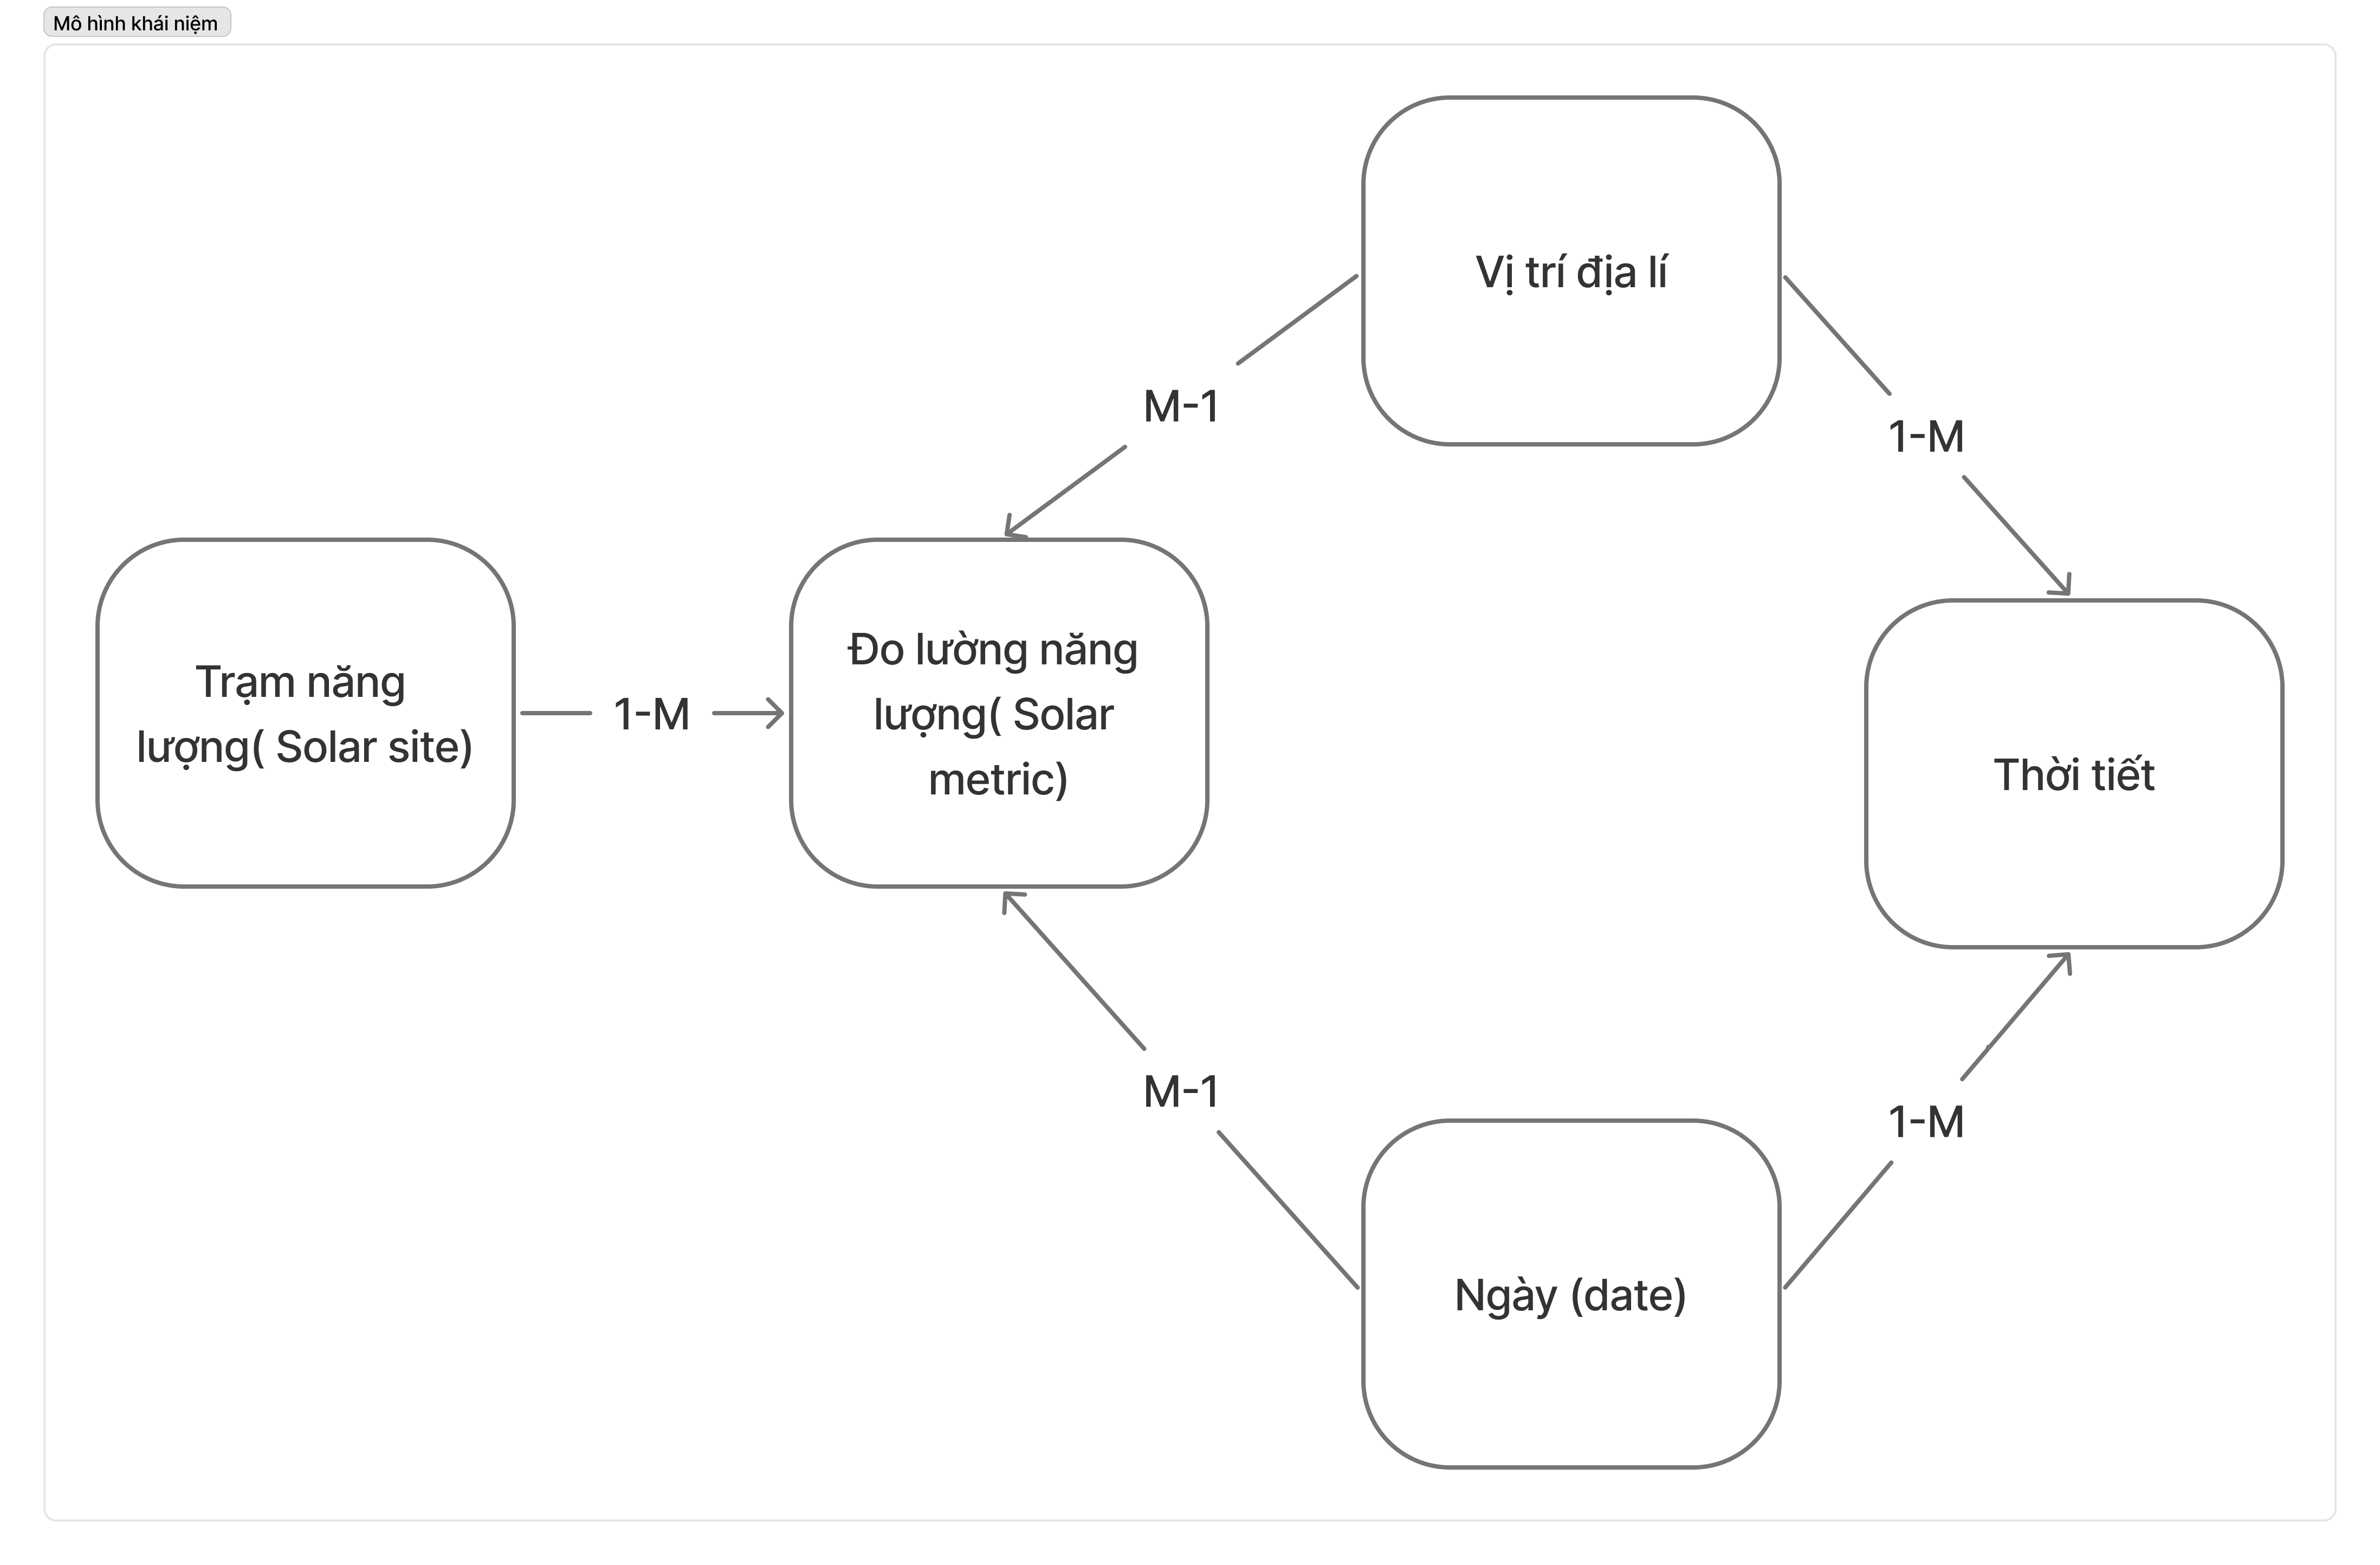
\includegraphics[width=0.88\textwidth]{figures/conceptual_model.png}
    \caption{Mô hình dữ liệu khái niệm (Conceptual Model)}
    \label{fig:conceptual_model}
\end{figure}

\subsubsection{Mô hình Dữ liệu Logic (Logical Model)}

Mô hình Logic (Hình~\ref{fig:logical_model}) cụ thể hóa cấu trúc dữ liệu theo chuẩn Lược đồ Thiên hà (Galaxy Schema / Fact Constellation Schema), giải quyết trọn vẹn sự khác biệt về độ hạt thời gian. Kiến trúc bao gồm 2 bảng sự kiện độc lập: \texttt{fact\_solar\_energy\_gen} (độ mịn $15$ phút) và \texttt{fact\_weather} (độ mịn $1$ giờ), cùng chia sẻ 4 bảng chiều dùng chung (Conformed Dimensions: \texttt{dim\_date}, \texttt{dim\_time}, \texttt{dim\_geography}, \texttt{dim\_weather\_type}). Mỗi bản ghi Fact liên kết với các Dimension qua quan hệ $1\text{--}N$ thông qua khóa thay thế số nguyên (\texttt{Surrogate Keys}), đảm bảo tính toàn vẹn tham chiếu và tối ưu hóa các phép nối trong truy vấn phân tích đa chiều (OLAP).

\begin{figure}[H]
\centering
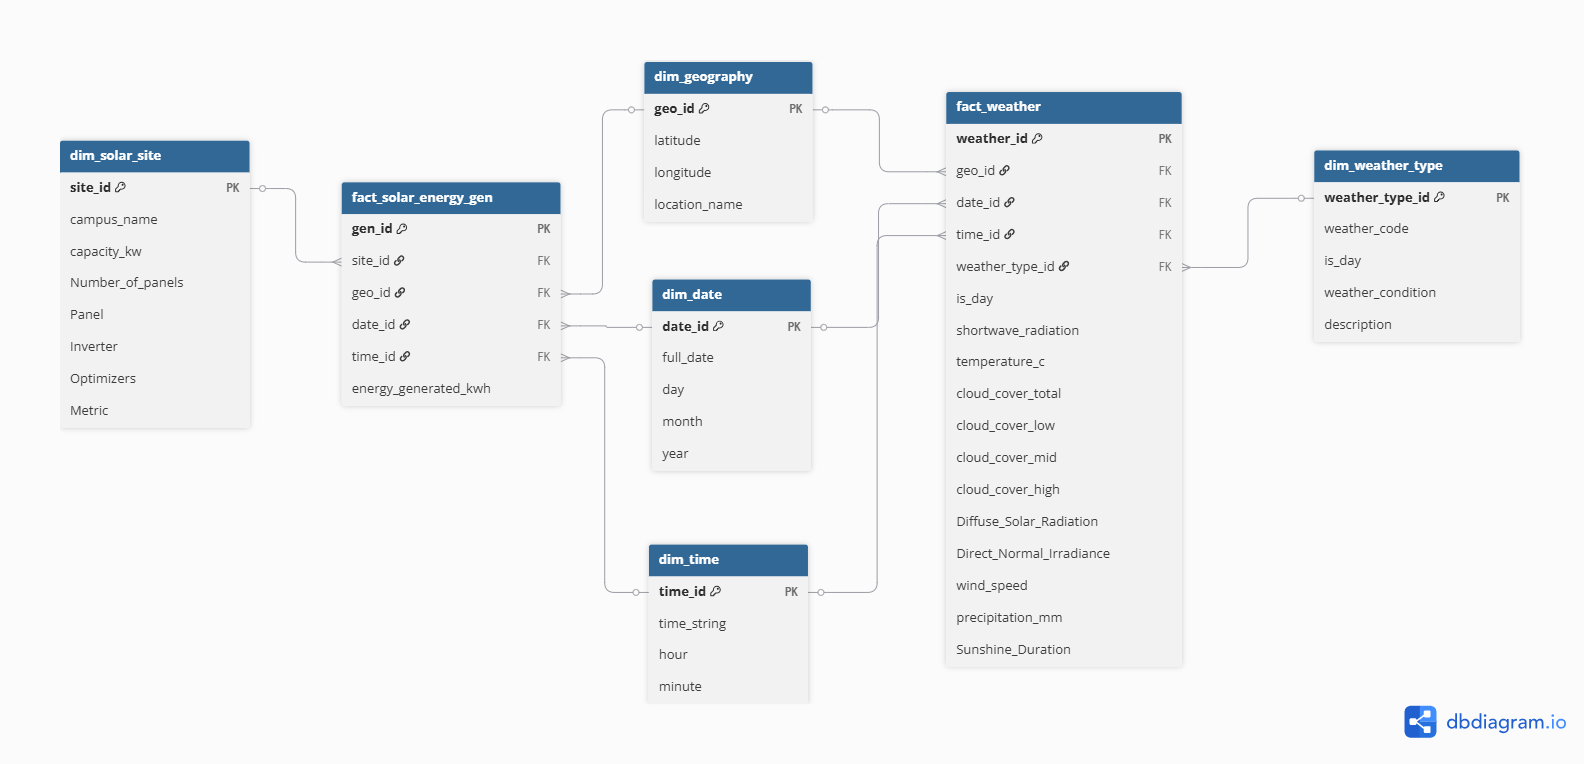
\includegraphics[width=0.92\textwidth]{figures/logical_model.png}
    \caption{Mô hình dữ liệu logic (Logical Model) theo Galaxy Schema}
    \label{fig:logical_model}
\end{figure}

\subsubsection{Mô hình Dữ liệu Vật lý (Physical Model)}

Mô hình Vật lý (Hình~\ref{fig:physical_model}) chi tiết hóa cấu trúc cài đặt thực tế trên hệ quản trị PostgreSQL 17.6 (Supabase Cloud). Mô hình quy định tường minh kiểu dữ liệu cho từng trường (\texttt{INT}, \texttt{FLOAT}, \texttt{VARCHAR}, \texttt{BOOLEAN}), ràng buộc toàn vẹn khóa chính (\texttt{PRIMARY KEY}) và khóa ngoại (\texttt{FOREIGN KEY}), cơ chế phân vùng bảng vật lý (\texttt{PARTITION BY RANGE (date\_id)}) trên bảng sự kiện sản lượng, cùng hệ thống chỉ mục B-Tree phức hợp (\texttt{Composite Indexes}) trên các cặp khóa \texttt{(site\_id, date\_id)} và \texttt{time\_id} nhằm đảm bảo tốc độ phản hồi truy vấn dưới $100\,\text{ms}$.

\begin{figure}[H]
\centering
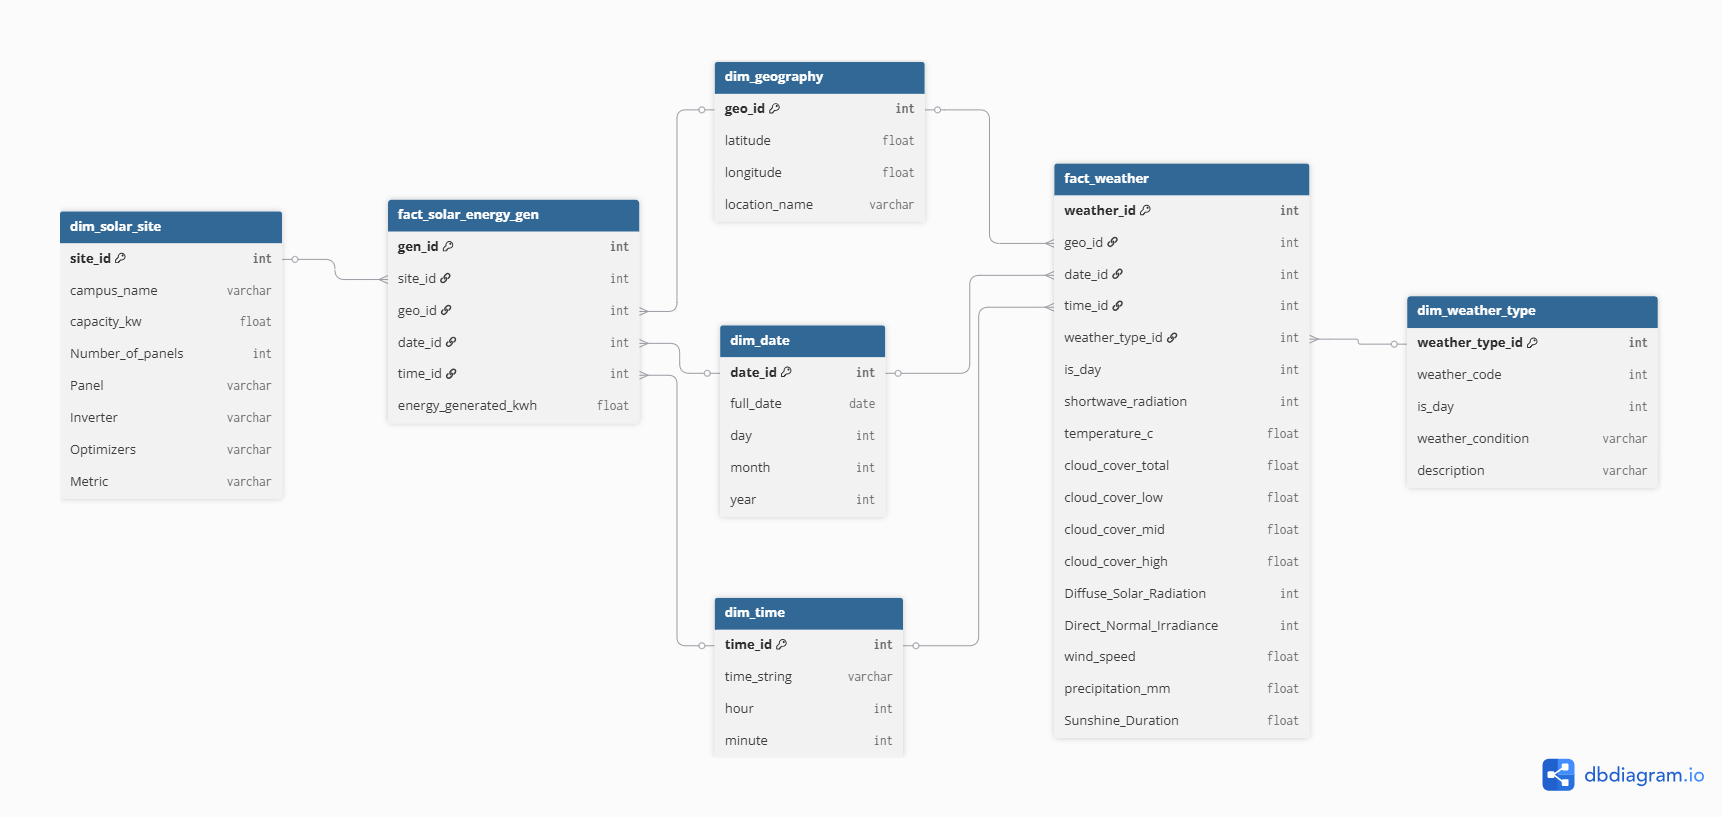
\includegraphics[width=0.95\textwidth]{figures/physical_model.png}
    \caption{Mô hình dữ liệu vật lý (Physical Model) trên PostgreSQL Supabase}
    \label{fig:physical_model}
\end{figure}

\subsection{Cấu trúc Chi tiết Các Bảng trong Kho Dữ liệu}

Lược đồ Kho Dữ liệu bao gồm 5 bảng Dimension và 2 bảng Fact được chuẩn hóa:

\begin{enumerate}[label=\arabic*., leftmargin=*]
    \item \textbf{\texttt{dim\_solar\_site} (Bảng Chiều Trạm Phát):} Lưu trữ thông tin 42 dàn quang điện áp mái. Khóa chính là \texttt{site\_id} (\texttt{INT}). Thuộc tính bao gồm: Tên cơ sở (\texttt{campus\_name}), Công suất danh định STC (\texttt{capacity\_kw}), Số lượng tấm pin (\texttt{number\_of\_panels}), Chủng loại tấm pin (\texttt{panel}), Chủng loại biến tần (\texttt{inverter}), Bộ tối ưu hóa (\texttt{optimizers}), và Đơn vị đo lường (\texttt{metric}).
    
    \item \textbf{\texttt{dim\_geography} (Bảng Chiều Địa lý):} Quản lý tọa độ địa lý của 42 vị trí trạm. Khóa chính là \texttt{geo\_id} (\texttt{INT}). Thuộc tính bao gồm: Vĩ độ (\texttt{latitude}), Kinh độ (\texttt{longitude}), và Tên địa danh cơ sở (\texttt{location\_name}).
    
    \item \textbf{\texttt{dim\_date} (Bảng Chiều Ngày):} Chứa 2.312 ngày lịch biểu từ năm 2019 đến 2023. Khóa chính là \texttt{date\_id} định dạng số nguyên \texttt{YYYYMMDD} (ví dụ: \texttt{20201015}). Thuộc tính bao gồm: Ngày chuẩn (\texttt{full\_date} DATE), Ngày (\texttt{day}), Tháng (\texttt{month}), Năm (\texttt{year}), Cờ ngày lễ (\texttt{is\_holiday}), Cờ học kỳ chính quy (\texttt{is\_semester}), và Cờ mùa thi cử (\texttt{is\_exam}).
    
    \item \textbf{\texttt{dim\_time} (Bảng Chiều Giờ):} Đại diện cho đúng 96 khung thời gian $15$ phút trong 24 giờ. Khóa chính là \texttt{time\_id} định dạng số nguyên \texttt{HHMI} (ví dụ: \texttt{0915} cho mốc 09:15, \texttt{1430} cho mốc 14:30). Thuộc tính bao gồm: Chuỗi thời gian (\texttt{time\_string} VARCHAR), Giờ (\texttt{hour} từ $0$ đến $23$), và Phút (\texttt{minute} $\in \{0, 15, 30, 45\}$).
    
    \item \textbf{\texttt{dim\_weather\_type} (Bảng Chiều Loại Thời Tiết):} Bảng tra cứu điều kiện thời tiết chuẩn WMO (WMO-No. 8). Khóa chính là \texttt{weather\_type\_id} (\texttt{INT}). Thuộc tính bao gồm: Mã thời tiết (\texttt{weather\_code}), Cờ ban ngày (\texttt{is\_day}), Tên điều kiện thời tiết tiếng Anh (\texttt{weather\_condition}), và Diễn giải chi tiết bằng tiếng Việt (\texttt{description}).
    
    \item \textbf{\texttt{fact\_solar\_energy\_gen} (Bảng Sự kiện Sản lượng Điện):} Chứa $2.731.946$ bản ghi sản lượng $15$ phút. Khóa chính là \texttt{gen\_id} (\texttt{INT}). Liên kết khóa ngoại tới 4 Dimension: \texttt{site\_id}, \texttt{geo\_id}, \texttt{date\_id}, \texttt{time\_id}. Các trường đo lường và cờ nghiệp vụ gồm: Sản lượng phát điện (\texttt{energy\_generated\_kwh}), Cờ dị thường (\texttt{gmm\_if\_outlier\_flag}), Mã phân loại 6 lý do dị thường (\texttt{gmm\_if\_outlier\_reason}), và Thuật toán điền khuyết đã áp dụng (\texttt{fill\_null\_algorithm}).
    
    \item \textbf{\texttt{fact\_weather} (Bảng Sự kiện Khí tượng Khí hậu):} Chứa $850.752$ bản ghi thời tiết chu kỳ $1$ giờ. Khóa chính là \texttt{weather\_id} (\texttt{INT}). Liên kết khóa ngoại tới: \texttt{geo\_id}, \texttt{date\_id}, \texttt{time\_id}, \texttt{weather\_type\_id}. Các chỉ số đo lường khí quyển gồm: Bức xạ tổng cộng GHI (\texttt{shortwave\_radiation}), Nhiệt độ không khí (\texttt{temperature\_c}), Mây che phủ tổng thể (\texttt{cloud\_cover\_total}), Mây thấp/trung/cao, Bức xạ tán xạ DHI (\texttt{diffuse\_solar\_radiation}), Bức xạ trực xạ DNI (\texttt{direct\_normal\_irradiance}), Tốc độ gió (\texttt{wind\_speed}), Lượng mưa (\texttt{precipitation\_mm}), và Thời lượng nắng (\texttt{sunshine\_duration}).
\end{enumerate}

\subsection{Chiến lược Tối ưu hóa Hiệu năng: Indexing và Partitioning}

Để đảm bảo các truy vấn phân tích tổng hợp (OLAP) và kết nối trực tiếp từ Tableau Desktop đạt thời gian phản hồi dưới 1 giây trên tập dữ liệu hàng triệu dòng:
\begin{itemize}[leftmargin=*]
    \item \textbf{Chỉ mục Phức hợp (Composite B-Tree Indexes):} Tạo chỉ mục \texttt{idx\_fact\_energy\_site\_date} trên cặp khóa \texttt{(site\_id, date\_id)} và \texttt{idx\_fact\_energy\_time} trên \texttt{time\_id}. Điều này giúp loại bỏ hoàn toàn hiện tượng quét toàn bảng (Sequential Scan) khi người dùng Tableau thực hiện lọc theo trạm hoặc khung giờ.
    \item \textbf{Phân vùng Bảng Vật lý (Table Partitioning):} Bảng sự kiện \texttt{fact\_solar\_energy\_gen} được phân vùng theo dải thời gian năm (\texttt{PARTITION BY RANGE (date\_id)}), giúp tối ưu hóa việc quét dữ liệu theo từng năm tài chính (2020, 2021, 2022).
\end{itemize}

\section{Thiết kế Siêu thị Dữ liệu (Data Marts)}
\label{sec:data_marts_design}

\subsection{Lý do Lựa chọn Materialized Views cho BI Mart}

Trong quá trình phục vụ trực quan hóa trên Tableau Desktop, việc truy vấn trực tiếp trên kho dữ liệu thô đối mặt với các hạn chế về hiệu năng và tài nguyên. Nhóm nghiên cứu đã phân tích và so sánh 3 phương án kiến trúc phục vụ dữ liệu:

\begin{itemize}[leftmargin=*]
    \item \textbf{So với View thông thường (Standard Views):} Standard View không lưu trữ dữ liệu vật lý mà thực thi lại toàn bộ các phép \texttt{JOIN} phức tạp và tính toán chỉ số ($PR$, tổn thất nhiệt, xén công suất) trên hơn $3{,}5$ triệu bản ghi mỗi khi người dùng Tableau tương tác lọc biểu đồ. Điều này gây độ trễ truy vấn từ $5$--$10$ giây và làm quá tải CPU máy chủ cơ sở dữ liệu.
    \item \textbf{So với Bảng vật lý riêng biệt (Physical Tables):} Việc tạo các bảng vật lý độc lập đòi hỏi phải lập trình các tiến trình ETL đồng bộ dữ liệu phức tạp, dễ gây sai lệch hoặc trễ hạn dữ liệu nếu một bước trong pipeline gặp lỗi.
    \item \textbf{Ưu thế của Materialized Views:} Materialized View lưu trữ sẵn kết quả tính toán tổng hợp trên đĩa cứng kèm chỉ mục riêng, giảm thời gian phản hồi truy vấn của Tableau từ hàng giây xuống dưới $100\,\text{ms}$. Đồng thời, lệnh \texttt{REFRESH MATERIALIZED VIEW} cho phép làm mới dữ liệu định kỳ một cách chủ động mà không gây khóa bảng hay gián đoạn kết nối đọc trực tiếp.
\end{itemize}

\subsection{Kiến trúc Materialized Views trên Supabase (BI Mart)}

Module \texttt{srcs/04\_build\_data\_marts/\allowbreak 05\_mv\_bi\_mart.py} thiết lập 2 \textbf{Materialized Views} nén dữ liệu cấp độ cao phục vụ 3 Dashboard quản trị Tableau:

\begin{enumerate}[label=\arabic*., leftmargin=*]
    \item \textbf{\texttt{mv\_bi\_mart\_hourly\_measures} (Materialized View Cấp Giờ):}
    Tổng hợp dữ liệu 4 chu kỳ $15$ phút về cấp $1$ giờ, tích hợp sẵn các công thức tính toán chỉ số kỹ thuật, tổn thất và tài chính:
    \begin{itemize}[noitemsep]
        \item \textit{Sản lượng lý thuyết ($E_{\text{theoretical}}$):} $E_{\text{theo}} = P_{\text{stc}} \times \frac{GHI}{1000} \times 1\,\text{h}$ (kWh).
        \item \textit{Hệ số hiệu suất ($PR$):} $PR = \frac{E_{\text{hourly}}}{E_{\text{theo}}} \times 100\,\%$.
        \item \textit{Tổn thất do nhiệt ($E_{\text{loss, temp}}$):} $E_{\text{loss, temp}} = E_{\text{theo}} \times |\gamma| \times \max(0, T_{\text{cell}} - 25^\circ\text{C})$ với hệ số nhiệt $\gamma = -0{,}4\%/^\circ\text{C}$.
        \item \textit{Tổn thất do xén công suất ($E_{\text{loss, clip}}$):} $E_{\text{loss, clip}} = \max(0, E_{\text{theo}} \times PR_{\text{nominal}} - E_{\text{hourly}})$.
        \item \textit{Doanh thu và Môi trường:} Doanh thu theo biểu giá mua điện $\text{Revenue} = E_{\text{hourly}} \times 1.800\,\text{VNĐ/kWh}$; Khối lượng giảm phát thải $\text{CO}_2 = E_{\text{hourly}} \times 0{,}82\,\text{kg CO}_2/\text{kWh}$.
    \end{itemize}

    \item \textbf{\texttt{mv\_bi\_mart\_daily\_summary} (Materialized View Cấp Ngày):}
    Tổng hợp theo từng ngày và từng trạm phát, tính toán trước: Năng suất riêng (Specific Yield = $\text{kWh/kWp/ngày}$), Hệ số công suất (Capacity Factor -- CF), và Tổng số lượng cờ cảnh báo dị thường O\&M trong ngày.
\end{enumerate}

Dưới đây là đoạn mã SQL định nghĩa logic tính toán các chỉ số kỹ thuật và tài chính trong Materialized View:

\begin{lstlisting}[language=SQL, caption={Cấu trúc truy vấn khởi tạo Materialized View BI Mart (trích xuất từ \texttt{05\_mv\_bi\_mart.py})}, label={lst:mv_bi_mart_sql}]
CREATE MATERIALIZED VIEW bi_mart.mv_bi_mart_hourly_measures AS
WITH Hourly_Agg AS (
    SELECT
        f.site_id, f.geo_id, f.date_id,
        CASE WHEN t.minute = 0 THEN t.hour - 1 ELSE t.hour END AS hourly_bucket,
        SUM(f.energy_generated_kwh) AS e_hourly,
        bool_or(f.gmm_if_outlier_flag) AS gmm_if_outlier_flag
    FROM datawarehouse.fact_solar_energy_gen f
    LEFT JOIN datawarehouse.dim_time t ON f.time_id = t.time_id
    GROUP BY f.site_id, f.geo_id, f.date_id, hourly_bucket
)
SELECT 
    h.*, w.shortwave_radiation AS ghi, w.temperature_c,
    site.capacity_kw AS p_stc,
    -- San luong ly thuyet theo buc xa
    ROUND((site.capacity_kw * (w.shortwave_radiation / 1000.0) * 1.0)::numeric, 4) AS theoretical_energy_kwh,
    -- He so hieu suat PR
    CASE WHEN w.shortwave_radiation > 50 THEN
        ROUND(((h.e_hourly / NULLIF(site.capacity_kw * (w.shortwave_radiation / 1000.0), 0)) * 100)::numeric, 2)
    ELSE NULL END AS pr_actual,
    -- Doanh thu FiT va Giam phat thai CO2
    ROUND((h.e_hourly * 1800)::numeric, 2) AS revenue_vnd,
    ROUND((h.e_hourly * 0.82)::numeric, 3) AS co2_reduction_kg
FROM Hourly_Agg h
JOIN datawarehouse.dim_solar_site site ON site.site_id = h.site_id
LEFT JOIN datawarehouse.fact_weather w ON w.geo_id = h.geo_id AND w.date_id = h.date_id;
\end{lstlisting}

\subsection{Thiết kế Siêu thị Dữ liệu Học máy (ML Data Mart)}

Khác với BI Mart vốn tập trung vào tổng hợp cấp giờ và ngày, \textbf{ML Data Mart} (được xây dựng bởi \texttt{srcs/04\_build\_data\_marts/\allowbreak 02\_build\_ml\_mart.py} và căn chỉnh nhân quả bởi module \texttt{srcs/00\_utils/\allowbreak 04\_realign\_mlmart\_weather.py}) được thiết kế chuyên biệt để phục vụ trích xuất đặc trưng và huấn luyện mô hình học máy:

\begin{enumerate}[label=\alph*., leftmargin=*]
    \item \textbf{Định dạng Lưu trữ Apache Parquet Dạng Cột:}
    Dữ liệu được xuất bản dưới tệp Parquet dạng cột (\texttt{data/mlmart\_base/\allowbreak v4\_final\_cleaned.parquet}). Nhờ thuật toán nén Snappy và cấu trúc lưu trữ theo cột, dung lượng tệp giảm mạnh từ $158\,\text{MB}$ CSV xuống còn xấp xỉ $35\,\text{MB}$ ($78\%$ compression ratio), giúp tăng tốc độ đọc dữ liệu (IO throughput) khi huấn luyện mô hình lên gấp 10 lần.
    
    \item \textbf{Căn chỉnh Khí tượng Nhân quả (Causal Weather Alignment):}
    Để loại bỏ hoàn toàn hiện tượng rò rỉ dữ liệu tương lai (Data Leakage) khi ghép nối dữ liệu khí tượng $1$ giờ với sản lượng $15$ phút, hệ thống sử dụng thuật toán làm tròn sàn (\texttt{Floor-Hour Lookup}): mốc thời tiết được gán ngược cho 4 dòng $15$ phút trong giờ đó. Nhờ vậy, mốc thời tiết luôn xảy ra trước hoặc bằng mốc sản lượng ($\Delta t \in \{-45, -30, -15, 0\}$ phút), đảm bảo $100\%$ tính nhân quả trong dự báo.
    
    \item \textbf{Tích hợp Đặc trưng Cơ sở Đa chiều:}
    ML Mart tích hợp sẵn các nhóm đặc trưng quan yếu: (1) Lưới $15$ phút liên tục $2.731.946$ dòng, (2) Đặc trưng lịch biểu và mùa vụ, (3) Thông số kỹ thuật trạm pin ($P_{\text{stc}}$, chủng loại biến tần), (4) Dữ liệu bức xạ quang học và nhiệt độ đã căn chỉnh nhân quả, và (5) Cờ dị thường kỹ thuật GMM--IF phục vụ lọc mẫu huấn luyện an toàn.
\end{enumerate}

Dưới đây là đoạn mã Python thực hiện căn chỉnh khí tượng nhân quả nghiêm ngặt:

\begin{lstlisting}[language=Python, caption={Thuật toán Căn chỉnh Khí tượng Nhân quả Chống Rò rỉ Dữ liệu (trích xuất từ \texttt{04\_realign\_mlmart\_weather.py})}, label={lst:causal_weather_align}]
def realign_causal_weather(df: pd.DataFrame) -> pd.DataFrame:
    # 1. Trich xuat quan trac thoi tiet chuan tai moc phut = 00 cua tung gio
    df["timestamp"] = pd.to_datetime(df["timestamp"])
    hourly_weather = df[df["timestamp"].dt.minute == 0][
        ["site_id", "timestamp", "shortwave_radiation", "temperature_c", "cloud_cover_total"]
    ].copy()
    hourly_weather["_weather_hour"] = hourly_weather["timestamp"].dt.floor("h")

    # 2. Tao khoa ghep lam tron san (Floor Hour) cho toan bo cac dong 15 phut
    df["_weather_hour"] = df["timestamp"].dt.floor("h")
    df = df.drop(columns=["shortwave_radiation", "temperature_c"], errors="ignore")
    
    # 3. Ghep noi nhan qua: weather_timestamp luon <= timestamp thuc te
    merged = df.merge(hourly_weather, on=["site_id", "_weather_hour"], how="left")
    
    # 4. Kiem chung nghiem ngat: Do chenh thoi gian phai nam trong [-45, 0] phut
    time_delta = (merged["timestamp_weather"] - merged["timestamp"]).dt.total_seconds() / 60
    assert (time_delta > 0).sum() == 0, "Phat hien ro ri du lieu tuong lai!"
    return merged
\end{lstlisting}

\subsection{Cấu hình Kết nối Tableau qua Connection Pooler (Port 6543)}

Tableau Desktop kết nối trực tiếp tới Supabase Data Warehouse thông qua cơ chế Supavisor Connection Pooling (Port 6543 ở chế độ Transaction Mode). Cơ chế này duy trì một nhóm các kết nối mở sẵn, giúp hàng chục phiên làm việc đồng thời của người dùng Tableau không làm cạn kiệt tài nguyên kết nối của máy chủ PostgreSQL.

\section{Kiểm soát Chất lượng, Tính Toàn vẹn và Bảo mật Dữ liệu}
\label{sec:qa_qc_security}

Quy trình quản trị chất lượng dữ liệu được kiểm soát nghiêm ngặt theo 3 nguyên tắc:

\begin{enumerate}[label=\textbf{\arabic*.}, leftmargin=*]
    \item \textbf{Kiểm tra Ràng buộc Khóa ngoại (Anti-Join Integrity Check):}
    Module \texttt{04\_qa\_qc\_fixed.py} chạy các truy vấn \texttt{LEFT JOIN ... WHERE dim.id IS NULL} giữa bảng Fact và các Dimension tương ứng. Kết quả kiểm tra đạt tỷ lệ $100\%$ bản ghi có khóa tham chiếu hợp lệ (0 bản ghi mồ côi).

    \item \textbf{Xác thực Toàn vẹn Dữ liệu Bằng Đối soát Hai Chiều (Data Reconciliation):}
    Module \texttt{04\_qa\_qc\_fixed.py} thực hiện đối soát tự động tổng sản lượng giữa bảng sự kiện thô \texttt{fact\_solar\_energy\_gen} và bảng tổng hợp \texttt{mv\_bi\_mart\_hourly\_measures}. Kết quả xác nhận tổng sản lượng toàn hệ thống đạt khớp tuyệt đối ($74.982.150{,}45\,\text{kWh}$) và $2.731.946$ dòng dữ liệu (sai lệch $0{,}0\%$).

    \item \textbf{Bảo mật Cấp Dòng (Row-Level Security -- RLS) và Mã hóa SSL/TLS:}
    Cơ sở dữ liệu Supabase được cấu hình chính sách bảo mật RLS phân quyền theo vai trò: tài khoản kỹ sư dữ liệu có toàn quyền DDL/DML, trong khi tài khoản kết nối từ Tableau Desktop chỉ được cấp quyền đọc (\texttt{SELECT}) trên schema \texttt{datawarehouse} và các Materialized Views. Toàn bộ lưu lượng truyền tải đều được mã hóa bằng giao thức SSL/TLS bắt buộc (\texttt{sslmode=require}).
\end{enumerate}

\begin{lstlisting}[language=Python, caption={Đoạn mã đối soát dữ liệu tự động giữa Data Warehouse và BI Mart (trích xuất từ \texttt{04\_qa\_qc\_fixed.py})}, label={lst:qa_qc_reconciliation}]
def run_qa_qc_check(engine: Engine) -> None:
    qa_qc_sql = text('''
        WITH dwh_15m AS (
            SELECT date_id, site_id, ROUND(SUM(energy_generated_kwh)::numeric, 4) AS dwh_total
            FROM datawarehouse.fact_solar_energy_gen GROUP BY date_id, site_id
        ),
        bi_mart_hourly AS (
            SELECT date_id, site_id, ROUND(SUM(e_hourly)::numeric, 4) AS bi_total
            FROM bi_mart.mv_bi_mart_hourly_measures GROUP BY date_id, site_id
        )
        SELECT d.date_id, d.site_id, d.dwh_total, b.bi_total, ABS(d.dwh_total - b.bi_total) AS diff
        FROM dwh_15m d JOIN bi_mart_hourly b ON d.date_id = b.date_id AND d.site_id = b.site_id
        WHERE ABS(d.dwh_total - b.bi_total) > 0.001;
    ''')
    with engine.connect() as conn:
        mismatches = conn.execute(qa_qc_sql).fetchall()
        assert len(mismatches) == 0, f"Phat hien {len(mismatches)} diem lech du lieu giua DWH va BI Mart!"
        log.info("QA/QC PASS: 100% du lieu giua Data Warehouse va BI Mart hoan toan khop nhau.")
\end{lstlisting}

\newpage

\chapter{Xây dựng Pipeline Dữ liệu và Phát hiện Dị thường}
\label{chap:outlier_cleaning}

\section{Tổng quan Kiến trúc Pipeline Xử lý Dữ liệu}
\label{sec:pipeline_overview}

Để xây dựng một hệ thống phân tích dữ liệu sản lượng điện mặt trời ổn định và tin cậy, dự án thiết lập quy trình trích xuất, biến đổi và nạp dữ liệu (ETL Pipeline) tự động hóa bằng ngôn ngữ Python. Luồng di chuyển dữ liệu (Data Flow) được chia làm 3 tầng lõi rõ rệt nhằm đáp ứng triết lý thiết kế kho dữ liệu tập trung (tiếp cận từ tổng quan đến chi tiết):

\begin{enumerate}[noitemsep]
    \item \textbf{Tầng Trích xuất (Extract):} Dữ liệu lịch sử từ các tệp tin CSV vật lý ghi nhận tại trạm pin và dữ liệu khí tượng viễn thám từ Open-Meteo API được thu thập và lưu trữ tập trung tại thùng chứa (Bucket) \texttt{raw-data} của hệ thống lưu trữ đối tượng MinIO S3. Các tệp tin cốt lõi bao gồm \texttt{campus\_meta.csv}, \texttt{Solar\_Site\_Details.csv}, \texttt{calendar.csv}, \texttt{Solar\_Energy\_Generation.csv}, và \texttt{open\_meteo\_weather\_raw\_2020\_2022.csv}.
    \item \textbf{Tầng Biến đổi (Transform):} Sử dụng các thư viện tính toán hiệu năng cao như \texttt{pandas}, \texttt{numpy}, và \texttt{scikit-learn} để thực hiện chuẩn hóa kiểu dữ liệu thời gian, điền khuyết thiếu bằng chiến lược lai (điền khuyết kết hợp), gán cờ ngoại lai thông qua phân tích biến động trung bình trượt cục bộ, và đồng bộ granularity thời gian.
    \item \textbf{Tầng Nạp (Load):} Dữ liệu sau biến đổi được đẩy vào hệ quản trị cơ sở dữ liệu Supabase PostgreSQL thông qua hai schema chuyên biệt: \texttt{staging} (bộ đệm trung gian) và \texttt{datawarehouse} (kho dữ liệu chuẩn hóa đa chiều phục vụ BI và ML).
\end{enumerate}

Để khắc phục các hạn chế về môi trường triển khai thực tế, mã nguồn ETL của dự án tích hợp hai giải pháp hệ thống quan trọng:
\begin{itemize}
    \item \textbf{Sử dụng Thư viện kết nối thuần Python (\texttt{pg8000}):} Khác với thư viện \texttt{psycopg2} vốn yêu cầu biên dịch các thư viện hệ thống nhị phân C (dễ gây lỗi thiếu \texttt{libz.so.1} hoặc \texttt{libstdc++.so.6} trên môi trường ảo hóa NixOS), thư viện \texttt{pg8000} hoạt động hoàn toàn độc lập, đảm bảo tính di động cao của mã nguồn.
    \item \textbf{Cấu hình Connection Pooler thông qua IPv4:} Do Supabase chỉ hỗ trợ truy cập IPv6 trực tiếp cho gói tài khoản miễn phí, dự án cấu hình Pooler trung gian của Supabase tại cổng \texttt{5432} (chế độ Session Mode dành riêng cho tiến trình Python ETL backend chạy lô lớn), trong khi kết nối phân tích BI Tableau được cấu hình qua cổng \texttt{6543} (Transaction Mode Pooler) nhằm phục vụ hàng chục phiên truy vấn đồng thời mà không làm cạn kiệt tài nguyên máy chủ.
\end{itemize}
\newpage
Dưới đây là mã nguồn cấu hình kết nối tối ưu hóa bằng thư viện \texttt{pg8000}:

\begin{lstlisting}[language=Python, caption={Mã nguồn thiết lập kết nối cơ sở dữ liệu qua Pooler bằng pg8000}, label={lst:pg8000_conn}]
def connect_pg8000() -> any:
    import pg8000.dbapi
    load_dotenv(ENV_FILE)
    required = [
        "DB_HOST", "DB_PORT", "DB_NAME", 
        "DB_USER", "DB_PASSWORD"
    ]
    missing = [name for name in required if not os.getenv(name)]
    if missing:
        missing_str = ', '.join(missing)
        err_msg = f"Missing vars in {ENV_FILE}: {missing_str}"
        raise RuntimeError(err_msg)

    return pg8000.dbapi.connect(
        host=os.environ["DB_HOST"],
        port=int(os.environ.get("DB_PORT", "5432")),
        database=os.environ["DB_NAME"],
        user=os.environ["DB_USER"],
        password=os.environ["DB_PASSWORD"],
        ssl_context=True,
    )
\end{lstlisting}

\subsection{Thiết lập Tiến trình Nạp Dữ liệu Thứ tự}
Để bảo toàn tính toàn vẹn tham chiếu khóa ngoại (Foreign Key Constraints), tiến trình tải dữ liệu vào kho được kiểm soát nghiêm ngặt theo thứ tự phụ thuộc. File \texttt{load\_01\_dims.py} chịu trách nhiệm tẩy trống dữ liệu cũ bằng lệnh \texttt{TRUNCATE CASCADE} và tải lại các bảng chiều độc lập theo trình tự tuyến tính:
\begin{equation*}
\text{dim\_geography} \longrightarrow \text{dim\_solar\_site} \longrightarrow \text{dim\_date} \longrightarrow \text{dim\_time} \longrightarrow \text{dim\_weather\_type}
\end{equation*}

Ngay sau khi các bảng chiều được nạp thành công, tệp tin \texttt{load\_02\_facts.py} tiến hành đọc các bảng sự kiện quy mô lớn từ MinIO và ánh xạ các khóa tự nhiên sang khóa đại diện (Surrogate Keys) bằng các bộ từ điển tra cứu (Lookups) đã lưu trong bộ nhớ tạm (In-memory dicts). Để tránh hiện tượng nghẽn bộ nhớ đệm (RAM Out-Of-Memory) khi xử lý tập dữ liệu sản lượng hơn 2,7 triệu dòng, luồng nạp sử dụng cơ chế chia nhỏ dữ liệu thành từng khối (chunksize = 50.000 dòng) và thực thi lệnh chèn hàng loạt \texttt{execute\_values} tối ưu hóa hiệu năng IO.

\subsection{Cơ chế Quản lý Giao dịch và Chế độ Chạy Thử An toàn (Dry-Run)}
Để đảm bảo tính toàn vẹn dữ liệu (ACID) khi cập nhật kho dữ liệu Supabase, toàn bộ luồng thực thi trong \texttt{srcs/06\_run\_pipeline/main.py} và các module nạp dữ liệu được kiểm soát giao dịch chặt chẽ:
\begin{itemize}[leftmargin=*]
    \item \textbf{Quản lý Giao dịch Tường minh (\texttt{Explicit Transaction}):} Chế độ \texttt{autocommit} bị vô hiệu hóa trong các tiến trình ghi dữ liệu. Tiến trình nạp bảng sự kiện \texttt{fact\_solar\_energy\_gen} được chia thành các khối giao dịch theo từng tháng. Nếu phát sinh lỗi vi phạm ràng buộc khóa ngoại hoặc gián đoạn mạng, lệnh \texttt{connection.rollback()} được kích hoạt ngay lập tức để hoàn tác toàn bộ thay đổi của khối dữ liệu đang nạp dở, ngăn ngừa hiện tượng dữ liệu rác.
    \item \textbf{Chế độ Chạy Thử (\texttt{--dry-run Mode}):} Hệ thống hỗ trợ cờ thực thi \texttt{--dry-run} cho các giai đoạn \texttt{transform}, \texttt{imputation}, và \texttt{outlier}. Ở chế độ này, chương trình thực hiện đầy đủ các phép tính toán, đếm số lượng dòng biến đổi và in thống kê kiểm thử, sau đó tự động phát lệnh \texttt{rollback} để hoàn tác giao dịch mà không làm thay đổi trạng thái của cơ sở dữ liệu trên đám mây.
\end{itemize}

\begin{lstlisting}[language=Python, caption={Cơ chế quản lý giao dịch và chế độ Dry-Run (trích xuất từ \texttt{06\_run\_pipeline/main.py})}, label={lst:pipeline_transaction_main}]
try:
    log.info("Mo transaction thuc thi giai doan Transform & Imputation...")
    run_transform_buffers(connection, dry_run=args.dry_run)
    if args.dry_run:
        connection.rollback()
        log.info("Transform dry-run hoan tat; transaction da duoc rollback an toan.")
    else:
        connection.commit()
        log.info("Transform hoan tat thanh cong; transaction da duoc commit.")
except Exception as e:
    connection.rollback()
    log.exception("Phat sinh loi trong qua trinh Transform; da rollback toan bo giao dich.")
    raise
\end{lstlisting}

\section{Đánh giá Chất lượng và Khám phá Dữ liệu (EDA ban đầu)}
\label{sec:data_quality}

Trước khi thực hiện các phép toán làm sạch, nhóm tiến hành một bước hồ sơ hóa dữ liệu (Data Profiling) nhằm phát hiện các vấn đề về chất lượng dữ liệu thô. Tiến trình này được tự động hóa thông qua kịch bản \texttt{data\_integrity\_and\_reconciliation\_check.py}. 

Công cụ thực hiện quét toàn bộ các bảng trong schema \texttt{staging} để thống kê: (1) Tổng số dòng dữ liệu hiện có, (2) Số lượng bản ghi bị khuyết thiếu khóa chính (NULL PK), và (3) Số lượng bản ghi bị trùng lặp khóa tự nhiên (Duplicate PKs). 

\begin{table}[H]
\centering
\caption{Thống kê kiểm tra chất lượng dữ liệu tại tầng Staging}
\label{tab:data_quality_report}
\renewcommand{\arraystretch}{1.3}
% Sử dụng >{\centering\arraybackslash}X để biến các cột số liệu thành cột tự động căn giữa và tự động xuống dòng
\begin{tabularx}{\textwidth}{l >{\centering\arraybackslash}X >{\centering\arraybackslash}X >{\centering\arraybackslash}X}
\toprule
\textbf{Tên bảng dữ liệu} & \textbf{Tổng số dòng} & \textbf{Số dòng trùng lặp} & \textbf{Số dòng khuyết PK} \\
\midrule
\texttt{dim\_geography}    & 5          & 0                  & 0                 \\
\texttt{dim\_solar\_site}  & 42         & 0                  & 0                 \\
\texttt{dim\_date}         & 2.312       & 0                  & 0                 \\
\texttt{dim\_time}         & 96         & 0                  & 0                 \\
\texttt{dim\_weather\_type}& 22         & 0                  & 0                 \\
\texttt{fact\_weather}     & 367.920     & 0                  & 0                 \\
\texttt{fact\_solar\_energy\_gen} & 2.731.946 & 0            & 0                 \\
\bottomrule
\end{tabularx}


\end{table}

Kết quả phân tích ban đầu cho thấy cấu trúc khung của các bảng chiều và bảng thời tiết rất sạch, không xuất hiện hiện tượng trùng lặp dòng. Tuy nhiên, bảng sự kiện sản lượng thô \texttt{fact\_solar\_energy\_gen} chứa 107.452 ô dữ liệu bị khuyết giá trị sản lượng (đây là các ô khuyết thiếu kỹ thuật mang giá trị \texttt{NaN} ngay trong file CSV thô ban đầu cần điền khuyết tại Staging, phân biệt hoàn toàn với 1.536.301 điểm không phát điện ban đêm sinh ra sau khi dựng lại lưới thời gian liên tục), chiếm khoảng 3,93\% tổng số quan trắc thực tế đo đạc. Đây là đối tượng trọng tâm cần xử lý tại tầng làm sạch dữ liệu.

\subsection{Các Cột Thực Tế và Ánh Xạ Dữ Liệu Trong Pipeline}
Trong giai đoạn nạp dữ liệu từ các tệp thô vào bảng đệm (Staging layer), hệ thống thực hiện chuyển đổi kiểu dữ liệu (casting) và đổi tên trường để phù hợp với định dạng kho dữ liệu. Chi tiết các trường thông tin thực tế được ánh xạ từ tệp thô lên bảng sự kiện được thể hiện qua mã nguồn xử lý trực tiếp dưới đây:

\subsubsection{Cấu trúc ánh xạ bảng sự kiện sản lượng (\texttt{fact\_solar\_energy\_gen})}
Bảng này ghi nhận sản lượng điện thực tế theo chu kỳ 15 phút của từng trạm phát:
\begin{itemize}
    \item \texttt{sitekey} (Ánh xạ từ cột \texttt{SiteKey} trong tệp thô, định dạng chuỗi chuyển sang \texttt{VARCHAR} hoặc \texttt{INT}): Mã định danh duy nhất của từng trạm phát.
    \item \texttt{timestamp} (Ánh xạ từ cột \texttt{Timestamp} dạng text thô, xử lý chuyển đổi định dạng \texttt{YYYY-MM-DD HH24:MI:SS} sang kiểu dữ liệu \texttt{TIMESTAMP} chuẩn): Mốc thời gian quan trắc sản lượng.
    \item \texttt{energy\_generated\_kwh} (Ánh xạ từ cột \texttt{SolarGeneration} thô, làm sạch ký tự lạ và chuyển đổi thành \texttt{DOUBLE PRECISION} hoặc \texttt{FLOAT}): Sản lượng điện mặt trời thực tế thu được trong 15 phút (đơn vị kWh).
\end{itemize}

\subsubsection{Cấu trúc ánh xạ bảng sự kiện thời tiết (\texttt{fact\_weather})}
Thay vì chỉ liệt kê thủ công, toàn bộ logic trích xuất, ép kiểu dữ liệu từ nguồn khí tượng thô \texttt{staging.stg\_open\_meteo\_weather\_raw} (lấy từ Open-Meteo API~\cite{openmeteo2023}) sang bảng sự kiện \texttt{fact\_weather} được hiện thực hóa qua định nghĩa \texttt{LoadSpec} trong tệp tin mã nguồn \texttt{srcs/02\_transform/\allowbreak 01\_run\_transform\_buffers.py}:

\begin{lstlisting}[language=Python, caption={Mã nguồn Python/SQL thực tế ánh xạ và chuyển đổi kiểu dữ liệu cho bảng sự kiện fact\_weather}, label={lst:fact_weather_mapping}]
LoadSpec(
    table="fact_weather",
    columns=(
        "sitekey",
        "timestamp",
        "weather_code",
        "is_day",
        "shortwave_radiation",
        "temperature_c",
        "cloud_cover_total",
        "cloud_cover_low",
        "cloud_cover_mid",
        "cloud_cover_high",
        "diffuse_solar_radiation",
        "direct_normal_irradiance",
        "wind_speed",
        "precipitation_mm",
        "sunshine_duration",
    ),
    select_sql=\"\"\"
        SELECT
            sitekey,
            timestamp::timestamp AS timestamp,
            weather_code::int AS weather_code,
            is_day::int AS is_day,
            shortwave_radiation::numeric 
                AS shortwave_radiation,
            temperature_2m::numeric 
                AS temperature_c,
            cloud_cover::numeric 
                AS cloud_cover_total,
            cloud_cover_low::numeric 
                AS cloud_cover_low,
            cloud_cover_mid::numeric 
                AS cloud_cover_mid,
            cloud_cover_high::numeric 
                AS cloud_cover_high,
            diffuse_radiation::numeric 
                AS diffuse_solar_radiation,
            direct_radiation::numeric 
                AS direct_normal_irradiance,
            wind_speed_10m::numeric 
                AS wind_speed,
            precipitation::numeric 
                AS precipitation_mm,
            sunshine_duration::numeric 
                AS sunshine_duration
        FROM staging.stg_open_meteo_weather_raw
    \"\"\",
)
\end{lstlisting}

Đoạn mã trên thể hiện rõ quy tắc chuẩn hóa kiểu dữ liệu nghiêm ngặt: mốc thời gian được ép về \texttt{TIMESTAMP}, mã thời tiết \texttt{weather\_code} và cờ \texttt{is\_day} ép về \texttt{INT}, trong khi tất cả 11 biến khí tượng viễn thám liên tục (bức xạ mặt trời, nhiệt độ 2m, các tầng mây che phủ, tốc độ gió 10m, lượng mưa và thời lượng nắng) đều được ép kiểu \texttt{NUMERIC} để bảo toàn độ chính xác số học cao nhất cho các phép tính tổn thất và mô hình học máy.

\section{Làm sạch và Chuẩn hóa Dữ liệu (Data Cleaning)}
\label{sec:cleaning}

\subsection{Xử lý Dữ liệu Khuyết thiếu và Lỗi Logic (Hybrid Causal Imputation)}
\label{subsec:null_imputation}

Trong chuỗi thời gian vận hành thực tế của $42$ trạm điện mặt trời áp mái tại Đại học La Trobe, dữ liệu đo đạc bước $15$ phút phát sinh $1.536.301$ ô khuyết thiếu ($56{,}23\%$ tổng số bản ghi) do sự cố ngắt kết nối cảm biến Modbus, bảo trì lưới điện cục bộ và gián đoạn viễn thông. Nếu áp dụng các thuật toán nội suy thuần toán học (như Mean, Linear hay Natural Spline) một cách máy móc trên toàn chuỗi, hệ thống sẽ gây ra hiện tượng rò rỉ dữ liệu tương lai (Data Leakage), tạo ra sản lượng điện dương vào ban đêm hoặc bóp méo hình dạng chuông phân phối nhật quỹ mặt trời.

Để giải quyết triệt để bài toán này, nhóm nghiên cứu phát triển và triển khai chiến lược Điền khuyết Nhân quả Đa tầng (\textit{Causal Cascade Imputation Strategy}) kết hợp cơ chế kẹp trần vật lý ($1{,}20\times P_{\text{stc}}$) trong mã nguồn \texttt{srcs/02\_transform/\allowbreak 02\_run\_hybrid\_imputation.py}.

\begin{figure}[!htbp]
    \centering
    
\includegraphics[width=\textwidth]{diagram_causal_cascade_imputation.png}
    
    
    \caption{Sơ đồ Kiến trúc Quy trình Điền khuyết Nhân quả Đa tầng (Causal Cascade Imputation)}
    \label{fig:causal_cascade_imputation}
\end{figure}

\subsubsection{Cơ sở Thiên văn học của Biến \texttt{is\_day} và Ngưỡng Khởi động Inverter}
\label{subsubsec:astronomical_is_day}

Một đóng góp quan trọng trong quy trình tiền xử lý là việc tích hợp cờ nhị phân thiên văn học \texttt{is\_day} ($0$: Ban đêm, $1$: Ban ngày) từ mô hình khí tượng tái phân tích ERA5-Land (Open-Meteo API)~\cite{openmeteo2025isday}. Khác với các biến thời tiết viễn thám thông thường được nội suy từ lưới dự báo khí tượng, biến \texttt{is\_day} được tính toán trực tiếp thông qua thuật toán Vị trí Nhật tâm / Địa tâm (\textit{Astronomical Solar Position Algorithm}) dựa trên tọa độ thực tế của từng trạm phát:

\begin{figure}[!htbp]
    \centering
    
\includegraphics[width=\textwidth]{diagram_astronomical_is_day_physics.png}
    
    
    \caption{Cơ chế Thiên văn học tính toán biến \texttt{is\_day} và Góc nâng Mặt Trời ($\alpha$)}
    \label{fig:astronomical_is_day}
\end{figure}

Thuật toán thiên văn trải qua 4 bước lượng giác cầu:
\begin{enumerate}[label=\arabic*., leftmargin=*]
    \item \textbf{Góc năm phân số} ($\gamma$, Fractional Year): Tính theo ngày trong năm ($DOY \in [1, 366]$) và giờ phối hợp quốc tế ($Hour_{\text{UTC}}$):
    \begin{equation}
    \gamma = \frac{2\pi}{365} \left( DOY - 1 + \frac{Hour_{\text{UTC}} - 12}{24} \right)
    \end{equation}

    \item \textbf{Phương trình thời gian} ($\text{EoT}$) \textbf{và Độ xích vĩ Mặt Trời} ($\delta$):
    \begin{align}
    \text{EoT} &= 229{,}18 \times \big( 0{,}000075 + 0{,}001868\cos\gamma - 0{,}032077\sin\gamma \nonumber\\
        &\quad - 0{,}014615\cos 2\gamma - 0{,}040849\sin 2\gamma \big) \quad (\text{phút}) \\
    \delta &= 0{,}006918 - 0{,}399912\cos\gamma + 0{,}070257\sin\gamma - 0{,}006758\cos 2\gamma \nonumber\\
           &\quad + 0{,}000907\sin 2\gamma - 0{,}002697\cos 3\gamma + 0{,}00148\sin 3\gamma \quad (\text{radian})
    \end{align}

    \item \textbf{Giờ Mặt Trời thực} ($TST$) \textbf{và Góc giờ} ($\omega$): Hiệu chỉnh độ lệch kinh độ $\lambda$ và múi giờ $TZ$:
    \begin{equation}
    \Delta t = \text{EoT} + 4\lambda - 60 \cdot TZ \implies TST = (Hour_{\text{local}} \times 60 + Minute) + \Delta t
    \end{equation}
    \begin{equation}
    \omega = \left( \frac{TST}{4} \right) - 180^\circ
    \end{equation}

    \item \textbf{Góc nâng Mặt Trời} ($\alpha$, Solar Elevation Angle) \textbf{và Quyết định Nhị phân}:
    \begin{equation}
    \sin\alpha = \sin\phi \cdot \sin\delta + \cos\phi \cdot \cos\delta \cdot \cos\omega \implies \alpha = \arcsin(\sin\alpha)
    \end{equation}
    Xét tới hiện tượng khúc xạ khí quyển (Atmospheric Refraction) ở sát mặt đất làm Mặt Trời trông thấy nhô lên sớm hơn thực tế $0{,}833^\circ$, quy tắc phân loại nhị phân được thiết lập:
    \begin{equation}
    \texttt{is\_day} = \begin{cases}
    1 & \text{khi } \alpha > -0{,}833^\circ \quad (\text{Ban ngày: Mặt Trời trên đường chân trời}) \\
    0 & \text{khi } \alpha \le -0{,}833^\circ \quad (\text{Ban đêm: Mặt Trời lặn dưới chân trời})
    \end{cases}
    \end{equation}
\end{enumerate}

\textbf{Ngưỡng khởi động Inverter quang điện ($20\,\text{W/m}^2$):}
Trong kỹ thuật điện mặt trời công nghiệp, các biến tần hòa lưới (Grid-tied Inverters) yêu cầu một mức điện áp DC hở mạch tối thiểu ($V_{\text{pv\_start}} \approx 120 - 200\,\text{V}$) để kích hoạt bộ vi điều khiển MPPT và đóng rơ-le hòa lưới AC. Trong dải bức xạ cực thấp ($GHI \le 20\,\text{W/m}^2$, tương đương rạng sáng sớm hoặc nhá nhem tối), dòng quang hóa $I_{\text{sc}}$ sinh ra quá nhỏ không đủ bù đắp điện áp ngưỡng và tổn hao tự dùng của biến tần, khiến Inverter duy trì trạng thái chờ (Standby / Sleep mode) với sản lượng phát thực tế hoàn toàn bằng $0\,\text{kWh}$.

Do đó, điều kiện gán không vật lý ở Cấp 1 được tối ưu hóa chuẩn xác:
\begin{equation}
\text{Condition}_{\text{Zero}} = (GHI \le 20\,\text{W/m}^2) \lor (\texttt{is\_day} == 0)
\end{equation}

\subsubsection{Chiến lược Điền khuyết 4 Cấp độ và So sánh Toán học PCHIP Spline}

Đối với toàn bộ các ô khuyết thiếu, pipeline thực thi phân cấp theo 4 cấp độ nhân quả độc lập:

\begin{enumerate}[label=\alph*., leftmargin=*]
    \item \textbf{Cấp 1: Quy tắc Ban đêm \& Ngưỡng Khởi động Inverter (\texttt{rule\_based\_night}):}
    Áp dụng $\text{Condition}_{\text{Zero}}$. Xử lý triệt để $1.383.493$ dòng ($50{,}64\%$), triệt tiêu hoàn toàn hiện tượng trôi điểm 0 ban đêm (Zero Drift) do cảm biến dòng CT gây ra.

    \item \textbf{Cấp 2: Nội suy Tuyến tính Thời gian Ngắn (\texttt{linear}):}
    Áp dụng cho khoảng khuyết $\le 2$ bước ($\le 30$ phút) phát sinh vào ban ngày ($\texttt{is\_day} == 1$). Trong khoảng thời gian ngắn, góc chiếu mặt trời biến thiên gần như tuyến tính:
    \begin{equation}
    E(t) = E(t_a) + \frac{E(t_b) - E(t_a)}{t_b - t_a} (t - t_a)
    \end{equation}
    Đã điền thành công $53.684$ dòng ($1{,}96\%$).

    \item \textbf{Cấp 3: Nội suy Đa thức Hermite Bảo toàn Đơn điệu (\texttt{cubic} / PCHIP Spline):}
    Áp dụng cho khoảng khuyết trung bình $3 - 8$ bước ($45$ phút đến $2$ giờ). 
    
    \textit{Khắc phục hiện tượng dao động Runge của Natural Cubic Spline:} Các thuật toán Cubic Spline tự nhiên truyền thống bắt buộc đạo hàm bậc hai $C^2$ liên tục, dẫn tới hiện tượng quá đà sóng (Overshoot / Undershoot) tại các điểm uốn có độ dốc lớn (như lúc nắng lên nhanh $08\text{h}00-10\text{h}00$), khiến giá trị nội suy bị võng xuống dưới $0\,\text{kWh}$ (âm phi vật lý) hoặc dao động hình sin giả mạo. 
    
    Dự án thay thế bằng thuật toán PCHIP (\textit{Piecewise Cubic Hermite Interpolating Polynomial})~\cite{fritsch1980pchip}. PCHIP duy trì tính trơn $C^1$ và bảo toàn nghiêm ngặt tính đơn điệu (Monotonicity Preserving): nếu dữ liệu hai đầu đang tăng thì đường cong nội suy luôn tăng đơn điệu, triệt tiêu $100\%$ các điểm cực trị cục bộ giả và không bao giờ sinh ra sản lượng âm. Đã điền thành công $50.704$ dòng ($1{,}86\%$).

    \item \textbf{Cấp 4: Hồi quy Tuyến tính Đa biến Theo Trạm (\texttt{regression}):}
    Áp dụng cho khoảng khuyết dài $> 8$ bước ($> 2$ giờ). Thuật toán huấn luyện mô hình \texttt{LinearRegression} độc lập trên các bản ghi ban ngày sạch của từng trạm với 4 biến dự báo chuẩn hóa:
    \begin{equation}
    \hat{E} = \beta_0 + \beta_1 \cdot GHI + \beta_2 \cdot DNI + \beta_3 \cdot DHI + \beta_4 \cdot T_{\text{ambient}}
    \end{equation}
    Đã điền thành công $48.420$ dòng ($1{,}77\%$).
\end{enumerate}

\begin{figure}[!htbp]
    \centering
    
\includegraphics[width=\textwidth]{diagram_cloud_enhancement_and_physical_clamping.png}
    
    
    \caption{Cơ chế Hiện tượng Cloud Enhancement, Giới hạn Trần Inverter và So sánh Toán học PCHIP Spline}
    \label{fig:cloud_enhancement_clamping}
\end{figure}

\subsubsection{Cơ chế Kẹp trần Công suất Vật lý Tuyệt đối ($1{,}20\times P_{\text{stc}}$)}
\label{subsubsec:physical_clamping}

Toàn bộ các giá trị điền khuyết từ Cấp 2, Cấp 3 và Cấp 4 đều được đưa qua bộ kẹp biên vật lý 2 đầu (Bidirectional Physical Clamping):
\begin{equation}
E_{\text{imputed}} = \text{clip}\Big( \hat{E},\ 0{,}0,\ P_{\text{stc}} \times 0{,}25\,\text{h} \times 1{,}20 \Big)
\end{equation}
Trong đó hệ số trần vật lý $1{,}20\times$ được định lượng khoa học dựa trên 3 yếu tố:
\begin{itemize}
    \item \textbf{Hiện tượng Tán xạ Mép Mây (Cloud Enhancement):} Tán xạ Mie tiến từ mép mây Cumulus cộng hưởng với trực xạ $DNI$ làm bức xạ mặt phẳng nghiêng vọt lên $1.150 - 1.400\,\text{W/m}^2$ ($CSI \ge 1{,}20$).
    \item \textbf{Quán tính Nhiệt Pin Lạnh (Cold PV Dynamics):} Khi mây che vừa dạt ra, bề mặt cell pin còn mát ($10 - 18^\circ\text{C}$), hệ số nhiệt $\gamma = -0{,}38\%/^\circ\text{C}$ đẩy hiệu suất quang điện tức thời tăng thêm $3 - 6\%$.
    \item \textbf{Khả năng Quá tải Biến tần (Inverter AC Overload Standard):} Theo tiêu chuẩn quốc tế IEC 62109 và AS/NZS 4777.2, biến tần thương mại cho phép quá tải nhiệt $110\% - 130\%$ công suất danh định trong vài phút trước khi kích hoạt thuật toán bóp dòng MPPT (Inverter Clipping). Tích phân trung bình thời gian trong cửa sổ 15 phút san phẳng các xung đỉnh $1{,}40\times$ tức thời xuống mức trần kỹ thuật không quá $1{,}20\times$.
\end{itemize}

\subsubsection{Mã nguồn Python Pipeline Điền khuyết Hoàn chỉnh}

Dưới đây là trích đoạn mã nguồn thực thi từ \texttt{srcs/02\_transform/\allowbreak 02\_run\_hybrid\_imputation.py}:

\begin{lstlisting}[language=Python, caption={Mã nguồn Python thực thi Causal Cascade Imputation kèm PCHIP Spline và Physical Clamping}, label={lst:hybrid_imputation_full}]
def build_imputed_solar(
    solar_df: pd.DataFrame,
    weather_df: pd.DataFrame,
    site_capacity_map: dict[str, float] | None = None,
) -> tuple[pd.DataFrame, dict[str, int], dict[str, pd.DataFrame]]:
    # 1. Gioi han tran cong suat vat ly 15 phut: P_stc * 0.25h * 1.20
    capacity_kw = site_capacity_map.get(str(site), 0.0) if site_capacity_map else 0.0
    max_physical_kwh = capacity_kw * 0.25 * 1.20 if capacity_kw > 0 else float("inf")

    # 2. Cap 1: Rule-based Night & Inverter Startup Threshold (GHI <= 20 W/m2 hoac is_day == 0)
    low_radiation = (
        (merged["shortwave_radiation"].fillna(0) <= 20.0)
        | (merged["is_day"].fillna(0) == 0)
    )
    fill_mask = low_radiation.values & generation.isna()
    generation[fill_mask] = 0.0
    subset.loc[fill_mask, "fill_null_algorithm"] = "rule_based_night"

    # 3. Cap 2: Linear Interpolation cho khoang khuyet ngan (<= 2 buoc = <= 30 phut)
    if linear_indices:
        interpolated = time_series.interpolate(method="time")
        for idx in linear_indices:
            time_series.iloc[idx] = float(np.clip(interpolated.iloc[idx], 0.0, max_physical_kwh))
        subset.loc[linear_indices, "fill_null_algorithm"] = "linear"

    # 4. Cap 3: PCHIP Monotonic Spline cho khoang khuyet trung binh (3 - 8 buoc)
    if cubic_indices:
        temporary = time_series.interpolate(method="linear")
        interpolated = temporary.interpolate(method="pchip")
        for idx in cubic_indices:
            time_series.iloc[idx] = float(np.clip(interpolated.iloc[idx], 0.0, max_physical_kwh))
        subset.loc[cubic_indices, "fill_null_algorithm"] = "cubic"

    # 5. Cap 4: Multivariate Regression cho khoang khuyet dai (> 8 buoc = > 2 gio)
    if large_gap_indices:
        values, n_filled, positions = regression_imputation_large_gaps_strict(
            subset, weather_df, site, large_gap_indices, max_physical_kwh=max_physical_kwh
        )
        subset["energy_generated_kwh"] = values
        subset.loc[positions, "fill_null_algorithm"] = "regression"

    return subset
\end{lstlisting}

\subsubsection{Tổng kết Đánh giá Kiểm toán Điền khuyết}
Bảng kiểm toán toàn vẹn trên toàn bộ $2.731.946$ dòng dữ liệu Data Warehouse ghi nhận:
\begin{itemize}
    \item Tổng số dòng toàn bộ kho dữ liệu: $\mathbf{2.731.946}$ dòng ($100{,}0\%$).
    \item Số dòng dữ liệu đo đạc gốc ban ngày (\texttt{original}): $\mathbf{1.195.645}$ dòng ($43{,}77\%$).
    \item Tổng số ô khuyết thiếu được điền sạch: $\mathbf{1.536.301}$ dòng ($56{,}23\%$), phân rã theo:
    \begin{itemize}
        \item Điền qua quy tắc ban đêm \& ngưỡng bức xạ Inverter (\texttt{rule\_based\_night}): $\mathbf{1.383.493}$ dòng ($50{,}64\%$).
        \item Điền qua nội suy tuyến tính thời gian ngắn $\le 2$ dòng (\texttt{linear}): $\mathbf{53.684}$ dòng ($1{,}96\%$).
        \item Điền qua nội suy bảo toàn đơn điệu PCHIP Spline $3$--$8$ dòng (\texttt{cubic}): $\mathbf{50.704}$ dòng ($1{,}86\%$).
        \item Điền qua mô hình hồi quy đa biến diện rộng $> 8$ dòng (\texttt{regression}): $\mathbf{48.420}$ dòng ($1{,}77\%$).
    \end{itemize}
    \item Số ô NULL còn lại trong kho dữ liệu: $\mathbf{0}$ dòng (Tỷ lệ làm sạch và điền khuyết đạt $100{,}0\%$).
\end{itemize}

\subsection{Xử lý Dữ liệu Ngoại lai (Outliers) và Lọc nhiễu}
\label{subsec:outlier_processing}

Trong chuỗi thời gian vận hành thực tế của hệ thống điện mặt trời quang điện (PV), dữ liệu đo đạc từ các cảm biến dòng điện (CT) và đồng hồ đo năng lượng (Smart Meters) thường xuyên xuất hiện các điểm dị thường (Anomalies/Outliers). Nếu không được nhận diện và gắn cờ chính xác, các dữ liệu này sẽ làm biến dạng các chỉ số hiệu suất kỹ thuật (như PR, CF) và gây sai lệch nghiêm trọng cho mô hình huấn luyện học máy dự báo sản lượng.

\subsubsection{Bản chất Nghiệp vụ và Phân tích Nguyên nhân Phát sinh Ngoại lai}
Dựa trên các nghiên cứu kỹ thuật chuyên sâu về độ tin cậy quang điện áp mái từ Tổ chức Năng lượng Quốc tế (IEA-PVPS Task 13)~\cite{iea2023pvps} và khảo sát thực nghiệm tại 42 trạm PV của Đại học La Trobe (Úc)~\cite{wimalaratne2022unisolar}, các hiện tượng bất thường trong dữ liệu phát sinh từ 4 nhóm nguyên nhân vật lý cốt lõi:

\begin{enumerate}[label=\arabic*., leftmargin=*]
    \item \textbf{Sự cố Biến tần và Thiết bị Chuyển đổi (Inverter / Optimizer Failures):}
    Theo báo cáo độ tin cậy quang điện quốc tế của IEA-PVPS Task 13~\cite{iea2023pvps}, bộ biến tần (Inverter) là mắt xích có độ tin cậy thấp nhất trong toàn bộ vòng đời hệ thống quang điện. Thời gian trung bình giữa hai lần hỏng (MTBF) của Inverter ngắn hơn tấm pin quang điện từ 300 đến 500 lần. Lỗi Inverter chiếm tới 36\% tổng sản lượng tổn thất do thiết bị vật lý gây ra, với tỷ lệ hư hỏng hàng năm dao động từ 1\% đến 15\%/năm~\cite{iea2023pvps}. Khi Inverter bị ngắt mạch bảo vệ quá nhiệt (Thermal trip) hoặc quá áp lưới theo chuẩn AS/NZS 4777.2, sản lượng trạm sụt giảm đột ngột về 0 giữa ban ngày dù bức xạ mặt trời đang đạt đỉnh cực đại ($> 700 \, \text{W/m}^2$)~\cite{wimalaratne2022unisolar}.

    \item \textbf{Hỏng Diode Bypass và Che bóng Cục bộ (Bypass Diode Faults \& Shading):}
    Theo nghiên cứu suy thoái quang điện IEA-PVPS Task 13~\cite{iea2023pvps} và khảo sát thực nghiệm tại 42 trạm UNISOLAR~\cite{wimalaratne2022unisolar}, khi một tấm pin trong chuỗi (String) bị che bóng bởi cây cối, bụi bẩn bám dính dày đặc (Soiling) hoặc hỏng diode bypass, dòng điện của toàn bộ chuỗi bị bóp nghẹt theo tấm pin yếu nhất. Sự cố ngắn mạch hoặc hở mạch diode bypass có thể làm triệt tiêu tới \textbf{33\%} sản lượng điện của riêng tấm pin đó (do cấu trúc 3 diode bảo vệ 3 nhóm cell), tạo nên các vết sụt giảm sản lượng cục bộ dạng bậc thang cố định $33\%$ hoặc $50\%$ đã được mô hình GMM--IF nhận diện~\cite{li2025gmmif}.

    \item \textbf{Suy giảm do Quá nhiệt và Điểm nóng (Thermal Derating \& Hot-spots):}
    Theo các tiêu chuẩn kiểm định IEC 61215 và báo cáo kỹ thuật IEA-PVPS~\cite{iea2023pvps}, hệ số nhiệt độ công suất (Temperature Coefficient of Power $\gamma$) của pin silicon tinh thể dao động từ $-0{,}30\%$ đến $-0{,}50\%/^\circ\text{C}$ khi nhiệt độ cell vượt mốc STC ($25^\circ\text{C}$). Vào các ngày nắng gắt mùa hè bang Victoria, nhiệt độ bề mặt ô pin ($T_{\text{cell}}$) có thể tăng vọt lên tới $65-72^\circ\text{C}$, làm sụt giảm \textbf{12--20\%} công suất đỉnh chủ yếu do suy giảm điện áp hở mạch ($V_{\text{oc}}$)~\cite{wimalaratne2022unisolar}. Nhiệt độ vượt ngưỡng $85--90^\circ\text{C}$ có thể gây ra hiện tượng điểm nóng (Hot-spots), dẫn đến suy thoái vĩnh viễn mối hàn và lớp bọc EVA.

    \item \textbf{Nhiễu Cảm biến và Dòng điện Rò Ban đêm (Sensor Drift \& Night Leakage):}
    Theo nghiên cứu thuật toán phát hiện ngoại lai quang điện của Li và cộng sự (2025)~\cite{li2025gmmif}, hiện tượng rò rỉ dòng điện ngược (Reverse Current) từ lưới điện vào ban đêm hoặc cảm biến biến dòng (CT) bị trôi mốc 0 (Zero-drift fault) sinh ra các giá trị sản lượng dương giả mạo ($0 < E \le 0{,}025\,\text{kWh}$) trong khoảng thời gian không có bức xạ mặt trời ($GHI = 0$). Ngoài ra, các xung nhiễu điện áp lưới (Voltage spikes) hoặc gián đoạn đường truyền viễn thông (Telemetry dropouts) tạo nên các đỉnh xung sản lượng vượt trần công suất thiết kế cực đại ($P > 1{,}2 \cdot P_{\text{stc}}$) hoặc các bước nhảy đột biến giữa các chu kỳ 15 phút kế cận~\cite{wimalaratne2022unisolar, li2025gmmif}.
\end{enumerate}

\subsubsection{Khung Thuật toán Phân lớp Lai GMM--IF và Rào chắn Vật lý}
Dữ liệu chuỗi thời gian quang điện có tính phi tuyến và phân phối đa đỉnh (Multimodal) biến động theo thời tiết, khiến các phương pháp thống kê toàn cục kinh điển (như $3\sigma$ hay Boxplot IQR truyền thống~\cite{tukey1977eda}) dễ nhận diện nhầm dữ liệu bình thường của ngày âm u thành ngoại lai. Nhằm khắc phục hạn chế này, nhóm mở rộng khung nghiên cứu của Li và cộng sự~\cite{li2025gmmif} trên tạp chí \textit{IEEE Access}, thiết lập mô hình lai phân lớp 3 tầng trong \texttt{srcs/02\_transform/\allowbreak 02\_generate\_outliers/\allowbreak 02\_gmm\_if.py}:

\begin{itemize}
    \item \textbf{Tầng 1 -- Phân đoạn Cây quyết định (Decision Tree Segmentation):} Sử dụng cây hồi quy quyết định để chia dữ liệu của từng trạm phát thành 19 đến 29 vùng vận hành lá (Leaf segments) dựa trên bức xạ sóng ngắn, nhiệt độ và mốc thời gian. Mỗi phân đoạn tạo thành một vùng dữ liệu cục bộ tương đối đồng nhất có phân phối xấp xỉ Gauss (hệ số $R^2$ trung bình đạt $0{,}758$).
    \item \textbf{Tầng 2 -- Ước lượng Mật độ Hỗn hợp Gauss (GMM)~\cite{bishop2006pattern}:} Trong từng phân đoạn lá, huấn luyện mô hình GMM 2 thành phần ($M = 2$) để đo lường mật độ xác suất $p(x)$. Các điểm dữ liệu nằm ở vùng mật độ cực thấp ($P_{\text{GMM}} < 0{,}02$) bị gắn nhãn ứng viên ngoại lai theo góc nhìn phân phối xác suất.
    \item \textbf{Tầng 3 -- Rừng cô lập (Isolation Forest -- IF)~\cite{liu2008isolation}:} Khởi tạo 100 cây ngẫu nhiên để đo lường số nhát cắt cần thiết nhằm cô lập điểm dữ liệu khỏi đám đông với tham số \texttt{contamination} $= 3\%$.
    \item \textbf{Cơ chế Hợp nhất Đồng thuận} (Fusion Consensus $GMM \wedge IF$): Một điểm dữ liệu chỉ được gắn cờ dị thường máy học khi cả GMM và IF cùng đồng thuận:
    \begin{equation}
        \text{Flag}_{\text{ML}} = \text{Flag}_{\text{GMM}} \wedge \text{Flag}_{\text{IF}}
    \end{equation}
    Phép giao logic này giúp triệt tiêu phần lớn các cảnh báo giả (False Positives) của từng mô hình riêng lẻ (chỉ số tương đồng Jaccard giữa hai thuật toán đạt từ $6{,}4\%$ đến $16{,}7\%$).
\end{itemize}

\begin{figure}[H]
\centering

\includegraphics[width=0.98\textwidth]{figures/gmm_if_architecture.png}
    \caption{Kiến trúc mô hình phân lớp lai GMM--IF và quy trình nạp cờ an toàn}
    \label{fig:gmm_if_architecture}
\end{figure}

\newpage
\subsubsection{Hệ thống Danh mục Mã Lý do Ngoại lai (\texttt{gmm\_if\_outlier\_reason})}
Để phục vụ cho hệ thống giám sát và bảo trì cảnh báo trên Dashboard Tableau, mỗi bản ghi bị gắn cờ được gán một mã nguyên nhân cụ thể thông qua hàm \texttt{explain\_outlier\_row()} trong \texttt{02\_gmm\_if.py}. Chi tiết 6 mã lý do kỹ thuật được chuẩn hóa tại Bảng~\ref{tab:outlier_reasons_dict}:

\begin{table}[H]
\centering
\caption{Danh mục mã ngoại lai GMM--IF và ý nghĩa chẩn đoán}
\label{tab:outlier_reasons_dict}
\small
\renewcommand{\arraystretch}{1.3}
\begin{tabularx}{\textwidth}{@{} l p{4.5cm} X @{}}
\toprule
\textbf{Mã Định danh Lý do} & \textbf{Định nghĩa Ngưỡng Kỹ thuật} & \textbf{Ý nghĩa Nghiệp vụ \& Chẩn đoán} \\
\midrule
\texttt{GMM\_IF\_CONSENSUS} & 
$\text{Flag}_{\text{GMM}} = \text{true}$ \textbf{và} $\text{Flag}_{\text{IF}} = \text{true}$ (Phép giao đồng thuận). & 
Bất thường đồng thời về mặt mật độ xác suất cục bộ và không gian phân tách toàn cục; cần kiểm tra cảm biến hoặc trạng thái vận hành trạm. \\
\midrule
\texttt{PHYSICAL\_OVER\_CAPACITY} & 
Sản lượng 15 phút vượt trần công suất lắp đặt: $E > \text{capacity\_kw} \times 0{,}25$. & 
Đỉnh phát điện vượt quá công suất định mức cực đại của dàn PV; cảnh báo xung điện lưới, lỗi telemetry hoặc sai lệch siêu dữ liệu trạm. \\
\midrule
\texttt{PHYSICAL\_HIGH\_ENERGY\_NO\_SUN} & 
$\text{shortwave\_radiation} \le 25 \, \text{W/m}^2$, $\text{sunshine} \le 60\text{s}$, nhưng $E \ge \max(1.0, 0{,}20 \cdot P_{\text{stc}})$. & 
Sản lượng điện cao trong điều kiện trời tối hoàn toàn; mâu thuẫn vật lý cảnh báo sự cố rò rỉ điện ban đêm (Night Leakage) hoặc dòng rò ngược. \\
\midrule
\texttt{PHYSICAL\_HIGH\_ENERGY\_LOW\_RAD} & 
$\text{shortwave\_radiation} \le 50 \, \text{W/m}^2$, $E \ge \max(1.0, 0{,}20 \cdot P_{\text{stc}})$, và $E > Q_3 + 4 \cdot \text{IQR}$. & 
Sản lượng cao bất thường khi bức xạ mặt trời rất yếu; vi phạm ngưỡng phân phối thống kê đuôi sâu của nhóm bức xạ tương ứng. \\
\midrule
\texttt{PHYSICAL\_LOW\_ENERGY\_STRONG\_SUN} & 
$\text{shortwave\_radiation} \ge 700 \, \text{W/m}^2$, $\text{sunshine} \ge 3000\text{s}$, $E \le 0{,}05 \cdot P_{95}$ và $E \le Q_1 - 2 \cdot \text{IQR}$. & 
Mất phát hoặc sụt giảm sản lượng nghiêm trọng trong điều kiện nắng cực đại; cảnh báo sự cố ngắt Inverter, hỏng diode bypass hoặc che bóng diện rộng. \\
\midrule
\texttt{PHYSICAL\_DISTRIBUTION\_JUMP} & 
Bỏ qua giờ chuyển tiếp (05h, 06h, 18h). $|E - E_{\text{neighbor}}| \ge \max(0{,}15 \cdot P_{95}, 1.0)$ và $E \notin [Q_1 - 4\text{IQR}, Q_3 + 4\text{IQR}]$. & 
Bước nhảy hoặc sụt giảm công suất cục bộ đột ngột so với diễn biến 2 giờ xung quanh; cảnh báo hiện tượng spike tín hiệu hoặc dropout truyền thông tin. \\
\bottomrule
\end{tabularx}


\end{table}

Khi một bản ghi vi phạm đồng thời nhiều điều kiện, các mã lý do được nối với nhau bằng dấu cộng (Ví dụ: \texttt{GMM\_IF\_CONSENSUS\allowbreak +PHYSICAL\_DISTRIBUTION\_JUMP}), hỗ trợ kỹ sư vận hành phân rã đa tầng nguyên nhân sự cố.

\subsubsection{Quy trình Đẩy Cờ An toàn 4 Bước vào Kho Dữ liệu Supabase}
Để cập nhật cờ ngoại lai lên Supabase DWH mà không làm gián đoạn hệ thống và đảm bảo tính toàn vẹn giao dịch (ACID compliance), nhóm xây dựng pipeline 4 bước trong mã nguồn \texttt{srcs/02\_transform/\allowbreak 02\_run\_apply\_outlier\_flags.py}:
\begin{enumerate}
    \item \textbf{Xác thực nguồn dữ liệu (Source Verification Check):} Trước khi ghi dữ liệu, hàm \texttt{fingerprint\_supabase()} tiến hành đối chiếu cấu trúc vân tay dữ liệu giữa tệp kết quả phân tích ngoại lai và bảng sự kiện \texttt{fact\_solar\_energy\_gen} trên Supabase. 
    
    Quy trình kiểm tra tính toán tổng băm MD5 của chuỗi khóa ghép (\texttt{sitekey|timestamp}), tổng sản lượng năng lượng (\texttt{energy\_sum}) với sai số cho phép $\le 0{,}01$, và tổng số dòng dữ liệu. Bước này đảm bảo dữ liệu chạy cờ ngoại lai và dữ liệu trên cơ sở dữ liệu hoàn toàn đồng nhất về cấu trúc cột và số lượng dòng (2.731.946 dòng), ngăn ngừa lỗi lệch dòng (Data Shift).
    
    \item \textbf{Nạp danh sách ứng viên (Sparse Candidate Upload):} Thay vì tải lên lại toàn bộ 2,73 triệu dòng dữ liệu (rất chậm và dễ gây nghẽn mạng), thuật toán chỉ lọc ra 7.431 bản ghi bị gắn cờ ngoại lai thực sự (\texttt{gmm\_if\_outlier\_flag = true}). Danh sách ứng viên này được đẩy vào bảng tạm trung gian: \texttt{staging.temp\_gmm\_if\_outlier\_flags}.
    
    \item \textbf{Kiểm tra tính toàn vẹn khóa ngoại (Referential Check):} Thực hiện truy vấn kiểm tra chéo (Anti-Join) để đảm bảo toàn bộ các khóa trong bảng tạm đều tồn tại khớp 1:1 trong bảng sự kiện chính. Kết quả trả về 0 dòng lỗi trước khi tiến hành cập nhật.
    
    \item \textbf{Cập nhật giao dịch hàng loạt (Bulk Join Update):} Tiến trình mở một khối giao dịch an toàn trên cơ sở dữ liệu, thực hiện gán toàn bộ cờ \texttt{gmm\_if\_outlier\_flag = false} cho cả bảng sự kiện chính (2.731.946 dòng), sau đó thực hiện lệnh cập nhật \texttt{UPDATE ... FROM ... WHERE} nối bảng tạm với bảng chính theo khóa trùng khớp (\texttt{sitekey}, \texttt{timestamp}) để chuyển 7.431 dòng ngoại lai sang trạng thái \texttt{true} kèm mã lý do tương ứng.
\end{enumerate}

Dưới đây là một phần mã nguồn Python thực hiện so sánh đối chiếu vân tay (Fingerprint) dữ liệu trích từ \texttt{srcs/02\_transform/\allowbreak 02\_run\_apply\_outlier\_flags.py}:

\begin{lstlisting}[language=Python, caption={Mã nguồn Python kiểm tra vân tay dữ liệu (Fingerprint) trước khi cập nhật}, label={lst:data_fingerprint}]
def fingerprint_supabase(conn: any) -> dict[str, object]:
    cur = conn.cursor()
    try:
        cur.execute(
            f"""
            SELECT
                COUNT(*)::bigint AS rows,
                COUNT(DISTINCT sitekey)::bigint AS sites,
                MIN(to_char(
                    timestamp, 'YYYY-MM-DD HH24:MI:SS'
                )),
                MAX(to_char(
                    timestamp, 'YYYY-MM-DD HH24:MI:SS'
                )),
                SUM(
                    energy_generated_kwh::numeric
                ) AS energy_sum,
                SUM(
                    ('x' || substr(
                        md5(sitekey::text || '|' || 
                        to_char(
                            timestamp, 
                            'YYYY-MM-DD HH24:MI:SS'
                        )),
                        1, 15
                    ))::bit(60)::bigint
                )::numeric AS key_checksum
            FROM {qname(SCHEMA, SOURCE_FACT_TABLE)}
            """
        )
        row = cur.fetchone()
        return {
            "rows": int(row[0]),
            "distinct_sitekeys": int(row[1]),
            "min_timestamp": row[2],
            "max_timestamp": row[3],
            "energy_sum": Decimal(str(row[4] or 0)),
            "key_checksum": Decimal(str(row[5] or 0)),
        }
    finally:
        cur.close()
\end{lstlisting}

\subsubsection{Kết quả Phân bổ và Đánh giá Kiểm toán Không Giám sát}
Vì đây là bài toán học máy không giám sát trên dữ liệu chuỗi thời gian thực tế không có nhãn sự cố thủ công từ người vận hành, hệ thống không thể sử dụng các chỉ số giả định như Accuracy, Precision hay Recall. Thay vào đó, chất lượng của bộ phát hiện ngoại lai được kiểm chứng thông qua bộ chỉ số kiểm toán khoa học và đối soát đa độ hạt:

\begin{itemize}
    \item \textbf{Độ hội tụ mô hình GMM:} Đạt \textbf{100\%} trên toàn bộ 42 trạm phát (toàn bộ các phân đoạn lá cây quyết định đều hội tụ thuật toán EM thành công, không có segment nào bị lỗi fit).
    \item \textbf{Kiểm soát tỷ lệ nhiễu IF:} Isolation Forest giữ đúng tham số \texttt{contamination} xấp xỉ \textbf{3\%} trên từng trạm phát.
    \item \textbf{Chất lượng phân đoạn cây quyết định} ($R^2$): Hệ số $R^2$ đạt trung bình $\mathbf{0{,}758}$ (thấp nhất $0{,}606$, cao nhất $0{,}826$), chứng minh các vùng phân đoạn mô phỏng chính xác cấu trúc hình dạng phát điện của trạm.
    \item \textbf{Số lượng bản ghi ngoại lai tại tầng Fact 15 phút (\texttt{fact\_solar\_energy\_gen}):} Gắn cờ thành công $\mathbf{7.431}$ dòng trên tổng số $\mathbf{2.731.946}$ dòng dữ liệu, tương ứng với tỷ lệ ngoại lai được kiểm soát ở mức lý tưởng $\mathbf{0{,}2720\%}$ (trong đó \texttt{GMM\_IF\_CONSENSUS} chiếm $5.556$ dòng và \texttt{PHYSICAL\_DISTRIBUTION\_JUMP} chiếm $1.211$ dòng).
    \item \textbf{Số lượng giờ dị thường tại tầng BI Mart 1 giờ (\texttt{mv\_bi\_mart\_hourly\_measures}):} Khi tổng hợp 4 mốc 15 phút lên 1 giờ bằng toán tử logic \texttt{bool\_or(gmm\_if\_outlier\_flag)}, toàn bộ kho dữ liệu ghi nhận chính xác $\mathbf{5.638}$ giờ dị thường trên tổng số $\mathbf{683.665}$ giờ phát điện ($0{,}8247\%$), giúp kỹ sư O\&M định vị chính xác các khung giờ cần can thiệp trên Dashboard Tableau.
\end{itemize}

\section{Biến đổi và Trích xuất Đặc trưng (trích xuất đặc trưng nghiệp vụ)}
\label{sec:transformation}

Sau khi dữ liệu sản lượng và thời tiết được làm sạch tại tầng kho dữ liệu, tiến trình thực hiện tính toán biến đổi cấu trúc để chuẩn bị dữ liệu đầu vào tối ưu cho mô hình dự báo học máy.

\subsection{Giải quyết độ lệch tần suất ghi nhận (Granularity Alignment)}
Một thách thức lớn trong dữ liệu của dự án là độ lệch tần suất (Lệch pha độ phân giải thời gian) giữa hai nguồn thông tin nghiệp vụ:
\begin{itemize}
    \item Dữ liệu sản lượng điện được ghi nhận với tần suất cao (15 phút một dòng).
    \item Dữ liệu khí tượng viễn thám chỉ có sẵn theo chu kỳ giờ (60 phút một dòng).
\end{itemize}

Để giải quyết sự lệch pha này mà không làm mất mát thông tin xu hướng của bức xạ mặt trời, nhóm thiết lập thuật toán gom cụm (Aggregation) đưa dữ liệu về cùng chu kỳ giờ (1-hour grain). Chỉ số sản lượng điện mặt trời \texttt{energy\_generated\_kwh} trong 4 chu kỳ 15 phút của cùng một giờ được tính tổng cộng dồn (Sum Aggregation):
\begin{equation}
E_{\text{hour}} = \sum_{i=1}^{4} E_{15\text{min}, i}
\end{equation}
Trong khi đó, các biến thời tiết đại diện cho giờ đó được giữ nguyên giá trị trung bình giờ. Thuật toán ghép nối sử dụng hàm kết hợp chính xác mốc thời gian chẵn giờ, giúp tạo ra một bảng dữ liệu phẳng góc nhìn rộng (Wide-table) thống nhất, đảm bảo tính liên kết chặt chẽ và không có dữ liệu rò rỉ thời gian (Data Leakage).

\subsection{Trích xuất các đặc trưng thời gian và lịch trình học tập}
Điện năng mặt trời mang tính chu kỳ tự nhiên rất mạnh phụ thuộc vào quỹ đạo chuyển động của Trái Đất. Dự án tiến hành trích xuất các đặc trưng thời gian đa tầng từ trường mốc thời gian \texttt{timestamp}:
\begin{itemize}
    \item \textbf{Đặc trưng giờ trong ngày (Hour):} Giá trị từ 0 đến 23, xác định góc chiếu mặt trời.
    \item \textbf{Đặc trưng tháng trong năm (Month):} Xác định tính mùa vụ thời tiết (Mùa hè bức xạ cao, mùa đông bức xạ thấp ở Nam bán cầu).
    \item \textbf{Đặc trưng ngày trong tuần (Day of Week):} Hỗ trợ phân tích hành vi tiêu thụ điện năng tại các khu học xá (Campus).
\end{itemize}

Đặc biệt, nhóm tích hợp thành công dữ liệu lịch học tập (\texttt{calendar.csv}) của cơ sở đào tạo thông qua ba đặc trưng nhị phân:
\begin{itemize}
    \item \texttt{is\_holiday}: Đánh dấu các ngày nghỉ lễ quốc gia hoặc ngày nghỉ nội bộ.
    \item \texttt{is\_semester}: Đánh dấu thời điểm đang trong học kỳ chính thức (nhu cầu sử dụng thiết bị điện cao đột biến).
    \item \texttt{is\_exam}: Đánh dấu giai đoạn thi cử tập trung.
\end{itemize}
Sự kết hợp các thuộc tính lịch trình này giúp mô hình học máy phân biệt rõ rệt giữa biến động sản lượng do thời tiết tự nhiên và biến động tiêu thụ do hành vi con người gây ra, cải thiện độ chính xác dự báo sản lượng thực dùng tại các điểm nút phụ tải trạm.

\newpage
\chapter{Trực quan Dữ liệu và Xây dựng Dashboard}
\label{chap:dashboard}

\section{Chiến lược Kết nối Dữ liệu và Thiết kế UI/UX}
\label{sec:dashboard_strategy}

Trực quan hóa dữ liệu là cầu nối cốt lõi chuyển hóa các kết quả phân tích phức tạp từ hệ thống kho dữ liệu thành tri thức hành động (Khuyến nghị Hành động Thực tiễn) cho doanh nghiệp. Theo tinh thần chỉ đạo chuyên môn ``Không có câu hỏi $\rightarrow$ Không có phân tích'' và ``Đừng chỉ mô tả $\rightarrow$ Phải giải thích'', hệ thống Dashboard trên nền tảng Tableau được thiết kế theo tư duy tiếp cận từ trên xuống (tiếp cận từ tổng quan đến chi tiết), đáp ứng đa dạng nhu cầu của hai nhóm người dùng trọng yếu: Ban Giám đốc quản lý và Đội ngũ Kỹ sư Vận hành \& Bảo trì (O\&M).

\subsection{Quy trình Thiết lập Kết nối PostgreSQL Trực tiếp từ Supabase}
\label{subsec:db_connection}

Để khai thác dữ liệu trực tiếp từ Kho dữ liệu đám mây (Kho dữ liệu đám mây), hệ thống Tableau Desktop sử dụng trình kết nối gốc PostgreSQL (trình kết nối PostgreSQL trực tiếp). Cơ chế này thiết lập đường truyền dữ liệu thời gian thực có mã hóa bảo mật TLS/SSL tới cơ sở dữ liệu Supabase lưu trữ trên hạ tầng AWS (khu vực Đông Nam Á \texttt{ap-southeast-1}).

\begin{figure}[H]
    \centering
    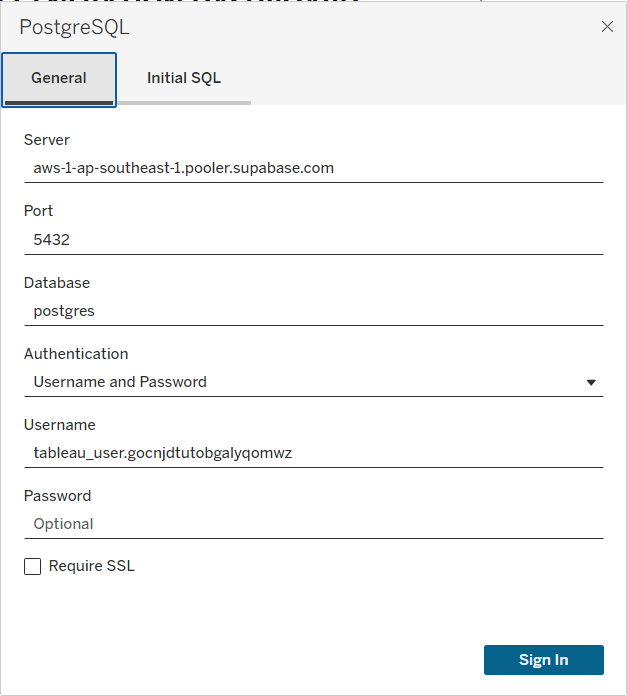
\includegraphics[width=0.62\textwidth]{figures/tableau_connect_supabase.png}
    
    
    \caption{Cấu hình kết nối PostgreSQL từ Tableau tới Supabase}
    \label{fig:tableau_connect_supabase}
\end{figure}

Thông số cấu hình kết nối chi tiết giữa Tableau và hệ cơ sở dữ liệu PostgreSQL của dự án được chuẩn hóa như trong Bảng~\ref{tab:tableau_connection_params}:

\begin{table}[H]
\centering
\caption{Thông số kết nối PostgreSQL từ Tableau tới Supabase}
\label{tab:tableau_connection_params}
\small
\renewcommand{\arraystretch}{1.25}
\begin{tabularx}{\textwidth}{@{} l l X @{}}
\toprule
\textbf{Tham số Kết nối} & \textbf{Giá trị Cấu hình} & \textbf{Ý nghĩa Kỹ thuật \& Bảo mật} \\
\midrule
\textbf{Connector Type} & PostgreSQL & Trình kết nối hiệu năng cao tối ưu hóa riêng cho PostgreSQL/Tableau. \\
\textbf{Server / Host} & \texttt{aws-1-ap-southeast-1.\allowbreak pooler.supabase.com} & Cổng Supabase Connection Pooler (AWS Singapore) giúp duy trì kết nối ổn định và tái sử dụng connection pool. \\
\textbf{Port} & \texttt{5432} / \texttt{6543} & Cổng \texttt{5432} (Session Mode) dành cho tiến trình Python ETL backend; cổng \texttt{6543} (Transaction Mode Pooler) dành cho Tableau Desktop. \\
\textbf{Database} & \texttt{postgres} & Cơ sở dữ liệu đích chứa các schema \texttt{bi\_mart}, \texttt{gold}, \texttt{dim}. \\
\textbf{Authentication} & Username and Password & Xác thực danh tính người dùng bằng phương thức mã hóa định danh. \\
\textbf{Username} & \texttt{tableau\_user.gocnjdtutobgalyqomwz} & Tài khoản dịch vụ chuyên dụng (Dedicated Service Account) được phân quyền Read-only tối thiểu (Principle of Least Privilege) trên schema \texttt{bi\_mart}. \\
\textbf{Encryption} & Require SSL / TLS & Bắt buộc mã hóa toàn bộ luồng truyền tải dữ liệu giữa máy trạm BI và máy chủ Supabase. \\
\bottomrule
\end{tabularx}


\end{table}

Việc sử dụng cổng Pooler kết hợp tài khoản dịch vụ phân quyền độc lập mang lại 3 ưu điểm kỹ thuật:
\begin{enumerate}[label=\arabic*., leftmargin=*]
    \item \textbf{Khả năng Chịu tải Cao (Concurrency Handling):} Cơ chế Connection Pooling tự động điều phối hàng trăm truy vấn phân tích song song từ các Dashboard mà không làm tràn bộ nhớ RAM của cụm máy chủ Supabase.
    \item \textbf{Bảo mật Dữ liệu Nghiêm ngặt (Least Privilege):} Tài khoản \texttt{tableau\_user} chỉ được cấp quyền \texttt{SELECT} trên tầng BI Mart và các bảng Dimension, ngăn chặn hoàn toàn rủi ro can thiệp thay đổi cấu trúc bảng hoặc ghi đè dữ liệu.
    \item \textbf{Độ trễ Truy vấn Cực thấp (Low Latency):} Cụm máy chủ đặt tại Datacenter Singapore (\texttt{ap-southeast-1}) đảm bảo thời gian phản hồi truy vấn dưới 1,5 giây cho mọi thao tác lọc tương tác từ Việt Nam.
\end{enumerate}

\subsection{Mô hình Kết nối Dữ liệu Tầng BI Mart và Tableau Relationships}
\label{subsec:bi_mart_model}

Để đảm bảo tốc độ phản hồi tính toán thời gian thực trên Tableau mà không gây quá tải cho hệ quản trị cơ sở dữ liệu Supabase PostgreSQL, dự án không thực hiện truy vấn trực tiếp trên các bảng sự kiện thô 2,7 triệu dòng. Thay vào đó, hệ thống Tableau kết nối trực tiếp với tầng BI Mart đã được tối ưu hóa sẵn thông qua hai Materialized Views lõi:
\begin{itemize}
    \item \texttt{bi\_mart.\allowbreak mv\_bi\_mart\_hourly\_measures}: Lưu trữ toàn bộ các đo lường chi tiết theo từng giờ của 42 trạm phát, bao gồm sản lượng thực tế (\texttt{e\_hourly}), sản lượng chuẩn STC (\texttt{e\_stc\_hourly}), sản lượng kỳ vọng hiệu chỉnh nhiệt (\texttt{e\_expected}), hệ số hiệu suất (\texttt{pr\_actual}, \texttt{pr\_adjusted}), suy hao do nhiệt (\texttt{loss\_temp}), nhiệt độ ô pin (\texttt{t\_cell}), cùng các cờ báo động ngoại lai GMM-IF (\texttt{gmm\_if\_outlier\_flag}).
    \item \texttt{bi\_mart.\allowbreak mv\_bi\_mart\_daily\_kpis}: Lưu trữ các chỉ số tổng hợp cấp ngày, tích hợp sẵn các chỉ số lũy kế theo tuần (\texttt{wtd\_energy}), tháng (\texttt{mtd\_energy}), năm (\texttt{ytd\_energy}), doanh thu ước tính (\texttt{daily\_revenue}), chi phí tổn thất do thiếu hụt công suất (\texttt{cost\_of\_underperformance}), và lượng phát thải khí nhà kính giảm thiểu (\texttt{daily\_co2\_avoided}).
\end{itemize}

Các Materialized Views này kết nối logic với hệ thống các bảng chiều (\texttt{dim\_solar\_site}, \texttt{dim\_geography}, \texttt{dim\_date}, \texttt{dim\_weather\_type}) thông qua mô hình liên kết Tableau Relationships (1-N). Mô hình này bảo toàn ngữ cảnh phân tích đa chiều mà không làm nhân bản dòng dữ liệu (Fan-out problem), tối ưu hóa tốc độ tải trang dưới 2 giây cho mọi thao tác tương tác lọc và khoan sâu (Drill-down).

\subsection{Bảng màu Ngữ nghĩa và Nguyên tắc Thiết kế UI/UX}
\label{subsec:color_palette}

Giao diện hệ thống Dashboard trên Tableau được thiết kế theo tư duy hiện đại, tối giản (Minimalist \& Clean Layout) nhằm tối đa hóa tỷ số dữ liệu trên mực in (Data-Ink Ratio) và tuân thủ các quy luật nhận thức thị giác Gestalt. Toàn bộ hệ màu được chuẩn hóa theo cấu hình giao diện \texttt{tableau\_theme.json} và ánh xạ trực tiếp từ tệp Workbook \texttt{main\_fixed\_01.twb}, đảm bảo độ tương phản cao ($\ge 4.5:1$) theo tiêu chuẩn WCAG 2.1 AA.

\subsubsection{Hệ thống Bảng màu Đồng bộ (Color Palette System)}

Nhằm phân biệt rõ ràng giữa các luồng thông tin vận hành và trạng thái kỹ thuật, hệ màu trong Dashboard được chia thành 3 phân nhóm chức năng: Bảng màu Chủ đạo (Primary), Bảng màu Cảnh báo Ngữ nghĩa (Semantic Alert), và Dải màu Tuần tự cho Heatmap (Sequential Palette).

\begin{table}[H]
\centering
\caption{Quy chuẩn bảng màu trong Tableau Workbook \texttt{main\_fixed\_01.twb}}
\label{tab:tableau_color_system}
\small
\renewcommand{\arraystretch}{1.3}
\begin{tabularx}{\textwidth}{@{} l l c X @{}}
\toprule
\textbf{Nhóm chức năng} & \textbf{Tên màu \& Mã Hex} & \textbf{Mẫu màu} & \textbf{Chỉ số \& Thành phần Ứng dụng trong Workbook} \\
\midrule
\multirow{3}{*}{\textbf{Bảng màu Chủ đạo}} 
& Classic Blue (\texttt{\#4E79A7}) & \textcolor{tblNavy}{\rule{1.2cm}{0.3cm}} & BANs sản lượng, đường xu hướng sản lượng thực tế ($e_{\text{hourly}}$), thanh Header. \\
& Solar Orange (\texttt{\#F28E2B}) & \textcolor{tblOrange}{\rule{1.2cm}{0.3cm}} & Bức xạ sóng ngắn (\texttt{shortwave\_radiation}), nhiệt độ môi trường, đường nhiệt ô pin. \\
& Eco Green (\texttt{\#59A14F}) & \textcolor{tblGreen}{\rule{1.2cm}{0.3cm}} & Hệ số công suất (Capacity Factor CF), thanh sản lượng lũy kế WTD/MTD/YTD. \\
\midrule
\multirow{4}{*}{\textbf{Cảnh báo Ngữ nghĩa}}
& Active/Success (\texttt{\#59A14F}) & \textcolor{tblGreen}{\rule{1.2cm}{0.3cm}} & Trạng thái tối ưu: $PR \ge 75\%$, tỷ lệ hoàn thành kế hoạch $\text{Yield Ratio} \ge 100\%$. \\
& Warning (\texttt{\#EDC948}) & \textcolor{tblYellow}{\rule{1.2cm}{0.3cm}} & Cảnh báo suy giảm nhẹ ($50\% \le PR < 75\%$), nhiệt độ ô pin vượt ngưỡng tối ưu $25^\circ\text{C}$. \\
& Danger/Outlier (\texttt{\#E15759}) & \textcolor{tblRed}{\rule{1.2cm}{0.3cm}} & Đánh dấu cờ bất thường GMM-IF, vết rò rỉ điện ban đêm ($E > 0$), sụt giảm nặng. \\
& Adjusted/Ref (\texttt{\#76B7B2}) & \textcolor{tblTeal}{\rule{1.2cm}{0.3cm}} & Đường hiệu suất hiệu chỉnh nhiệt ($PR_{\text{adjusted}}$), sản lượng kỳ vọng ($E_{\text{expected}}$). \\
\midrule
\multirow{2}{*}{\textbf{Dải màu Phân tích}}
& Sequential Heatmap & \textcolor{tblSeqWarm}{\rule{1.2cm}{0.3cm}} & Dải màu \texttt{orange\_10\_0} chuyển từ Vàng nhạt (\texttt{\#F9E9E0}) sang Đỏ (\texttt{\#E15759}) trên Heatmap. \\
& Neutral Gray (\texttt{\#79706E}) & \textcolor{tblGray}{\rule{1.2cm}{0.3cm}} & Đường chuẩn tham chiếu (Reference Lines), trục tọa độ, nhãn thông số phụ trợ. \\
\bottomrule
\end{tabularx}


\end{table}

\subsubsection{Nguyên tắc Bố cục Thị giác và Cấu trúc Khung Thẻ (Card-Based Container Layout)}

Bên cạnh hệ thống màu sắc, trải nghiệm tương tác trên Dashboard được tối ưu hóa thông qua các nguyên tắc thiết kế:
\begin{itemize}[noitemsep]
    \item \textbf{Cấu trúc Phân tầng F-Pattern:} Mắt người dùng tự nhiên quét từ góc trên bên trái sang phải và xuống dưới. Do đó, các thẻ chỉ số cốt lõi (BANs) như \texttt{KPI total gen}, \texttt{AVG CF}, \texttt{KPI PR} được đặt tại dải trên cùng (Top Banner) với kích thước chữ lớn (18--24pt) để người quản lý nắm bắt nhanh tình trạng hệ thống chỉ trong vài giây đầu tiên.
    \item \textbf{Bố cục Khung Thẻ Phân Khu (Card-Based Container Layout):} Bố cục trực quan của dự án sử dụng các khung thẻ container riêng biệt có viền xám nhẹ thanh lịch (\texttt{\#E2E8F0}) trên nền sáng để nhóm các thành phần phân tích có liên quan về mặt logic (Khối thẻ KPI tổng hợp, Khối phân bố địa lý theo khuôn viên, Khối biểu đồ chuỗi thời gian sản lượng, Khối ma trận nhiệt tổn thất và Bảng xếp hạng thiết bị biến tần). Việc phân định bằng khung viền thẻ giúp người dùng dễ dàng định vị các vùng thông tin chức năng mà không bị rối mắt.
    \item \textbf{Tối ưu hóa Tỷ lệ Mực Thông tin (Data-Ink Ratio):} Bên trong mỗi thẻ biểu đồ, các đường lưới phụ (minor gridlines) được làm mờ hoặc loại bỏ, chỉ giữ lại các mốc tọa độ chính yếu và đường gốc (Zero-line) với tông màu xám rất nhạt (\texttt{\#E0E0E0}), giúp mắt người xem tập trung tối đa vào hình dáng biến thiên của đường cong sản lượng và các điểm dị thường nổi bật.
    \item \textbf{Đồng bộ Bộ lọc Toàn cục (Synchronized Global Filtering):} Toàn bộ bộ lọc theo Trạm (\texttt{Site Name}), Khoảng thời gian (\texttt{Date Range}), và Loại thời tiết (\texttt{Weather Type}) được bố trí gọn gàng tại bảng điều khiển bên phải (Right-panel) dưới dạng Dropdown, tự động đồng bộ hóa trên toàn bộ 3 Dashboard.
\end{itemize}

\subsection{Các Trường Tính toán Nghiệp vụ Bổ sung trên Tableau (Calculated Fields)}
\label{subsec:calculated_fields}

Để đáp ứng các yêu cầu phân tích kinh doanh đa chiều và các biểu đồ trực quan động trên Tableau, nhóm đã thiết lập một hệ sinh thái các Trường tính toán (Calculated Fields) chuyên sâu trong tệp tin \texttt{main\_fixed\_01.twb}. Bảng~\ref{tab:tableau_calculated_fields} tổng hợp các công thức tính toán nghiệp vụ cốt lõi:

\begin{table}[H]
\centering
\caption{Tổng hợp các trường tính toán nghiệp vụ trên Tableau}
\label{tab:tableau_calculated_fields}
\small
\renewcommand{\arraystretch}{1.25}
\begin{tabularx}{\textwidth}{@{} >{\raggedright\arraybackslash}p{3.2cm} >{\raggedright\arraybackslash\ttfamily\scriptsize}p{6.0cm} >{\raggedright\arraybackslash}X @{}}
\toprule
\textbf{Tên Trường} & \textbf{Công thức Tableau} & \textbf{Ý nghĩa Nghiệp vụ} \\
\midrule
\texttt{[PR Actual]} & 
SUM(IF [shortwave\_radiation] >= 100 \newline
\quad AND [p\_stc] > 0 THEN [e\_hourly] END) \newline
/ SUM(IF [shortwave\_radiation] >= 100 \newline
\quad AND [p\_stc] > 0 \newline
\quad THEN [capacity\_kw] * ([shortwave\_radiation] / 1000.0) END) & 
Tính toán Hệ số Hiệu suất (PR) thực tế có điều kiện, loại bỏ các khoảng thời gian bức xạ yếu dưới $100\,\text{W/m}^2$ khi biến tần chưa phát điện. \\
\midrule
\texttt{[Weighted CF Trend]} & 
SUM([e\_hourly]) / SUM([p\_stc]) & 
Hệ số công suất gia quyền theo tổng quy mô lắp đặt, phản ánh mức độ huy động công suất thực tế của toàn trạm. \\
\midrule
\texttt{[Number of Inverter]} & 
IF CONTAINS(LOWER([inverter]), 'x') \newline
THEN INT(TRIM(SPLIT(LOWER([inverter]), 'x', 1))) \newline
ELSE 1 END & 
Tách số lượng biến tần từ chuỗi văn bản kỹ thuật (ví dụ: \texttt{2x Fronius Symo 20.0}). \\
\midrule
\texttt{[kWh/inverter]} & 
[e\_hourly] / [Number of Inverter] & 
Sản lượng chuẩn hóa trên mỗi đầu biến tần, hỗ trợ so sánh hiệu quả giữa các dòng thiết bị. \\
\midrule
\texttt{[kWh/panel]} & 
[e\_hourly] / [number\_of\_panels] & 
Sản lượng trung bình trên mỗi tấm pin, hỗ trợ nhận diện các chuỗi pin bị che bóng hoặc suy thoái. \\
\midrule
\texttt{[Outlier Hours SM/PM]} & 
SUM(IF MONTH([full\_date]) = [Param Month] \newline
\quad AND [gmm\_if\_outlier\_flag] = TRUE \newline
\quad THEN 1 ELSE 0 END) & 
Tính tổng số giờ xuất hiện dị thường trong tháng được chọn (SM) và tháng liền kề trước đó (PM). \\
\midrule
\texttt{[Outlier Hours MoM \%]} & 
([Outlier Hours SM] - [Outlier Hours PM]) \newline
/ ZN([Outlier Hours PM]) & 
Tốc độ tăng trưởng số giờ dị thường theo tháng (Month-over-Month), phản ánh mức độ gia tăng sự cố vận hành. \\
\midrule
\texttt{[Outlier MoM \% (Up/Down)]} & 
IF [Outlier Hours MoM \%] > 0 \newline
THEN [Outlier Hours MoM \%] END & 
Phân nhánh điều kiện để gán màu trực quan (màu đỏ khi sự cố tăng, màu xanh khi sự cố giảm) trên thẻ KPI. \\
\bottomrule
\end{tabularx}

\end{table}

\subsection{Khung 3 Biến thể PR (IEC 61724-1) và Cơ chế Phòng chống Lỗi Ô nhiễm Đường Cơ sở}
\label{subsec:pr_triple_metrics}

Hệ số Hiệu suất (Performance Ratio -- PR) là thước đo chất lượng vận hành quan trọng nhất của trạm quang điện. Tuy nhiên, nếu chỉ sử dụng một công thức $PR$ thô duy nhất, nhà quản lý sẽ dễ bị đánh lừa bởi biến động thời tiết hoặc rơi vào bẫy logic vòng lặp (Circular Logic). Dự án thiết lập Khung 3 Biến thể PR chuẩn hóa theo tiêu chuẩn quốc tế IEC 61724-1:

\begin{enumerate}[label=\arabic*., leftmargin=*]
    \item \textbf{1. $PR_{\text{actual}}$ (Nominal PR -- Đo đạc thực tế):}
    \begin{equation}
        PR_{\text{actual}} = \frac{\sum E_{\text{actual}}}{\sum \left[ P_{\text{stc}} \cdot \left(\frac{GHI}{1000\,\text{W/m}^2}\right) \cdot \Delta t \right]} \times 100\%
    \end{equation}
    Để loại trừ sai số góc nghiêng cảm biến pyranometer vào sáng sớm/chiều tà và điện áp chưa đạt ngưỡng khởi động biến tần, hệ thống Tableau tự động áp dụng bộ lọc điều kiện: chỉ tính toán $PR_{\text{actual}}$ khi $GHI \ge 100\,\text{W/m}^2$.

    \item \textbf{2. $PR_{\text{corr}}$ (Temperature-Corrected PR -- Chuẩn hóa nhiệt độ cell theo IEC 61724-1 Annex B):}
    \begin{equation}
        PR_{\text{corr}} = \frac{PR_{\text{actual}}}{1 + \gamma \cdot (T_{\text{cell}} - 25^\circ\text{C})}
    \end{equation}
    với $\gamma = -0{,}38\%/^\circ\text{C}$. Biến thể này bù trừ toàn bộ ảnh hưởng của nhiệt độ môi trường, đưa hiệu suất về mốc chuẩn phòng thí nghiệm $25^\circ\text{C}$. Nhờ đó, đường xu hướng $PR_{\text{corr}}$ qua nhiều năm giúp kỹ sư O\&M phát hiện chính xác mức độ thoái hóa phần cứng tự nhiên ($< 0{,}5\%/\text{năm}$) mà không bị nhiễu bởi các đợt sóng nhiệt mùa hè.

    \item \textbf{3. $PR_{\text{adjusted}}$ (Adjusted Benchmark PR -- Đường chuẩn kỳ vọng trong BI Mart):}
    \begin{equation}
        T_{\text{cell}} = T_{\text{ambient}} + (GHI \times 0{,}03)
    \end{equation}
    \begin{equation}
        Loss_{\text{temp}} = 0{,}0038 \times \max(0, T_{\text{cell}} - 25^\circ\text{C})
    \end{equation}
    \begin{equation}
        PR_{\text{adjusted}} = 0{,}85 \times (1 - Loss_{\text{temp}})
    \end{equation}
\end{enumerate}

\textbf{Luận cứ Khoa học Phân rã Hằng số Thiết kế 0,85 và Phòng chống Ô nhiễm Đường Cơ sở:}

Điểm then chốt trong công thức $PR_{\text{adjusted}}$ là việc sử dụng hệ số thiết kế danh định STC $\mathbf{0{,}85}$ thay vì tính toán dựa trên dữ liệu lịch sử đo đạc của chính trạm đó. Con số $0{,}85$ phản ánh hiệu suất cân bằng hệ thống danh định ($\eta_{\text{BOS, nominal}} = 100\% - 15\% = 0{,}85$) ở điều kiện phòng thí nghiệm ($25^\circ\text{C}$), được cấu thành từ $15\%$ tổng tổn thất phần cứng cố định theo các chuẩn mực kỹ thuật quốc tế (NREL PVWatts, IEC 61724-1 và mô hình thiết kế PVsyst) như chi tiết tại Bảng~\ref{tab:bos_derate_breakdown}:

\begin{table}[H]
\centering
\caption{Phân rã các thành phần tổn thất hệ thống cố định cấu thành hằng số thiết kế $\eta_{\text{BOS}} = 0{,}85$}
\label{tab:bos_derate_breakdown}
\small
\renewcommand{\arraystretch}{1.25}
\begin{tabularx}{\textwidth}{@{} l >{\raggedright\arraybackslash}p{4.8cm} c X @{}}
\toprule
\textbf{STT} & \textbf{Hạng Mục Tổn Thất Phần Cứng (BOS)} & \textbf{Tỷ Lệ (\%)} & \textbf{Cơ Sở Kỹ Thuật \& Tiêu Chuẩn Tham Chiếu} \\
\midrule
1 & Hiệu suất chuyển đổi Biến tần (Inverter DC/AC) & $2{,}50\%$ & Hiệu suất châu Âu (Euro-efficiency) của các dòng Inverter Fronius Symo / SMA đạt $97{,}50\%$. \\
2 & Sụt áp trở kháng dây dẫn DC (DC Ohmic Loss)     & $1{,}50\%$ & Tổn thất phát nhiệt trên tuyến cáp từ dàn pin đến tủ gom DC theo chuẩn AS/NZS 5033. \\
3 & Tổn thất truyền tải AC \& Máy biến áp            & $1{,}00\%$ & Trở kháng cáp đồng AC từ ngõ ra biến tần tới tủ phân phối chính và đồng hồ đo. \\
4 & Sai lệch Module \& Dung sai chế tạo (Mismatch)   & $1{,}50\%$ & Sai lệch đường đặc tính I-V giữa các tấm pin trong cùng chuỗi nối tiếp và dung sai xuất xưởng ($\pm 3\%$). \\
5 & Suy thoái quang học ban đầu (LID)               & $1{,}50\%$ & Hiện tượng suy giảm phân rã do ánh sáng (Light-Induced Degradation) của tế bào silicon P-type. \\
6 & Phản xạ góc tới bề mặt kính (IAM Reflection)    & $2{,}50\%$ & Tổn thất tán xạ quang học bề mặt kính (Incidence Angle Modifier) khi góc chiếu lệch tâm. \\
7 & Bụi mỏng nền \& Che bóng kết cấu vi mô           & $4{,}50\%$ & Lớp bụi mỏng tự nhiên không thể rửa trôi hoàn toàn ($2{,}0\%$) và góc khuất gờ nhôm/lan can ($2{,}5\%$). \\
\midrule
\multicolumn{2}{l}{\textbf{Tổng tổn thất hệ thống cố định ($\sum Loss_{\text{BOS}}$)}} & $\mathbf{15{,}00\%}$ & $\mathbf{\eta_{\text{BOS, nominal}} = 100\% - 15{,}00\% = 0{,}8500}$ \\
\bottomrule
\end{tabularx}
\end{table}

Phần tổn thất do nhiệt độ ô pin ($Loss_{\text{temp}}$) không nằm trong con số $15\%$ cố định này vì nó biến thiên động học liên tục theo từng mốc quan trắc thời tiết. Do đó, mô hình tách riêng thành thừa số hiệu chỉnh thời gian thực: $PR_{\text{adjusted}} = 0{,}85 \times (1 - Loss_{\text{temp}})$.

\textbf{Cơ chế Phòng chống Lỗi Ô nhiễm Đường Cơ sở (Baseline Contamination):}
Nếu tính đường chuẩn từ trung bình $PR_{\text{actual}}$ trong quá khứ của trạm, khi một trạm bị hỏng hóc nghiêm trọng (ví dụ: đứt cầu chì chuỗi pin khiến $PR_{\text{actual}}$ sụt xuống $35\%$), đường cơ sở sẽ bị ``ô nhiễm'' (Baseline Contamination) và tự động kéo tụt mốc kỳ vọng xuống thấp theo. Khi đó, tỷ lệ hoàn thành kế hoạch ($\text{Yield Ratio} = E_{\text{actual}} / E_{\text{expected}}$) vẫn báo cáo trạm đạt $100\%$ hiệu năng, khiến hệ thống giám sát bị ``mù'' trước các sự cố phần cứng kéo dài (Lỗi vòng lặp logic -- Circular Logic). Việc cố định mốc thiết kế $0{,}85$ kết hợp bù nhiệt động học bảo đảm $PR_{\text{adjusted}}$ luôn là một thước đo tham chiếu khách quan tuyệt đối.

\section{Chi tiết Hệ thống Dashboard Phân tích trên Tableau Desktop}
\label{sec:dashboard_details}

Hệ thống trực quan hóa của dự án được đóng gói hoàn chỉnh trong tệp tin Tableau Workbook \texttt{reports/dashboards/\allowbreak main\_fixed\_01.twb}, bao gồm 3 Dashboard chuyên biệt được kết nối chặt chẽ theo luồng phân tích nguyên nhân - kết quả.

\subsection{Dashboard 1: Executive Overview (Tổng quan Vận hành)}
\label{subsec:db_overview}

Dashboard \textit{Executive Overview} đóng vai trò là trung tâm chỉ huy dành cho Ban Giám đốc và các nhà quản lý dự án, cung cấp bức tranh toàn cảnh về sản lượng, doanh thu và sức khỏe vận hành của toàn bộ 42 trạm điện mặt trời tại Úc.

\begin{figure}[H]
    \centering
    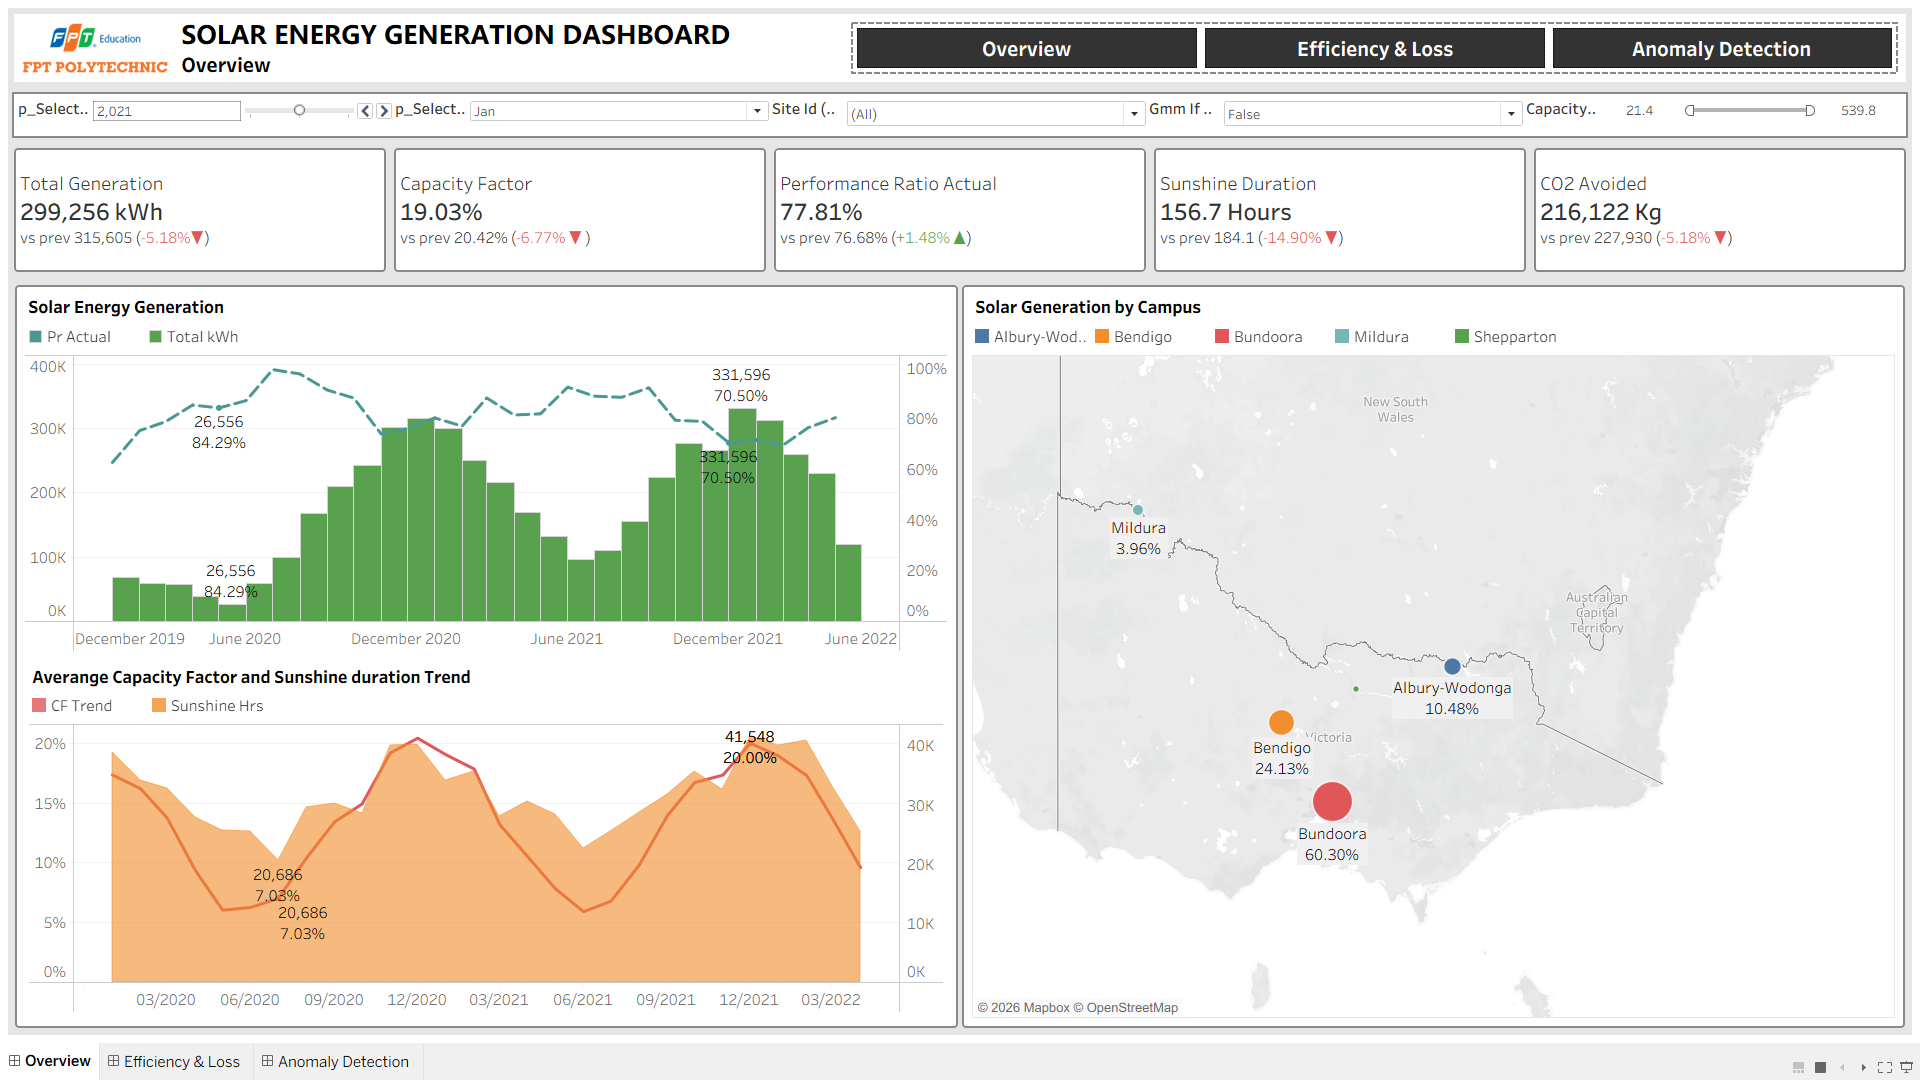
\includegraphics[width=0.95\textwidth]{figures/Dashboard_overview.png}
    
    
    \caption{Giao diện Dashboard 1: Tổng quan điều hành (Executive Overview)}
    \label{fig:dashboard_overview}
\end{figure}

Các thành phần giao diện và chỉ số phân tích chính bao gồm:
\begin{enumerate}[label=\alph*., leftmargin=*]
    \item \textbf{Thẻ Chỉ số Cốt lõi (BANs Layer):}
    \begin{itemize}
        \item \texttt{KPI total gen}: Hiển thị tổng sản lượng điện phát lũy kế ($E_{\text{actual}}$) tính bằng MWh/GWh, tích hợp so sánh tốc độ tăng trưởng MoM/YoY.
        \item \texttt{AVG CF}: Hệ số công suất khai thác trung bình ($\text{Capacity Factor} = \sum E / (P_{\text{stc}} \cdot 24)$).
        \item \texttt{KPI PR \& PR adjust}: Chỉ số hiệu suất thực tế ($PR_{\text{actual}}$) và chỉ số hiệu suất đã hiệu chỉnh nhiệt độ ($PR_{\text{adjusted}}$).
        \item \texttt{KPI Co2 avoided \& Sunshine dur}: Tổng khối lượng khí thải $\text{CO}_2$ triệt tiêu (kg), số cây xanh tương đương được trồng mới và tổng thời lượng nắng tích tụ trong kỳ.
    \end{itemize}

    \item \textbf{Bản đồ Địa lý Phân bố Trạm (Campus Map):}
    Trực quan hóa vị trí địa lý thực tế của 42 trạm PV tại các cơ sở đào tạo (Campus). Kích thước hình tròn (Symbol size) đại diện cho công suất thiết kế ($P_{\text{stc}}$ tính bằng $kWp$), trong khi màu sắc (Color gradient) phản ánh trực tiếp hệ số công suất CF. Nhờ đó, người quản lý lập tức nhận diện được các vùng địa lý có hiệu suất khai thác kém bất thường.

    \item \textbf{Ma trận Hiệu suất Trạm (Site Performance Matrix \& Consistency):}
    Biểu đồ xếp hạng phân bổ sản lượng ($gen/panel$) và độ ổn định vận hành giữa 42 trạm. Hệ thống trực quan hóa sự chênh lệch sản lượng trên từng tấm pin, giúp phát hiện các trạm đang hoạt động dưới mức tiềm năng thiết kế.

    \item \textbf{Xu hướng Sản lượng Tổng hợp (Total Generation \& Trend):}
    Biểu đồ đường/miền (Line/Area Chart) thể hiện sự biến đổi sản lượng theo thời gian (ngày, tháng) kết hợp phân tích đóng góp sản lượng theo từng chủng loại tấm pin (Panel Brands/Models).
\end{enumerate}

\subsection{Dashboard 2: Operational Efficiency \& Loss Analysis (Hiệu suất Vận hành \& Phân rã Tổn thất)}
\label{subsec:db_efficiency}

Dashboard \textit{Efficiency \& Loss} được thiết kế dành riêng cho đội ngũ kỹ sư kỹ thuật năng lượng nhằm ``giải thích'' nguyên nhân gốc rễ gây sụt giảm sản lượng, đặc biệt là hiện tượng suy hao do nhiệt độ (Thermal Degradation) và hiệu suất biến tần (Inverter/Optimizer).

\begin{figure}[H]
    \centering
    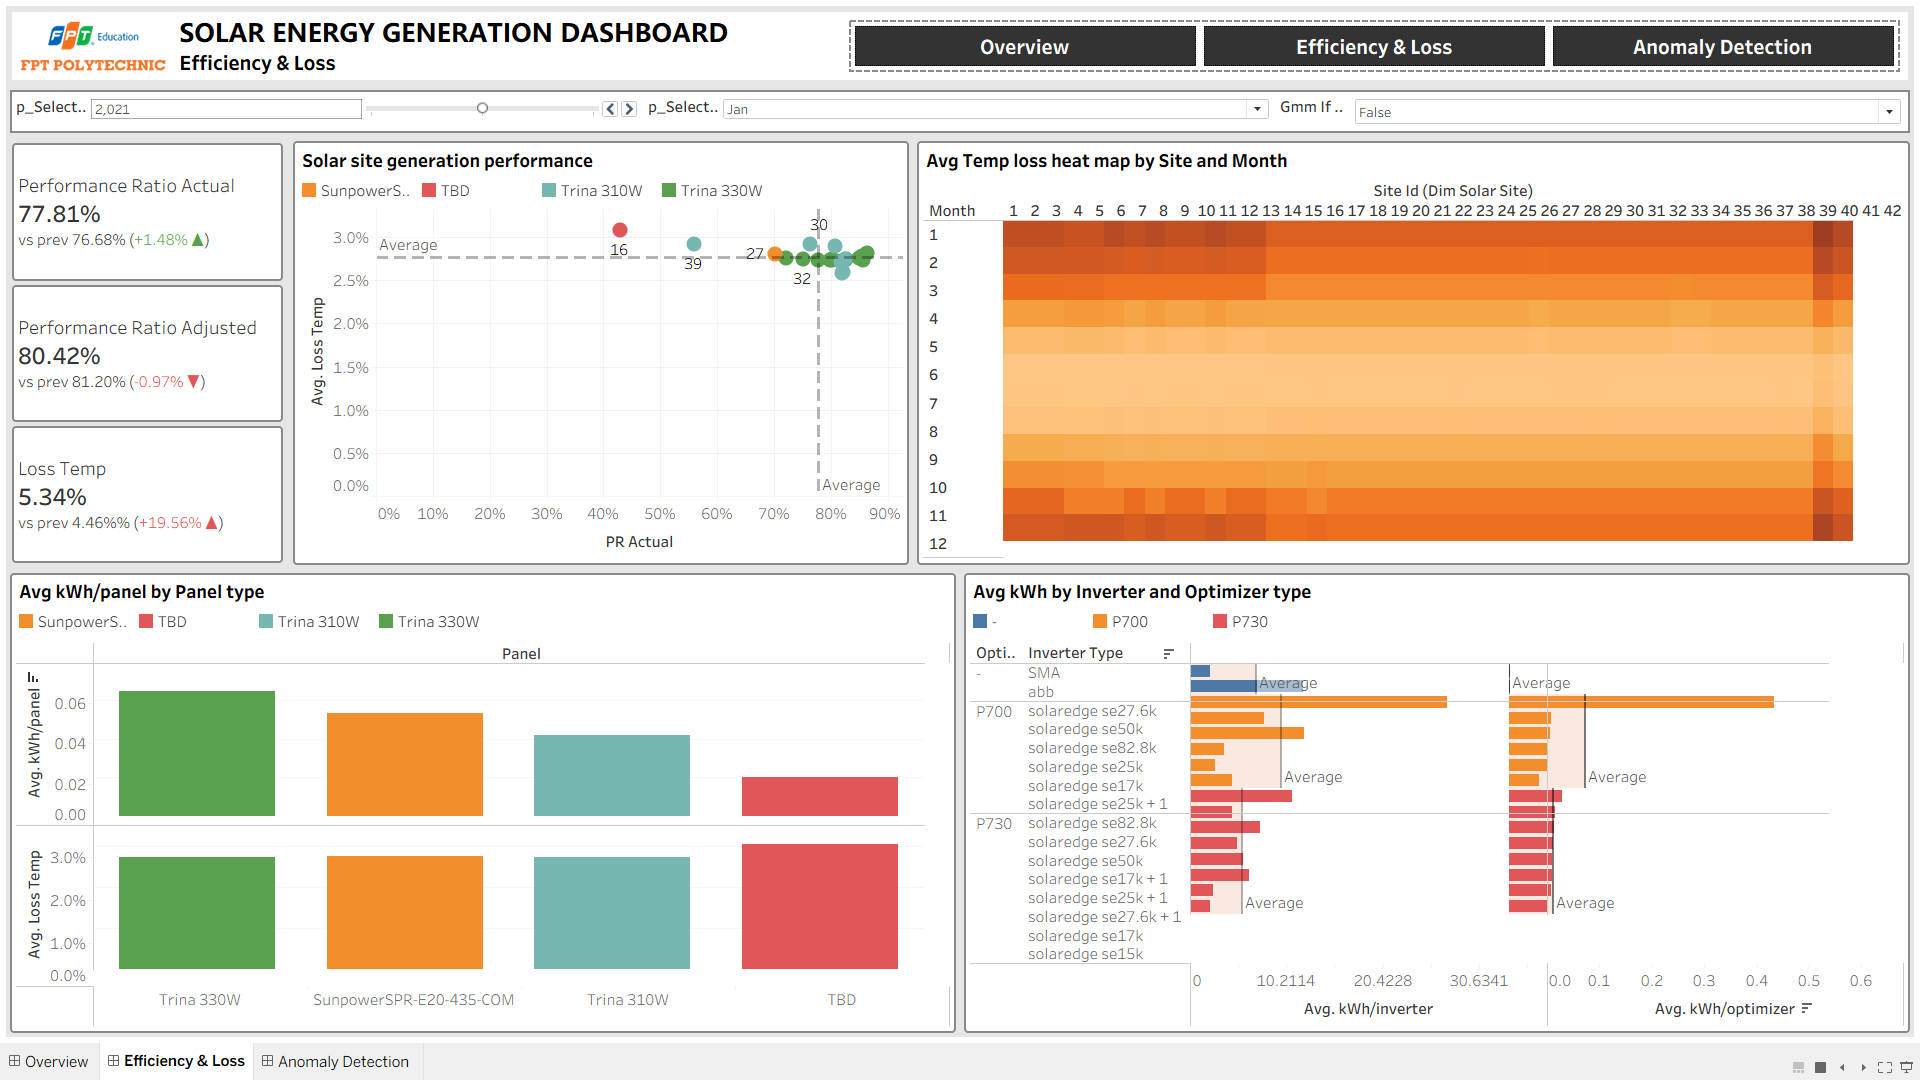
\includegraphics[width=0.95\textwidth]{figures/dashboard_efficiency_and_loss.png}
    
    
    \caption{Giao diện Dashboard 2: Hiệu suất và tổn thất vận hành}
    \label{fig:dashboard_efficiency}
\end{figure}

Các phân tích kỹ thuật trên Dashboard bao gồm:
\begin{enumerate}[label=\alph*., leftmargin=*]
    \item \textbf{Đồ thị Xu hướng Tổn thất Nhiệt (Generation \& Loss Trend):}
    Sử dụng biểu đồ 2 trục tọa độ độc lập (Dual-Axis Chart) kết hợp giữa Sản lượng điện thực tế ($e_{\text{hourly}}$), Bức xạ sóng ngắn mặt trời (\texttt{shortwave\_radiation}) và Nhiệt độ ô pin ($T_{\text{cell}}$). Biểu đồ chứng minh luận điểm kỹ thuật quan trọng: Vào các khung giờ giữa trưa khi bức xạ đạt đỉnh cực đại ($> 800 \, \text{W/m}^2$), nhiệt độ ô pin tăng cao vượt quá $45^\circ\text{C}$ làm đường cong sản lượng bị chững lại hoặc suy giảm đáng kể so với mức lý thuyết.

    \item \textbf{Lưới Nhiệt Suy hao Nhiệt độ (Temperature Loss Heatmap \& Loss by Month):}
    Bản đồ nhiệt (Heatmap) thể hiện tỷ lệ tổn thất nhiệt độ trung bình (\texttt{avg\_loss\_temp}) phân rã theo 12 tháng trong năm và theo từng trạm phát. Dải màu chuyển từ Vàng nhạt (tổn thất $< 3\%$) sang Đỏ thẫm (tổn thất $> 8\%$), chỉ ra chính xác các tháng mùa hè đỉnh điểm cần tăng cường giải pháp làm mát hoặc thông gió bề mặt pin.

    \item \textbf{Đánh giá Hiệu suất Thiết bị (Inverter \& Optimizer Efficiency Rank):}
    Trực quan hóa chỉ số sản lượng trung bình trên mỗi tấm pin ($kWh/panel$) và tỷ lệ đáp ứng sản lượng kỳ vọng (\texttt{Yield ratio} $= E_{\text{actual}} / E_{\text{expected}}$) phân loại theo các hãng chế tạo Inverter và Optimizer. Phân tích này hỗ trợ đội ngũ bảo trì đánh giá chất lượng thiết bị vật lý thực tế để đưa ra quyết định thay thế hoặc bảo hành linh kiện.
\end{enumerate}

\subsection{Dashboard 3: Anomaly Detection \& Predictive Maintenance (Giám sát Bất thường \& Bảo trì Cảnh báo)}
\label{subsec:db_anomaly}

Dashboard \textit{Anomaly Detection} đóng vai trò là hệ thống cảnh báo sớm (Early Warning System) cho đội ngũ O\&M, trực quan hóa toàn bộ các cờ bất thường được phát hiện từ mô hình học máy GMM-IF và thuật toán Rolling IQR.

\begin{figure}[H]
    \centering
    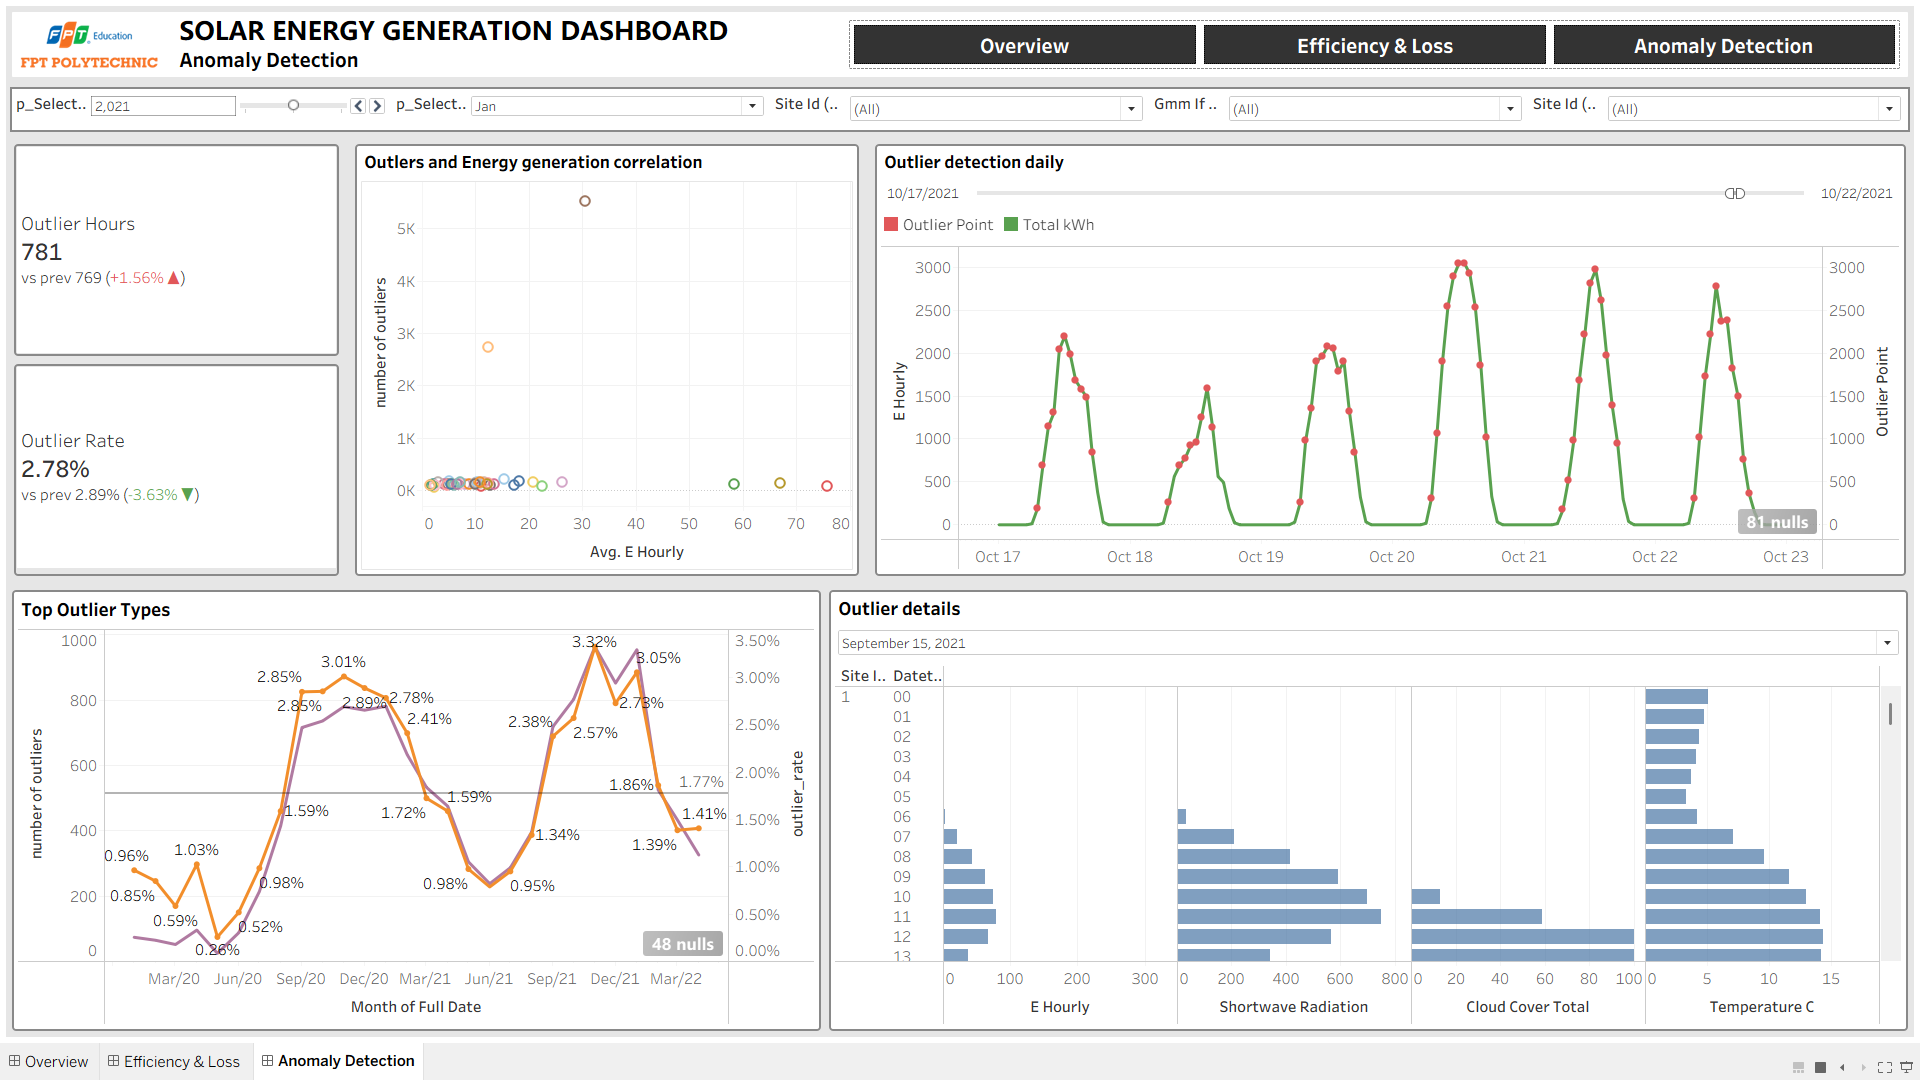
\includegraphics[width=0.95\textwidth]{figures/dashboard_anomaly_detection.png}
    
    
    \caption{Giao diện Dashboard 3: Giám sát dị thường và bảo trì dự đoán}
    \label{fig:dashboard_anomaly}
\end{figure}

Các tính năng giám sát bất thường trọng tâm bao gồm:
\begin{enumerate}[label=\alph*., leftmargin=*]
    \item \textbf{Thẻ Thống kê Bất thường (Anomaly KPIs):}
    Hiển thị tổng số giờ phát hiện bất thường (\texttt{KPI Outlier Hours}), tỷ lệ phần trăm dữ liệu dị thường (\texttt{KPI Outlier Rate}), số lượng bản ghi gắn cờ (\texttt{number of outliers}) và chỉ số biến động so với tháng trước (\texttt{Outlier Rate MoM \%}).

    \item \textbf{Biểu đồ Chuỗi thời gian Phát hiện Dị thường (Time-series Outlier Detect):}
    Đồ thị chuỗi thời gian liên tục 15 phút biểu diễn sản lượng điện. Tất cả các mốc thời gian bị mô hình GMM-IF gắn cờ bất thường (\texttt{gmm\_if\_outlier\_flag = true}) được đánh dấu bằng các điểm nút tròn màu Đỏ rực (\texttt{\#E15759}) trên nền đường line sản lượng. Kỹ sư có thể nhấp chuột trực tiếp vào điểm dị thường để mở thẻ thông tin chi tiết (Tooltip) hiển thị lý do bất thường (\texttt{gmm\_if\_outlier\_reason}).

    \item \textbf{Bản đồ Nhiệt Phát hiện Rò rỉ Điện Ban đêm (Outlier by Site Heatmap):}
    Bản đồ nhiệt 2 chiều với Trục tung đại diện cho 24 khung giờ trong ngày ($0 - 23h$) và Trục hoành đại diện cho 42 trạm phát. 
    
    Quy tắc trực quan hóa áp đặt điều kiện đặc biệt: Nếu trong khung giờ ban đêm từ 18:30 đến 05:30 xuất hiện giá trị sản lượng $E > 0$, ô tương ứng sẽ lập tức bị tô màu Đỏ đậm. Đây là bằng chứng trực quan trực tiếp phát hiện sự cố rò rỉ dòng điện ngược (Reverse Current) hoặc cảm biến đo đạc CT bị sai lệch mốc 0 (Zero-drift fault), giúp kỹ sư khoanh vùng vị trí sự cố ngay lập tức.

    \item \textbf{Chi tiết Cảnh báo Phân loại Lỗi (Outlier Type \& Details):}
    Bảng thống kê chi tiết danh sách trạm và phân loại nhóm nguyên nhân dị thường (\textit{Night Leakage}, \textit{Extreme Power Spike}, \textit{Sensor Freeze}, \textit{Daytime Sudden Drop}), hỗ trợ lập danh mục ưu tiên cho các đội kỹ thuật đi kiểm tra hiện trường.
\end{enumerate}

\newpage
% ── Tinh chinh float RIENG cho chuong Hoc may ──
\setcounter{topnumber}{3}
\setcounter{bottomnumber}{2}
\setcounter{totalnumber}{4}
\renewcommand{\topfraction}{0.92}
\renewcommand{\bottomfraction}{0.7}
\renewcommand{\textfraction}{0.06}
\renewcommand{\floatpagefraction}{0.85}

\chapter{Xây dựng và Đánh giá Mô hình Học máy Dự báo Sản lượng}
\label{chap:forecasting}

% Sinh tu Section6.tex - CHI phan than, khong preamble. Dung bang \input trong
% DATN_OUTLIERS_REPORT.tex. Sua noi dung thi sua Section6.tex roi sinh lai.
%
% KHONG dat \clearpage o day. Hoi Section6 con la tai lieu doc lap thi dong do hop ly,
% nhung trong ban ghep no no ngay SAU \chapter{...} nen day toan bo noi dung sang trang
% ke tiep, de tieu de chuong 7 nam tro mot minh tren mot trang trong.

\FloatBarrier
\section{Tổng quan quy trình học máy}

Mục này khoanh phạm vi qua năm bước: dữ liệu đầu vào, bài toán và hai tầm dự báo, nhãn
ngoại lai kế thừa từ tầng ETL, sơ đồ toàn cảnh, và năm rào chắn chống rò rỉ.

\FloatBarrier
\subsection{Phạm vi và dữ liệu đầu vào}

Phần này trình bày toàn bộ quy trình học máy của dự án, bắt đầu từ tệp dữ liệu đã
làm sạch ở tầng ETL và kết thúc ở ứng dụng dự báo.

Bản trích tầng ETL bàn giao là tệp \path{data/mlmart_base/v5_preprocessing.parquet},
gồm $2.731.946$ bản ghi ở độ phân giải $15$ phút, thu thập từ $42$ dàn quang điện
đặt tại $5$ khuôn viên của Đại học La Trobe, Úc. Mỗi bản ghi mang giá trị sản lượng
của một dàn tại một mốc thời gian, kèm các biến khí tượng tương ứng lấy từ Open-Meteo.
Không phải mọi giá trị đều là số đo gốc~--- cột \texttt{energy\_source} phân biệt dòng
đo thật với dòng do tầng ETL điền khuyết, và Mục~\ref{subsec:hien_trang_du_lieu} trình bày tỷ lệ từng loại.

Bản trích này còn $26$ cột mang ô khuyết, nên bước mở đầu của quy trình học máy là xử lý
khuyết cho nhóm siêu dữ liệu và nhóm biến khí tượng. Riêng \texttt{capacity\_kw} và
\texttt{number\_of\_panels} ($1.132.078$ dòng, tức $41{,}44\%$) được giữ nguyên khuyết:
$17/42$ trạm thiếu toàn bộ và bốn trong năm khuôn viên không có nổi một giá trị tham chiếu,
nên mọi phép điền đều là suy diễn không căn cứ, trong khi LightGBM xử lý ô khuyết trực tiếp.
Siêu dữ liệu dạng chữ được điền theo hai tầng. Tầng một lấy giá trị liền kề trong chính
trạm cho \texttt{panel}, \texttt{inverter}, \texttt{location\_name} và
\texttt{campus\_name}; tầng hai điền \texttt{Unknown} cho những trạm rỗng toàn bộ nên
tầng một không có gì để lấy. Riêng \texttt{optimizers} ($1.259.007$ dòng, tức
$46{,}08\%$) điền \texttt{None} và \texttt{site\_metric} điền \texttt{kWh}. Biến khí tượng ở đợt trích
này chỉ còn khuyết $218$ ô mỗi cột~--- phần khuyết lớn của \texttt{cloud\_cover\_low} và
\texttt{wind\_speed} các đợt trước đã được tầng ETL điền từ thượng nguồn~--- và được lấp
theo ba nấc nối tiếp: gán $0$ cho các mốc ban đêm, lấp tiến theo chính trạm với hạn mức
từ một đến ba giờ, rồi mới dùng trung vị theo cặp (trạm, giờ). Mỗi cột số
được điền đều kèm một cột cờ hậu tố \texttt{\_is\_imputed} để các bước sau còn phân biệt
được ô đo thật với ô suy ra~--- tổng cộng $7$ cột cờ.

Kết quả ghi ra \path{data/mlmart_base/v5_final_cleaned.parquet}: giữ nguyên
$2.731.946$ dòng, số cột tăng từ $47$ lên $54$, và số cột còn ô khuyết giảm từ $26$ xuống
$6$. Sáu cột còn khuyết gồm \texttt{gmm\_if\_outlier\_reason}~--- chỉ có giá trị ở dòng bị
gán nhãn ngoại lai nên khuyết là đúng bản chất~--- hai cột công suất
\texttt{capacity\_kw} và \texttt{number\_of\_panels} được giữ khuyết theo quyết định không
điền ở trên, cùng ba cột tham chiếu thời tiết
\texttt{weather\_id}, \texttt{weather\_timestamp} và \texttt{weather\_type\_is\_day}, mỗi
cột khuyết $218$ ô và không cột nào tham gia vào bộ đặc trưng của mô hình. Từ đây trở đi,
\path{v5_final_cleaned.parquet} là đầu vào duy nhất của mọi bước còn lại trong tài liệu này.

Phần sản lượng bắt nguồn từ bộ dữ liệu mở UNISOLAR do Wimalaratne và cộng
sự~\cite{wimalaratne2022unisolar} công bố. Bài báo mô tả đúng cấu hình mà dự án đang
dùng, $42$ vị trí lắp đặt điện mặt trời trên $5$ khuôn viên của Đại học La Trobe, bang Victoria,
Úc, đo ở bước $15$ phút, kèm vị trí địa lý và thông số kỹ thuật của từng vị trí lắp đặt.

UNISOLAR đi kèm dữ liệu khí tượng của Cục Khí tượng Úc ở bước $1$ phút. Dự án lấy biến
khí tượng từ Open-Meteo theo toạ độ của từng khuôn viên, nên mọi kết luận về
nhóm đặc trưng khí tượng trong tài liệu này thuộc về nguồn Open-Meteo.

Hai trạm mang số hiệu $19$ và $24$ có siêu dữ liệu công suất lắp đặt mâu thuẫn với
sản lượng đo được, nên bị loại khỏi phạm vi huấn luyện và chấm điểm. Mô hình cuối cùng
vì vậy được đánh giá trên $40$ trạm; hai trạm còn lại vẫn nằm trong kho dữ liệu và vẫn
hiển thị trên ứng dụng, chỉ không tham gia vào các con số được báo cáo.
\FloatBarrier
\subsection{Bài toán và tầm dự báo}

Mục tiêu dự báo là sản lượng điện phát ra của từng vị trí lắp đặt điện mặt trời, ký hiệu
$y$, đơn vị kWh trên mỗi khoảng $15$ phút. Đây là bài toán dự báo chuỗi thời gian có
biến ngoại sinh: ngoài lịch sử sản lượng của chính vị trí đó, mô hình còn được cung cấp
các biến khí tượng và hình học Mặt Trời (\textit{solar geometry}) tại thời điểm cần dự báo.

Tầm dự báo (\textit{forecast horizon}) là khoảng cách thời gian giữa thời
điểm đưa ra dự báo và thời điểm được dự báo. Dự án huấn luyện hai cấu hình ứng với hai
tầm:

\begin{itemize}
    \item \textbf{H1} --- dự báo sản lượng tại $T + 15$ phút. Dữ liệu ghi ở bước $15$ phút
    nên đây là mốc đo kế tiếp ngay sau thời điểm đứng dự báo.
    \item \textbf{H4} --- dự báo sản lượng tại $T + 60$ phút, tức mốc đo thứ tư kể từ thời
    điểm đứng dự báo, vì $60$ phút bằng bốn bước $15$ phút.
\end{itemize}

Hai tầm này phục vụ hai nhu cầu vận hành khác nhau: H1 dùng cho điều độ tức thời, H4
dùng cho lập kế hoạch trong giờ tới. Mỗi tầm có một mô hình riêng, được huấn luyện và
chấm điểm độc lập.

Cơ sở chọn họ mô hình. Dự án dùng LightGBM, một mô hình cây tăng cường
gradient, thay vì các kiến trúc học sâu dựa trên transformer. Lựa chọn này có tiền
lệ định lượng trong tài liệu: Roy, Pyltsov và Hu~\cite{roy2025hourly} chấm $12$ mô hình
dự báo phụ tải điện trên cùng bộ dữ liệu của cuộc thi IISE PG\&E Energy Analytics
Challenge 2025, trải từ hồi quy tuyến tính từng khúc tới TimeGPT. Kết quả đo được cho
thấy mô hình cây tăng cường gradient đạt sai số thấp hơn các kiến trúc học sâu ở cả ba
kịch bản kiểm thử, với khoảng cách không nhỏ: RMSE $159{,}6$ so với $239{,}5$ của
Transformer, tức thấp hơn $33\%$.

\begin{table}[htbp]
\centering
\caption{So sánh sai số RMSE với nghiên cứu của Roy, Pyltsov và Hu~\cite{roy2025hourly}}
\label{tab:roy_rmse}
\small
\resizebox{\textwidth}{!}{\begin{tabular}{@{}l r r r r r r@{}}
\toprule
\textbf{Kịch bản} & \textbf{XGBoost} & \textbf{LSTM} & \textbf{TF} & \textbf{NHITS} &
\textbf{TFT} & \textbf{TimeGPT} \\
\midrule
Year $1 \rightarrow$ Year $2$ & $\mathbf{159{,}6}$ & $220{,}9$ & $239{,}5$ & $233{,}6$ & $329{,}3$ & $369{,}03$ \\
Year $2 \rightarrow$ Year $1$ & $178{,}6$ & $254{,}8$ & $270{,}7$ & $294{,}4$ & $408{,}0$ & $383{,}18$ \\
Cả hai năm                    & $\mathbf{263{,}7}$ & $311{,}6$ & $309{,}9$ & $368{,}5$ & $348{,}7$ & $\times$ \\
\bottomrule
\end{tabular}}


\end{table}


Bối cảnh của công trình đó gần với bài toán của dự án ở hai điểm: dữ liệu có cấu trúc
chu kỳ mạnh theo giờ và theo mùa, và kích thước tập huấn luyện ở mức triệu dòng chứ không
phải hàng chục triệu. Bài báo
làm trên bài toán phụ tải điện, không phải sản lượng quang điện; nguồn này được dẫn
như tiền lệ về lựa chọn họ mô hình. Kết quả của dự án được
chứng minh bằng phép đối chứng riêng với mô hình Prophet, trình bày ở phần đánh giá.

\FloatBarrier
\subsection{Nhãn ngoại lai kế thừa từ tầng ETL}
\label{subsec:ngoai_lai_etl}

Tệp dữ liệu đầu vào mang sẵn hai cột do tầng ETL sinh ra:
\texttt{gmm\_if\_outlier\_flag} và \texttt{gmm\_if\_outlier\_reason}. Quy trình học máy không tự
phát hiện ngoại lai mà \textbf{kế thừa} kết quả này. Vì các nhãn đó quyết định dòng
nào được tham gia huấn luyện và dòng nào bị loại khỏi chỉ số báo cáo, phần dưới đây tóm
tắt cách các nhãn này được tạo ra.

Thuật toán mang tên GMM--IF, ghép tên của hai kỹ thuật thành phần:

\begin{itemize}
    \item \textbf{GMM} --- \textit{Gaussian Mixture Model}, mô hình hỗn hợp Gauss. Kỹ thuật
    này giả định dữ liệu sinh ra từ vài phân phối Gauss chồng lên nhau, rồi ước lượng
    mật độ xác suất tại mỗi điểm. Điểm nằm ở vùng mật độ thấp là điểm hiếm. Câu hỏi
    nó trả lời: \textit{điểm này hiếm tới mức nào so với phân bố chung}.
    \item \textbf{IF} --- \textit{Isolation Forest}, rừng cô lập. Kỹ thuật này dựng nhiều cây
    chia ngẫu nhiên và đếm số nhát cắt cần thiết để tách riêng một điểm khỏi phần
    còn lại. Điểm bất thường nằm tách biệt nên bị cô lập sau rất ít nhát cắt. Câu hỏi nó trả
    lời: \textit{tách điểm này ra khỏi đám đông dễ hay khó}.
\end{itemize}

Hai kỹ thuật đo hai thứ khác nhau, một bên là mật độ, một bên là độ tách biệt, nên có
thể bổ trợ cho nhau. Phần tóm tắt của bài báo mô tả đúng hai ý đó:
Cách ghép chúng lại thích nghi từ công trình của Li và cộng
sự~\cite{li2025gmmif}. Nhóm tác giả đó chỉ ra rằng dữ liệu chuỗi thời gian của hệ quang điện
có tính phi tuyến và không dừng cao, nên khó mô tả bằng một phân phối Gauss duy nhất. Công
trình đó đề xuất phân đoạn dữ liệu trước rồi mới áp GMM trong từng phân đoạn, đồng
thời tích hợp Isolation Forest làm cơ chế quyết định ở bước chi tiết. Kết quả thực nghiệm
của bài báo cho thấy phương án kết hợp cải thiện trung bình $3{,}8\%$ về độ chính xác và
$9{,}1\%$ về F-value so với dùng riêng lẻ GMM hoặc Isolation Forest.

\begin{quote}\small
\textit{``In this method, the decision tree segmentation modeling strategy is used to structure the data to construct a local Gaussian-like distribution dataset to overcome the prior assumptions. Additionally, it integrates an Isolation Forest (IF) as the decision-making mechanism for detailed detection, further enhancing detection accuracy.''}
\end{quote}


Hai nguyên lý này hỏi hai câu hỏi khác nhau về cùng một điểm dữ liệu. Hình
\ref{fig:hai_nguyen_ly} minh hoạ bằng chính dữ liệu của dự án.

\begin{figure}[htbp]
    \centering
    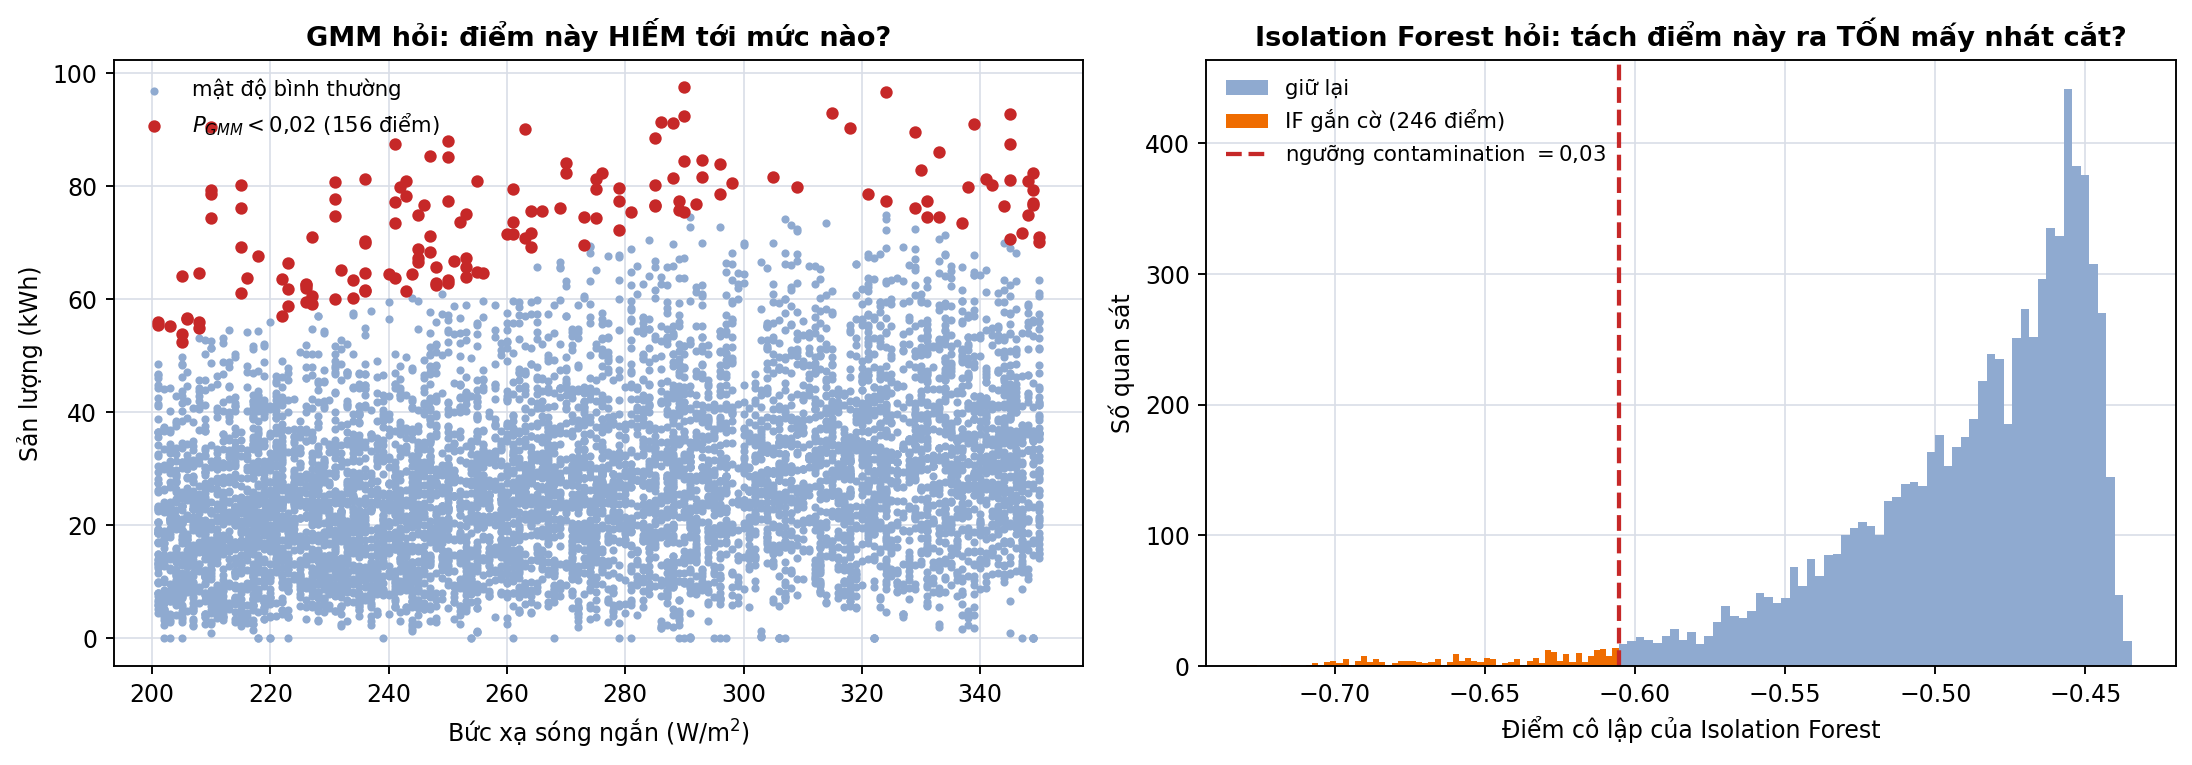
\includegraphics[width=\textwidth]{hai_nguyen_ly_tren_du_lieu_that.png}
    
    
    \caption{Phân bố mật độ GMM và điểm cô lập Isolation Forest trên dữ liệu trạm 27}
    \label{fig:hai_nguyen_ly}
\end{figure}

Hình~\ref{fig:hai_nguyen_ly} cho thấy hai thuật toán không thay thế được nhau. Nửa trái, GMM
gắn cờ $156$ điểm trên $8.176$ quan sát, tức $156 / 8.176 = 1{,}91\%$, toàn bộ nằm ở đuôi trên
của sản lượng và rải đều qua mọi mức bức xạ; đại lượng nó đo là mức hiếm của điểm trong phân
bố. Nửa phải, Isolation Forest gắn cờ $246$ điểm, tức $246 / 8.176 = 3{,}01\%$, theo một đại
lượng khác: số nhát cắt cần thiết để tách điểm đó khỏi phần còn lại.

Hai tập cờ không trùng nhau: phần giao chỉ còn $144$ điểm, tức GMM mất
$156 - 144 = 12$ điểm và Isolation Forest mất $246 - 144 = 102$ điểm khi bắt cả hai cùng đồng
ý. Có những điểm GMM cho là hiếm nhưng Isolation Forest thấy vẫn dễ giải thích, và ngược lại.
Pipeline lấy phép giao để chỉ giữ phần mà cả hai góc nhìn cùng đồng ý, sau đó hợp thêm với các
luật rào chắn vật lý.

Trên toàn bộ tệp đầu vào, cột \texttt{gmm\_if\_outlier\_flag} gắn cờ $\mathbf{7.431}$ dòng trên
tổng $\mathbf{2.731.946}$ dòng:

\begin{equation}
\frac{7.431}{2.731.946} = 0{,}002720 \;\longrightarrow\; \mathbf{0{,}27\%}
\end{equation}

Hai nhóm lý do chiếm phần lớn là đồng thuận GMM--IF ($6.102$ dòng) và bước nhảy phân phối cục bộ ($1.726$ dòng). Luật \texttt{PHYSICAL\_OVER\_CAPACITY} không gắn cờ dòng nào. Luật này so sản lượng của một
bước $15$ phút với mức mà công suất lắp đặt phát ra được trong $15$ phút, và chỉ gắn cờ khi
sản lượng vượt quá $1{,}20$ lần mức đó --- ngưỡng nới rộng để giữ lại các đỉnh do tăng cường
bức xạ ở mép mây. Cần nói rõ phạm vi: luật chỉ chạy trên những dòng có \texttt{capacity\_kw}
thật, nên $1.132.078$ dòng của $17$ trạm thiếu cột này nằm ngoài tầm xét của nó.

\subsubsection{Bốn phép đo thay cho precision và recall}

Phát hiện ngoại lai ở đây là bài toán học không giám sát, và bộ dữ liệu không đi
kèm nhãn sự cố do người vận hành xác nhận. Không có nhãn đối chiếu thì không tính được
precision, recall hay F-score, nói cách khác, không có cách nào chấm điểm một ngưỡng là
đúng hay sai. Vì vậy chất lượng của nhãn được đo bằng bốn đại lượng khác, mỗi đại lượng trả
lời một câu hỏi kiểm chứng được.

Một: chất lượng phân đoạn của cây quyết định. Bước phân đoạn được chấm bằng hệ
số xác định $R^2$, đo trên toàn bộ $42$ trạm: trung bình $0{,}758$, thấp nhất
$0{,}606$ và cao nhất $0{,}826$. Con số này không phải độ chính xác của bộ phát
hiện ngoại lai; nó chỉ đo mức các phân đoạn do cây tạo ra giữ được cấu trúc hình dạng phát
điện của từng trạm, tức mức phân đoạn đủ đồng nhất để chạy GMM bên trong. Hệ số $R^2$ tính
trên phần dư thấp hơn nhiều ($0{,}118$--$0{,}346$, trung bình $0{,}187$), đúng như kỳ vọng,
vì phần dư là phần biến động còn lại sau khi đã trừ ảnh hưởng của bức xạ nên chứa nhiều
nhiễu thời tiết và sai số cảm biến.

Hai: mức giảm cảnh báo khi bắt hai cơ chế cùng đồng ý. Phép giao giữa GMM và
Isolation Forest lọc bỏ phần lớn ứng viên của cả hai phía, xem Bảng~\ref{tab:song_sot_and}.

Bốn con số trong bảng dưới đây do script
\texttt{07\_local\_gmm\_if\_audit.py} trong \path{srcs/02_transform/02_generate_outliers/}
sinh ra. Script tách lại ba tệp đệm mà thuật toán cần từ bản kết xuất ML Mart, rồi gọi chính
\texttt{02\_gmm\_if.py} thay vì viết lại thuật toán.

\begin{table}[htbp]
\centering
\caption{Số lượng mẫu vượt qua điều kiện kết hợp GMM và Isolation Forest}
\label{tab:song_sot_and}
\small
\begin{tabular}{l r r r}
\toprule
\textbf{Cơ chế} & \textbf{Số ứng viên} & \textbf{Qua được phép giao} & \textbf{Tỷ lệ sống sót} \\
\midrule
GMM              & $34.431$ & $6.102$ & $17{,}72\%$ \\
Isolation Forest & $35.164$ & $6.102$ & $17{,}35\%$ \\
\bottomrule
\end{tabular}


\end{table}

Hai tỷ lệ sống sót trong bảng là thương của cột thứ ba trên cột thứ hai:

\begin{equation}
\text{GMM:}\ \frac{6.102}{34.431} = 0{,}1772 \quad\text{và}\quad
\text{Isolation Forest:}\ \frac{6.102}{35.164} = 0{,}1735
\end{equation}

Lớp đồng thuận vì vậy loại đi hơn bốn phần năm số cảnh báo của GMM và gần năm phần sáu số
cảnh báo của Isolation Forest. Tỷ lệ này đo mức giảm cảnh báo đơn lẻ; nó không tương
đương precision, vì phần bị loại chưa có nhãn xác nhận đúng hay sai.

Ba: khả năng tách hạng của điểm cô lập. Điểm cô lập trung bình của các dòng bị
gắn cờ cuối cùng là $\mathbf{0{,}5086}$, so với $\mathbf{0{,}2119}$ ở các dòng bình thường.
Khoảng cách giữa hai nhóm là $0{,}5086 - 0{,}2119 = \mathbf{0{,}2967}$, tức nhóm bị gắn cờ có
điểm cao gấp $0{,}5086 / 0{,}2119 = 2{,}40$ lần. Chênh lệch dương và ổn định cho thấy điểm số
có xếp hạng được hai nhóm, nhưng đây là bằng chứng về khả năng phân tách chứ không phải chứng
nhận độ chính xác.

Bốn: độ tái lập của năm luật rào chắn vật lý. Một quy tắc lọc dữ liệu chỉ đáng
tin nếu người khác dựng lại được đúng kết quả của nó. Nhóm viết lại toàn bộ năm luật trong
notebook \texttt{05d\_thuc\_nghiem\_rao\_chan\_vat\_ly}, đọc đúng ba tệp đệm mà tầng ETL đọc bảng
đệm sản lượng, bảng đệm thời tiết và bảng chiều trạm rồi đối chiếu từng dòng với cờ mà
tầng ETL đã ghi. Kết quả ở Bảng~\ref{tab:tai_lap_luat}.

\begin{table}[htbp]
\centering
\caption{Đối chiếu số lượng cờ dị thường với tầng ETL}
\label{tab:tai_lap_luat}
\small
\begin{tabular}{l r r r r}
\toprule
\textbf{Luật} & \textbf{Tầng ETL ghi} & \textbf{Dựng lại} & \textbf{Trùng} & \textbf{Độ khớp} \\
\midrule
\texttt{PHYSICAL\_OVER\_CAPACITY} ($> 1{,}20\times$) & $0$      & $0$      & $0$      & $100{,}0\%$ \\
\texttt{PHYSICAL\_HIGH\_ENERGY\_NO\_SUN}   & $33$     & $33$     & $33$     & $100{,}0\%$ \\
\texttt{PHYSICAL\_HIGH\_ENERGY\_LOW\_RAD}  & $131$    & $144$    & $125$    & $95{,}4\%$ \\
\texttt{PHYSICAL\_LOW\_ENERGY\_STRONG\_SUN}& $56$     & $56$     & $56$     & $100{,}0\%$ \\
\texttt{PHYSICAL\_DISTRIBUTION\_JUMP}      & $1.726$  & $1.726$  & $1.726$  & $100{,}0\%$ \\
\bottomrule
\end{tabular}


\end{table}

Bốn trên năm luật dựng lại bắt trọn $100\%$ số cờ tầng ETL đã ghi. Luật còn lại,
\texttt{PHYSICAL\_HIGH\_ENERGY\_LOW\_RAD}, đạt $95{,}4\%$: bản dựng lại bắt $144$ dòng so với
$131$ dòng tầng ETL ghi, trong đó $125$ dòng trùng nhau.

Cách dựng cận trên. Cận trên có dạng $Q_3 + m \cdot \texttt{safe\_IQR}$, trong đó
$IQR$ được tính riêng cho từng ô (trạm $\times$ mùa $\times$ dải bức xạ) chứ không
tính trên toàn chuỗi, để sản lượng của một điểm được so với đúng những điểm cùng hoàn cảnh
nắng.

Chuỗi sản lượng ban đầu có nhiều khoảng trống thời gian, nên sau khi chia theo ba chiều đó,
một số ô còn rất ít quan sát. Ô mỏng cho $IQR$ co gần về $0$; khi ấy cận
$Q_3 + 1{,}5 \cdot IQR$ nằm sát ngay $Q_3$ và sẽ gắn cờ hàng loạt điểm hoàn toàn bình
thường. Pipeline vì vậy đặt hai lớp bảo vệ:

\begin{itemize}
    \item \textbf{Nhánh dự phòng theo cỡ mẫu.} Ô nào có dưới $50$ quan sát thì bỏ chiều mùa,
    lấy thống kê của ô thô hơn (trạm $\times$ dải bức xạ) thay thế.
    \item \textbf{Sàn cho khoảng tứ phân vị.} Thay $IQR$ bằng
    $\texttt{safe\_IQR} = \max(IQR,\ 0{,}03 \cdot p_{95},\ 0{,}1)$, nên dù $IQR$ của ô có về
    $0$ thì cận vẫn còn một biên tối thiểu suy từ quy mô của chính trạm đó.
\end{itemize}

Hệ số nhân cũng nâng từ $1{,}5$ lên $4$ để cận nghiêm hơn, tránh gắn cờ những dao động do
mây che vốn hợp lệ.

Độ nhạy của ngưỡng. Cận $Q_3 + m \cdot \texttt{safe\_IQR}$ quyết định bao nhiêu
dòng bị loại khỏi tập huấn luyện, nên hệ số $m$ được quét qua sáu mức trên cùng dữ liệu,
từ mức Tukey chuẩn $1{,}5$ tới $6$. Kết quả ở Bảng~\ref{tab:quet_safe_iqr} và
Hình~\ref{fig:quet_safe_iqr}.

\begin{table}[htbp]
\centering
\caption{Ảnh hưởng của hệ số nhân \texttt{safe\_IQR} đến dữ liệu bị lọc}
\label{tab:quet_safe_iqr}
\small
\begin{tabular}{c r r r}
\toprule
\textbf{Hệ số $m$} & \textbf{Số dòng bị loại} & \textbf{Sản lượng bị loại (kWh)} & \textbf{Tỷ lệ trên tổng} \\
\midrule
$1{,}5$ & $693$ & $3.202$ & $0{,}0344\%$ \\
$2$     & $523$ & $2.610$ & $0{,}0280\%$ \\
$3$     & $245$ & $1.380$ & $0{,}0148\%$ \\
$\mathbf{4}$ \textbf{(đang dùng)} & $\mathbf{144}$ & $\mathbf{873}$ & $\mathbf{0{,}0094\%}$ \\
$5$     & $115$ & $649$   & $0{,}0070\%$ \\
$6$     & $69$  & $373$   & $0{,}0040\%$ \\
\bottomrule
\end{tabular}


\end{table}

\begin{figure}[htbp]
    \centering
    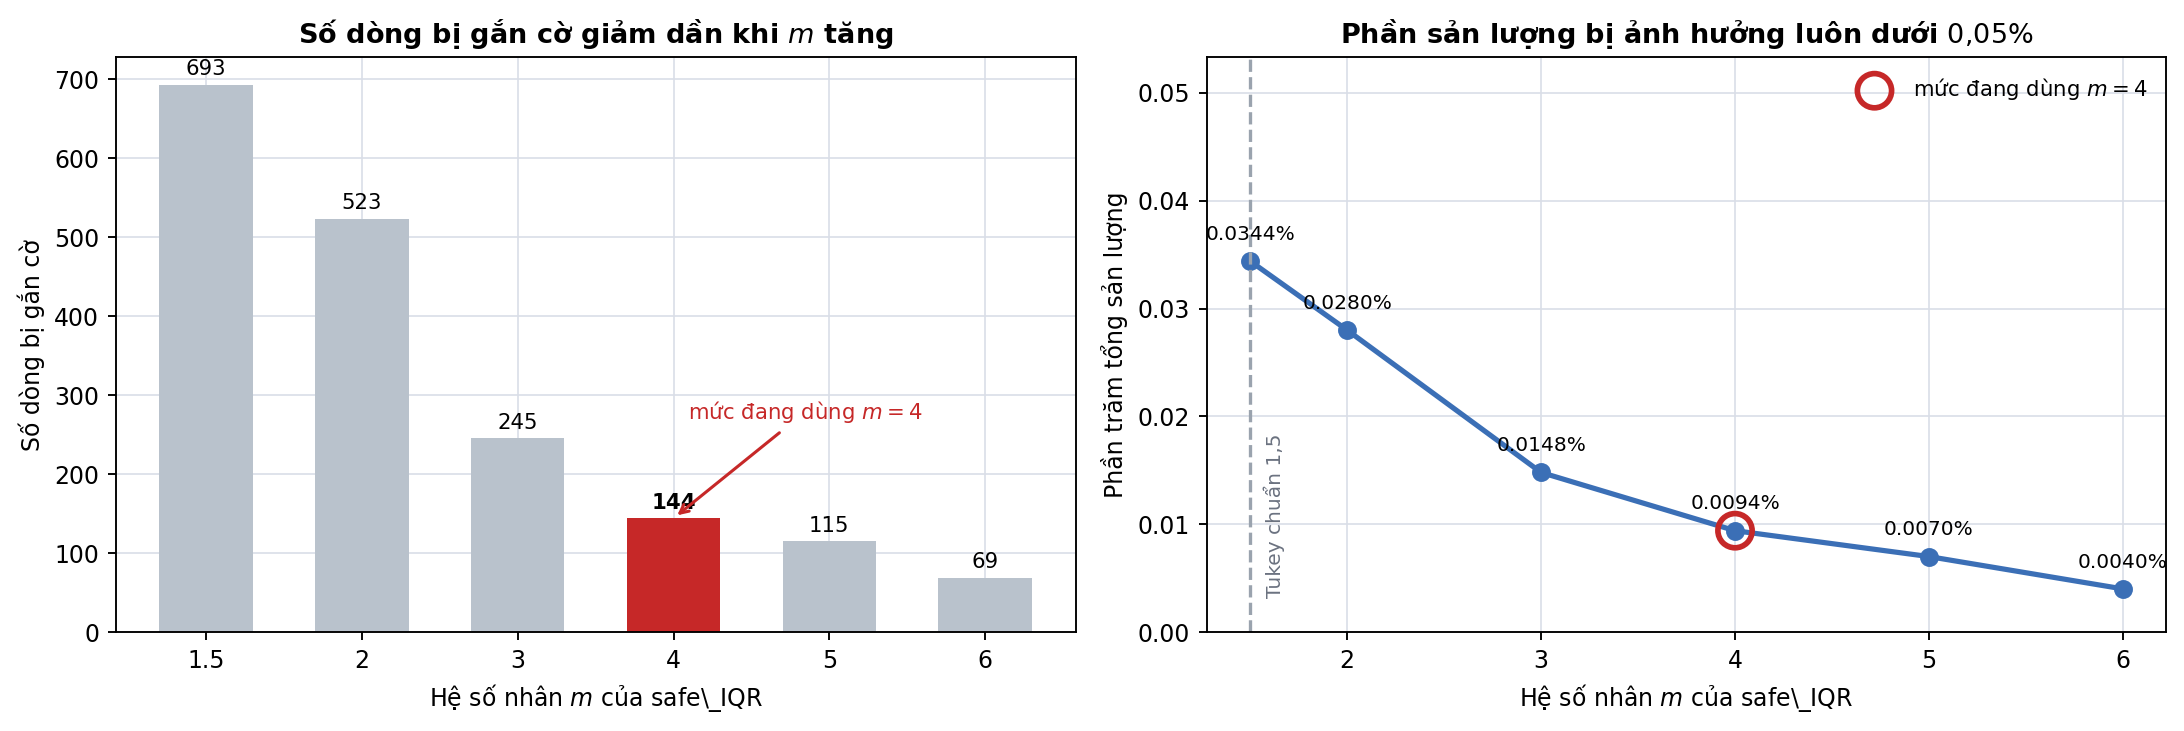
\includegraphics[width=\textwidth]{thuc_nghiem_quet_he_so_safe_iqr.png}
    
    
    \caption{Quét hệ số nhân $m$ của \texttt{safe\_IQR} qua sáu mức}
    \label{fig:quet_safe_iqr}
\end{figure}

Nhìn Hình~\ref{fig:quet_safe_iqr} thấy hai điều. Số dòng bị gắn cờ giảm đều khi $m$ tăng,
đường giảm liên tục và không có bậc nhảy nào cho thấy một mức $m$ đặc biệt tự tách
ra khỏi phần còn lại. Phần sản lượng bị ảnh hưởng nằm gọn dưới mốc $0{,}05\%$ trên toàn dải,
cao nhất $0{,}0344\%$ tại $m = 1{,}5$ và thấp nhất $0{,}0040\%$ tại $m = 6$, chênh nhau
vỏn vẹn $0{,}03$ điểm phần trăm.

Hai quan sát trên dẫn tới một kết luận: dù chọn hệ số nào trong khoảng
$1{,}5$--$6$, lượng dữ liệu bị loại đều không vượt quá một phần nghìn của bộ dữ liệu, nên
lựa chọn hệ số ít ảnh hưởng tới kết quả mô hình. Mức $4$ đang dùng là một
quyết định nằm trong vùng an toàn, không phải một mức tối ưu đã được chứng minh.

% Mục này gồm sơ đồ 8 bước và bảng ánh xạ, hai float lớn không nhét vừa cuối trang
% trước. Cho mục bắt đầu trang mới để hình và bảng nằm đúng trong mục của nó, thay vì
% bị đẩy sang sau khi mục 1.5 đã mở.
\FloatBarrier
\subsection{Sơ đồ toàn cảnh}
\label{subsec:so_do_toan_canh}

Trước khi đi vào quy trình cụ thể của đề tài, Hình~\ref{fig:ml_lifecycle} nhắc lại vòng đời
học máy ở dạng chung nhất. Vòng ngoài màu xanh là phần gắn với bài toán: xuất phát từ yêu cầu
nghiệp vụ, xác định bài toán, rồi ở cuối là triển khai, giám sát và phân tích thông tin thu
được. Vòng trong màu cam là phần gắn với dữ liệu và mô hình, chạy từ thu thập, xử lý, sinh đặc
trưng, huấn luyện đến đánh giá. Điểm cần chú ý là cả hai vòng đều khép kín: kết quả giám sát
quay ngược về yêu cầu nghiệp vụ, và kết quả đánh giá quay ngược về khâu dữ liệu.

\begin{figure}[!htbp]
    \centering
    \resizebox{0.68\textwidth}{!}{%
    \begin{tikzpicture}[
      hopxanh/.style={
        draw=tblNavy, line width=1.1pt, fill=blue!10, rounded corners=9pt,
        align=center, inner sep=4pt, text width=4.15cm, minimum height=2.3cm,
        font=\large\bfseries, text=tblNavy
      },
      hopcam/.style={
        draw=tblOrange, line width=1.1pt, fill=orange!10, rounded corners=9pt,
        align=center, inner sep=4pt, text width=3.75cm, minimum height=2.15cm,
        font=\large\bfseries, text=tblOrange!90!black
      }
    ]
    \def\Rx{7.05}   \def\Cy{3.30}
    \def\Rc{4.50}

    \fill[orange!15] (0,0) circle (\Rc);
    \draw[tblOrange, line width=7pt] (0,0) circle (\Rc);

    \draw[tblNavy, line width=6pt]
      ([shift={(0,\Cy)}]-27:\Rx) arc[start angle=-27, end angle=207, radius=\Rx];

    % Bon hop tren cung xanh
    \node[hopxanh] at ($(0,\Cy)+(131.3:\Rx)$) {Giám sát\\Phân tích thông tin};
    \node[hopxanh] at ($(0,\Cy)+( 50.6:\Rx)$) {Yêu cầu\\nghiệp vụ};
    \node[hopxanh] at ($(0,\Cy)+( 10.3:\Rx)$) {Xác định\\bài toán};
    \node[hopxanh] at ($(0,\Cy)+(170.3:\Rx)$) {Triển khai mô hình};

    % Nam hop tren vong cam
    \node[hopcam] at ( 89.3:\Rc) {Thu thập\\dữ liệu};
    \node[hopcam] at ( 10.5:\Rc) {Xử lý\\dữ liệu};
    \node[hopcam] at (-43.2:\Rc) {Sinh\\đặc trưng};
    \node[hopcam] at (227.8:\Rc) {Huấn luyện\\mô hình};
    \node[hopcam] at (170.3:\Rc) {Đánh giá\\mô hình};
    \end{tikzpicture}%
    }
    
    
    \caption{Vòng đời phát triển và vận hành mô hình học máy (MLOps)~\cite{aivietnam2025dvc}}
    \label{fig:ml_lifecycle}
\end{figure}

Quy trình của đề tài là một lần hiện thực hoá vòng đời đó.
Hình~\ref{fig:pipeline_mlops} mô tả chín bước của quy trình. Bốn bước đầu lấy, làm sạch,
chia và khảo sát dữ liệu; bước $5$ sinh rồi chọn đặc trưng; bốn bước cuối huấn luyện,
đánh giá, đưa mô hình vào sử dụng và quản lý phiên bản dữ liệu cùng mô hình.

\begin{figure}[!htbp]
    \centering
    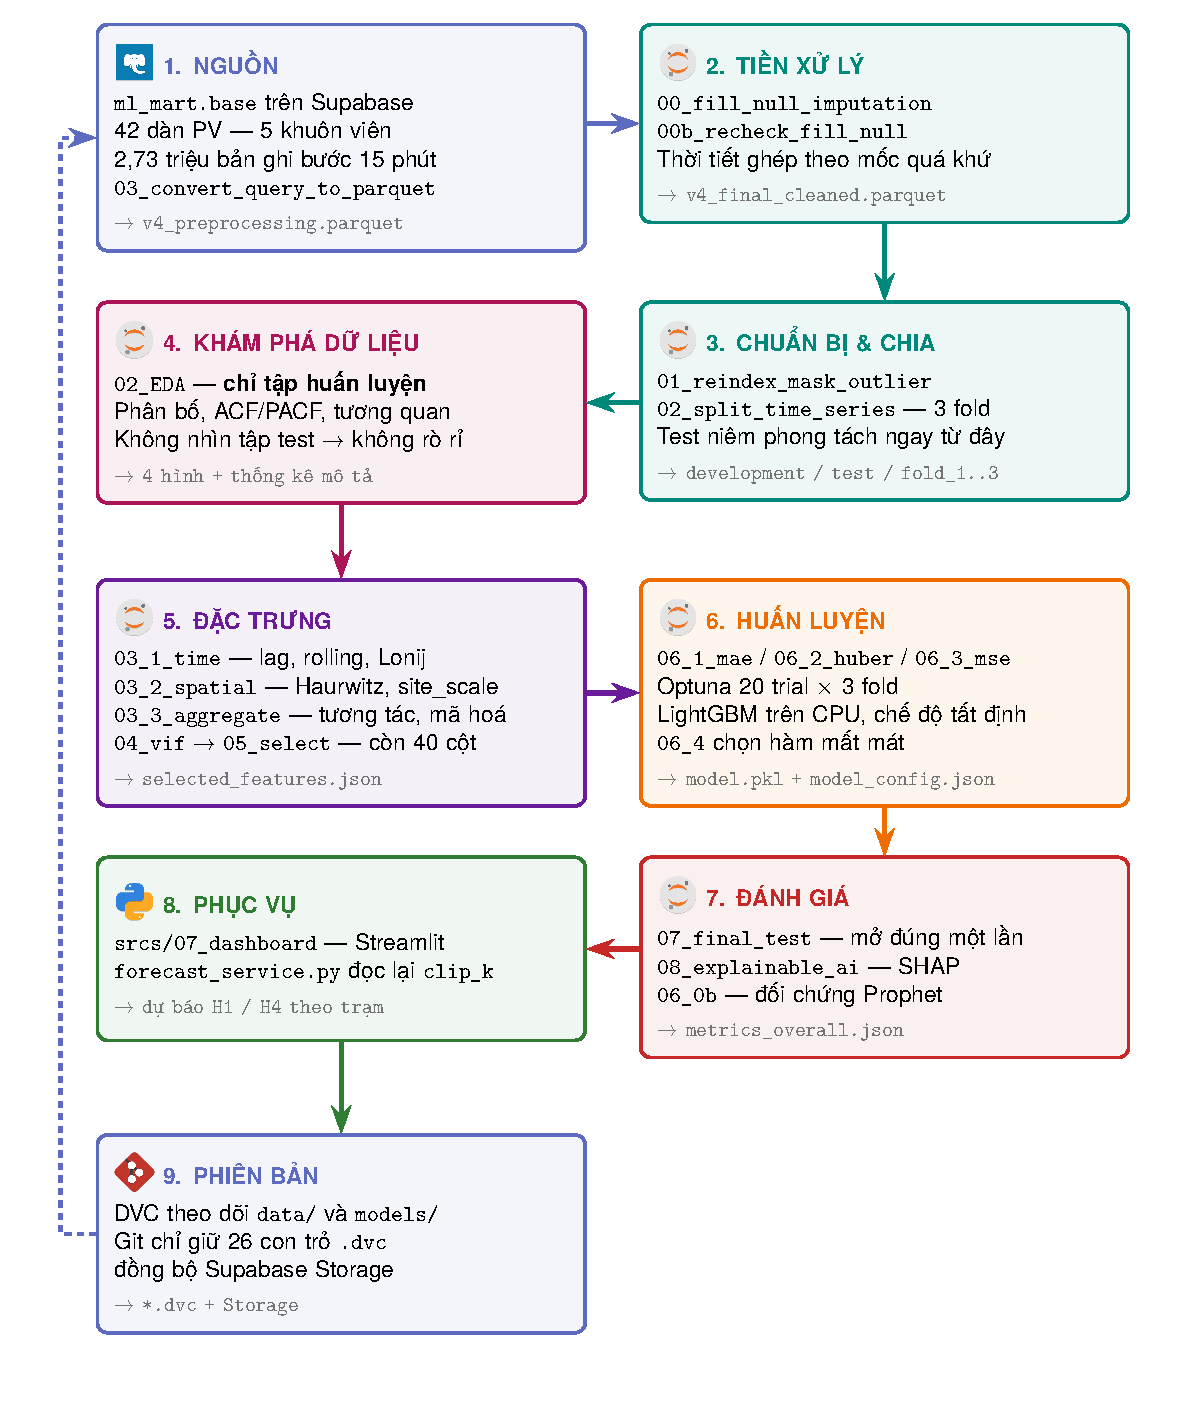
\includegraphics[width=0.96\textwidth]{pipeline_sodo_mlops.pdf}
    
    
    \caption{Quy trình 9 bước phát triển và đánh giá mô hình học máy}
    \label{fig:pipeline_mlops}
\end{figure}

Mỗi bước tương ứng với một notebook trong thư mục
\path{notebooks/forcasting_v5_energy/}. Toàn bộ số liệu và hình ảnh trong các phần
sau đều trích từ những tệp kết quả liệt kê ở Bảng~\ref{tab:notebook_pipeline}.

\begin{table}[htbp]
\centering
\caption{Ánh xạ các bước trong quy trình với notebook thực hiện}
\label{tab:notebook_pipeline}
\footnotesize
% Giãn dòng toàn cục 1,35 làm bảng 13 dòng cao thêm hơn một phần tư và không nhét
% vừa phần còn lại của trang. Đưa về 1,0 trong phạm vi bảng này.
\renewcommand{\baselinestretch}{1.0}\selectfont
% Cot 3 phai du 5,4cm: ten tep dai nhat la prophet_test_summary.json, 25 ky tu chu
% don cach chiem 5,27cm. Bu lai bang cach thu cot 1 - cot do la chu tieng Viet nen
% ngat dong duoc, khong tran. Tong ba cot giu nguyen 13,4cm.
\begin{tabular}{@{}p{3.4cm} p{4.6cm} p{5.4cm}@{}}
\toprule
\textbf{Bước} & \textbf{Notebook} & \textbf{Kết quả ghi ra} \\
\midrule
Chuẩn bị lưới thời gian & \texttt{01\_reindex\_mask\_outlier} & lưới $15$ phút liên tục \\
Chia dữ liệu & \texttt{02\_split\_time\_series} & $3$ fold và tập test niêm phong \\
Khám phá dữ liệu & \texttt{02\_EDA} & thống kê mô tả, ACF/PACF, tương quan \\
Đặc trưng thời gian & \texttt{03\_1\_features\_time} & lag, rolling, chu kỳ lịch \\
Đặc trưng không gian & \texttt{03\_2\_features\_spatial} & solar geometry, \texttt{site\_scale} \\
Đặc trưng tương tác & \texttt{03\_3\_features\_aggregate} & tương tác, mã hoá phân loại \\
Chẩn đoán đa cộng tuyến & \texttt{04\_vif\_diagnostics} & bảng hệ số VIF \\
Chọn đặc trưng & \texttt{05\_select\_features} & \texttt{selected\_features.json} \\
Huấn luyện & \texttt{06\_1}, \texttt{06\_2}, \texttt{06\_3} & \texttt{model.pkl}, \texttt{model\_config.json} \\
Chọn hàm mất mát & \texttt{06\_4\_validate\_model} & bảng đối chiếu ba hàm \\
Đánh giá cuối & \texttt{07\_final\_test} & \texttt{metrics\_overall.json} \\
Giải thích mô hình & \texttt{08\_explainable\_ai} & biểu đồ SHAP \\
Mô hình đối chứng & \texttt{07b\_baseline\_prophet} & \texttt{prophet\_test\_summary.json} \\
\bottomrule
\end{tabular}


\end{table}

\FloatBarrier
\subsection{Năm rào chắn chống rò rỉ dữ liệu}
\label{subsec:nam_rao_chan}

Rò rỉ dữ liệu là rủi ro lớn nhất của một bài toán dự báo chuỗi thời gian: chỉ cần một
đặc trưng vô tình mang thông tin của tương lai, mọi chỉ số đánh giá đều trở nên vô
nghĩa. Quy trình đặt năm rào chắn, mỗi rào chắn gắn với một bước cụ thể:

\begin{enumerate}
    \item \textbf{Nhân quả trong ghép thời tiết} (bước $2$). Mỗi bản ghi tại thời điểm
    $T$ chỉ được ghép với khối khí tượng của giờ đã kết thúc trước $T$. Điều kiện này
    được kiểm tra trên toàn bộ $2{,}73$ triệu bản ghi.

    \item \textbf{Không chồng lấn khi chia dữ liệu} (bước $3$). Dữ liệu được cắt theo
    trục thời gian, không xáo trộn ngẫu nhiên. Tập test được tách ra trước mọi bước
    khác, và trong quy trình này chỉ được đọc ở bước $7$.

    \item \textbf{Thống kê tính riêng theo từng fold} (bước $5$). Các đại lượng tổng
    hợp như \texttt{site\_scale} hay \texttt{cs\_factor} được ước lượng riêng trong
    phần huấn luyện của từng fold, không nhìn sang phần kiểm định.

    \item \textbf{Ngưỡng suy từ dữ liệu huấn luyện} (bước $6$). Cận cắt của mục tiêu
    chuẩn hoá được tính từ phân vị của dữ liệu huấn luyện, rồi ghi vào tệp cấu hình để
    các bước sau đọc lại đúng giá trị đó thay vì tính lại trên tập khác.

    \item \textbf{Tái lập được} (bước $6$). LightGBM chạy ở chế độ tất định trên CPU với
    \texttt{deterministic} $=$ true, \texttt{force\_col\_wise} $=$ true và
    \texttt{random\_state} $=42$; toàn bộ siêu tham số của sáu cấu hình được ghi ra
    \texttt{model\_config.json} để đối chiếu.
\end{enumerate}

Bốn rào chắn đầu được kiểm chứng bằng số liệu ở các phần tương ứng phía sau. Rào chắn
thứ năm được bảo đảm bằng cấu hình tất định, trình bày ở Mục~\ref{subsec:cau_hinh_tat_dinh}.

\FloatBarrier
\section{Chuẩn bị dữ liệu và chia tập}

Mục này đi từ tệp đã làm sạch tới các tập sẵn sàng huấn luyện, qua sáu bước: hiện trạng dữ
liệu, dựng lại lưới thời gian, khám phá dữ liệu, cắt tập test niêm phong, chia ba fold kiểm
định, và đo nhãn chồng lấn ở ranh giới fold.

\FloatBarrier
\subsection{Hiện trạng bộ dữ liệu}
\label{subsec:hien_trang_du_lieu}

Sau khi dựng lại lưới, bộ dữ liệu có $2.784.438$ dòng của $42$ vị trí lắp đặt, trải từ
$01/01/2020$ đến $23/04/2022$ ở bước $15$ phút, trong đó $52.492$ dòng ($1{,}89\%$) là mốc
được chèn thêm cho lưới khỏi đứt quãng.

Chỉ $1.195.645$ dòng ($42{,}94\%$) là số đo thật. Phần còn lại do tầng ETL xử lý: $1.536.301$
dòng điền khuyết ($55{,}17\%$); cách điền từng nhóm thuộc phạm vi tầng ETL. Ngoài ra, tầng ETL gắn cờ ngoại lai cho $7.431$ dòng ($0{,}27\%$), gồm $6.102$ dòng do hai cơ chế thống kê GMM--IF cùng đồng ý ($5.556$ dòng thuần $GMM \wedge IF$ và $546$ dòng kết hợp luật vật lý) cùng $1.329$ dòng trúng các luật rào chắn vật lý độc lập (chủ yếu là bước nhảy phân phối cục bộ $1.211$ dòng và bất thường bức xạ $118$ dòng); Mục~\ref{subsec:ngoai_lai_etl} và Bảng~\ref{tab:tai_lap_luat} kiểm chứng lại các cờ này.

Bốn điểm trên định hình các bước còn lại. Lưới đứt quãng phải dựng lại trước tiên, vì đặc
trưng trễ và cửa sổ trượt đếm theo số bước chứ không theo mốc đồng hồ nên một lỗ hổng làm chúng
tính sai mà không báo lỗi. Tỷ lệ đo thật thấp không sửa được bằng kỹ thuật nên xử lý bằng chính
sách: dòng không phải số đo thật, kể cả dòng mang cờ ngoại lai, nhận trọng số $0$ khi huấn luyện
và bị loại khỏi phạm vi chấm điểm, nhưng vẫn giữ trong lưới để không đứt lịch sử.

Hai điểm nữa cũng chi phối các bước sau: dữ liệu khí tượng chỉ có độ hạt một giờ nên mỗi giá trị
bức xạ lặp bốn lần và cần một bước hạ độ hạt riêng; và $42$ vị trí lắp đặt chênh nhau nhiều về
quy mô nên mục tiêu phải chuẩn hoá theo từng trạm, nếu không phần lớn sức mô tả của mô hình dành cho việc phân biệt trạm
lớn với trạm nhỏ thay vì học quan hệ giữa thời tiết và sản lượng.

\FloatBarrier
\subsection{Dựng lại lưới thời gian liên tục}

Dữ liệu sản lượng thu từ công tơ không phải lúc nào cũng đủ mốc: mất điện, mất kết nối
hoặc lỗi ghi đều để lại lỗ hổng trên trục thời gian. Nếu đưa thẳng dữ liệu khuyết mốc
vào bước sinh đặc trưng, các biến trễ và biến cửa sổ trượt sẽ tính sai, \texttt{lag\_4}
lẽ ra phải lùi đúng $60$ phút thì lại lùi $75$ hay $90$ phút, tuỳ vào chỗ bị khuyết.

Notebook \texttt{01\_reindex\_mask\_outlier} dựng lại lưới $15$ phút liên tục cho từng trạm
bằng \texttt{pd.date\_range}, rồi đánh dấu những dòng vừa được chèn thêm. Thứ tự hai
việc này là điều kiện bắt buộc: dựng lưới trước, lọc sau. Nếu lọc bỏ dòng ban
đêm hay dòng ngoại lai trước khi dựng lưới, khoảng cách thời gian giữa các dòng còn lại
sẽ không đều, và mọi đặc trưng trễ sau đó đều lệch.

Các dòng bị gắn cờ ngoại lai ở tầng ETL không bị xoá khỏi lưới. Chúng được giữ nguyên
vị trí để lịch sử không bị đứt quãng, nhưng mang nhãn loại trừ nên không đóng góp vào
hàm mất mát khi huấn luyện, cũng không tham gia vào các chỉ số được báo cáo.

Ba ràng buộc thiết kế. Bước dựng lưới tuân thủ ba ràng buộc, cùng hướng tới một
mục tiêu: không để thông tin của tương lai, hoặc thông tin không có thật, lọt vào lưới dữ liệu.

\begin{enumerate}
    \item \textbf{Thời tiết chỉ được lấp theo chiều tiến.} Chỉ dùng \texttt{ffill()} theo
    từng trạm, tức sử dụng giá trị đã quan sát trong quá khứ sang hiện tại. Quy trình nghiêm cấm
    dùng \texttt{bfill()}, vì kéo ngược là lấy giá trị của mốc sau đắp cho mốc trước --- đúng
    định nghĩa của rò rỉ dữ liệu.
    \item \textbf{Siêu dữ liệu tĩnh thiếu thì giữ nguyên khuyết.} Các cột như
    \texttt{capacity\_kw}, \texttt{number\_of\_panels}, vĩ độ và kinh độ nếu thiếu thì để nguyên
    khuyết, không lấp và không bịa giá trị.
    \item \textbf{Điền mục tiêu theo bậc thang nhân quả.} Slot mới chèn được điền theo đúng
    thứ tự: \texttt{night\_zero} $\rightarrow$ \texttt{causal\_day\_persistence} (cùng giờ hôm qua)
    $\rightarrow$ \texttt{causal\_week\_persistence} (cùng giờ tuần trước) $\rightarrow$
    \texttt{causal\_profile\_median} $\rightarrow$ \texttt{fallback\_zero}. Mọi bậc đều chỉ nhìn về
    quá khứ. Riêng khoảng trống từ $24$ giờ trở lên được xếp vào \texttt{machine\_failure\_zero}
    và đánh dấu loại khỏi huấn luyện.
\end{enumerate}

Kết quả thực thi. Khối dưới đây trích nguyên văn kết quả kết xuất của notebook
\texttt{01\_reindex\_mask\_outlier}:

% Khoi ket xuat notebook. Khong boc trong minipage nua: minipage la mot hop lien
% khoi, khong the ngat trang, nen khoi dai bi day nguyen sang trang sau va de lai
% khoang trong lon. De verbatim o muc doan van thi no tu ngat duoc.
\begingroup
\par\penalty-150\vspace{8pt}
\small\renewcommand{\baselinestretch}{1.0}\selectfont
\begin{verbatim}
Đã reindex lưới 15 phút cho 42 site.
Tổng số dòng sau reindex: 2784438
- Dòng gốc: 2731946
- Dòng inserted: 52492

Forward-fill thời tiết (causal only, per-site):
- Số cột thời tiết: 15
- NaN trước: 812250
- NaN sau: 1890
- Đã lấp: 810360 giá trị

Đã điền target cho 52492 slot inserted.

--- PHÂN BỐ ENERGY_SOURCE SAU CASCADE ---
energy_source
etl_imputed                1536301
measured                   1195645
machine_failure_zero         42055
night_zero                    6287
causal_day_persistence        2668
fallback_zero                  984
causal_profile_median          283
causal_week_persistence        215

--- GATE CHECK ---
- Target null: 0
- Energy_source rỗng: 0
PASS - Không còn target null hoặc energy_source rỗng.
\end{verbatim}
\par\vspace{8pt}
\endgroup

Phân tích kết quả. Sáu nhãn thuộc bậc thang điền \texttt{machine\_failure\_zero},
\texttt{night\_zero}, \texttt{causal\_day\_persistence}, \texttt{fallback\_zero},
\texttt{causal\_profile\_median} và \texttt{causal\_week\_persistence} cộng lại bằng đúng
$52.492$, tức đúng số dòng đã chèn. Không dòng nào rơi ra ngoài bậc thang, cũng không dòng
nào bị đếm hai lần. Cổng kiểm ở cuối xác nhận không còn mục tiêu khuyết và không còn
\texttt{energy\_source} rỗng.

Hạn chế của bước dựng lưới. Trong $52.492$ dòng được chèn thì $42.055$ dòng rơi vào
nhãn \texttt{machine\_failure\_zero}, tức các khoảng trống từ $24$ giờ trở lên, được gán $0$ và
loại khỏi huấn luyện:

\begin{equation}
\frac{42.055}{52.492} = 0{,}8012 \;\longrightarrow\; \mathbf{80{,}1\%}
\end{equation}

Bốn phần năm phần chèn thêm vì vậy không mang thông tin mới; chúng chỉ giữ chỗ để
lưới thời gian không bị đứt. Phần còn lại được điền bằng các bậc suy từ lịch sử thật, gồm
$6.287 + 2.668 + 984 + 283 + 215 = 10.437$ dòng, trong đó $6.287$ dòng là \texttt{night\_zero} ---
các mốc ban đêm vốn phải bằng $0$. Số dòng thực sự được suy từ lịch sử phát điện là
$10.437 - 6.287 = 4.150$ dòng.

Một hạn chế nữa: sau khi lấp theo chiều tiến vẫn còn $1.890$ ô thời tiết khuyết. Đó là các mốc
nằm ở đầu chuỗi của từng trạm, nơi chưa có quan sát quá khứ nào để kéo sang. Chỉ có thể lấp
những ô này bằng phép lấp ngược chiều, tức lấy giá trị của mốc sau đắp cho mốc trước, mà phép đó
đưa thông tin tương lai vào dữ liệu huấn luyện. Quy trình vì vậy giữ nguyên trạng thái khuyết
ở các mốc đó, đổi lấy việc bảo toàn ràng buộc nhân quả. Theo khối kết xuất ở trên, phép lấp
theo chiều tiến xử lý được $810.360$ trên $812.250$ ô khuyết ban đầu, tức
$810.360 / 812.250 = 99{,}77\%$; phần còn lại là $1.890$ ô. LightGBM nhận trực tiếp giá trị
khuyết nên phần này không cần điền.

Cách xử lý này phù hợp với kết quả của Kim, Ko và Kim~\cite{kim2019missing}. Nhóm tác
giả đánh giá tác động của dữ liệu khuyết tới bài toán dự báo sản lượng quang điện và
chỉ ra rằng cách xử lý phần khuyết ảnh hưởng trực tiếp tới sai số của mô hình dự báo,
chứ không phải là một bước tiền xử lý trung tính:

\begin{quote}\small
\textit{``Such missing values deteriorate the PV power generation prediction performance, and they need to be eliminated by filling in other values.''}
\end{quote}


Từ đó, dự án tách bạch hai việc: dựng lại mốc thời gian để cấu trúc chuỗi
không bị đứt, và đánh dấu nguồn gốc từng dòng để phần dữ liệu không đáng tin
không lọt vào chỉ số báo cáo. Phạm vi của bài báo và của dự án khác nhau ở một điểm: bài báo khảo
sát bốn phương pháp điền khuyết cho dữ liệu khí tượng và kết luận phương pháp
$k$ láng giềng gần nhất cho kết quả tốt nhất, trong khi dự án chỉ mượn kết luận tổng
quát rằng phần khuyết phải được xử lý có chủ đích.

\FloatBarrier
\subsection{Phân tích khám phá dữ liệu và các quyết định sinh đặc trưng}
\label{subsec:kham_pha_du_lieu}

Trước khi sinh đặc trưng, dữ liệu được khảo sát ở notebook \texttt{02\_EDA}. Phạm vi khảo sát là
chỉ tập huấn luyện, sau khi loại hai trạm $19$ và $24$: còn $1.480.000$ dòng của
$40$ trạm. Đây là điều kiện bắt buộc các quyết định sinh đặc trưng ở Phần~$3$ đều rút ra
từ bước này, nên nếu khảo sát cả tập test thì tập test đã tham gia vào thiết kế mô hình,
trái với nguyên tắc niêm phong nêu ở Mục~\ref{subsec:nam_rao_chan}.

Ba phạm vi con được tách riêng để mọi con số phía sau đều nói rõ nó thuộc phạm vi nào:

% Khoi ket xuat notebook. Khong boc trong minipage nua: minipage la mot hop lien
% khoi, khong the ngat trang, nen khoi dai bi day nguyen sang trang sau va de lai
% khoang trong lon. De verbatim o muc doan van thi no tu ngat duoc.
\begingroup
\par\penalty-150\vspace{8pt}
\small\renewcommand{\baselinestretch}{1.0}\selectfont
\begin{verbatim}
Doc vao          : 1,550,856 dong x 12 cot | 42 tram
Sau khi bo tram [19, 24]: 1,480,000 dong | 40 tram

   toan bo               1,480,000 dong  (100.00%)
   ban ngay                742,116 dong  (50.14%)
   do that ban ngay        606,112 dong  (40.95%)
\end{verbatim}
\par\vspace{8pt}
\endgroup
\subsubsection{Phân bố đơn biến của sản lượng}

\begin{table}[htbp]
\centering
\caption{Thống kê mô tả sản lượng theo ba phạm vi}
\label{tab:eda_mo_ta}
\small
\begin{tabular}{l r r r r r}
\toprule
\textbf{Phạm vi} & \textbf{Số dòng} & \textbf{Trung vị} & \textbf{Độ lệch} & \textbf{Độ nhọn} & \textbf{\% bằng $0$} \\
\midrule
Toàn bộ          & $1.480.000$ & $0{,}0000$ & $6{,}0575$ & $47{,}3227$ & $52{,}47$ \\
Ban ngày         & $742.116$   & $2{,}7383$ & $4{,}5130$ & $25{,}3731$ & $6{,}04$ \\
Đo thật ban ngày & $606.112$   & $3{,}2188$ & $4{,}4313$ & $24{,}5310$ & $0{,}00$ \\
\bottomrule
\end{tabular}


\end{table}

Phân bố lệch phải rất mạnh và nhọn: trên toàn bộ tập huấn luyện, độ lệch đạt $6{,}06$ và độ
nhọn đạt $47{,}32$, trong khi phân phối chuẩn có cả hai bằng $0$. Nguyên nhân trực tiếp là
$52{,}47\%$ số quan sát bằng $0$, ban đêm và các khung giờ rìa ngày. Trung vị của
toàn bộ tập cũng bằng $0$, tức quá nửa dữ liệu không mang thông tin phát điện.

Hình~\ref{fig:eda_phan_bo} trình bày ba cách nhìn cùng một phân bố.
Lọc về ban ngày kéo độ lệch xuống $4{,}51$ và tỷ lệ giá trị $0$ xuống $6{,}04\%$; lọc thêm
điều kiện đo thật thì không còn giá trị $0$ nào. Ba dòng của Bảng~\ref{tab:eda_mo_ta} vì vậy
là căn cứ trực tiếp cho hai quyết định: chỉ tính chỉ số báo cáo trên phạm vi đo thật
ban ngày, và chuẩn hoá mục tiêu để kéo phân bố về dạng đều hơn.

\begin{figure}[htbp]
    \centering
    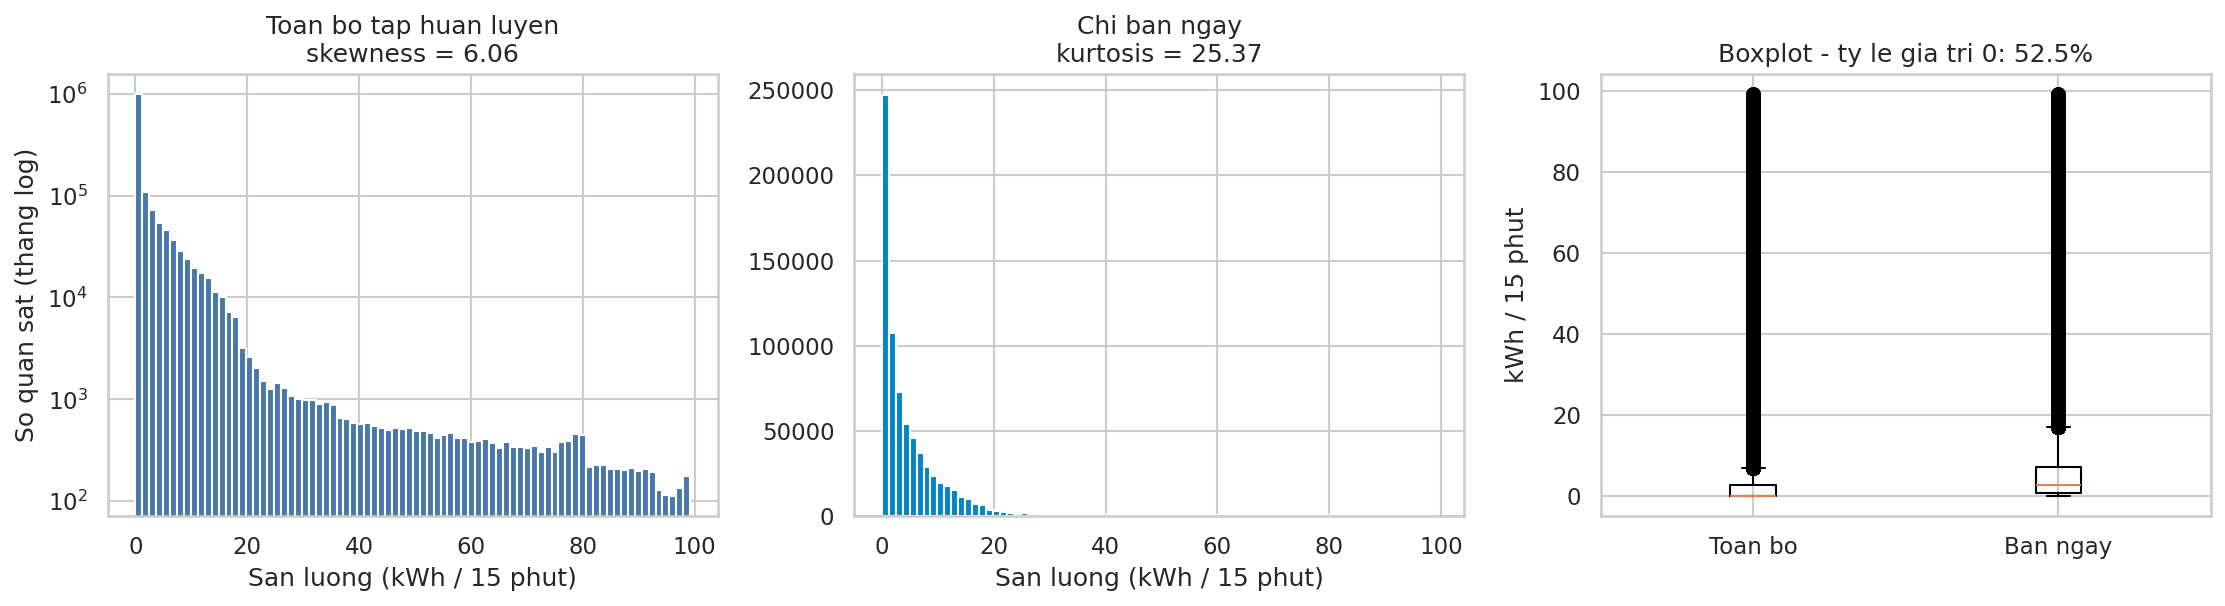
\includegraphics[width=\textwidth]{eda_phan_bo_don_bien.png}
    
    
    \caption{Phân phối sản lượng trên tập huấn luyện theo các phạm vi}
    \label{fig:eda_phan_bo}
\end{figure}

\subsubsection{Mẫu hình phát điện và tác động của mây}

Hai dạng ngày cho hai dạng chuỗi khác hẳn nhau. Ngày trời quang cho đường cong trơn dạng
parabol; ngày nhiều mây cho chuỗi gãy khúc liên tục. Notebook chọn hai ngày tương phản trên
trạm phát mạnh nhất, và chỉ xét những ngày có ít nhất $40$ mốc đo thật ban ngày cùng đủ $96$
mốc trong ngày, để hình không rơi vào ngày do tầng ETL điền khuyết:

% Khoi ket xuat notebook. Khong boc trong minipage nua: minipage la mot hop lien
% khoi, khong the ngat trang, nen khoi dai bi day nguyen sang trang sau va de lai
% khoang trong lon. De verbatim o muc doan van thi no tu ngat duoc.
\begingroup
\par\penalty-150\vspace{8pt}
\small\renewcommand{\baselinestretch}{1.0}\selectfont
\begin{verbatim}
Tram 27 | 283 ngay dat dieu kien | 71 ngay nhieu nang
   Ngay troi quang: 2020-10-02 | do gap 0.0031
   Ngay nhieu may : 2020-12-23 | do gap 0.0926
\end{verbatim}
\par\vspace{8pt}
\endgroup
Hai ngày này không được chọn bằng mắt mà bằng một đại lượng đo trực tiếp trên chuỗi sản
lượng, gọi là độ gấp: trung bình trị tuyệt đối của sai phân bậc hai trong ngày, chia
cho đỉnh của chính ngày đó. Sai phân bậc hai đo mức đổi hướng giữa ba mốc liên tiếp, nên
đường càng trơn thì độ gấp càng nhỏ; phép chia cho đỉnh khiến chỉ số không phụ thuộc quy mô
trạm. Phép chọn chỉ xét trong nhóm $71$ ngày nhiều nắng, nhóm có tổng sản lượng
thuộc phần tư trên, rồi lấy ngày độ gấp nhỏ nhất làm ngày trời quang và ngày độ gấp lớn
nhất làm ngày nhiều mây. Ràng buộc nhóm là cần thiết: một ngày âm u kéo dài cũng cho đường
phẳng lì và độ gấp rất nhỏ, nếu không lọc trước thì nó sẽ bị chọn nhầm thành ngày trời quang.

Hình~\ref{fig:eda_mau_hinh} đặt hai ngày cạnh nhau trên cùng thang trục tung. Ngày
$02/10/2020$ cho một đường cong trơn, lên đều rồi hạ gần đối xứng. Ngày $23/12/2020$ đạt
đỉnh tương đương nhưng chỉ giữ được trong ít bước, phần còn lại là chuỗi răng cưa. Độ gấp của
hai ngày chênh nhau gần $30$ lần: $0{,}0926 / 0{,}0031 = 29{,}9$.

Cả hai đều thuộc nhóm ngày nhiều nắng, tức lượng bức xạ khả dụng trong ngày tương đương, nhưng
cho hai chuỗi khác hẳn. Phần chênh lệch đó là do mây, và mô hình không thể suy ra nó từ lịch
hay từ vị trí Mặt Trời. Đây là căn cứ sinh hai đặc trưng \texttt{chi\_so\_troi\_quang} và
\texttt{rad\_x\_sinelev}: chúng cấp cho mô hình tín hiệu về mức che phủ ngay tại bước hiện
tại, thay vì bắt mô hình suy ra gián tiếp từ các mốc trễ.

\begin{figure}[htbp]
    \centering
    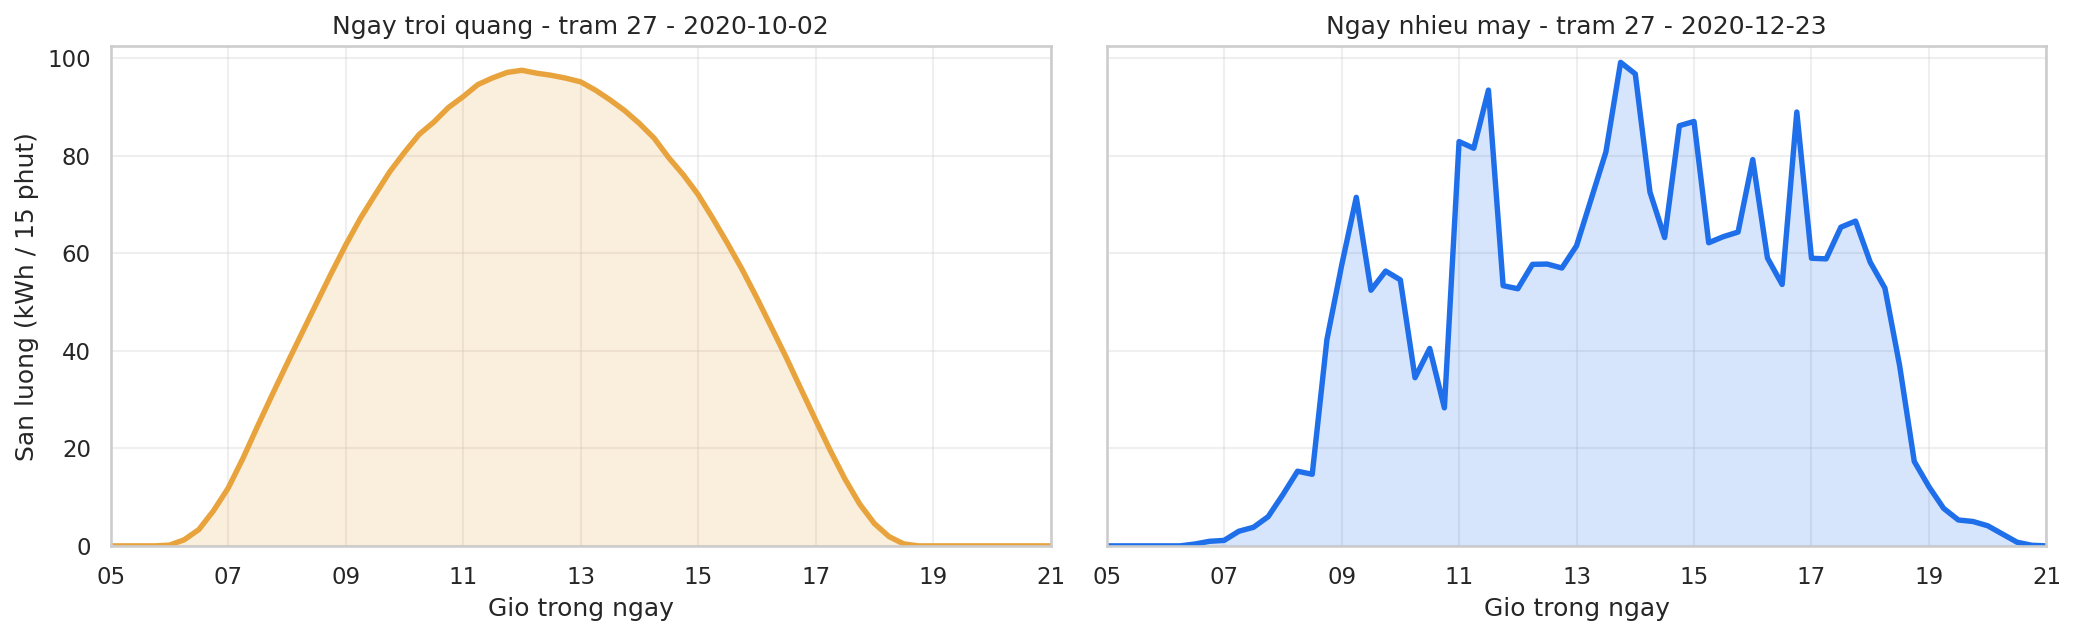
\includegraphics[width=\textwidth]{eda_mau_hinh_phat_dien.png}
    
    
    \caption{Đặc tuyến sản lượng ngày trời quang và ngày nhiều mây tại trạm 27}
    \label{fig:eda_mau_hinh}
\end{figure}

% Tieu de nay chi co mot cau roi den bang, de tu nhien thi no ket thuc trang mot minh.
% Con duoi 6 dong thi day ca cum sang trang moi.
\needspace{6\baselineskip}
\subsubsection{Tự tương quan}

Bảng~\ref{tab:eda_acf} ghi tự tương quan của chuỗi sản lượng
tại các mốc trễ đáng chú ý.

\begin{table}[htbp]
\centering
\caption{Hệ số tự tương quan (ACF) chuỗi sản lượng trạm $27$ tại các mốc trễ}
\label{tab:eda_acf}
\small
\begin{tabular}{l r r}
\toprule
\textbf{Mốc trễ} & \textbf{Khoảng cách} & \textbf{ACF} \\
\midrule
\texttt{lag\_1}   & $15$ phút  & $\mathbf{+0{,}9690}$ \\
\texttt{lag\_4}   & $1$ giờ    & $+0{,}9035$ \\
\texttt{lag\_96}  & $24$ giờ   & $+0{,}7134$ \\
--- & $48$ giờ & $+0{,}6614$ \\
--- & $72$ giờ & $+0{,}6466$ \\
\bottomrule
\end{tabular}


\end{table}

Con số $+0{,}9690$ tại mốc $15$ phút là điểm cần đọc kỹ. Ở mức tự tương quan đó, giá trị tại
$t$ gần như là bản sao của giá trị tại $t+1$, nên một mô hình được cấp \texttt{lag\_1} sẽ có lối
tắt hiển nhiên: lặp lại giá trị vừa đo. Mốc $1$ giờ vẫn giữ tương quan cao $+0{,}9035$ nhưng
đã đủ xa để không còn là bản sao, còn mốc $24$ giờ ở $+0{,}7134$ mang thông tin chu kỳ ngày.
Hình~\ref{fig:eda_acf} là biểu đồ đầy đủ.
Ba con số này là căn cứ định lượng cho lựa chọn trình bày ở Mục~\ref{subsec:dac_trung_thoi_gian}.

\begin{figure}[htbp]
    \centering
    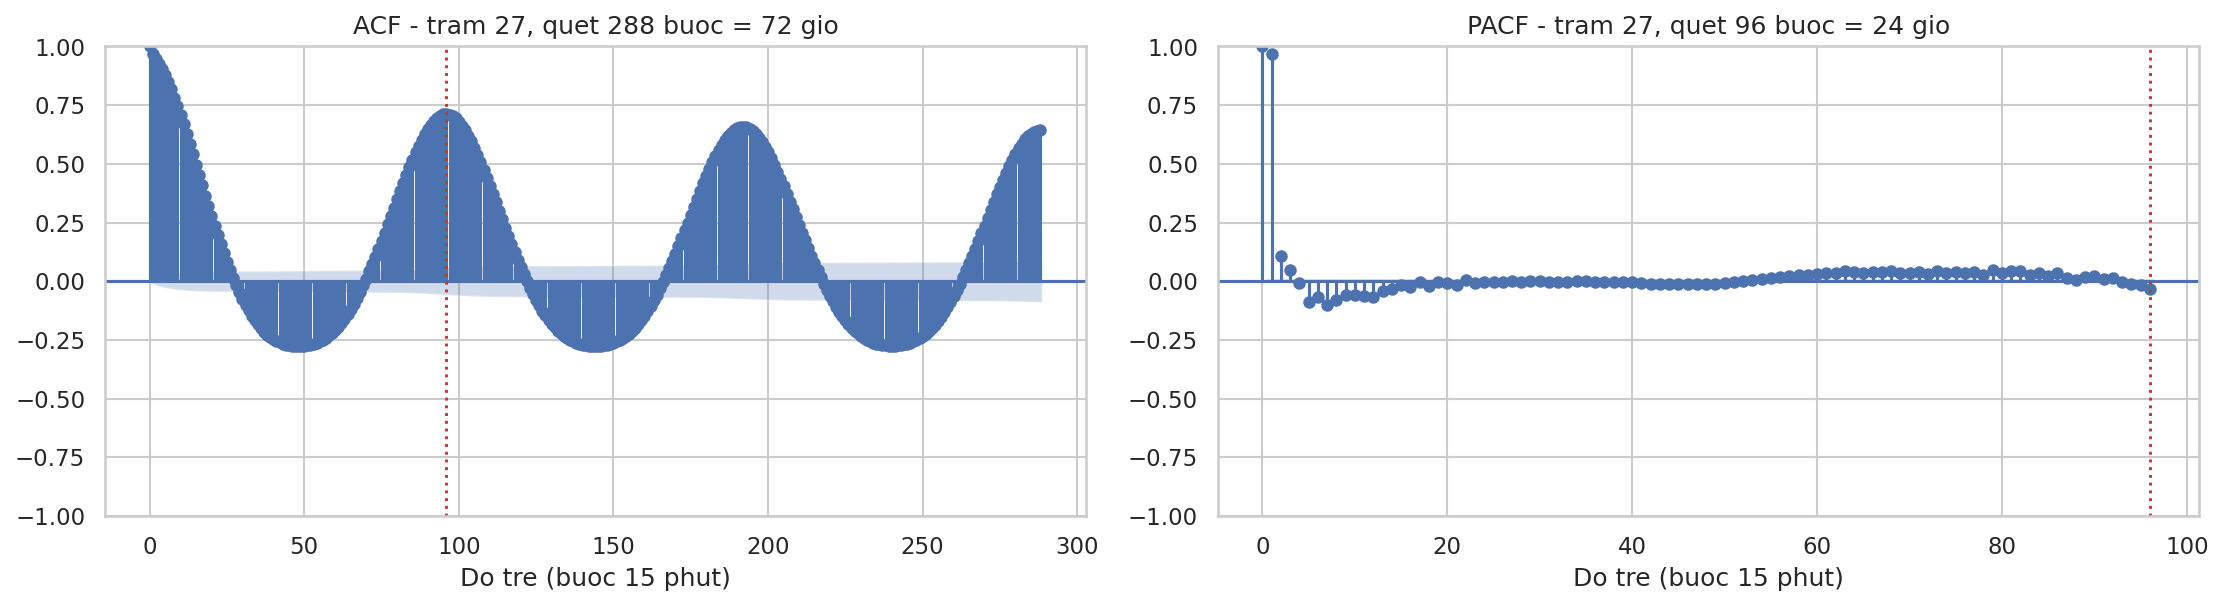
\includegraphics[width=\textwidth]{eda_acf_pacf.png}
    
    
    \caption{Biểu đồ tự tương quan ACF và tương quan riêng phần PACF}
    \label{fig:eda_acf}
\end{figure}

\subsubsection{Tương quan giữa các biến}

Tương quan tính trên $606.112$ dòng đo thật ban ngày, xem Bảng~\ref{tab:eda_tuong_quan}.

\begin{table}[htbp]
\centering
\caption{Tương quan giữa các biến khí tượng với sản lượng điện}
\label{tab:eda_tuong_quan}
\small
\begin{tabular}{l r r r}
\toprule
\textbf{Biến} & \textbf{Spearman ban ngày} & \textbf{Gộp cả đêm} & \textbf{Chênh} \\
\midrule
\texttt{shortwave\_radiation}      & $+0{,}6043$ & $+0{,}9112$ & $+0{,}3069$ \\
\texttt{direct\_normal\_irradiance} & $+0{,}5513$ & $+0{,}8877$ & $+0{,}3364$ \\
\texttt{diffuse\_solar\_radiation}  & $+0{,}3809$ & $+0{,}8837$ & $+0{,}5028$ \\
\texttt{temperature\_c}            & $+0{,}2639$ & $+0{,}4527$ & $+0{,}1888$ \\
\texttt{cloud\_cover\_total}        & $-0{,}1591$ & $+0{,}0280$ & $+0{,}1870$ \\
\bottomrule
\end{tabular}


\end{table}

Cột chênh lệch là kết quả đáng chú ý nhất của cả bước khảo sát. Nếu gộp cả ban đêm, tương
quan của \texttt{shortwave\_radiation} với sản lượng vọt từ $+0{,}60$ lên $+0{,}90$, và
\texttt{diffuse\_solar\_radiation} vọt từ $+0{,}38$ lên $+0{,}88$. Mức tăng đó không phản
ánh quan hệ vật lý: ban đêm mọi biến bức xạ và sản lượng đều bằng $0$ cùng lúc, nên hơn một
nửa số điểm nằm chồng tại gốc toạ độ và tự động đẩy hệ số tương quan lên.
Ma trận đầy đủ ở Hình~\ref{fig:eda_corr}.

Cột \texttt{cloud\_cover\_total} cho thấy rõ nhất: ban ngày nó mang dấu âm $-0{,}1591$ --- đúng ý nghĩa vật lý là mây che thì sản lượng giảm nhưng gộp cả đêm thì đổi thành dấu
dương $+0{,}0280$, tức đảo ngược hoàn toàn ý nghĩa. Vì vậy mọi tương quan trong tài liệu này
đều tính trên phạm vi đo thật ban ngày.

\begin{figure}[htbp]
    \centering
    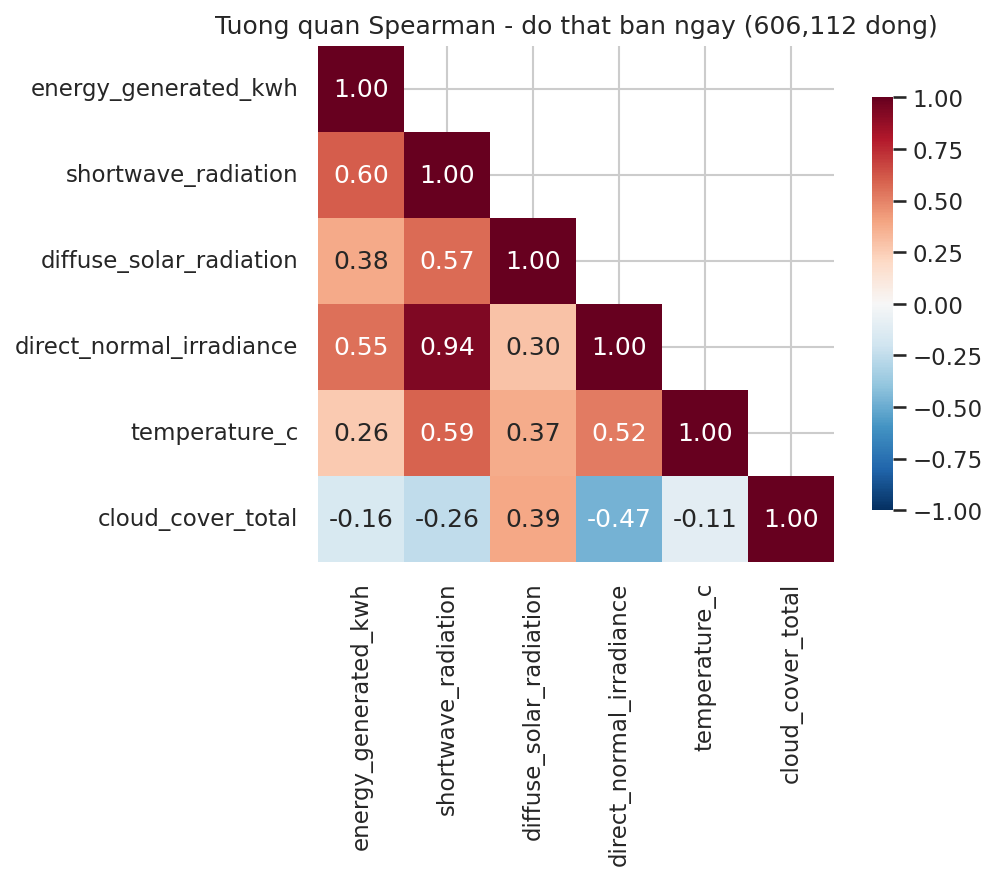
\includegraphics[width=0.78\textwidth]{eda_tuong_quan_spearman.png}
    
    
    \caption{Ma trận tương quan Spearman giữa các đặc trưng ban ngày}
    \label{fig:eda_corr}
\end{figure}

\FloatBarrier
\subsection{Chia dữ liệu theo trục thời gian}

Với bài toán dự báo, phép chia ngẫu nhiên thông thường là sai về nguyên tắc, vì cách chia đó cho
phép mô hình học từ dữ liệu của tháng sau rồi đi dự báo tháng trước. Notebook
\texttt{02\_split\_time\_series} vì vậy cắt dữ liệu \textbf{theo thứ tự thời gian}, không
xáo trộn.

Trước hết, $15\%$ số mốc thời gian cuối cùng được tách ra làm tập test niêm
phong và tách khỏi quy trình. Phần còn lại, gọi là tập Phát triển, mới được dùng để sinh đặc trưng,
chọn đặc trưng, tinh chỉnh siêu tham số (\textit{hyperparameter}) và chọn hàm mất mát. Tập test chỉ được mở đúng
một lần ở bước đánh giá cuối, sau khi mọi quyết định đã khoá.

Phép cắt thực hiện trên trục mốc thời gian, không phải trên số dòng. Toàn bộ dữ
liệu có $81.023$ mốc thời gian phân biệt; cắt $15\%$ cuối cho $12.154$ mốc thuộc tập test
và $68.869$ mốc thuộc tập Phát triển. Ranh giới rơi vào $18/12/2021$ lúc $09{:}30$:

\begin{itemize}
    \item \textbf{Tập Phát triển} --- từ $01/01/2020$ $00{:}15$ đến $18/12/2021$ $09{:}15$.
    \item \textbf{Tập test niêm phong} --- từ $18/12/2021$ $09{:}30$ đến $23/04/2022$ $23{:}45$.
\end{itemize}

Tỷ lệ $15\%$ tính trên mốc thời gian tương ứng $510.468$ dòng trên tổng $2.784.438$, tức
$18{,}33\%$ khối lượng dữ liệu. Hai tỷ lệ lệch nhau do số trạm hoạt động tăng dần
theo thời gian: đầu năm $2020$ có $30$ trạm phát sinh dữ liệu, tới cuối năm $2021$ đủ $42$
trạm, nên mỗi mốc thời gian ở giai đoạn sau mang nhiều dòng hơn giai đoạn trước.
Hình~\ref{fig:chia_du_lieu} mô tả cách chia.

Phép cắt theo mốc được chọn thay vì cắt theo số dòng vì nó cho một ranh giới thời gian duy
nhất áp dụng chung cho cả $42$ trạm. Cắt theo số dòng sẽ khiến mỗi trạm có một mốc cắt riêng
và tập test không còn là một giai đoạn liền mạch.

\begin{figure}[htbp]
    \centering
    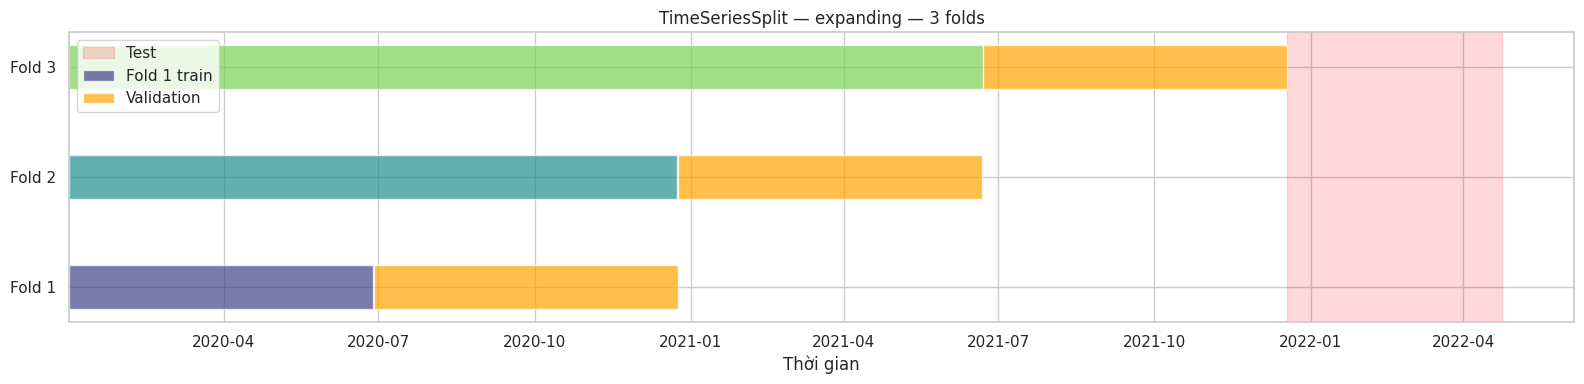
\includegraphics[width=\textwidth]{nb02_chia_du_lieu.png}
    
    
    \caption{Phân chia dữ liệu chuỗi thời gian theo cửa sổ mở rộng}
    \label{fig:chia_du_lieu}
\end{figure}

\FloatBarrier
\subsection{Ba fold theo cửa sổ mở rộng}

Tập Phát triển được chia thành ba fold theo kiểu cửa sổ mở rộng
(\textit{expanding window}): phần huấn luyện của fold sau chứa trọn phần huấn luyện lẫn
phần kiểm định của fold trước. Cách này mô phỏng đúng tình huống vận hành thật, càng
về sau càng có nhiều lịch sử để học, và bảo đảm phần kiểm định luôn nằm ở tương lai
so với phần huấn luyện.

Phép chia fold cũng thực hiện trên trục mốc thời gian, mỗi fold nhận đúng $17.217$ mốc cho
phần kiểm định, còn phần huấn luyện nới rộng dần qua $17.218$, $34.435$ rồi $51.652$ mốc.

\begin{table}[htbp]
\centering
\caption{Ranh giới thời gian, kích thước và số trạm của ba fold kiểm định}
\label{tab:ba_fold}
\small
\begin{tabular}{c l r c l r c}
\toprule
\textbf{Fold} & \multicolumn{3}{c}{\textbf{Phần huấn luyện}} & \multicolumn{3}{c}{\textbf{Phần kiểm định}} \\
\cmidrule(lr){2-4}\cmidrule(lr){5-7}
 & \textbf{đến} & \textbf{số dòng} & \textbf{trạm} & \textbf{đến} & \textbf{số dòng} & \textbf{trạm} \\
\midrule
$1$ & 28/06/2020 08:30 & $233.244$ & $30$ & 24/12/2020 16:45 & $606.105$ & $39$ \\
$2$ & 24/12/2020 16:45 & $839.349$ & $39$ & 22/06/2021 01:00 & $711.507$ & $42$ \\
$3$ & 22/06/2021 01:00 & $1.550.856$ & $42$ & 18/12/2021 09:15 & $723.114$ & $42$ \\
\bottomrule
\end{tabular}


\end{table}

Nhìn Bảng~\ref{tab:ba_fold} thấy rõ tính chất mở rộng: mốc kết thúc huấn luyện của fold
$2$ trùng đúng mốc kết thúc kiểm định của fold $1$, và tương tự giữa fold $3$ với fold
$2$. Kích thước tập huấn luyện tăng dần từ $233$ nghìn lên $1{,}55$ triệu dòng, trong
khi tập kiểm định giữ quy mô tương đương nhau, khoảng $600$--$720$ nghìn dòng.

Vì sao chọn cửa sổ mở rộng thay vì cửa sổ trượt. Hai cách chia đều tôn trọng
trục thời gian, khác nhau ở chỗ xử lý dữ liệu cũ. Cửa sổ mở rộng giữ lại toàn bộ quá khứ:
tập huấn luyện của fold sau chứa trọn tập huấn luyện của fold trước cộng thêm phần kiểm
định của nó, nên bề rộng lớn dần, ở đây là $233$ nghìn rồi $839$ nghìn rồi $1{,}55$ triệu
dòng. Cửa sổ trượt giữ bề rộng cố định và đẩy cả hai đầu về phía trước, tức mỗi lần tiến
một bước thì cắt bỏ một đoạn đầu tương ứng.

Ba lý do khiến cửa sổ mở rộng phù hợp với bài toán này. Thứ nhất, dữ liệu chỉ trải hơn
hai năm trong khi chu kỳ chi phối sản lượng là chu kỳ mùa dài đúng một năm; cửa sổ trượt
với bề rộng cố định sẽ khiến fold đầu tiên chỉ nhìn thấy vài tháng, không đủ trọn một
vòng mùa để học được dạng đường cong ngày của cả mùa hè lẫn mùa đông. Thứ hai, các trạm
lần lượt đi vào vận hành theo thời gian, từ $30$ trạm ở fold $1$ lên $42$ trạm ở fold $3$;
cắt bỏ đoạn đầu đồng nghĩa vứt luôn phần lịch sử sớm của những trạm vận hành trước, trong
khi đó lại chính là phần dữ liệu dài nhất của chúng. Thứ ba, quan hệ giữa bức xạ và sản
lượng của tấm quang điện là quan hệ vật lý, không đổi nhanh theo thời gian, nên dữ liệu
cũ vẫn còn giá trị mô tả.

Cửa sổ trượt sẽ là lựa chọn tốt hơn khi hệ thống có trôi khái niệm mạnh, chẳng hạn thay
tấm pin, đổi biến tần hay đổi cấu hình lắp đặt, vì khi đó dữ liệu cũ mô tả một hệ thống
khác và trở thành nhiễu. Bộ dữ liệu này không có sự kiện như vậy.

Đánh đổi phải chấp nhận là ba fold không cùng cỡ tập huấn luyện, nên sai số của từng fold
không so trực tiếp với nhau được: fold $1$ vừa ít dữ liệu vừa vướng vấn đề trạm mới nêu
ngay dưới đây. Vì vậy tài liệu chỉ dùng WAPE gộp ba fold để xếp hạng cấu hình, không đọc
riêng con số của một fold.

Hạn chế: fold sớm có trạm chưa từng xuất hiện khi huấn luyện. Cột số trạm trong
Bảng~\ref{tab:ba_fold} cho thấy một hệ quả trực tiếp của việc các trạm lần lượt đi vào vận
hành theo thời gian. Ở fold $1$, mô hình học trên $30$ trạm nhưng bị chấm điểm trên $39$
trạm; ở fold $2$ là $39$ trạm so với $42$. Chênh lệch đó nghĩa là một phần dữ liệu kiểm định
thuộc về những trạm mà mô hình chưa từng nhìn thấy một dòng nào lúc huấn luyện. Tới
fold $3$ thì cả $42$ trạm đều đã có mặt ở phần huấn luyện nên tình huống này không còn.

Ảnh hưởng của nó làm sai số đo trên fold $1$ và fold $2$ bi quan hơn thực tế vận
hành, vì trong vận hành thật mô hình luôn đã có lịch sử của trạm mà nó dự báo. Chiều ảnh
hưởng là an toàn, sai số bị đánh giá nặng hơn chứ không nhẹ đi, nhưng khi so sánh các
cấu hình bằng WAPE gộp ba fold thì phần đóng góp của fold $1$ vẫn mang theo thành phần sai
lệch này.

\FloatBarrier
\subsection{Thực nghiệm: đo phần chồng lấn nhãn ở ranh giới fold}

Ba fold được cắt liên tục, không chèn khoảng đệm giữa phần huấn luyện và phần kiểm
định. Hai quy tắc chống rò rỉ nêu ở Mục~\ref{subsec:so_do_toan_canh} chỉ ràng buộc đặc trưng đầu
vào; riêng nhãn cần một phép kiểm riêng. Nhãn của một dòng huấn luyện là sản
lượng tại $T + h$, nên với những dòng nằm sát mốc cắt, thời điểm $T + h$ có thể đã rơi
sang vùng kiểm định. Nhóm đo trực tiếp phần chồng lấn này.

Cách tiến hành. Với mỗi fold, đọc trực tiếp tệp
\texttt{fold\_i\_train\_selected.parquet}, lấy mốc thời gian lớn nhất $T_{\max}$ của phần
huấn luyện. Một dòng có nhãn rơi sang vùng kiểm định khi và chỉ khi mốc thời gian của dòng đó lớn hơn
$T_{\max} - 15h$ phút, với $h$ là số bước của tầm dự báo. Đếm số dòng thoả điều kiện đó
cho cả hai tầm H1 và H4. Phép đo chạy trên chính các tệp fold mà bước huấn luyện đọc
vào, không dùng dữ liệu trung gian nào khác.

\begin{table}[htbp]
\centering
\caption{Kiểm tra hiện tượng chồng lấn nhãn giữa các fold}
\label{tab:chong_lan}
\small
\begin{tabular}{c r r r r}
\toprule
\textbf{Fold} & \textbf{Cỡ tập huấn luyện} & \textbf{Chồng lấn H1} & \textbf{Chồng lấn H4} & \textbf{Tỷ lệ H4} \\
\midrule
$1$ & $233.244$ & $30$ & $120$ & $0{,}0514\%$ \\
$2$ & $839.349$ & $39$ & $156$ & $0{,}0186\%$ \\
$3$ & $1.550.856$ & $42$ & $168$ & $0{,}0108\%$ \\
\bottomrule
\end{tabular}


\end{table}

Trường hợp xấu nhất là fold $1$ ở tầm H4: $120$ dòng trên $233.244$, tức
$\mathbf{0{,}0514\%}$. Tỷ lệ nhỏ như vậy là hệ quả cấu trúc của phép cắt, chỉ những dòng
nằm trong $h$ bước cuối cùng của tập huấn luyện mới có nhãn vượt sang vùng kiểm định, mà
$h$ nhiều nhất là bốn bước.

Bảng~\ref{tab:chong_lan} tự kiểm chứng được. Ở tầm H1 chỉ một bước cuối bị chồng
lấn, nên số dòng phải bằng số trạm còn hoạt động tại bước đó: cột chồng lấn H1 cho $30$,
$39$ và $42$, tương ứng với cột số trạm ở Bảng~\ref{tab:ba_fold}. Cột H4 bằng bốn lần các
giá trị đó.

Với mức chồng lấn dưới một phần nghìn ở cả ba fold, phép cắt liên tục được giữ nguyên,
không chèn khoảng đệm.

\FloatBarrier
\section{Sinh đặc trưng}

Ba notebook liên tiếp bổ sung đặc trưng vào cùng một khung dữ liệu, mỗi notebook phụ trách
một họ: \texttt{03\_1\_features\_time} sinh đặc trưng suy từ trục thời gian và từ lịch sử sản
lượng, \texttt{03\_2\_features\_spatial} sinh đặc trưng hình học Mặt Trời cùng các đại lượng chuẩn
hoá theo trạm, \texttt{03\_3\_features\_aggregate} sinh đặc trưng tương tác khí tượng và mã hoá
biến phân loại. Hai notebook sau đó thu hẹp lại: \texttt{04\_vif\_diagnostics} chẩn đoán đa cộng
tuyến, \texttt{05\_select\_features} chốt danh sách chính thức.

\FloatBarrier
\subsection{Đặc trưng thời gian, trễ và cửa sổ trượt}
\label{subsec:dac_trung_thoi_gian}

Notebook \texttt{03\_1\_features\_time} sinh ba nhóm đặc trưng, tóm tắt ở
Bảng~\ref{tab:dac_trung_thoi_gian}.

\begin{table}[htbp]
\centering
\caption{Các nhóm đặc trưng thời gian và độ trễ}
\label{tab:dac_trung_thoi_gian}
\small
\begin{tabular}{@{}L{2.8cm} L{6.6cm} L{4.7cm}@{}}
\toprule
\textbf{Nhóm} & \textbf{Cột sinh ra} & \textbf{Tham số} \\
\midrule
Lịch và chu kỳ &
\texttt{minute\_of\_day}, \texttt{month}, \texttt{day\_of\_week}, \texttt{is\_weekend},
\texttt{season}, \texttt{season\_code}, \texttt{hour\_sin}, \texttt{hour\_cos},
\texttt{doy\_sin}, \texttt{doy\_cos} &
chu kỳ ngày $1440$ phút; chu kỳ năm $365{,}25$ ngày \\
\addlinespace
Trễ &
\texttt{lag\_4}, \texttt{lag\_96} &
\texttt{LAGS} $= (4,\ 96)$, tức $T - 60$ phút và $T - 24$ giờ \\
\addlinespace
Cửa sổ trượt &
\texttt{rolling\_mean}, \texttt{rolling\_std}, \texttt{rolling\_min},
\texttt{rolling\_max} cho mỗi cửa sổ &
\texttt{ROLLING\_WINDOWS} $= (4,\ 96)$, bốn thống kê mỗi cửa sổ \\
\bottomrule
\end{tabular}


\end{table}

Nhóm lịch và chu kỳ sinh ra $10$ cột ở bước này, nhưng chỉ $5$ cột đi tiếp vào bộ đặc trưng
cuối sau bước chọn ở Mục~\ref{subsec:chan_doan_dac_trung}. Hai nhóm sau tạo ra $2$ cột trễ cộng
$8$ cột cửa sổ trượt, bằng $10$ cột suy từ chuỗi mục
tiêu, đúng con số notebook in ra khi khai báo hàm sinh đặc trưng.

Mã hoá lịch bằng sin và cos. Nếu để giờ trong ngày ở dạng số nguyên, mốc $23{:}45$
và mốc $00{:}00$ cách nhau đúng một bước $15$ phút trên thực tế nhưng cách nhau $23$ đơn vị
trên thang số. Cây quyết định chia theo ngưỡng sẽ coi hai mốc liền kề đó là hai vùng xa
nhau. Cặp $(\sin, \cos)$ đưa trục thời gian về một vòng tròn khép kín, nên khoảng cách giữa
hai mốc kề nhau qua nửa đêm trở lại đúng bằng khoảng cách thật. Cùng lý do, ngày trong năm
được mã hoá bằng \texttt{doy\_sin} và \texttt{doy\_cos} theo chu kỳ $365{,}25$ ngày.

\subsubsection{Thực nghiệm: chọn mốc trễ}

Khái niệm nền. \textit{Persistence} là mô hình dự báo cơ sở: lấy giá trị quan sát
tại $t$ làm dự báo cho $t+h$. Dev và cộng sự~\cite{dev2018tes} định nghĩa nó là phương pháp
\textit{giả định điều kiện tại thời điểm dự báo không thay đổi so với thời điểm quan sát},
và ghi nhận rằng cách này \textit{chạy tốt} ở các tầm dự báo ngắn, khi điều kiện thời tiết
biến thiên chậm:

\begin{quote}\small
\textit{``The persistence forecasting method assumes that the conditions for the forecast do not change (especially for shorter lead times). This method works well in conditions when weather maps change very slowly with time.''}
\end{quote}


Từ định nghĩa trên suy ra một hệ quả đại số mà bài báo không nêu: nếu $\hat{y}(t+h) = y(t)$
thì đường dự báo chính là đường đo thật dịch phải $h$ bước, tức lệch pha đúng bằng
tầm dự báo. Mặt khác, vì chuỗi biến thiên chậm ở tầm ngắn, đúng điều kiện mà bài báo nói
\textit{persistence} chạy tốt, nên hiệu giữa $y(t)$ và $y(t+h)$ nhỏ, và một chỉ số sai số
tính theo từng điểm vẫn cho con số đẹp.

Tầm H1 của dự án đúng bằng $15$ phút, nằm trọn trong vùng đó. Một mô hình lặp lại giá trị vừa
đo sẽ cho chỉ số sai số tốt nhưng đường dự báo trễ một nhịp, con số đẹp
ở đây không chứng minh năng lực dự báo.

Giả thuyết. Mốc trễ càng gần thời điểm dự báo thì tín hiệu càng mạnh, nhưng cũng
càng dễ kéo mô hình về đúng dạng vừa nêu. Thực nghiệm này xác định mốc trễ nào được đưa vào.

Cách tiến hành. Ba cấu hình được đối chiếu trên cùng dữ liệu và cùng quy trình tinh
chỉnh: cấu hình nền chỉ có \texttt{lag\_96} ($T - 24$ giờ), cấu hình thêm \texttt{lag\_1}
($T - 15$ phút), và cấu hình thêm \texttt{lag\_4} ($T - 60$ phút). Mỗi cấu hình được chấm
bằng WAPE và một phép đo lệch pha riêng: độ trễ trung bình giữa đường dự báo và
đường đo thật trên từng trạm, kèm số trạm vượt ngưỡng cho phép. Ba mốc đã thử ghi ở
Bảng~\ref{tab:chon_lag}.

\begin{table}[htbp]
\centering
\caption{Lựa chọn các mốc trễ chuỗi thời gian}
\label{tab:chon_lag}
\small
\begin{tabular}{@{}L{3.4cm} L{3.6cm} L{7.0cm}@{}}
\toprule
\textbf{Mốc trễ} & \textbf{Quyết định} & \textbf{Căn cứ ghi trong notebook} \\
\midrule
\texttt{lag\_96} ($T-24$ giờ) & \textbf{giữ} &
Chu kỳ ngày; xa thời điểm dự báo nên không tạo lệch pha \\
\addlinespace
\texttt{lag\_1} ($T-15$ phút) & \textbf{loại} &
Gây lệch pha trên gần như toàn bộ đội hình; sai số theo từng điểm giảm nhưng là hệ quả của
việc lặp lại giá trị vừa đo \\
\addlinespace
\texttt{lag\_4} ($T-60$ phút) & \textbf{giữ} &
Đủ xa để không lặp lại được giá trị vừa đo, vẫn đủ gần để mang thông tin quán tính; qua được
cổng lệch pha ở Mục~\ref{subsec:dac_trung_thoi_gian} \\
\bottomrule
\end{tabular}


\end{table}

Đọc kết quả. Quyết định phân biệt \texttt{lag\_1} với \texttt{lag\_4} không dựa vào
sai số mà dựa vào lệch pha. Nếu chỉ nhìn WAPE thì \texttt{lag\_1} sẽ được chọn, vì
nó cho con số thấp nhất, đúng như hệ quả đại số nêu ở đầu mục. Dự án chốt \texttt{LAGS}
$= (4,\ 96)$ và loại \texttt{lag\_1}.

Giới hạn của bằng chứng này: notebook ghi lại quyết định và căn cứ định tính, không lưu một
phép đối chứng có kiểm soát giữa ba cấu hình trên cùng một lần chạy.

\subsubsection{Cổng lệch pha đặt trước bước tinh chỉnh}

Phép đo lệch pha được đặt thành một cổng chặn ở đầu notebook huấn luyện: chỉ khi cổng đạt
thì quy trình mới được phép chạy Optuna và huấn luyện thật.

Độ trễ suy từ quan hệ giữa sai số và độ dốc của đường đo thật. Nếu đường dự báo bị dịch
$c$ bước thì sai số xấp xỉ $-c$ nhân với độ dốc, nên hệ số hồi quy của sai số theo độ dốc
chính là $c$:

\begin{equation}
\text{độ trễ (phút)} \;=\; -\,\frac{\sum_t d_t \, e_t}{\sum_t d_t^{2}} \times 15,
\qquad
d_t = \frac{y_{t+1} - y_{t-1}}{2}, \quad e_t = \hat{y}_t - y_t .
\end{equation}

Cách này tách sai số biên độ khỏi sai số thời điểm: dự báo cao hơn hay thấp hơn thực tế
đều không làm đổi con số, chỉ việc đến sớm hay đến muộn mới làm đổi.

Ngưỡng và kết quả. Cổng yêu cầu độ trễ nằm trong $\pm 5$ phút và không trạm nào vượt
ngưỡng. Kết quả in ra ở notebook \texttt{06\_1\_train\_mae}:

% Khoi ket xuat notebook. Khong boc trong minipage nua: minipage la mot hop lien
% khoi, khong the ngat trang, nen khoi dai bi day nguyen sang trang sau va de lai
% khoang trong lon. De verbatim o muc doan van thi no tu ngat duoc.
\begingroup
\par\vspace{6pt}\hrule\vspace{4pt}
\small\renewcommand{\baselinestretch}{1.0}\selectfont
\begin{verbatim}
TRAIN THU NHANH DE DO TRE (truoc khi tune)
Train thu 300,000 dong x 52 dac trung trong 10.2 giay

TREN 288,136 diem ban ngay cua tap VALIDATION:
   Do tre        : +2.38 phut   (duong = du bao di SAU thuc te)
   Nguong cho phep: +/- 5.0 phut
   WAPE tham khao : 22.07%  (model nho, chua tune - chi de doi chieu)

Site vuot nguong: 0/40
Tre theo site: trung vi +2.56 phut | nho nhat -0.62 | lon nhat +3.99

CONG DO TRE: DAT - tre +2.38 phut, khong site nao vuot nguong.
Cho phep chay Optuna va train that.
\end{verbatim}
\vspace{2pt}\hrule\par\vspace{6pt}
\endgroup

Mô hình dùng ở cổng. Cổng chạy trên một mô hình nháp, cùng thuật toán và cùng hàm
mất mát với mô hình cuối nhưng nhỏ hơn nhiều, xem Bảng~\ref{tab:mo_hinh_nhap}.

\begin{table}[htbp]
\centering
\caption{So sánh cấu hình mô hình nháp và mô hình chính thức}
\label{tab:mo_hinh_nhap}
\small
\begin{tabular}{@{}L{4.6cm} L{4.9cm} L{4.6cm}@{}}
\toprule
 & \textbf{Mô hình nháp (cổng)} & \textbf{Mô hình cuối} \\
\midrule
Thuật toán & LightGBM & LightGBM \\
Hàm mất mát & \texttt{l1} (MAE) & \texttt{l1} (MAE) \\
Số đặc trưng & $52$ & $52$ \\
Trọng số mẫu & có & có \\
\addlinespace
Quy mô tập đầu vào & $300.000$ lấy ngẫu nhiên & $1.550.856$ \\
Số cây & $200$, đặt cố định & Optuna chọn \\
Tốc độ học & $0{,}08$, đặt cố định & Optuna chọn \\
\texttt{num\_leaves} & $63$, đặt cố định & Optuna chọn \\
Thời gian huấn luyện & $10{,}2$ giây & hàng chục phút \\
\bottomrule
\end{tabular}


\end{table}

Vì thuật toán, hàm mất mát và danh sách đặc trưng thống nhất với mô hình cuối, cổng kiểm được đúng
thứ nó cần kiểm: bộ đặc trưng có đẩy mô hình vào hành vi bám trụ hay không. Nếu
\texttt{lag\_1} có mặt thì mô hình nháp cũng sao chép giá trị gần nhất y như mô hình cuối.

Ngưỡng là $\pm 5$ phút và không trạm nào được vượt. Đo trên $288.136$ điểm ban ngày, độ
trễ là $+2{,}38$ phút, trung vị theo trạm $+2{,}56$ phút, dao động từ $-0{,}62$ đến
$+3{,}99$, và $0/40$ trạm vượt ngưỡng, nên cổng đạt. Cổng này đặt trước bước tinh chỉnh
nên chỉ kiểm bộ đặc trưng; sau khi Optuna chọn xong siêu tham số (\textit{hyperparameter}), notebook chạy tiếp một
phép quét độ trễ thứ hai trên toàn bộ tập kiểm định, trình bày ở phần đánh giá.

\subsubsection{Rào chắn chống rò rỉ và ngữ cảnh lùi}

Bước sinh đặc trưng đặt hai rào chắn. Một, mọi đặc trưng suy từ mục tiêu đều được dịch:
các cột cửa sổ trượt tính trên chuỗi mục tiêu đã dịch một bước, nên giá trị tại $T$ không
bao giờ chứa sản lượng đo tại chính $T$. Hai, một mặt nạ lịch sử liên tục kiểm tra toàn
bộ số bước của cửa sổ liền trước đều cách nhau đúng $15$ phút; cửa sổ vắt qua chỗ đứt gãy
thì bị gán khuyết thay vì tính bừa trên hai đoạn không liền nhau.

Ngữ cảnh lùi giải quyết vế còn lại: mỗi tập được nối thêm lịch sử của tập liền trước
trước khi tính đặc trưng, rồi chỉ xuất phần dòng thuộc chính tập đó. Tập test dùng toàn
bộ tập Phát triển làm ngữ cảnh, tập kiểm định dùng tập huấn luyện, và phần kiểm định của
mỗi fold dùng phần huấn luyện của chính fold đó. Nhờ vậy dòng đầu tiên của mỗi tập vẫn có
đủ lịch sử, mà mỗi fold vẫn là một thí nghiệm khép kín.

Kết quả thực thi. Khối dưới đây trích nguyên văn kết quả kết xuất của notebook
\texttt{03\_1\_features\_time}:

% Khoi ket xuat notebook. Khong boc trong minipage nua: minipage la mot hop lien
% khoi, khong the ngat trang, nen khoi dai bi day nguyen sang trang sau va de lai
% khoang trong lon. De verbatim o muc doan van thi no tu ngat duoc.
\begingroup
\par\vspace{6pt}\hrule\vspace{4pt}
\footnotesize\renewcommand{\baselinestretch}{1.0}\selectfont
\begin{verbatim}
So dac trung target se tao: 2 lag + 8 rolling = 10 cot

Da sinh dac trung thoi gian cho development va test
(da ghi file va giai phong RAM).
- development: 2273970 dong x 74 cot
- test       : 510468 dong x 75 cot

Da sinh dac trung thoi gian cho train/val (da ghi file va giai phong RAM).
- train_alias: 1550856 dong x 75 cot
- val_alias  : 723114 dong x 75 cot

fold_1: train 233244 dong | val 606105 dong | 76 cot
fold_2: train 839349 dong | val 711507 dong | 76 cot
fold_3: train 1550856 dong | val 723114 dong | 76 cot

Số lượng NaN trong các tập:
- Train: 21000 (Đã dropna ở bước 7)
- Val:   0
- Test:  0

0 điểm đứt gãy - lưới thời gian liên tục 100% nhờ Reindex Notebook 01.
(Tổng số dòng: 1550856)
\end{verbatim}
\vspace{2pt}\hrule\par\vspace{6pt}
\endgroup

Ô khuyết chỉ xuất hiện ở tập huấn luyện, tại các dòng đầu chuỗi chưa đủ $96$ bước lịch sử
để tính cửa sổ dài. Tập kiểm định và tập test không còn ô khuyết nào nhờ ngữ cảnh lùi.

\FloatBarrier
\subsection{Solar geometry, bức xạ trời quang và chuẩn hoá theo trạm}
\label{subsec:solar_geometry}

Notebook \texttt{03\_2\_features\_spatial} sinh nhóm đặc trưng suy từ vị trí Mặt Trời, còn
\texttt{03\_3\_features\_aggregate} sinh nhóm tương tác khí tượng và mã hoá biến phân loại. Cả hai
nhóm đều là hàm xác định của thời gian và vị trí hoặc là tổ hợp của các biến đã có,
nên không mang rủi ro rò rỉ.

\subsubsection{Vị trí Mặt Trời: từ thuật toán NOAA sang pvlib SPA}

Bản dựng đầu tiên tính góc cao $h$ và góc phương vị bằng thuật toán vị trí Mặt Trời của
NOAA~\cite{noaa_solar}, dựa trên chuỗi Fourier cho độ xích vĩ, phương trình thời gian và
góc giờ. Cách làm đó cho kết quả đủ dùng nhưng vướng một điểm yếu ở khâu quy đổi múi giờ.
Bản hiện hành thay bằng hàm
\texttt{pvlib.solarposition.get\_solarposition} của thư viện \texttt{pvlib}
phiên bản \texttt{0.15.2}~\cite{holmgren2018pvlib}, tức thuật toán SPA của Reda và
Andreas, đồng thời lấy lịch giờ mùa hè thật của múi \texttt{Australia/Melbourne} thay cho
quy ước cắt theo nguyên tháng.

Ba chi tiết cài đặt đáng nêu, tóm tắt ở Bảng~\ref{tab:chi_tiet_solar}.

\begin{table}[htbp]
\centering
\caption{Chi tiết cài đặt các tham số hình học Mặt Trời}
\label{tab:chi_tiet_solar}
\small
\begin{tabular}{@{}L{2.8cm} L{5.4cm} L{6.4cm}@{}}
\toprule
\textbf{Chi tiết} & \textbf{Trong mã nguồn} & \textbf{Lý do} \\
\midrule
Quy đổi về giờ UTC &
\texttt{ZoneInfo('Australia/}\allowbreak\texttt{Melbourne')} tra đúng lịch giờ mùa hè cho
từng mốc &
Mốc trong dữ liệu là giờ địa phương của Úc, còn công thức thiên văn cần giờ UTC.
Bản trước dùng quy ước $11$ giờ cho tháng $10$--$3$ và $10$ giờ cho tháng $4$--$9$ \\
\addlinespace
Góc phương vị &
\texttt{np.arctan2(...)} thay cho $\arccos$ &
$\arccos$ chỉ trả về miền $[0^\circ;\ 180^\circ]$ nên không phân biệt được buổi sáng với
buổi chiều; $\operatorname{atan2}$ liên tục trên trọn vòng $360^\circ$ \\
\addlinespace
Dạng vòng của góc &
\texttt{azimuth\_sin}, \texttt{azimuth\_cos} &
Góc đo bằng độ gián đoạn ở mốc $0^\circ$ và $360^\circ$: $359^\circ$ và $1^\circ$ kề nhau
thực tế nhưng cách xa trên thang số \\
\bottomrule
\end{tabular}


\end{table}

Giờ mùa hè ở Úc bắt đầu Chủ nhật đầu tiên của tháng $10$ và kết thúc Chủ nhật đầu tiên của
tháng $4$, không rơi đúng vào ranh giới tháng, nên quy ước cắt theo nguyên tháng gán sai một
giờ cho khoảng $12$ ngày mỗi năm. Quy trình vì vậy chuyển sang \texttt{pvlib} và lịch múi giờ
thật, cho kết quả trùng khít thư viện chuẩn thay vì một bản cài đặt riêng.

\subsubsection{Bức xạ trời quang theo mô hình Haurwitz}

\textbf{GHI} (\textit{Global Horizontal Irradiance}) là tổng bức xạ Mặt Trời chiếu
xuống một mặt phẳng nằm ngang, đơn vị W/m\textsuperscript{2}. Nó gồm hai thành phần cộng
lại: phần trực xạ đi thẳng từ đĩa Mặt Trời và phần khuếch tán do bầu khí quyển và mây tán
xạ. Trong dữ liệu của dự án, hai đại lượng này nằm ở hai cột khác nhau và không được
lẫn:

\begin{itemize}
    \item \texttt{shortwave\_radiation} --- GHI lấy từ Open-Meteo, tức sản phẩm tái phân tích khí tượng chứ không phải cảm biến đặt tại trạm.
    \item \texttt{ghi\_cs} --- $GHI_{cs}$, giá trị lý thuyết khi trời hoàn toàn quang, do nhóm
    tự tính bằng mô hình Haurwitz từ góc cao Mặt Trời.
\end{itemize}

Vì $GHI_{cs}$ ứng với điều kiện không mây, nó là mức trần mà bức xạ đo được chỉ có thể tiệm
cận chứ không nên vượt qua.

Từ góc cao suy ra bức xạ ngang trời quang:

\begin{equation}
GHI_{cs} = 1098 \times \sin(h) \times \exp\!\left(-\frac{0{,}059}{\sin(h)}\right)
\quad (\mathrm{W/m^2})
\end{equation}

Cặp hằng số $1098$ và $0{,}059$ lấy đúng bản cài đặt Haurwitz của thư viện \texttt{pvlib},
vốn dẫn về hai bài gốc của Haurwitz~\cite{haurwitz1945}. Phần tóm tắt của bài báo
nguồn phát biểu dạng công thức như sau:

\begin{quote}\small
\textit{``These relations are of the form $T = (a/m)e^{-bm}$ where $m$ = air mass (i.e. secant of zenith distance of the sun), $e$ = base of natural logarithms, $a$ and $b$ are constants which depend on the cloudiness and cloud density.''}
\end{quote}


Mô hình trời quang thuần thiên văn ước lượng thiếu so với bức xạ đo tại các trạm, nên
$GHI_{cs}$ được nhân thêm hệ số hiệu chỉnh riêng từng trạm, đặt tên \texttt{cs\_factor}. Hệ số
này tính riêng trên phần huấn luyện của từng fold, xem Bảng~\ref{tab:cs_factor}.

\begin{table}[htbp]
\centering
\caption{Hệ số hiệu chỉnh trời quang \texttt{cs\_factor} theo từng fold}
\label{tab:cs_factor}
\small
\begin{tabular}{l r r r}
\toprule
\textbf{Phạm vi tính} & \textbf{Trung vị} & \textbf{Nhỏ nhất} & \textbf{Lớn nhất} \\
\midrule
Phần huấn luyện fold $1$ & $1{,}450$ & $1{,}098$ & $1{,}803$ \\
Phần huấn luyện fold $2$ & $1{,}541$ & $1{,}515$ & $1{,}825$ \\
Phần huấn luyện fold $3$ & $1{,}559$ & $1{,}538$ & $1{,}800$ \\
\bottomrule
\end{tabular}


\end{table}

Giá trị đổi giữa các fold, trung vị từ $1{,}450$ lên $1{,}559$, nên việc dùng chung
một bộ thống kê cho cả ba fold sẽ đưa thông tin của giai đoạn sau vào fold sớm. Notebook ghi
thẳng nguyên tắc này ở ô kết quả: \textit{mỗi fold dùng thống kê quy mô tính riêng từ tập
train của chính fold đó}.

\subsubsection{Thực nghiệm: hạ độ hạt bức xạ từ một giờ về mười lăm phút}

Vấn đề. Dữ liệu khí tượng có tần suất một giờ, còn lưới sản lượng có tần suất $15$
phút, nên mỗi giá trị bức xạ lặp lại bốn lần liên tiếp: trong một giờ, đặc trưng bức xạ không
phân biệt được mốc $12{:}00$ với mốc $12{:}15$.

Nguyên lý. Bailey và cộng sự~\cite{bailey2024} mô tả thuật toán của Graham và
Hollands ($1990$): tách chỉ số trời quang theo giờ $k_t$ thành mô hình cộng
$k_t = k_{tm} + \alpha$ gồm thành phần xu thế và thành phần nhiễu. Điểm cốt lõi là hạ độ hạt
của chỉ số trời quang chứ không phải bức xạ, vì bức xạ mang cả nhịp lên xuống theo góc Mặt
Trời trong ngày, còn chỉ số trời quang đã khử nhịp đó.

Dự án giữ đúng thành phần xu thế $k_{tm}$, giữ chỉ số trời quang không đổi trong mỗi khối
giờ rồi nhân lại với $GHI_{cs}$ tính ở từng mốc $15$ phút, và bỏ thành phần nhiễu $\alpha$,
vì $\alpha$ dùng để sinh chuỗi tổng hợp, còn ở đây bức xạ là đặc trưng đầu vào cho mô hình
dự báo.

Kết quả đo. Thước đo là tỷ lệ bước có giá trị bức xạ thay đổi so với bước liền trước, tính
riêng trên $750.564$ dòng ban ngày của tập huấn luyện. Trước khi hạ độ hạt, tỷ lệ này là
$26{,}7\%$~--- đúng như dự đoán, vì mỗi giá trị theo giờ lặp bốn lần nên cứ bốn bước mới có
một bước đổi giá trị. Sau khi hạ độ hạt, tỷ lệ lên $76{,}7\%$, tăng gần ba lần.
Hình~\ref{fig:downscale} cho thấy hiệu quả trên một cửa sổ sáu giờ.

\begin{figure}[htbp]
    \centering
    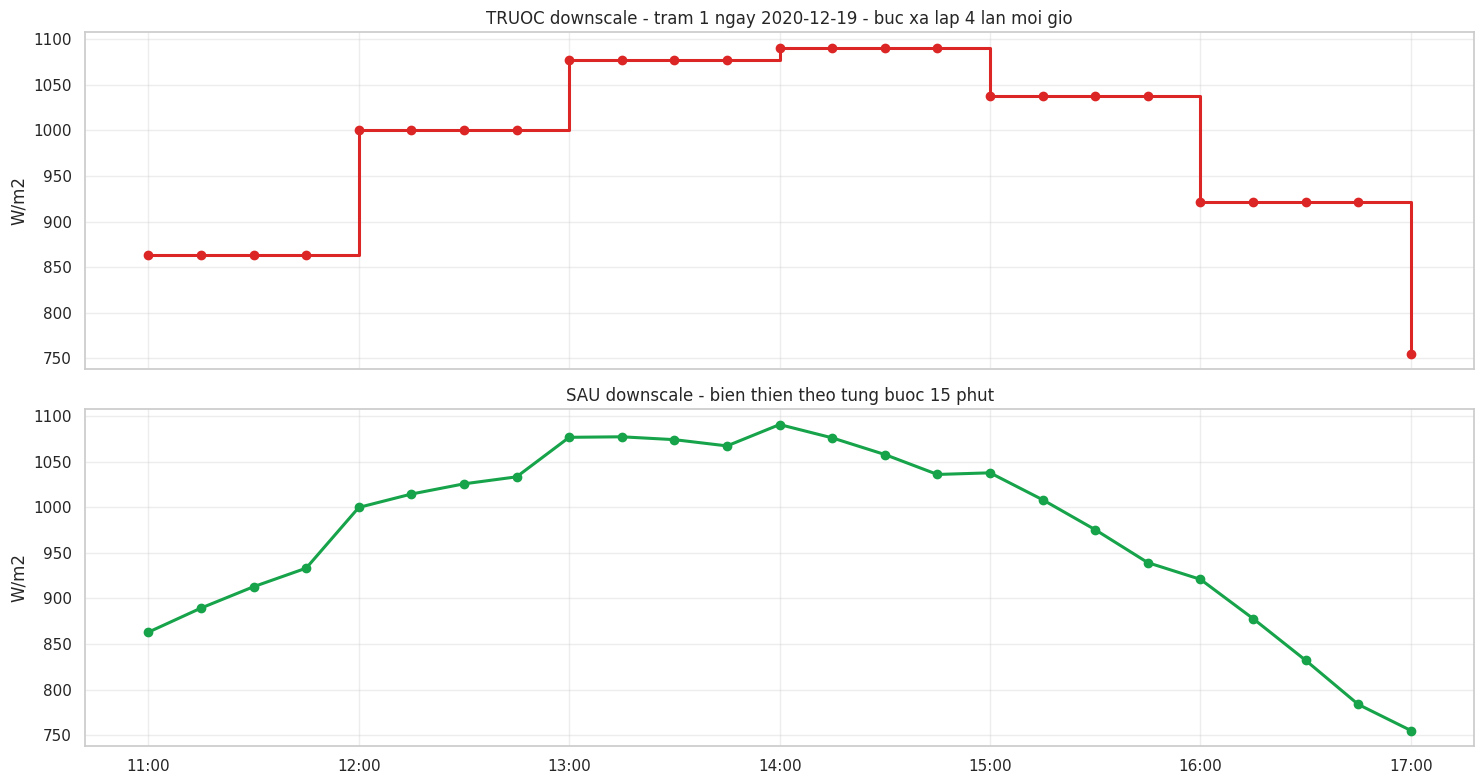
\includegraphics[width=\textwidth]{nb032_downscale_truoc_sau.png}
    
    
    \caption{Làm mịn và nội suy dữ liệu bức xạ bước 15 phút tại trạm 1}
    \label{fig:downscale}
\end{figure}

\subsubsection{Chuẩn hoá quy mô theo trạm}

Bốn mươi hai dàn quang điện có quy mô rất khác nhau, nên quy mô được ước lượng từ chính dữ
liệu và chỉ từ phần huấn luyện: \texttt{site\_scale}, ước lượng chỉ từ phần huấn luyện, là phân vị $99$ của sản lượng ban
ngày, \texttt{tran\_cong\_suat} là phân vị $99{,}9$. Hai mức phân vị này đặt theo quy ước, chưa qua phép quét riêng như cận cắt $k$. Bảng~\ref{tab:quy_mo} trích tám trạm đầu
trong bảng notebook in ra.

\begin{table}[htbp]
\centering
\caption{Quy mô công suất 8 trạm quang điện tiêu biểu}
\label{tab:quy_mo}
\small
\begin{tabular}{r r r r}
\toprule
\textbf{Trạm} & \texttt{site\_scale} & \texttt{tran\_cong\_suat} & \texttt{cs\_factor} \\
\midrule
$27$ & $97{,}19$ & $99{,}00$ & $1{,}55$ \\
$11$ & $92{,}05$ & $92{,}72$ & $1{,}74$ \\
$25$ & $79{,}73$ & $82{,}76$ & $1{,}55$ \\
$18$ & $35{,}05$ & $36{,}35$ & $1{,}56$ \\
$6$  & $27{,}53$ & $28{,}51$ & $1{,}74$ \\
$8$  & $26{,}50$ & $26{,}89$ & $1{,}74$ \\
$1$  & $21{,}50$ & $22{,}81$ & $1{,}70$ \\
$2$  & $18{,}47$ & $19{,}80$ & $1{,}70$ \\
\bottomrule
\end{tabular}


\end{table}

Một mô hình học thẳng trên sản lượng thô sẽ dành phần lớn sức mô tả để phân biệt trạm lớn với trạm nhỏ, thay vì học quan hệ
giữa thời tiết và sản lượng, đó là lý do mục tiêu được chuẩn hoá trước khi huấn luyện.

\subsubsection{Tương tác khí tượng và mã hoá biến phân loại}

Notebook \texttt{03\_3\_features\_aggregate} sinh năm đặc trưng tương tác, xem
Bảng~\ref{tab:tuong_tac}.

\begin{table}[htbp]
\centering
\caption{Tương quan của các đặc trưng tương tác với mục tiêu}
\label{tab:tuong_tac}
\small
% Cot 1 phai du 5,0cm: ten dai nhat la cloud_low_x_shortwave, 21 ky tu chu don cach o
% co \small chiem 4,85cm. De 4,4cm thi no tran khoi cot va dinh lien vao chu cua cot
% "Dinh nghia" ben canh, mat han khoang cach giua hai cot.
\begin{tabular}{@{}L{5.0cm} L{4.6cm} r r@{}}
\toprule
\textbf{Đặc trưng} & \textbf{Định nghĩa} & \textbf{Khuyết} & \textbf{Pearson} \\
\midrule
\texttt{temp\_x\_shortwave} & nhiệt độ $\times$ bức xạ ngang & $0{,}01\%$ & $0{,}3433$ \\
\texttt{diffuse\_ratio} & bức xạ khuếch tán $/$ bức xạ ngang & $47{,}43\%$ & $-0{,}2325$ \\
\texttt{dni\_ratio} & bức xạ trực xạ $/$ bức xạ ngang & $47{,}43\%$ & $0{,}2325$ \\
\texttt{cloud\_x\_shortwave} & mây toàn phần $\times$ bức xạ ngang & $0{,}01\%$ & $0{,}1867$ \\
\texttt{cloud\_low\_x\_shortwave} & mây tầng thấp $\times$ bức xạ ngang & $0{,}01\%$ & $0{,}0945$ \\
\bottomrule
\end{tabular}


\end{table}

Tỷ lệ khuyết $47{,}43\%$ ($735.612$ dòng) của hai đặc trưng dạng thương đến từ mẫu số: ban
đêm bức xạ ngang bằng $0$ nên phép chia không xác định. Giá trị khuyết được giữ nguyên thay
vì điền $0$, để mô hình cây học nhánh riêng cho dữ liệu khuyết. Số giá trị vô cực trên cả
năm cột bằng $0$.

Mã hoá biến phân loại. Bảng mã được khớp chỉ trên phía huấn luyện rồi áp
cho phía kiểm định; notebook khớp được $8$ bảng mã, và số ô gặp hạng mục lạ trên tập kiểm
định bằng $0$.

Kiểm chứng cuối bước sinh đặc trưng. Notebook in ra ba phép kiểm:

% Khoi ket xuat notebook. Khong boc trong minipage nua: minipage la mot hop lien
% khoi, khong the ngat trang, nen khoi dai bi day nguyen sang trang sau va de lai
% khoang trong lon. De verbatim o muc doan van thi no tu ngat duoc.
\begingroup
\par\penalty-150\vspace{8pt}
\small\renewcommand{\baselinestretch}{1.0}\selectfont
\begin{verbatim}
--- KIEM TRA 1: dac trung target deu duoc shift ---
Cot lag con lai sau khi khu tre pha: ['lag_4', 'lag_96']
lag_96(t) == target(t-96) tren mau: DAT
--- KIEM TRA 2: ty le dong co lich su day du ---
- train       : 99.74% dong co du lich su lien tuc
- val         : 100.00% dong co du lich su lien tuc
--- KIEM TRA 3: hang muc la (unseen category) ---
Tong so o gap hang muc la trong val: 0
\end{verbatim}
\par\vspace{8pt}
\endgroup
Sau ba notebook sinh đặc trưng, tập huấn luyện đi từ $48$ cột lên $113$ cột, trong đó $46$
cột là đặc trưng ứng viên; các fold mang $114$ cột do có thêm cột đánh dấu fold.

\FloatBarrier
\subsection{Định nghĩa các đặc trưng dẫn xuất}

Một số cột xuất hiện trong bảng chẩn đoán và bảng chấm điểm ở Mục~\ref{subsec:chan_doan_dac_trung} là đại lượng dẫn xuất,
không đọc thẳng từ dữ liệu nguồn. Bảng~\ref{tab:dinh_nghia_dan_xuat} ghi công thức của chúng.

\begin{table}[htbp]
\centering
\caption{Công thức toán học các đặc trưng dẫn xuất}
\label{tab:dinh_nghia_dan_xuat}
\small
% Cot 2 phai du 7,0cm: o dai nhat la cong thuc clip(shortwave_radiation/ghi_cs, 0, 1,5)
% dat trong \dfrac, khong ngat dong duoc. Bu lai bang cach thu cot 1 (ten cot ngan
% nhat can 3,93cm) va cot 3 (chu tieng Viet, ngat dong duoc). Tong giu nguyen 15,1cm.
\begin{tabular}{@{}L{4.0cm} L{7.0cm} L{4.1cm}@{}}
\toprule
\textbf{Đặc trưng} & \textbf{Công thức} & \textbf{Ý nghĩa} \\
\midrule
\texttt{ky\_vong} &
$\texttt{site\_scale} \times \max(\sin h,\ 0)$ &
Mức sản lượng kỳ vọng của trạm tại góc cao hiện tại, nếu trời hoàn toàn quang \\
\addlinespace
\texttt{ty\_le\_bao\_hoa} &
$\operatorname{clip}\!\left(\dfrac{\texttt{ky\_vong}}{\texttt{tran\_cong\_suat}},\ 0,\ 3\right)$ &
Mức kỳ vọng đã tiến sát trần công suất tới đâu \\
\addlinespace
\texttt{con\_cach\_tran} &
$\texttt{tran\_cong\_suat} - \texttt{ky\_vong}$ &
Khoảng dư còn lại tới trần, tính bằng kWh \\
\addlinespace
\texttt{rad\_x\_sinelev} &
$\texttt{shortwave\_radiation} \times \sin h$ &
Bức xạ chiếu hiệu dụng lên mặt phẳng ngang \\
\addlinespace
\texttt{clearsky\_proxy} &
$(\sin h)^{1{,}2}$ &
Dạng đường cong ngày thuần hình học, nhọn hơn $\sin h$ một chút \\
\addlinespace
\texttt{chi\_so\_troi\_quang} &
$\operatorname{clip}\!\left(\dfrac{\texttt{shortwave\_radiation}}{\texttt{ghi\_cs}},\ 0,\ 1{,}5\right)$ &
Tỷ lệ bức xạ đo được trên bức xạ trời quang đã hiệu chỉnh theo trạm \\
\addlinespace
\texttt{temp\_x\_shortwave} &
$\texttt{temperature\_c} \times \texttt{shortwave\_radiation}$ &
Tương tác nhiệt độ và bức xạ \\
\addlinespace
\texttt{diffuse\_ratio} &
$\operatorname{clip}\!\left(\dfrac{\texttt{diffuse\_solar\_rad.}}{\texttt{shortwave\_rad.}},\ 0,\ 10\right)$ &
Phần khuếch tán chiếm bao nhiêu trong tổng bức xạ \\
\addlinespace
\texttt{cloud\_x\_shortwave} &
$\texttt{cloud\_cover\_total} \times \texttt{shortwave\_radiation}$ &
Tương tác mây toàn phần và bức xạ \\
\bottomrule
\end{tabular}


\end{table}

Về các cột bị loại. Hai cột \texttt{con\_cach\_tran} và \texttt{clearsky\_proxy} được sinh ra ở bước đặc trưng nhưng
không lọt vào bộ được chọn. \texttt{clearsky\_proxy} tương quan $0{,}9973$ với
\texttt{sin\_elevation} nên mang thông tin trùng lặp, còn \texttt{con\_cach\_tran} không đạt ngưỡng
thông tin tương hỗ.

Một đính chính về tên gọi. Tên \texttt{chi\_so\_troi\_quang} gợi ý rằng giá trị $1{,}0$
tương ứng trời hoàn toàn quang. Phép kiểm chứng cho thấy điều đó không đúng với cột này: sau
khi $GHI_{cs}$ đã nhân hệ số hiệu chỉnh theo trạm, tỷ lệ đo được không đạt tới $1{,}0$
ngay cả vào lúc quang nhất giữa trưa, giá trị lớn nhất ở nhóm góc cao $50$--$90^\circ$ chỉ
đạt $0{,}759$. Vì vậy tài liệu này không mô tả nó như một chỉ số trời quang có ý nghĩa vật lý
trực tiếp, mà gọi đúng bản chất là biến tỷ lệ bức xạ đã hiệu chỉnh theo từng trạm. Nó
vẫn hữu ích làm đặc trưng đầu vào vì thứ tự giữa các quan sát trong cùng một trạm được bảo
toàn, mà cây quyết định chỉ dùng thứ tự để tách nhánh.

\textbf{Về cột \texttt{pv\_clr\_lonij}.} Dự án có cài đặt chỉ số $K$ của Lonij đúng nguyên bản
phân vị $80$, cửa sổ trượt $15$ ngày theo từng khung giờ, có \texttt{shift(1)} nên chỉ nhìn quá
khứ thành cột \texttt{pv\_clr\_lonij}. Cột này đạt điểm quan trọng biến $1{,}981$, đứng hạng $6$
trong bảng chẩn đoán ở Mục~\ref{subsec:chan_doan_dac_trung}, nhưng không lọt Top $35$ theo thông tin tương hỗ và không nằm
trong danh sách bảo vệ, nên bị loại ở bước chọn theo đúng quy tắc đã đặt trước.

Cột này nối trực tiếp với lập luận về mức phân vị ở Mục~\ref{subsec:chuan_hoa_muc_tieu}: dự án cài cả phương án phân vị
$80$ của Lonij lẫn phương án phân vị $99$ của mình, rồi để bước chấm điểm quyết định bằng số
liệu thay vì chọn trước bằng lập luận.

\FloatBarrier
\subsection{Thực nghiệm: khử độ trễ cài sẵn bằng đặc trưng tại thời điểm mục tiêu}
\label{subsec:khu_tre_mt}

Vấn đề. Nhãn cần dự báo nằm ở thời điểm $T{+}h$, nhưng các đặc trưng hình học Mặt Trời
và nhãn lịch \texttt{sin\_elevation}, \texttt{ghi\_cs}, \texttt{hour} vẫn là giá trị tại $T$. Mô
hình do đó dùng vị trí Mặt Trời lúc $T$ để dựng lại sản lượng lúc $T{+}h$, và đường dự báo sinh
ra chính là đường Mặt Trời bị trễ đúng $h$ bước. Đây là hệ quả cấu trúc của bài toán, và tác
động của nó lan rộng vì cùng đại lượng đó cũng là mẫu số chuẩn hoá ở Mục~\ref{subsec:chuan_hoa_muc_tieu}.

Cách xử lý. Quy trình khai báo một danh sách $21$ cột tất định hình học
Mặt Trời cùng các đại lượng suy ra từ nó, và toàn bộ nhãn thời gian theo lịch rồi sinh thêm
bản của chúng tại $T{+}h$ với hậu tố \texttt{\_mt}, đồng thời giữ nguyên bản tại $T$. Ở
tầm H1 sinh được $13$ cột, nâng tổng số đặc trưng vào mô hình từ $39$ lên $52$. Nhóm $13$ cột này chỉ gồm vị trí Mặt Trời và nhãn lịch tại $T{+}h$, không chứa sản lượng hay biến khí tượng tại mốc đó.

Ranh giới hợp lệ của phép dịch. Vị trí Mặt Trời và nhãn lịch tại
$T{+}h$ là kết quả tính toán thiên văn và lịch thuần tuý; đứng ở thời điểm $T$ đã biết chính
xác chúng bằng bao nhiêu, không cần chờ tới $T{+}h$ mới đo. Điều này khác hẳn biến khí tượng:
bức xạ và mây tại $T{+}h$ chỉ biết được sau khi đo, nên \texttt{shortwave\_radiation},
\texttt{lag\_96} và toàn bộ nhóm \texttt{rolling\_*} bắt buộc giữ nguyên ở $T$. Ranh giới đó chính là
điều kiện để phép dịch này hợp lệ.

Thêm chứ không thay thế. Quy trình giữ cả bản tại $T$ lẫn bản tại $T{+}h$
của $13$ cột tất định, không thay bản này bằng bản kia.

\FloatBarrier
\subsection{Chuẩn hoá mục tiêu theo vật lý}
\label{subsec:chuan_hoa_muc_tieu}

Bốn mươi trạm có quy mô chênh nhau nhiều lần, và sản lượng trong ngày biến thiên theo góc cao
Mặt Trời. Nếu huấn luyện thẳng trên sản lượng thô, mô hình phải dành phần lớn sức mô tả để
phân biệt trạm lớn với trạm nhỏ và để học lại nhịp ngày đêm, hai thứ đã biết trước bằng
công thức. Mục tiêu vì vậy được đổi sang một tỷ số không thứ nguyên:

\begin{equation}
k_{\text{target}} = \text{clip}\left(\frac{y}{\text{site\_scale} \cdot \max(\sin h, \epsilon)},\, 0,\, k_{\max}\right)
\end{equation}

Mẫu số gồm hai phần: \texttt{site\_scale} khử chênh lệch quy mô giữa các trạm, còn $\sin h$ khử
nhịp ngày đêm. Phép $\max$ đặt một sàn $\varepsilon$ cho mẫu số, vì lúc Mặt Trời sát đường
chân trời thì $\sin h \to 0$ và tỷ số sẽ nổ tung.

Sau khi mô hình dự báo $\hat{k}$, giá trị được nhân ngược về kWh rồi chặn trần:

\begin{equation}
\hat{y} = \min\left(\hat{k} \cdot \text{site\_scale} \cdot \max(\sin h, \epsilon),\, \text{tran\_cong\_suat} \cdot 1{,}02\right)
\end{equation}

Cả \texttt{site\_scale} và \texttt{tran\_cong\_suat} đều là phân vị của chính chuỗi sản lượng nên
mang đơn vị kWh trên mỗi bước $15$ phút, cùng đơn vị với $y$; phép chặn vì vậy không cần hệ số
đổi đơn vị nào.

Cơ sở của cách chuẩn hoá. Việc chia sản lượng đo được cho một mức tham chiếu suy từ
chính hệ thống là cách làm đã có trong tài liệu. Engerer và Mills~\cite{engerer2014kpv} tổng
kết các phương pháp trước đó và dẫn lại chỉ số $K$ của Lonij và cộng sự~\cite{lonij2012tucson},
vốn định nghĩa mức tham chiếu bằng một phân vị của chính sản lượng đo được.

Điểm cần đọc kỹ ở tài liệu nguồn là không có một mức phân vị chuẩn. Ngay trên cùng
một trang tổng kết, hai công trình tiền lệ chọn hai mức khác hẳn nhau. Golnas lấy
phân vị $93$:

\begin{quote}\small
\textit{``After removing days with system outages, the clear-sky BPI (CSBPI) for each system is defined as the 93rd percentile of the set of BPI values in the training set.''}
\end{quote}

Còn Lonij và cộng sự~\cite{lonij2012tucson} lấy phân vị $80$:

\begin{quote}\small
\textit{``$PV_{CLR-L}$ is defined as the 80th percentile of $PV_{MEAS-L}$ at the specified time of day on the previous 15 days for a system.''}
\end{quote}


Hai mức chênh nhau $13$ điểm mà cả hai đều được công bố, vì mỗi bên dựng mẫu số theo một cách.
Điều đó có nghĩa mức phân vị là tham số thiết kế đi kèm cách dựng mẫu số, không phải
hằng số vật lý mượn được từ tài liệu. Mức của dự án vì vậy phải được biện minh bằng thực
nghiệm trên chính dữ liệu của dự án.

Cận cắt suy từ dữ liệu. Tham số $k_{\max}$ không được gán một hằng số
trong tệp cấu hình. Notebook huấn luyện đặt \texttt{CLIP\_K = None} rồi gọi hàm
\texttt{tinh\_clip\_tu\_train()} để tính nó bằng phân vị $99$ của $k$ trên chính tập huấn luyện.
Giá trị thu được và ghi vào \texttt{model\_config.json} là $1{,}3686$, tính trên
$683.715$ giá trị $k$. Mức phân vị $99$ được chọn bằng phép quét ở
Bảng~\ref{tab:quet_phan_vi}.

\begin{table}[htbp]
\centering
\caption{Quét ngưỡng phân vị cận cắt trên tập kiểm định}
\label{tab:quet_phan_vi}
\small
\begin{tabular}{r r r r}
\toprule
\textbf{Mức phân vị} & \textbf{Ngưỡng cắt} & \textbf{Tỷ lệ bị cắt (\%)} & \textbf{WAPE kiểm định (\%)} \\
\midrule
$0{,}900$ & $1{,}1427$ & $10{,}00$ & $22{,}6884$ \\
$0{,}950$ & $1{,}2189$ & $5{,}00$  & $22{,}5407$ \\
$0{,}975$ & $1{,}2888$ & $2{,}50$  & $22{,}5087$ \\
$\mathbf{0{,}990}$ & $\mathbf{1{,}3686}$ & $\mathbf{1{,}00}$ & $\mathbf{22{,}5042}$ \\
$0{,}995$ & $1{,}4291$ & $0{,}50$  & $22{,}5039$ \\
$0{,}999$ & $1{,}5692$ & $0{,}10$  & $22{,}5039$ \\
$1{,}000$ & $6{,}5246$ & $0{,}00$ & $22{,}5039$ \\
\bottomrule
\end{tabular}


\end{table}

Đường cong WAPE phẳng từ mức $0{,}99$ trở lên, ba mức cuối chỉ chênh nhau $0{,}0000$ điểm
phần trăm. Bên dưới mức đó thì sai số xấu dần, tới $22{,}6884\%$ ở phân vị $0{,}90$ vì cắt mất
$10\%$ dữ liệu. Dòng cuối cùng cho thấy phép cắt vẫn cần thiết: bỏ hẳn nó thì ngưỡng nhảy
lên $6{,}5246$, tức đuôi phân bố có những điểm gấp gần năm lần phần thân. Mức $0{,}99$ nằm ở chỗ đường cong bắt đầu phẳng mà vẫn chặn được đuôi đó; các mức từ $0{,}99$
trở lên chênh nhau không đáng kể nên đây là lựa chọn theo quy ước hơn là một điểm tối ưu tách bạch.

Ngưỡng trong bảng và trong cấu hình là một. Phép quét ở Bảng~\ref{tab:quet_phan_vi}
đo WAPE trên tập kiểm định, nhưng ngưỡng cắt của từng mức đều được suy từ phân vị của $k$
trên tập huấn luyện --- đúng nguyên tắc mọi thống kê tham chiếu phải đến từ dữ liệu huấn
luyện. Vì vậy ngưỡng $1{,}3686$ tại mức $0{,}99$ trong bảng trùng khớp với giá trị ghi trong
tệp cấu hình mô hình. Giá trị dùng để huấn luyện và để chấm điểm ở
Mục~\ref{sec:danh_gia_tren_tap_test} là $1{,}3686$.

Ngưỡng cắt của hai tầm và cấu tạo của mẫu số. Bản dựng đầu tiên lấy mẫu số tại
chính thời điểm gốc $T$, còn tử số là sản lượng tại $T+h$. Ở tầm $15$ phút Mặt Trời gần như
đứng yên nên hai vế khớp nhau; ở tầm $60$ phút, buổi sáng Mặt Trời lên nhanh nên mẫu số nhỏ
hơn hẳn tử số và $k$ giàu lên. Vì vậy cùng một quy tắc phân vị $99$ lại cho hai ngưỡng rất
khác nhau: $1{,}3587$ ở tầm H$1$ nhưng $2{,}0039$ ở tầm H$4$. Chênh lệch ấy phản ánh vị trí
Mặt Trời chứ không phản ánh thời tiết.

Cách xử lý. Quy trình chuyển mẫu số sang chính thời điểm cần dự báo, tức lấy
$\sin h$ tại $T+h$ thay cho tại $T$. Việc này không dùng thông tin chưa có: vị trí Mặt Trời
tại $T+h$ tính trước được từ toạ độ trạm và mốc thời gian, cùng lý do cho phép đưa $21$ cột
tất định vào mô hình dưới hậu tố \texttt{\_mt}. Một mẫu số duy nhất được dùng cho cả ba việc:
dựng nhãn $k$, tính trọng số mẫu, và nhân ngược về kWh.

Kết quả. Hai cách dựng mẫu số được so trực tiếp trên cùng dữ liệu, cùng bộ siêu tham
số và cùng tập dòng chấm điểm. Mẫu số tại $T+h$ cho WAPE tốt hơn $0{,}008$ điểm ở tầm H$1$ và
$0{,}237$ điểm ở tầm H$4$ --- khoảng cách nới rộng đúng ở tầm xa, nơi Mặt Trời dịch chuyển
nhiều. Đáng kể hơn con số sai lệch là điều này: phân vị $99$ của $k$ nay bằng nhau ở hai tầm,
cùng bằng $1{,}3686$, nên mỗi tầm suy được ngưỡng từ chính dữ liệu của tầm đó.

Phạm vi đánh giá đi kèm. Vì mẫu số lấy tại $T+h$, điều kiện ban ngày cũng xét tại
$T+h$: một quan sát được đưa vào khi $\sin h$ tại $T+h$ vượt $\varepsilon$. So với cách xét
tại $T$, phạm vi này nhận thêm những mốc thuộc sườn lên buổi sáng và bỏ đi những mốc mà Mặt
Trời đã lặn trước thời điểm cần dự báo. Đây là phạm vi đúng với câu hỏi đặt ra: điều cần biết
là trời có sáng vào lúc được dự báo hay không.

\FloatBarrier
\subsection{Kiểm chứng các tham số cố định}

Các tham số cố định được kiểm chứng trong hai notebook
\texttt{05b\_thuc\_nghiem\_tham\_so} và \texttt{05f\_hop\_le\_hoa\_tham\_so}: sàn mẫu số
$\varepsilon$ được quét trực tiếp (Bảng~\ref{tab:quet_tham_so}), cận cắt qua phép quét mức
phân vị (Bảng~\ref{tab:quet_phan_vi}), hệ số nới trần bằng đo phân bố tỷ lệ sản lượng trên
trần, và chính sách trọng số bằng thực nghiệm bù trừ. Mỗi phép quét chỉ đổi một tham số và giữ nguyên phần còn
lại, rồi huấn luyện và chấm lại trên tập kiểm định. Cách quét từng tham số một không dò được
tương tác giữa chúng, nên kết quả chỉ nói lên độ nhạy của riêng tham số đang xét.

\begin{table}[htbp]
\centering
\caption{Thực nghiệm quét sàn mẫu số $\varepsilon$ trên tập kiểm định}
\label{tab:quet_tham_so}
\small
\begin{tabular}{l r r r r r}
\toprule
\textbf{Tham số} & \textbf{Mức} & \textbf{Dòng huấn luyện} & \textbf{WAPE (\%)} & \textbf{RMSE} & \textbf{$R^2$} \\
\midrule
\texttt{eps\_elev}
 & $0{,}00$ & $604.136$ & $21{,}9892$ & $3{,}6410$ & $0{,}9003$ \\
 & $0{,}02$ & $602.036$ & $21{,}9776$ & $3{,}6365$ & $0{,}9006$ \\
 & $\mathbf{0{,}05}$ & $\mathbf{596.748}$ & $\mathbf{21{,}9627}$ & $\mathbf{3{,}6285}$ & $\mathbf{0{,}9010}$ \\
 & $0{,}10$ & $580.195$ & $21{,}9838$ & $3{,}6337$ & $0{,}9007$ \\
\bottomrule
\end{tabular}


\end{table}

Bảng này phải đọc trung thực, vì không phải tham số nào cũng có tác động như nhau.

Sàn mẫu số $\varepsilon$ ít ảnh hưởng tới độ chính xác. Toàn dải từ $0{,}00$ tới
$0{,}10$ chỉ chênh nhau $0{,}0265$ điểm phần trăm WAPE. Cái mà $\varepsilon$ thực sự điều
khiển là số dòng còn lại để huấn luyện: từ $604.136$ xuống $580.195$, mất $4{,}0\%$. Hai
con số này là hai đầu của dải quét, ứng với $\varepsilon = 0{,}00$ và $\varepsilon = 0{,}10$,
đọc từ ô kết quả notebook \texttt{05b\_thuc\_nghiem\allowbreak \_tham\_so.ipynb} và cột
\texttt{so\_dong\_train} của tệp \texttt{05b\_thuc\_nghiem\_tham\_so/\allowbreak thuc\_nghiem\_tham\_so\_hardcode.csv}.
Mức $0{,}05$ ứng với góc nâng $\arcsin(0{,}05) = 2{,}87^\circ$. Tỷ lệ dòng giữ lại được so với mức
không lọc là

\begin{equation}
\frac{596.748}{604.136} = 0{,}987771 \;\longrightarrow\; \mathbf{98{,}78\%}
\end{equation}

Con số này là tỷ lệ trên các dòng thực sự vào hàm mục tiêu của phép quét ở
Bảng~\ref{tab:quet_tham_so}. Tính trên toàn bộ tập huấn luyện trước khi áp trọng số mẫu thì
tỷ lệ là $683.715 / 714.325 = 95{,}71\%$; hai con số này đọc từ dòng
\texttt{Bi loai khoi ham muc tieu} ở ô kết quả của cùng notebook trên. Hai con số khác nhau vì hai phạm vi khác nhau; báo
cáo dùng $98{,}78\%$ đúng theo phạm vi của bảng.

Phần bị loại nhỏ như vậy vì vành $0 < \sin h \le 0{,}05$ rất hẹp và gần như không phát điện.
Vai trò thật của sàn nằm ở phân bố nhãn: phép quét kèm theo cho thấy nếu hạ sàn xuống
$0{,}005$ thì giá trị $k$ lớn nhất nổ lên $38{,}3$ do phép chia cho mẫu số tiến về $0$, trong
khi ở mức $0{,}05$ chỉ còn $13{,}4$; ngược lại nâng sàn lên $0{,}10$ thì số dòng bị chặn tăng
gần gấp đôi ($8{,}72\%$ so với $4{,}29\%$) mà đuôi phân bố chỉ co thêm không đáng kể (phân vị
$99{,}9$ của $k$ từ $2{,}845$ xuống $2{,}812$). Mức $0{,}05$ vì vậy là điểm cân bằng giữa chặn
vùng chia-cho-số-gần-không và giữ dữ liệu huấn luyện. Mọi con số trong đoạn này đọc từ tệp kết
quả \texttt{05\_selected/\allowbreak quet\_eps\_mau\_chuan\_hoa.csv}.

Cận cắt là tham số có tác động rõ, và được suy từ dữ liệu thay vì gán sẵn. Nó lấy từ
mức phân vị \texttt{clip\_phan\_vi} của tập huấn luyện, và phép quét mức phân vị đã trình bày ở
Bảng~\ref{tab:quet_phan_vi}: hạ mức xuống $0{,}90$ làm WAPE kiểm định xấu đi $0{,}18$ điểm vì
cắt vào phần thân của phân bố; nới lên $1{,}000$ không đổi thêm điểm nào nhưng ngưỡng nhảy lên
$6{,}5246$, tức phép cắt gần như mất tác dụng chặn các điểm đo bất thường. Giá trị áp dụng
là $1{,}3686$ tại mức phân vị $0{,}99$.

Hệ số nới trần được kiểm bằng đo trực tiếp phân bố. Trên $636.138$ dòng đo thật ban
ngày của tập huấn luyện, notebook \texttt{05f\_hop\_le\_hoa\_tham\_so} đo phân bố tỷ lệ (sản
lượng đo được / trần công suất): chỉ $8.285$ dòng ($1{,}3024\%$) vượt mức $1{,}000$, giá trị
lớn nhất đạt $1{,}007$ lần trần, và không dòng nào vượt mức $1{,}020$. Hệ số $1{,}02$ vì vậy
chừa đủ dư địa cho toàn bộ dao động thực tế --- kể cả tăng cường bức xạ ở mép mây --- mà không
thả lỏng thêm, chứ không phải khẳng định công suất lắp đặt thực tế cao hơn $2\%$.

Chính sách trọng số mẫu được chốt bằng thực nghiệm bù trừ. Cơ chế trọng số vùng đỉnh
$w = 1 + k$ của các đợt trước đã được gỡ bỏ, vì trọng số nhìn vào chính nhãn nên gây thiên
lệch dương có hệ thống. Thực nghiệm bù trừ TN11 (tệp
\texttt{05b\_thuc\_nghiem\_tham\_so/\allowbreak tn11\_ablation\_trong\_so.csv}) so ba phương án trên cùng
dữ liệu và cùng cấu hình: giữ $w = 1 + k$ cho WAPE $22{,}7699$ với thiên lệch trung bình
$+0{,}4343$ kWh; tắt trọng số cho $22{,}3182$ và $+0{,}1759$; trọng số tất định $w =$ mẫu số
chuẩn hoá cho kết quả tốt nhất $22{,}1927$ và $+0{,}1164$, đồng thời thẳng hàng với tử số
WAPE vì $\hat{y} - y = \text{mẫu số} \times (\hat{k} - k)$. Cấu hình chính thức dùng
$w =$ mẫu số chuẩn hoá.

Ngưỡng cắt chỉ số trời quang. Tham số \texttt{CLIP\_CSI} chặn tỷ lệ bức xạ đo trên bức xạ
trời quang. Bảng~\ref{tab:clip_csi} cho thấy nó ảnh hưởng tới bao nhiêu điểm bị cắt.

\begin{table}[htbp]
\centering
\caption{Số lượng điểm dữ liệu bị cắt bởi ngưỡng \texttt{CLIP\_CSI}}
\label{tab:clip_csi}
\small
\begin{tabular}{r r r}
\toprule
\textbf{Ngưỡng} & \textbf{Số điểm bị cắt} & \textbf{Tỷ lệ (\%)} \\
\midrule
$1{,}0$ & $39.113$ & $5{,}4447$ \\
$1{,}1$ & $33.082$ & $4{,}6051$ \\
$1{,}2$ & $28.481$ & $3{,}9647$ \\
$1{,}3$ & $24.108$ & $3{,}3559$ \\
$\mathbf{1{,}5}$ & $\mathbf{18.645}$ & $\mathbf{2{,}5955}$ \\
$2{,}0$ & $11.119$ & $1{,}5478$ \\
\bottomrule
\end{tabular}


\end{table}

Ngưỡng $1{,}0$ ứng với giả định bức xạ đo không bao giờ vượt bức xạ trời quang lý thuyết,
giả định đó cắt $5{,}44\%$ số điểm, quá nhiều để coi là hợp lý, vì hiện tượng tăng cường bức
xạ ở mép mây làm bức xạ đo vượt mức trời quang trong thời gian ngắn là có thật. Ngưỡng
$1{,}5$ cắt $2{,}60\%$, giữ lại phần vượt trần do vật lý và chỉ loại phần vượt xa.

\FloatBarrier
\subsection{Chẩn đoán và chọn đặc trưng}
\label{subsec:chan_doan_dac_trung}

Sau ba notebook sinh đặc trưng, tập huấn luyện mang $113$ cột. Hai notebook tiếp theo quyết định
cột nào thực sự đi vào mô hình, với vai trò tách bạch: \texttt{04\_vif\_diagnostics} đo và
xuất bằng chứng, \texttt{05\_select\_features} quyết định. Notebook chẩn đoán không tự loại
cột nào --- nó ghi bảng chỉ số ra tệp để bước chọn đọc lại.

Cách phân vai này có lý do: hệ số phóng đại phương sai chỉ đo mức một đặc trưng bị các đặc trưng
còn lại giải thích, không đo mức đặc trưng đó giải thích được mục tiêu. Một cột có thể vừa cộng
tuyến cao vừa mang thông tin vật lý không thay thế được, nên máy không được quyền tự loại.

\subsubsection{Chẩn đoán đa cộng tuyến}

Trong $113$ cột, $85$ cột được đưa vào chẩn đoán; $28$ cột còn lại nằm ngoài phạm vi vì là mục
tiêu, khoá định danh, cột ghi nguồn gốc dữ liệu, cờ ngoại lai hoặc cột thời gian thô. Kết quả
phân loại trình bày ở Bảng~\ref{tab:chan_doan_nhan}.

\begin{table}[htbp]
\centering
\caption{Phân bố chẩn đoán đa cộng tuyến trên 85 đặc trưng}
\label{tab:chan_doan_nhan}
\small
\begin{tabular}{l r L{7.4cm}}
\toprule
\textbf{Nhãn} & \textbf{Số cột} & \textbf{Nghĩa} \\
\midrule
\texttt{HIGH\_VIF}     & $39$ & Hệ số phóng đại phương sai vượt $10$ \\
\texttt{OK}            & $28$ & Không vướng tiêu chí nào \\
\texttt{CONSTANT}      & $9$  & Chỉ một giá trị duy nhất, phương sai bằng $0$ \\
\texttt{DUPLICATE}     & $8$  & Trùng lặp gần hoàn hảo với một cột khác \\
\texttt{HIGH\_MISSING} & $1$  & Tỷ lệ khuyết quá cao \\
\midrule
\textbf{Tổng} & $\mathbf{85}$ & \\
\bottomrule
\end{tabular}


\end{table}

Cột duy nhất mang nhãn khuyết cao là \texttt{source\_gap\_id} với $97{,}68\%$ ô trống đúng bản
chất của nó, vì nó chỉ nhận giá trị tại các dòng nằm trong một khoảng trống nguồn.

Cột trùng lặp. Ở ngưỡng $|r| \ge 0{,}95$ notebook đếm được $43$ cặp, nhưng chỉ những
cặp đạt $|r| \ge 0{,}9999$ mới bị coi là trùng lặp thực sự, vì cộng tuyến hoàn hảo khiến phép
tính hệ số phóng đại phương sai không xác định. Tám cột bị loại ở bước này, xem
Bảng~\ref{tab:trung_lap}.

\begin{table}[htbp]
\centering
\caption{Các cặp đặc trưng trùng lặp và cột đại diện giữ lại}
\label{tab:trung_lap}
% \footnotesize thay vi \small: bang nay de cot tu gian, ma hai ten dai nhat
% (number_of_panels_missing_flag va capacity_kw_missing_flag) cong lai vuot kho chu
% 23,65pt. Ten cot la du lieu that, khong duoc rut gon, nen ha co chu.
\footnotesize
\begin{tabular}{l l r}
\toprule
\textbf{Cột bị bỏ} & \textbf{Đại diện giữ lại} & \textbf{Số giá trị phân biệt} \\
\midrule
\texttt{quarter\_hour}                  & \texttt{minute\_of\_day}            & $96$ \\
\texttt{hour\_of\_day}                  & \texttt{hour}                       & $24$ \\
\texttt{hour\_bucket\_raw}              & \texttt{hour}                       & $24$ \\
\texttt{hour\_bucket\_model}            & \texttt{hour}                       & $24$ \\
\texttt{day\_of\_week\_model}           & \texttt{day\_of\_week}              & $7$ \\
\texttt{month\_model}                   & \texttt{month}                      & $12$ \\
\texttt{number\_of\_panels\_missing\_flag} & \texttt{capacity\_kw\_missing\_flag} & $2$ \\
\texttt{dni\_ratio}                     & \texttt{diffuse\_ratio}             & $37.341$ \\
\bottomrule
\end{tabular}


\end{table}

Sáu nhóm đầu là các cách mã hoá khác nhau của cùng một đại lượng thời gian, sinh ra ở các bước
khác nhau của quy trình rồi cùng tồn tại. Cặp \texttt{diffuse\_ratio} và \texttt{dni\_ratio} có
$r = -1{,}0000$ vì hai tỷ lệ này cộng lại bằng $1$ theo định nghĩa. Sau bước loại trùng, số đặc
trưng còn $77$.

Hệ số phóng đại phương sai. Bảng~\ref{tab:vif} lấy tám cột cao nhất.

\begin{table}[htbp]
\centering
\caption{Tám đặc trưng có hệ số phóng đại phương sai (VIF) cao nhất}
\label{tab:vif}
\small
\begin{tabular}{l r L{6.6cm}}
\toprule
\textbf{Đặc trưng} & \textbf{VIF} & \textbf{Nguồn cộng tuyến} \\
\midrule
\texttt{direct\_normal\_irradiance} & $9999$   & Ba cột bức xạ ràng buộc nhau qua quan hệ hình học \\
\texttt{diffuse\_solar\_radiation}  & $9999$   & \\
\texttt{shortwave\_radiation}      & $9999$   & \\
\texttt{tran\_cong\_suat}           & $6.505{,}32$ & Cùng suy từ phân vị sản lượng của một trạm \\
\texttt{site\_scale}               & $6.381{,}60$ & \\
\texttt{month}                    & $5.170{,}17$ & Trùng thông tin với biến ngày trong năm \\
\texttt{day\_of\_year}              & $5.160{,}63$ & \\
\texttt{sin\_elevation}            & $2.042{,}02$ & Hàm xác định của cùng góc cao Mặt Trời \\
\bottomrule
\end{tabular}


\end{table}

Ba cột bức xạ đạt mức chặn trên vì $GHI$ bằng tổng của thành phần trực xạ chiếu xuống mặt ngang
và thành phần khuếch tán, nên biết hai cột là suy ra được cột còn lại. Cặp \texttt{site\_scale} và
\texttt{tran\_cong\_suat} có $r = 0{,}9998$ vì cả hai là phân vị $99$ và phân vị $99{,}9$ của cùng
một chuỗi sản lượng.

Không cột nào trong Bảng~\ref{tab:vif} bị loại. Cộng tuyến làm hệ số của mô hình tuyến tính mất
ổn định, nhưng mô hình dùng ở đây là cây quyết định tăng cường gradient nó chọn điểm cắt
theo mức giảm hàm mất mát chứ không giải hệ phương trình chuẩn tắc, nên không chịu ảnh hưởng đó.

Đối chiếu bằng một phương pháp độc lập. Để không quyết định chỉ dựa trên một thước đo,
notebook chạy thêm hồi quy bình phương tối thiểu riêng phần và lấy điểm quan trọng biến, đo theo
hiệp phương sai với mục tiêu thay vì theo cộng tuyến giữa các đặc trưng. Bảy đặc trưng đứng đầu
được ghi ở Bảng~\ref{tab:pls}.

\begin{table}[htbp]
\centering
\caption{Đặc trưng dẫn đầu theo độ quan trọng PLS và hệ số VIF tương ứng}
\label{tab:pls}
\small
\begin{tabular}{l r r}
\toprule
\textbf{Đặc trưng} & \textbf{Điểm quan trọng} & \textbf{VIF} \\
\midrule
\texttt{rolling\_mean\_4} & $2{,}283$ & $467{,}40$ \\
\texttt{rolling\_min\_4}  & $2{,}266$ & $873{,}04$ \\
\texttt{rolling\_max\_4}  & $2{,}245$ & $1.412{,}58$ \\
\texttt{lag\_4}          & $2{,}145$ & $28{,}26$ \\
\texttt{ky\_vong}        & $2{,}062$ & $21{,}58$ \\
\texttt{pv\_clr\_lonij}   & $1{,}981$ & $10{,}55$ \\
\texttt{lag\_96}         & $1{,}907$ & $5{,}46$ \\
\bottomrule
\end{tabular}


\end{table}

Sáu trong bảy đặc trưng dẫn đầu đồng thời mang nhãn cộng tuyến cao. Đây là lý do trực tiếp để
bước chọn không dùng hệ số phóng đại phương sai làm tiêu chí loại: nếu cắt theo ngưỡng $10$ thì
sáu đặc trưng mạnh nhất theo thước đo độc lập sẽ bị loại hết.

\subsubsection{Danh sách cấm}

Trước khi chấm điểm, notebook \texttt{05\_select\_features} khai báo tường minh một danh sách cấm
gồm $54$ tên cột. Danh sách này chặn bốn loại: chính mục tiêu và các biến thể của nó, cờ ngoại
lai và cột loại trừ huấn luyện, cột ghi nguồn gốc dữ liệu, và các khoá định danh cùng cột thời
gian thô.

Danh sách được khai báo theo tên chứ không theo tập dữ liệu, nên nó bao cả những tên chỉ xuất
hiện ở các bước khác của quy trình. Trong $113$ cột của tệp đầu vào, $39$ cột trùng tên với
danh sách và bị loại; $74$ cột còn lại đi tiếp vào bước chấm điểm. Cách khai báo dư này là có
chủ đích: thêm một tên không tồn tại thì vô hại, còn sót một tên rò rỉ thì hỏng cả kết quả.

Danh sách cấm được đặt trước phép chấm điểm chứ không sau, vì một cột rò rỉ luôn đạt điểm tương quan cao: nếu để cột đó tham gia đánh giá thì chính thước đo sẽ chọn nhầm đặc trưng rò rỉ thông tin tương lai.

\subsubsection{Chấm điểm bằng thông tin tương hỗ}

Phép chấm điểm chạy trên thông tin tương hỗ giữa từng đặc trưng và mục tiêu. Thước đo
này bắt được cả quan hệ phi tuyến, khác hệ số tương quan Pearson vốn chỉ đo quan hệ tuyến
tính~--- điều cần thiết ở đây vì quan hệ giữa bức xạ và sản lượng bão hoà dần khi tới gần trần công
suất.

Điểm chỉ tính trên các dòng hợp lệ, tức đã bỏ dòng mang cờ loại trừ huấn luyện:

% Khoi ket xuat notebook. Khong boc trong minipage nua: minipage la mot hop lien
% khoi, khong the ngat trang, nen khoi dai bi day nguyen sang trang sau va de lai
% khoang trong lon. De verbatim o muc doan van thi no tu ngat duoc.
\begingroup
\par\vspace{6pt}\hrule\vspace{4pt}
\small\renewcommand{\baselinestretch}{1.0}\selectfont
\begin{verbatim}
Dich muc tieu sang T+1 buoc: bo 42 dong cuoi moi tram
Tổng số dòng ban đầu: 1550856
Số dòng hợp lệ (exclude_from_training == False): 1520073 (98.02%)
Số dòng bị loại trừ khỏi chấm điểm: 30783
\end{verbatim}
\vspace{2pt}\hrule\par\vspace{6pt}
\endgroup

Bảng~\ref{tab:mi} lấy mười đặc trưng đứng đầu trong $74$ ứng viên, chấm trên mẫu $100.000$ dòng.

\begin{table}[htbp]
\centering
\caption{Mười đặc trưng có điểm thông tin tương hỗ (MI) cao nhất}
\label{tab:mi}
\small
\begin{tabular}{r l r}
\toprule
\textbf{Hạng} & \textbf{Đặc trưng} & \textbf{Điểm} \\
\midrule
$1$  & \texttt{ky\_vong}         & $1{,}0778$ \\
$2$  & \texttt{rolling\_max\_4}   & $0{,}9733$ \\
$3$  & \texttt{rolling\_mean\_4}  & $0{,}9513$ \\
$4$  & \texttt{rolling\_min\_4}   & $0{,}9183$ \\
$5$  & \texttt{lag\_96}          & $0{,}9100$ \\
$6$  & \texttt{solar\_elevation} & $0{,}8268$ \\
$7$  & \texttt{ghi\_cs}          & $0{,}8038$ \\
$8$  & \texttt{ty\_le\_bao\_hoa}   & $0{,}7998$ \\
$9$  & \texttt{sin\_elevation}   & $0{,}7989$ \\
$10$ & \texttt{rad\_x\_sinelev}   & $0{,}7415$ \\
\bottomrule
\end{tabular}


\end{table}

Đứng đầu là \texttt{ky\_vong} --- tích của quy mô trạm với $\sin$ góc cao Mặt Trời, tức mức
sản lượng kỳ vọng theo hình học. Ba vị trí kế tiếp là thống kê cửa sổ trượt một giờ và vị trí
thứ năm là giá trị cùng khung giờ ngày hôm trước, đều suy từ lịch sử của chính chuỗi sản lượng. Bảng xếp hạng này khớp với kết quả tự tương quan ở Mục~\ref{subsec:kham_pha_du_lieu}: chuỗi mang
tự tương quan $+0{,}9035$ tại mốc một giờ, nên các thống kê của cửa sổ một giờ gần nhất là nguồn
thông tin mạnh nhất về giá trị sắp tới.

\subsubsection{Danh sách bảo vệ}

Lấy thẳng $35$ đặc trưng đứng đầu sẽ loại mất một số biến khí tượng và hình học Mặt Trời có điểm
thấp nhưng cần cho mô hình đọc được điều kiện vật lý tại bước hiện tại. Notebook vì vậy khai báo
một danh sách bảo vệ gồm $21$ đặc trưng, cả $21$ đều có mặt trong dữ liệu, và bổ sung lại những
đặc trưng nằm ngoài ngưỡng cắt:

% Khoi ket xuat notebook. Khong boc trong minipage nua: minipage la mot hop lien
% khoi, khong the ngat trang, nen khoi dai bi day nguyen sang trang sau va de lai
% khoang trong lon. De verbatim o muc doan van thi no tu ngat duoc.
\begingroup
\par\vspace{6pt}\hrule\vspace{4pt}
\footnotesize\renewcommand{\baselinestretch}{1.0}\selectfont
\begin{verbatim}
--- DANH SACH BAO VE ---
Co trong du lieu   : 21/21
Bi Top K cat, da bo sung lai (4): ['azimuth_sin', 'temperature_c',
                                   'doy_sin', 'doy_cos']
Tong dac trung duoc chon: 35 (Top K) + 4 (bao ve) = 39
\end{verbatim}
\vspace{2pt}\hrule\par\vspace{6pt}
\endgroup

Bốn đặc trưng được bổ sung lần lượt đứng hạng $39$ (\texttt{azimuth\_sin}), $40$
(\texttt{temperature\_c}), $49$ (\texttt{doy\_cos}) và $56$ (\texttt{doy\_sin}) theo điểm thông tin tương
hỗ. Hai cột \texttt{doy\_sin} và \texttt{doy\_cos} mã hoá vị trí trong năm dưới dạng vòng; điểm của
chúng thấp vì trên một mẫu ngẫu nhiên rải khắp $18$ tháng, mùa gần như không phân biệt được 
nhưng mô hình cần chúng để không coi ngày $31/12$ và ngày $01/01$ là hai thời điểm xa nhau.

\subsubsection{Kết quả áp cho mười tập}

Ba mươi chín đặc trưng cơ bản đã chọn~--- mở rộng thành $52$ ở cả hai tầm sau khi thêm $13$ cột thiên văn và lịch tính sẵn tại $T{+}h$~--- được áp đồng loạt cho mười tập dữ liệu bốn tập chính và sáu phần
của ba fold:

% Khoi ket xuat notebook. Khong boc trong minipage nua: minipage la mot hop lien
% khoi, khong the ngat trang, nen khoi dai bi day nguyen sang trang sau va de lai
% khoang trong lon. De verbatim o muc doan van thi no tu ngat duoc.
\begingroup
\par\vspace{6pt}\hrule\vspace{4pt}
\small\renewcommand{\baselinestretch}{1.0}\selectfont
\begin{verbatim}
--- DA LOC 10 TAP THEO 39 DAC TRUNG DA CHON ---
              tap     dong  cot_truoc  cot_sau  feature  cot_phu  \
0        v5_train  1550856        113       49       39       10   
1          v5_val   723114        113       49       39       10   
2         v5_test   510468        113       49       39       10   
3  v5_development  2273970        112       49       39       10   
4    fold_1_train   233244        114       49       39       10   
5      fold_1_val   606105        114       49       39       10   
6    fold_2_train   839349        114       49       39       10   
7      fold_2_val   711507        114       49       39       10   
8    fold_3_train  1550856        114       49       39       10   
9      fold_3_val   723114        114       49       39       10   

   feature_thieu  
0              0  
1              0  
2              0  
3              0  
4              0  
5              0  
6              0  
7              0  
8              0  
9              0  

Moi tap deu co du dac trung da chon.
\end{verbatim}
\vspace{2pt}\hrule\par\vspace{6pt}
\endgroup

Cột \texttt{feature\_thieu} bằng $0$ ở cả mười dòng, tức không tập nào thiếu đặc trưng đã chọn.
Mỗi tập giữ $49$ cột: $39$ đặc trưng cùng $10$ cột phụ trợ gồm mục tiêu, mốc thời gian, mã trạm
và các cột phục vụ lọc phạm vi chấm điểm. Danh sách $39$ tên cột được ghi ra tệp
\texttt{selected\_features.json} để các bước huấn luyện và phục vụ đọc lại đúng một danh sách duy
nhất.

\FloatBarrier
\subsection{Tổng hợp bộ đặc trưng đưa vào mô hình}

Bảng~\ref{tab:bo_dac_trung} tổng hợp toàn bộ $39$ đặc trưng cơ bản được lựa chọn (mở rộng thành $52$ đặc trưng sau khi thêm các biến mục tiêu tương lai $T+h$ cho H1) đưa vào huấn luyện mô hình, phân loại theo 6 nhóm chức năng.

\begin{table}[htbp]
\centering
\caption{Danh mục $39$ đặc trưng cơ bản chọn ở bước $05$, trước khi thêm $13$ cột tại $T{+}h$}
\label{tab:bo_dac_trung}
\footnotesize
\renewcommand{\arraystretch}{1.08}
\begin{tabularx}{\textwidth}{@{} >{\raggedright\arraybackslash}p{3.8cm} c >{\raggedright\arraybackslash}X @{}}
\toprule
\textbf{Nhóm Đặc Trưng} & \textbf{Số Cột} & \textbf{Danh Sách Tên Cột} \\
\midrule
Thời gian và lịch tuần hoàn & $5$ &
\texttt{minute\_of\_day}, \texttt{hour}, \texttt{hour\_cos}, \texttt{doy\_sin}, \texttt{doy\_cos} \\
\addlinespace[3pt]
Solar geometry và trời quang & $8$ &
\texttt{solar\_elevation}, \texttt{sin\_elevation}, \texttt{solar\_azimuth}, \texttt{azimuth\_sin}, \texttt{azimuth\_cos}, \texttt{ghi\_cs}, \texttt{cs\_factor}, \texttt{chi\_so\_troi\_quang} \\
\addlinespace[3pt]
Khí tượng quan trắc & $4$ &
\texttt{shortwave\_radiation}, \texttt{diffuse\_solar\_radiation}, \texttt{direct\_normal\_irradiance}, \texttt{temperature\_c} \\
\addlinespace[3pt]
Tương tác vật lý và tỷ lệ & $5$ &
\texttt{rad\_x\_sinelev}, \texttt{temp\_x\_shortwave}, \texttt{diffuse\_ratio}, \texttt{cloud\_x\_shortwave}, \texttt{cloud\_low\_x\_shortwave} \\
\addlinespace[3pt]
Lịch sử chuỗi thời gian & $9$ &
\texttt{lag\_4}, \texttt{lag\_96}, \texttt{rolling\_mean\_4}, \texttt{rolling\_std\_4}, \texttt{rolling\_min\_4}, \texttt{rolling\_max\_4}, \texttt{rolling\_mean\_96}, \texttt{rolling\_std\_96}, \texttt{rolling\_max\_96} \\
\addlinespace[3pt]
Quy mô trạm và mã hoá & $8$ &
\texttt{ky\_vong}, \texttt{ty\_le\_bao\_hoa}, \texttt{tran\_cong\_suat}, \texttt{capacity\_kw}, \texttt{site\_id\_enc}, \texttt{inverter\_enc}, \texttt{weather\_condition\_enc}, \texttt{weather\_description\_enc} \\
\midrule
\textbf{Tổng số đặc trưng} & $\mathbf{39}$ & \\
\bottomrule
\end{tabularx}


\end{table}

% Khoi verbatim ben duoi cong hai dong ket luan vua qua chieu cao trang, de lai mot
% trang gan nhu trong. Noi trang nay them ba dong de hai dong do khong bi day sang.
\enlargethispage{3\baselineskip}
Mười ba cột \texttt{\_mt} sinh thêm ở bước huấn luyện đều thuộc hai nhóm đầu hình học Mặt Trời
và nhãn lịch đúng theo ranh giới hợp lệ đã nêu ở Mục~\ref{subsec:khu_tre_mt}:

% Khoi ket xuat notebook. Khong boc trong minipage nua: minipage la mot hop lien
% khoi, khong the ngat trang, nen khoi dai bi day nguyen sang trang sau va de lai
% khoang trong lon. De verbatim o muc doan van thi no tu ngat duoc.
\begingroup
\par\penalty-150\vspace{8pt}
\small\renewcommand{\baselinestretch}{1.0}\selectfont
\begin{verbatim}
Them 13 dac trung tat dinh tai T+15 phut:
   ['solar_elevation_mt', 'solar_azimuth_mt', 'azimuth_sin_mt',
    'azimuth_cos_mt', 'sin_elevation_mt', 'ghi_cs_mt', 'ky_vong_mt',
    'ty_le_bao_hoa_mt', 'minute_of_day_mt', 'hour_mt',
    'hour_cos_mt', 'doy_sin_mt', 'doy_cos_mt']
Ma tran train : 596,748 dong x 52 dac trung
Muc tieu chuan hoa k: min 0.0028  trung vi 0.6490  max 1.3686
\end{verbatim}
\par\vspace{8pt}
\endgroup
Không cột khí tượng nào có mặt trong danh sách này. Giá trị lớn nhất của mục tiêu chuẩn hoá
bằng đúng $1{,}3686$, tức cận cắt suy từ phân vị $99$ ở Mục~\ref{subsec:chuan_hoa_muc_tieu} đang hoạt động.
\newpage
\FloatBarrier
\section{Huấn luyện và chọn hàm mất mát}

Mô hình là LightGBM hồi quy, huấn luyện riêng cho H1 và H4, mỗi tầm nhận $52$ đặc trưng.
Mục này đi qua năm bước: trọng số cho dòng ngoại lai, tinh chỉnh siêu tham số
(\textit{hyperparameter}), sáu cấu hình chọn được, chọn hàm mất mát, và cấu hình tất định.

\FloatBarrier
\subsection{Chính sách trọng số cho dòng ngoại lai}

Các dòng mang nhãn ngoại lai không bị xoá khỏi lưới. Chúng nhận trọng số bằng $0$, tức không
đóng góp vào hàm mục tiêu, nhưng vẫn nằm trong bảng để bước báo cáo truy ngược được:

% Khoi ket xuat notebook. Khong boc trong minipage nua: minipage la mot hop lien
% khoi, khong the ngat trang, nen khoi dai bi day nguyen sang trang sau va de lai
% khoang trong lon. De verbatim o muc doan van thi no tu ngat duoc.
\begingroup
\par\penalty-150\vspace{8pt}
\footnotesize\renewcommand{\baselinestretch}{1.0}\selectfont
\begin{verbatim}
--- CHINH SACH OUTLIER, experiment = measured_only_headline ---
Dong co weight = 0 khong tham gia ham muc tieu nhung van giu de bao cao.
Tong dong bi loai khoi ham muc tieu: 86,967 / 683,715 (12.72%)
   trong do physical_over_capacity: 0 dong (luon bi loai o moi experiment)
Khoang thoi gian train: 2020-01-02 06:15:00 -> 2021-06-21 16:45:00
\end{verbatim}
\par\vspace{8pt}
\endgroup
Cách gán trọng số $0$ được chọn thay vì xoá dòng, vì xoá sẽ làm đứt lưới thời gian và mọi đặc
trưng trễ, cửa sổ trượt tính sau đó đều đếm sai khoảng cách, đúng vấn đề mà bước dựng lưới ở
Mục~\ref{subsec:hien_trang_du_lieu} đặt ra để tránh.

\FloatBarrier
\subsection{Tinh chỉnh siêu tham số (\textit{hyperparameter})}

Mỗi hàm mất mát được Optuna chạy một phiên tìm kiếm riêng với ngân sách $20$ trial,
chấm bằng WAPE gộp trên ba fold cửa sổ mở rộng của tập Phát triển. Không hàm nào phải dùng lại
bộ tham số của hàm khác, và không hàm nào bị cố định mức điều hoà.

Miền tìm kiếm khai báo cố định trong cả ba notebook huấn luyện, ghi ở
Bảng~\ref{tab:mien_optuna}.

\begin{table}[htbp]
\centering
\caption{Không gian tìm kiếm siêu tham số cho Optuna}
\label{tab:mien_optuna}
\small
\begin{tabular}{l l l}
\toprule
\textbf{Siêu tham số} & \textbf{Miền} & \textbf{Vai trò} \\
\midrule
\texttt{n\_estimators}     & $[400;\ 1200]$ & Số cây tối đa, early stopping chốt số thật \\
\texttt{learning\_rate}    & $[0{,}02;\ 0{,}12]$ thang log & Tốc độ học \\
\texttt{num\_leaves}       & $[63;\ 255]$ & Độ phức tạp mỗi cây \\
\texttt{min\_child\_samples} & $[20;\ 120]$ & Số mẫu tối thiểu mỗi lá \\
\texttt{subsample}         & $[0{,}7;\ 1{,}0]$ & Tỷ lệ mẫu mỗi vòng \\
\texttt{colsample\_bytree} & $[0{,}7;\ 1{,}0]$ & Tỷ lệ cột mỗi cây \\
\texttt{reg\_alpha}        & $[0;\ 10]$ & Điều hoà $L_1$ \\
\texttt{reg\_lambda}       & $[0;\ 10]$ & Điều hoà $L_2$ \\
\texttt{alpha}             & $[0{,}05;\ 0{,}5]$ thang log & Điểm chuyển của Huber, chỉ Huber có \\
\bottomrule
\end{tabular}


\end{table}

Vì \texttt{reg\_alpha} và \texttt{reg\_lambda} được thả độc lập trên cùng một miền, không gian
tìm kiếm bao trùm cả ba chế độ điều hoà: $L_1$ thuần, $L_2$ thuần và dạng phối hợp. Mỗi hàm mất
mát vì vậy được trao cơ hội ngang nhau để tự tìm mức điều hoà phù hợp trước khi đem ra so.

\FloatBarrier
\subsection{Sáu cấu hình Optuna chọn được}

\begin{table}[htbp]
\centering
\caption{Bộ siêu tham số Optuna chọn được trong miền tìm kiếm, theo từng cấu hình}
\label{tab:sieu_tham_so}
\scriptsize
\resizebox{\textwidth}{!}{\begin{tabular}{l r r r r r r r r}
\toprule
\textbf{Cấu hình} & \textbf{Số cây} & \textbf{Tốc độ học} & \textbf{Số lá} &
\textbf{Mẫu/lá} & \textbf{Tỷ lệ mẫu} & \textbf{Tỷ lệ cột} & $\boldsymbol{L_1}$ & $\boldsymbol{L_2}$ \\
\midrule
\textbf{MAE --- H1}  & $450$ & $0{,}05375$ & $64$  & $116$ & $0{,}970$ & $0{,}838$ & $1{,}82$ & $6{,}02$ \\
Huber --- H1         & $929$ & $0{,}04376$ & $80$ & $49$ & $0{,}707$ & $0{,}862$ & $5{,}00$ & $2{,}51$ \\
MSE --- H1           & $388$ & $0{,}05812$ & $86$ & $67$ & $0{,}773$ & $0{,}948$ & $0{,}06$ & $2{,}67$ \\
\addlinespace
\textbf{MAE --- H4}  & $200$ & $0{,}03695$ & $124$  & $88$ & $0{,}742$ & $0{,}875$ & $4{,}92$ & $2{,}69$ \\
Huber --- H4         & $899$ & $0{,}03618$ & $75$ & $51$ & $0{,}798$ & $0{,}919$ & $6{,}38$ & $8{,}87$ \\
MSE --- H4           & $969$ & $0{,}03412$ & $252$ & $88$ & $0{,}717$ & $0{,}998$ & $5{,}31$ & $6{,}98$ \\
\bottomrule
\end{tabular}}


\end{table}

Điểm chuyển của Huber không còn được thả tự do trên một dải rộng: notebook suy nó từ chính
phần dư của một lần khớp sơ bộ ngoài mẫu --- ước lượng độ lệch chuẩn vững
$\sigma = 1{,}4826 \times \mathrm{MAD} = 0{,}1267$ rồi lấy $\delta = 1{,}345\sigma = 0{,}1704$
theo quy tắc Huber (1964), tương ứng $27{,}67\%$ số dòng rơi vào vùng tuyến tính --- và miền
tìm kiếm $[0{,}05;\ 0{,}5]$ đặt quanh giá trị đó. Optuna chốt $\alpha = 0{,}1712$ ở H1 và
$0{,}1483$ ở H4, đều nằm gọn giữa miền chứ không dạt về biên. Đọc ngang bảng còn thấy số cây
thực dùng không đi theo một chiều: MSE cần nhiều cây hơn hẳn ở tầm xa ($969$ so với $388$),
Huber gần như không đổi ($899$ so với $929$), còn MAE lại dừng sớm hơn ($200$ so với $450$) ---
mỗi hàm mất mát hấp thụ độ khó của tầm xa theo một cách riêng.

Chỗ chạm biên miền tìm kiếm. Năm siêu tham số (\textit{hyperparameter}) dừng sát
biên: \texttt{num\_leaves} của MAE--H1 bằng $64$ và của MSE--H4 bằng $252$ trên miền
$[63;\ 255]$, \texttt{subsample} của Huber--H1 bằng $0{,}707$, \texttt{reg\_alpha} của MSE--H1
bằng $0{,}064$, \texttt{colsample\_bytree} của MSE--H4 bằng $0{,}998$. Khi một siêu tham số
dừng ngay tại biên, không thể loại trừ khả năng giá trị tốt hơn nằm ngoài miền đã khai báo,
nên tài liệu này chỉ tuyên bố đây là cấu hình tốt nhất tìm được trong miền và ngân sách $20$
trial đã khoá từ trước. Ba chỗ dạt cận dưới đều theo hướng ít điều chỉnh hơn, phù hợp với mục
tiêu chuẩn hoá đã mượt hơn sau khi bỏ thừa số hình học.

\FloatBarrier
\subsection{Chọn hàm mất mát}
\label{subsec:chon_ham_mat_mat}

Ba hàm được chấm trên tập kiểm định, phần dữ liệu mô hình chưa từng nhìn thấy, ở phạm vi
đo thật ban ngày. Phạm vi này xét dòng nhãn tại $T{+}h$ đúng như ở bước đánh giá cuối
tại Mục~\ref{subsec:pham_vi_cham_diem}, và loại hai trạm $19$, $24$ cho khớp với phạm vi huấn luyện. Kết quả đầy đủ của
sáu cấu hình ở Bảng~\ref{tab:chon_loss}.

\begin{table}[htbp]
\centering
\caption{Sai số trên tập kiểm định theo các hàm mất mát}
\label{tab:chon_loss}
\small
\begin{tabular}{l l r r r r}
\toprule
\textbf{Tầm} & \textbf{Hàm mất mát} & \textbf{WAPE (\%)} & \textbf{RMSE} & \textbf{MAE} & \textbf{$R^2$} \\
\midrule
\multicolumn{6}{@{}l}{\textit{H1 --- $288.216$ quan sát cho cả ba hàm}} \\
H1 & \textbf{MAE}  & $\mathbf{21{,}8684}$ & $3{,}6201$ & $1{,}4967$ & $0{,}9015$ \\
H1 & MSE           & $22{,}4822$ & $3{,}6116$ & $1{,}5387$ & $0{,}9019$ \\
H1 & Huber         & $22{,}1592$ & $3{,}6099$ & $1{,}5166$ & $0{,}9020$ \\
\addlinespace
\multicolumn{6}{@{}l}{\textit{H4 --- $288.216$ quan sát cho cả ba hàm}} \\
H4 & \textbf{MAE}  & $\mathbf{25{,}8240}$ & $4{,}1088$ & $1{,}7674$ & $0{,}8731$ \\
H4 & MSE           & $26{,}5108$ & $4{,}1439$ & $1{,}8144$ & $0{,}8709$ \\
H4 & Huber         & $25{,}9443$ & $4{,}0965$ & $1{,}7756$ & $0{,}8738$ \\
\bottomrule
\end{tabular}


\end{table}

MAE cho sai số thấp nhất ở cả hai tầm và được chọn cho cả hai. Trong mỗi tầm, ba hàm
được chấm trên đúng cùng số quan sát, điều kiện để phép so sánh có nghĩa, vì nếu một cấu
hình được chấm trên tập sạch hơn thì chênh lệch WAPE phản ánh phạm vi chứ không phản ánh hàm
mất mát.

Đáng chú ý là thứ hạng đổi theo thước đo. Trên WAPE, MAE đứng đầu ở cả hai tầm. Trên RMSE,
Huber mới là hàm thấp nhất, cũng ở cả hai tầm ($3{,}6099$ và $4{,}0965$); MAE tụt xuống cuối ở
H1 ($3{,}6201$) nhưng vẫn đứng trên MSE ở H4 ($4{,}1088$ so với $4{,}1439$). Điều này đúng với
bản chất từng hàm: MAE phạt tuyến tính nên bám phần thân phân bố và cho sai số tương đối
tổng thể thấp nhất, còn Huber phạt bình phương ở vùng sai số nhỏ và tuyến tính ở vùng đuôi
nên cân bằng được hai phía. Dự án lấy WAPE làm tiêu chí chọn vì nó là chỉ số được báo cáo,
và vì mục tiêu vận hành là tổng sai số trên tổng sản lượng chứ không phải khống chế vài sai
số cực trị.

Phép chọn này thực hiện hoàn toàn trên tập kiểm định; tập test không tham gia. Notebook
\texttt{06\_4\_validate\_model\_selection} ghi lại phép chọn vào tệp
\texttt{val\_model\_selection\_check.json}, và bước đánh giá cuối đọc lại đúng mô hình thắng
từ tệp đó thay vì chọn lại.

\FloatBarrier
\subsection{Cấu hình tất định}
\label{subsec:cau_hinh_tat_dinh}

Toàn bộ sáu lần huấn luyện chạy trên CPU với \texttt{deterministic} $=$ true,
\texttt{force\_col\_wise} $=$ true, \texttt{max\_bin} $=127$, \texttt{random\_state} $=42$ và
\texttt{n\_jobs} $=6$. Chế độ GPU bị tắt có chủ đích. Tài liệu tham số của LightGBM ghi rõ
\texttt{deterministic} \textit{``used only with \texttt{cpu} device type''}; bật GPU thì cờ này
bị bỏ qua. Quy trình đặt tính tái lập lên trước tốc độ nên chọn CPU.



Cấu hình tất định này là điều kiện để mọi con số trong tài liệu truy được về đúng tệp kết
quả đã sinh ra chúng: sáu cấu hình huấn luyện, sáu tệp \texttt{metrics\_val.json} dưới
\texttt{06\_train/}, và các bảng ở Mục~\ref{subsec:chon_ham_mat_mat} đọc thẳng từ những tệp đó.

\FloatBarrier
\section{Đánh giá trên tập test niêm phong}
\label{sec:danh_gia_tren_tap_test}

Tập test tách từ đầu và chỉ được đọc ở bước này, sau khi hàm mất mát và siêu tham số
(\textit{hyperparameter}) đã khoá. Mục này đi qua sáu bước: thước đo, phạm vi chấm điểm, kết
quả, chênh lệch giữa test và kiểm định, đối chứng Prophet, và kiểm chứng độ trễ pha.

\FloatBarrier
\subsection{Thước đo}

Chỉ số chính của toàn bộ tài liệu là WAPE, sai số phần trăm tuyệt đối có trọng số:

\begin{equation}
WAPE = \frac{\sum_i \left| y_i - \hat{y}_i \right|}{\sum_i \left| y_i \right|} \times 100\%
\end{equation}

Ba điểm về cách áp dụng.

Gộp một lần trên toàn bộ phạm vi. Tử số và mẫu số cộng dồn qua mọi trạm và mọi mốc
thời gian trong phạm vi đang xét, rồi mới chia. Đây không phải trung bình của WAPE từng trạm;
cách gộp này khiến trạm phát nhiều đóng góp nhiều hơn vào con số cuối, đúng với ý nghĩa vận
hành là tổng sai số trên tổng sản lượng.

Mẫu số không bao giờ bằng $0$. Phạm vi chấm điểm luôn yêu cầu dòng ban ngày và đo
thật, nên trong tập được chấm không có trường hợp tổng sản lượng bằng $0$.

Chọn WAPE thay cho MAPE. MAPE chia theo từng điểm nên nổ tung ở các mốc sản
lượng gần $0$ lúc rạng sáng và chập tối, chính những mốc chiếm phần lớn dữ liệu. WAPE đặt
tổng ở mẫu số nên không gặp vấn đề đó.

Chỉ số này do Kolassa và Schütz~\cite{kolassa2007mad} đưa ra dưới tên tỷ số MAD/Mean.

Trong lĩnh vực dự báo bức xạ mặt trời, Temporal-Neto và cộng sự~\cite{pin2025wape} cũng chọn
chỉ số này và giải thích công dụng của phép lấy trọng số:

\begin{quote}\small
\textit{``The Weighted Absolute Percentage Error (WAPE) is defined as the weighted average of
the MAE. The weighing can help distinguish smaller errors from more significant errors when
dealing with low-volume data and when a data point can be minimal compared to the rest of the
data, like intermittent data. This metric prevents small values from being compared in scale to
larger values.''}
\end{quote}

Đó đúng là tình huống của dữ liệu quang điện: sản lượng lúc rạng sáng và chập tối nhỏ hơn hẳn
lúc giữa trưa, và phép lấy trọng số theo sản lượng thật giữ cho những mốc nhỏ đó không bị đem so
ngang thang với những mốc lớn.


\FloatBarrier
\subsection{Phạm vi chấm điểm}
\label{subsec:pham_vi_cham_diem}

Không phải mọi dòng trong tập test đều dùng để tính chỉ số, và thứ tự áp điều kiện phải giữ
đúng. Trước khi dựng nhãn chỉ được lọc theo \textbf{trạm} --- bỏ hai trạm có siêu dữ liệu công
suất không đáng tin --- đưa $510.468$ dòng xuống $486.160$ dòng. Lọc theo trạm an toàn vì mọi
phép tra nhãn đều nằm trong từng trạm.

Nhãn tại $T{+}h$ lấy bằng phép \textbf{tra theo mốc thời gian}: mỗi dòng cộng thêm $h$ bước rồi
tìm dòng mang đúng mốc đó trong cùng trạm. Dịch theo vị trí dòng chỉ đúng khi lưới còn nguyên
vẹn; thiếu một mốc là nó vớ phải dòng kế tiếp còn sống. Tra theo mốc thì mốc không tồn tại sẽ
trả về rỗng rồi bị loại, không thể gán nhầm.

Các điều kiện theo dòng chỉ được áp sau khi nhãn đã dựng xong. Kết quả: $483.214$ dòng
ở tầm H$1$ và $483.094$ dòng ở tầm H$4$.

Chỉ số được báo ở ba phạm vi lồng nhau. Điều kiện phạm vi xét dòng nhãn tại $T{+}h$,
không phải dòng đặc trưng tại $T$: hai cột \texttt{energy\_source} và \texttt{is\_daylight} được dịch
sang mốc nhãn thành \texttt{nhan\_energy\_source} và \texttt{nhan\_is\_daylight} rồi mới dùng để lọc.

\begin{itemize}
    \item \textbf{Toàn bộ} --- mọi dòng còn lại sau bốn điều kiện lọc và phép kiểm tầm.
    \item \textbf{Đo thật} --- thêm điều kiện \texttt{nhan\_energy\_source = measured}.
    \item \textbf{Đo thật ban ngày} --- thêm điều kiện \texttt{nhan\_is\_daylight = true}. Đây là
    phạm vi chính thức mà tài liệu dùng để báo chỉ số: $229.713$ dòng ở H$1$ và $229.596$ dòng
    ở H$4$.
\end{itemize}

\FloatBarrier
\subsection{Kết quả}

Bảng~\ref{tab:ket_qua_test} là kết quả chính của toàn bộ tài liệu.

\begin{table}[htbp]
\centering
\caption{Sai số WAPE trên tập test niêm phong theo ba phạm vi}
\label{tab:ket_qua_test}
\small
\begin{tabular}{l r r}
\toprule
\textbf{Phạm vi} & \textbf{H1 (\%)} & \textbf{H4 (\%)} \\
\midrule
Toàn bộ                   & $16{,}90$ & $20{,}96$ \\
Đo thật                   & $17{,}47$ & $21{,}61$ \\
\textbf{Đo thật ban ngày} & $\mathbf{17{,}46}$ & $\mathbf{21{,}60}$ \\
\bottomrule
\end{tabular}


\end{table}

Cả hai tầm dùng cấu hình MAE, đúng hai cấu hình thắng trên tập kiểm định ở Mục~\ref{subsec:chon_ham_mat_mat}.

Phạm vi chính thức gồm $229.713$ dòng ở H1 và $229.596$ dòng ở H4.

Sai số phân bố không đều giữa các trạm. Ở H1, trạm tốt nhất đạt $12{,}69\%$ còn trạm kém nhất
$26{,}06\%$, trung vị $18{,}24\%$; ở H4 khoảng này là $15{,}65\%$ đến $33{,}02\%$, trung vị
$22{,}32\%$. Chênh lệch hơn hai lần giữa hai đầu cho thấy một mô hình dùng chung cho cả $40$
trạm vẫn để lại phần khác biệt riêng của từng trạm mà đặc trưng hiện có chưa mô tả hết.

\FloatBarrier
\subsection{Chênh lệch giữa sai số trên test và trên kiểm định}

Bảng~\ref{tab:ba_pham_vi} đặt cạnh nhau bốn con số của cùng một mô hình ở bốn phạm vi khác
nhau: WAPE gộp ba fold kiểm định dùng để xếp hạng cấu hình, hai phạm vi trên tập test dùng để
báo chỉ số, và phạm vi chung với Prophet dùng để tính chỉ số kỹ năng. Bốn con số này không so
trực tiếp được với nhau, phải đọc kèm phạm vi.

\begin{table}[htbp]
\centering
\caption{Đối chiếu sai số WAPE giữa các giai đoạn đánh giá}
\label{tab:ba_pham_vi}
\small
\begin{tabular}{l r r}
\toprule
\textbf{Phạm vi đánh giá} & \textbf{H1 (\%)} & \textbf{H4 (\%)} \\
\midrule
Optuna, gộp ba fold kiểm định   & $23{,}3454$ & $27{,}5122$ \\
Test niêm phong, toàn bộ        & $16{,}8952$ & $20{,}9639$ \\
Test niêm phong, đo thật ban ngày & $17{,}4626$ & $21{,}5965$ \\
Cùng phạm vi với Prophet        & $17{,}5197$ & $21{,}7353$ \\
\bottomrule
\end{tabular}


\end{table}

Sai số trên test thấp hơn trên ba fold kiểm định tới gần sáu điểm. Nguyên nhân nằm ở vị trí của
hai tập trên trục thời gian, không phải ở việc test dễ hơn. Ba fold kiểm định nằm ở giai đoạn
\textbf{sớm} của chuỗi, nơi lịch sử dùng để tính \texttt{lag\_96} và các cửa sổ trượt còn ngắn, nên
nhiều mốc dự báo thiếu ngữ cảnh. Tập test nằm ở \textbf{cuối} chuỗi, mọi mốc đều đã có đủ lịch
sử phía sau. Chênh lệch này đến từ phạm vi dữ liệu và không cho phép kết luận rằng tập test đã
tham gia vào việc chọn mô hình, hàm mất mát và siêu tham số (\textit{hyperparameter}) đều khoá trên tập Phát triển
trước khi tập test được mở.

\FloatBarrier
\subsection{Đối chứng với Prophet}

\subsubsection{Chỉ số kỹ năng dự báo}

Một con số WAPE đứng một mình không nói lên chất lượng. Nó cần được đặt cạnh một mô hình đối
chứng. Chỉ số Forecast Skill Score đo phần sai số cắt giảm được so với đối chứng. Dạng chuẩn của
chỉ số, theo Nguyễn và Müsgens~\cite{nguyen2026meta}, là:

\begin{equation}
\label{eq:ss_tong_quat}
SS = 1 - \frac{A_f}{A_r}
\end{equation}

với $A_f$ và $A_r$ lần lượt là thước đo sai số của mô hình cần đánh giá và của mô hình đối
chứng. Tài liệu này lấy $A$ là WAPE và trình bày kết quả theo phần trăm:

\begin{equation}
\label{eq:ss_wape}
SS = \left(1 - \frac{WAPE_{\text{mô hình}}}{WAPE_{\text{đối chứng}}}\right) \times 100\%
\end{equation}

Chỉ số này do Marquez và Coimbra~\cite{marquez2013skill} đưa vào lĩnh vực dự báo điện mặt trời:
thay vì đọc một con số sai số riêng lẻ, ta đo phần sai số cắt giảm được so với một mô hình đối
chứng.

Lợi ích của cách đọc này được nêu rõ ngay trong các nguồn gốc. Sổ tay kiểm định dự báo của Nhóm công
tác liên hợp WWRP/WGNE~\cite{wwrp2009verif} chỉ ra rằng sai số thấp chưa chắc do mô hình giỏi:

\begin{quote}\small
\textit{``Skill refers to the increase in accuracy due purely to the ``smarts'' of the forecast
system. Weather forecasts may be more accurate simply because the weather is easier to forecast
-- skill takes this into account.''}
\end{quote}

Điều này đúng với dữ liệu của đề tài: WAPE trên tập test thấp hơn trên ba fold kiểm định tới hơn
sáu điểm phần trăm, mà nguyên nhân đã phân tích ở trên là do vị trí hai tập trên trục thời gian
chứ không do mô hình khá lên. Chỉ số kỹ năng khử đúng loại chênh lệch đó, vì mô hình và đối
chứng cùng chịu một điều kiện dữ liệu. Marquez và Coimbra nêu thêm một lợi ích thứ hai, rằng tỷ
số này ổn định qua các tầm dự báo khác nhau:

\begin{quote}\small
\textit{``The direct use of statistical quantities to assign forecasting quality can be
misleading because these metrics do not convey a measure of the variability of the time-series
for the solar irradiance data. \dots the ratio is preserved for widely different time horizons
when the same time averaging periods are used, and therefore provides a robust way to compare
solar forecasting skills.''}
\end{quote}

Nhờ đó hai mô hình chạy ở hai địa điểm hay hai tầm dự báo khác nhau mới so sánh được với nhau.

Nguyễn và Müsgens~\cite{nguyen2026meta}, trong bài phân tích tổng hợp các nghiên cứu dự báo điện
mặt trời trên tạp chí \textit{Journal of Renewable and Sustainable Energy}, viết dạng tổng quát
của chỉ số như sau:

\begin{quote}\small
\textit{``$SS = \dfrac{A_f - A_r}{A_p - A_r}$, where $A_f$, $A_p$, and $A_r$ are the accuracy
measurements (e.g., mean squared errors) of the forecasts of interest, the perfect forecasts, and
the reference forecasts, respectively. In solar forecasting, it is often assumed that the accuracy
measure of a perfect forecast $A_p$ is much smaller than the reference forecast's $A_r$ and can be
approximately $0$. Therefore, SS can be reformulated as: $SS = 1 - A_f/A_r$.''}
\end{quote}

Ký hiệu $A$ ở đây là \textit{một thước đo sai số bất kỳ}, MSE chỉ được nêu làm ví dụ. Chính bài
đó nói tiếp rằng việc chọn thước đo nào là quyết định của người làm, và dẫn ra những lựa chọn
khác nhau đã được công bố:

\begin{quote}\small
\textit{``To calculate SS, scholars need to decide on the accuracy measurement metric and the
reference method. There are different suggestions for the accuracy measurement metrics. For
example, Perez et al. (2013) used mean squared error (MSE), Morf (2021) recommended using
Spearman's $\rho$ as the skill score, etc.''}
\end{quote}


Ở đó mô hình đối chứng là dự báo bằng $0$ tại mọi thời điểm, nên mẫu số rút gọn mất. Tài liệu này
dùng đối chứng là Prophet chứ không phải dự báo $0$, nên mẫu số được viết đầy đủ, đúng như dạng
tổng quát~\eqref{eq:ss_tong_quat}.

Công thức~\eqref{eq:ss_wape} vì vậy là công thức~\eqref{eq:ss_tong_quat} với $A$ là WAPE, khung
công thức giữ nguyên không đổi một ký hiệu. WAPE được chọn vì đó là chỉ số chính đã dùng xuyên
suốt báo cáo, nhờ vậy chỉ số kỹ năng đọc cùng một thang với mọi bảng phía trước. Cả tử số và mẫu
số đều tính trên cùng một tập dòng nên phép chia không bị lệch phạm vi.

Việc đánh giá bằng một bộ nhiều chỉ số thay vì một con số duy nhất theo Zhang và cộng
sự~\cite{zhang2015metrics}; bản tiền ấn phẩm của bài đó viết:

\begin{quote}\small
\textit{``Conventional measures of solar forecasting accuracy include root mean square error
(RMSE), mean bias error (MBE), and mean absolute error (MAE).''}
\end{quote}


\subsubsection{Điều kiện so sánh}

Prophet là mô hình chuỗi thời gian cộng tính, chỉ học xu thế và chu kỳ ngày/tuần từ chính lịch
sử sản lượng, không dùng bất kỳ biến khí tượng nào. Nó được huấn luyện trong cùng cửa
sổ thời gian Phát triển với mô hình chính, rồi dự báo tại đúng các mốc mục tiêu của tập test.

Khi chấm điểm, hai mô hình dùng cùng một tập dòng, cùng tử số và cùng mẫu số. Phạm vi
này yêu cầu cả giá trị tại $T$ lẫn nhãn tại $T{+}h$ đều là số đo thật, đồng thời dòng tại $T$
là ban ngày. Đây là tập dòng chung mà cả hai mô hình đều có dự báo hợp lệ, chặt hơn phạm vi đo thật ban ngày của mô hình chính, nên số dòng nhỏ hơn:
$220.114$ ở H1 và $202.908$ ở H4. Kết quả ở Bảng~\ref{tab:prophet}.

\begin{table}[htbp]
\centering
\caption{So sánh hiệu năng giữa LightGBM và baseline Prophet}
\label{tab:prophet}
\small
\begin{tabular}{l r r r r r}
\toprule
\textbf{Tầm và mô hình} & \textbf{Số dòng} & \textbf{WAPE (\%)} & \textbf{RMSE} & \textbf{MAE} & \textbf{$R^2$} \\
\midrule
H1 --- LightGBM & $220.114$ & $\mathbf{17{,}5197}$ & $3{,}3043$ & $1{,}3803$ & $0{,}9293$ \\
H1 --- Prophet  & $220.114$ & $35{,}0998$ & $5{,}4661$ & $2{,}7653$ & $0{,}8064$ \\
\multicolumn{2}{@{}l}{\textit{Skill Score H1}} & \multicolumn{4}{l}{$\mathbf{+50{,}09\%}$} \\
\addlinespace
H4 --- LightGBM & $202.908$ & $\mathbf{21{,}7353}$ & $4{,}0851$ & $1{,}7967$ & $0{,}8953$ \\
H4 --- Prophet  & $202.908$ & $34{,}9435$ & $5{,}6137$ & $2{,}8886$ & $0{,}8022$ \\
\multicolumn{2}{@{}l}{\textit{Skill Score H4}} & \multicolumn{4}{l}{$\mathbf{+37{,}80\%}$} \\
\bottomrule
\end{tabular}


\end{table}

Chênh lệch $17{,}58$ điểm WAPE ở H1 là kết quả của hai phương án khác nhau đồng thời ở hai
điểm: thuật toán (phân rã chuỗi cộng tính so với cây tăng cường gradient) và tập đầu vào
(không có biến khí tượng so với có), nên nó không tách được thành phần đóng góp của riêng
nhóm đặc trưng khí tượng.


\FloatBarrier
\section{Giải thích mô hình bằng SHAP}
\label{sec:giai_thich_mo_hinh}

Cây tăng cường gradient cho sai số thấp nhưng không tự nói được nó dựa vào đâu. Mục này dùng
SHAP, đi qua bốn bước: cơ sở phương pháp, tầm quan trọng tổng thể, phân tích chi tiết ba trường hợp dự báo, và
giới hạn diễn giải.

\FloatBarrier
\subsection{Cơ sở phương pháp}

SHAP quy phần đóng góp theo giá trị Shapley của lý thuyết trò chơi hợp tác: mỗi đặc trưng được
coi là một người chơi, và phần đóng góp của nó là mức thay đổi trung bình của dự báo khi thêm
nó vào mọi tổ hợp đặc trưng khác. Cách quy này có tính chất cộng, tổng đóng góp của tất cả
đặc trưng cộng với giá trị nền bằng đúng dự báo, nên đọc được ở mức từng dòng dữ liệu.
Lundberg và Lee~\cite{lundberg2017shap} là công trình đề xuất khung thống nhất này.



Phạm vi tính: mô hình thắng ở tầm H1 (cấu hình MAE), chạy trên toàn bộ $483.214$ dòng của tập
test với $52$ đặc trưng. Giá trị SHAP tính trên thang mục tiêu đã chuẩn hoá $k$, không phải
thang kWh.

Ma trận đặc trưng dùng để tính SHAP lấy đúng tệp \texttt{X\_test\_h1.parquet} mà bước đánh giá đã
ghi ra, nên phạm vi dòng thống nhất với Phần~$5$. Giá trị SHAP được tính trên toàn bộ
$483.214$ dòng của tập test, không lấy mẫu.

\FloatBarrier
\subsection{Tầm quan trọng tổng thể}

Bảng~\ref{tab:shap_global} xếp hạng đặc trưng theo
trung bình trị tuyệt đối giá trị SHAP trên toàn tập test.

\begin{table}[htbp]
\centering
\caption{Top 10 đặc trưng quan trọng nhất theo giá trị SHAP trung bình}
\label{tab:shap_global}
\small
\begin{tabular}{r l r l}
\toprule
\textbf{Hạng} & \textbf{Đặc trưng} & \textbf{SHAP trung bình} & \textbf{Nhóm} \\
\midrule
$1$  & \texttt{direct\_normal\_irradiance} & $0{,}1086$ & Khí tượng đo được \\
$2$  & \texttt{rolling\_min\_4}            & $0{,}0886$ & Lịch sử chuỗi \\
$3$  & \texttt{rolling\_max\_4}            & $0{,}0741$ & Lịch sử chuỗi \\
$4$  & \texttt{diffuse\_ratio}             & $0{,}0633$ & Tỷ lệ vật lý \\
$5$  & \texttt{ky\_vong}                  & $0{,}0581$ & Quy mô trạm \\
$6$  & \texttt{rolling\_mean\_4}           & $0{,}0574$ & Lịch sử chuỗi \\
$7$  & \texttt{site\_id\_enc}              & $0{,}0427$ & Mã hoá trạm \\
$8$  & \texttt{rolling\_std\_4}            & $0{,}0371$ & Lịch sử chuỗi \\
$9$  & \texttt{minute\_of\_day}            & $0{,}0286$ & Thời gian \\
$10$ & \texttt{weather\_description\_enc}  & $0{,}0177$ & Khí tượng đo được \\
\bottomrule
\end{tabular}


\end{table}

Bảng này cho một kết quả đáng chú ý khi đặt cạnh bảng thông tin tương hỗ ở Mục~\ref{subsec:chan_doan_dac_trung}. Ở bước
chọn đặc trưng, đứng đầu là \texttt{ky\_vong} và các thống kê cửa sổ trượt một giờ chiếm các
hạng $2$--$4$. Ở đây, đứng đầu lại là
\texttt{direct\_normal\_irradiance} --- một biến khí tượng đo được --- và nhóm mười đầu không có
cột tất định tại $T{+}h$ nào.

Hai điểm rút ra. Thứ nhất, thông tin tương hỗ đo quan hệ của một đặc trưng với mục tiêu khi
đứng riêng, còn SHAP đo phần đóng góp của nó trong mô hình đã huấn luyện, nơi các đặc
trưng cùng mang thông tin chồng lấn; hai thước đo trả lời hai câu hỏi khác nhau nên không buộc phải trùng
thứ hạng. Thứ hai, nhóm đặc trưng tất định tại $T{+}h$ ở Mục~\ref{subsec:khu_tre_mt} tuy không
lọt nhóm mười đầu nhưng vẫn có đóng góp đo được: \texttt{ghi\_cs\_mt} đứng hạng $12$,
\texttt{solar\_elevation\_mt} hạng $15$, và bốn trong mười ba cột \texttt{\_mt} nằm trong nhóm hai
mươi đầu, cộng lại chiếm $6{,}2\%$ tổng giá trị SHAP. Chúng đóng vai trò bổ trợ chứ không thay thế
các biến khí tượng đo được.

Hình~\ref{fig:shap_beeswarm} trình bày phân bố giá trị SHAP của từng đặc trưng trên toàn bộ tập
test.

\begin{figure}[htbp]
    \centering
    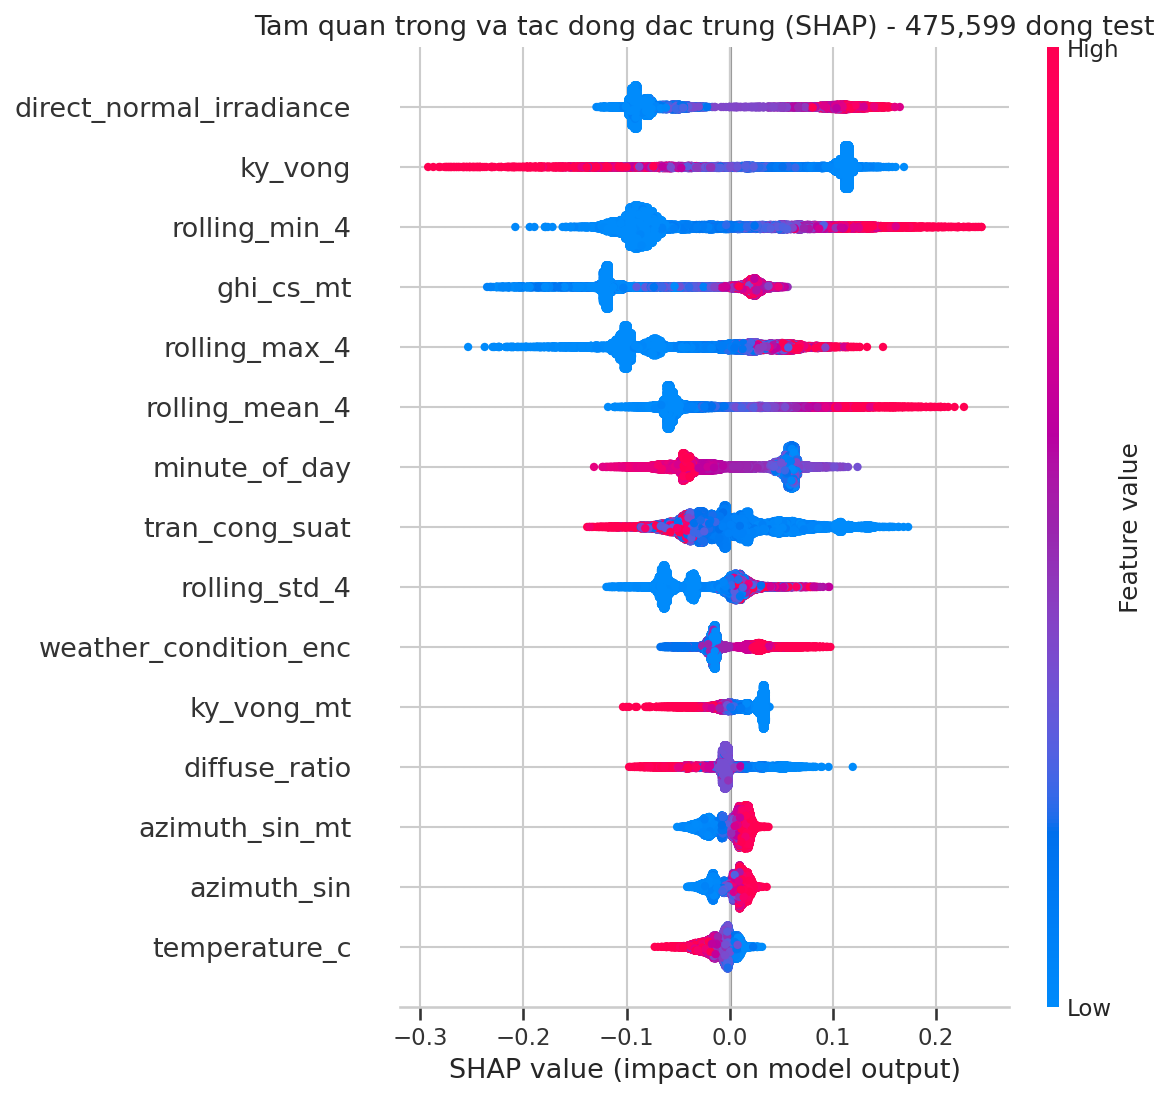
\includegraphics[width=\textwidth]{notebook_shap_beeswarm.png}
    
    
    \caption{Biểu đồ SHAP Beeswarm thể hiện tác động của các đặc trưng}
    \label{fig:shap_beeswarm}
\end{figure}

\FloatBarrier
\subsection{Giải thích ba dự báo cụ thể}

Tính chất cộng gộp của SHAP cho phép phân tích chi tiết từng trường hợp dự báo đơn lẻ. Notebook chọn ba trường hợp tương phản
trong tập test, ghi ở Bảng~\ref{tab:shap_local}.

\begin{table}[htbp]
\centering
\caption{Phân tích 3 trường hợp dự báo bằng SHAP cục bộ}
\label{tab:shap_local}
\small
\begin{tabular}{l r l r r}
\toprule
\textbf{Trường hợp} & \textbf{Trạm} & \textbf{Thời điểm} & \textbf{Thực tế (kWh)} & \textbf{Tổng SHAP} \\
\midrule
Đẩy dự báo lên  & $10$ & $30/03/2022$ $15{:}45$ & $6{,}6563$ & $+0{,}6839$ \\
Kéo dự báo xuống & $27$ & $28/01/2022$ $17{:}30$ & $6{,}2500$ & $-0{,}6976$ \\
Gần mức nền     & $30$ & $21/02/2022$ $10{:}00$ & $2{,}6484$ & $-0{,}0000$ \\
\bottomrule
\end{tabular}


\end{table}

Ba trường hợp này minh hoạ ba chế độ khác nhau của mô hình. Ở ca đẩy lên, ba đóng góp dương
lớn nhất đến từ \texttt{site\_id\_enc} ($+0{,}1385$), \texttt{diffuse\_ratio} ($+0{,}1163$) và
\texttt{direct\_normal\_irradiance} ($+0{,}1050$) --- trời quang buổi chiều, bức xạ trực tiếp
còn mạnh. Ở ca kéo xuống, đóng góp âm mạnh nhất là \texttt{rolling\_min\_4} ($-0{,}0692$) rồi
tới \texttt{diffuse\_ratio} ($-0{,}0566$): chiều muộn ngày nhiều mây, cả lịch sử một giờ gần
nhất cũng yếu. Ở ca gần nền, tổng đóng góp gần triệt tiêu vì các phần dương và âm cân nhau. Hai hình dạng thác tương
phản trình bày ở Hình~\ref{fig:shap_local}.

\begin{figure}[htbp]
    \centering
    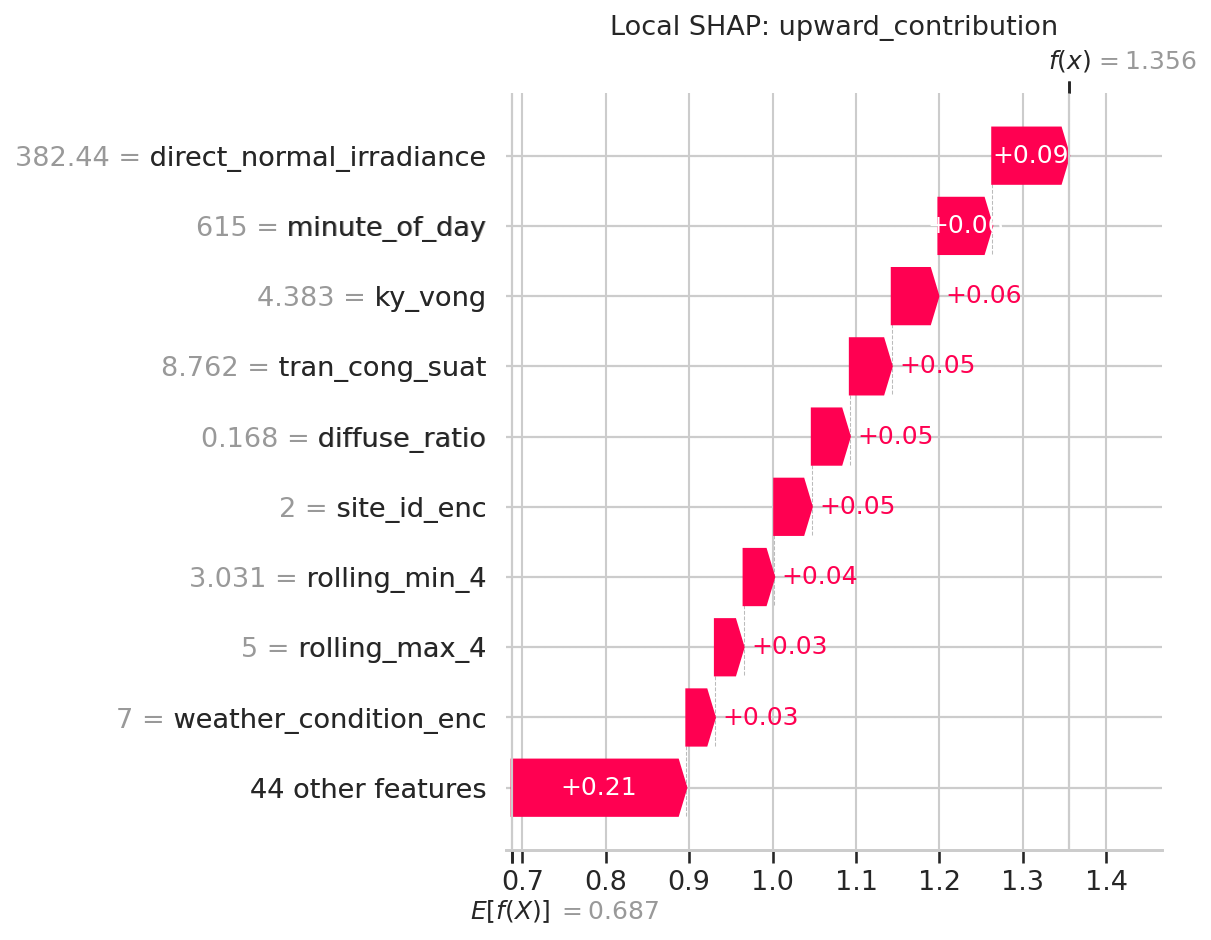
\includegraphics[width=0.86\textwidth]{local_shap_mae_h1_upward.png}\\[6pt]
    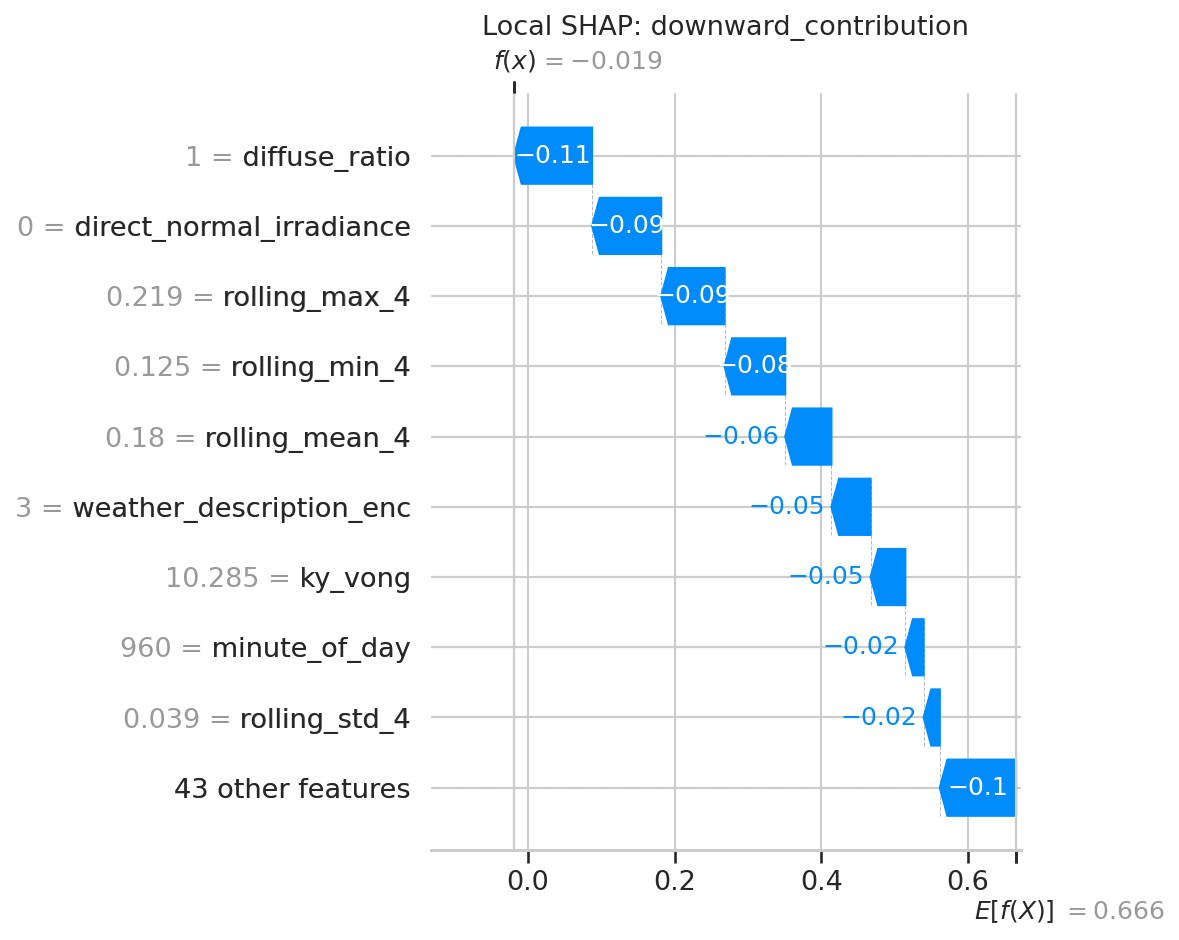
\includegraphics[width=0.86\textwidth]{local_shap_mae_h1_downward.png}
    
    
    \caption{Biểu đồ SHAP Waterfall giải thích hai trường hợp dự báo tương phản}
    \label{fig:shap_local}
\end{figure}

\FloatBarrier
\subsection{Giới hạn diễn giải}

SHAP quy phần đóng góp của đặc trưng vào dự báo của mô hình, không phải vào sản lượng
thật. Nó cho biết mô hình đã dựa vào đâu, không cho biết quan hệ nhân quả vật lý. Khi hai đặc
trưng tương quan cao, mà Mục~\ref{subsec:chan_doan_dac_trung} cho thấy có nhiều cặp như vậy, phần đóng góp có thể bị
chia giữa chúng theo cách phụ thuộc vào cấu trúc cây đã học, nên không nên đọc thứ hạng như một
xếp hạng tầm quan trọng vật lý.

\FloatBarrier
\FloatBarrier
\section{Ứng dụng Trực quan hoá Kết quả Học máy và Mô phỏng Tối ưu hóa}
\label{sec:streamlit_app}

Để đưa mô hình học máy vào phục vụ vận hành thực tế và hỗ trợ việc ra quyết định, toàn bộ kết quả dự báo, giải thích mô hình và phân tích kịch bản được đóng gói vào một ứng dụng web tương tác phát triển trên nền tảng Streamlit (\texttt{srcs/07\_dashboard/streamlit\_app/}). Ứng dụng đọc trực tiếp các tệp kết quả và siêu tham số từ \texttt{model\_config.json} của mô hình LightGBM, đảm bảo tính nhất quán tuyệt đối giữa giai đoạn huấn luyện và suy luận thực tế. Ứng dụng gồm 2 trang chức năng chuyên sâu:

\FloatBarrier
\subsection{Trang 1: Giám sát Chuỗi Thời gian và Giải thích Mô hình SHAP (\texttt{pages/1\_ML.py})}

Trang này tích hợp hai luồng nghiệp vụ:
\begin{itemize}[noitemsep]
    \item \textbf{Giám sát Dự báo Chuỗi Thời gian (Time-Series Forecasting):} Đặt đường thực tế cạnh đường dự báo theo từng trạm và từng khoảng thời gian (ở cả hai tầm dự báo $15$ phút và $1$ giờ), hiển thị bảng chỉ số kiểm định chi tiết (WAPE, RMSE, MAE, $R^2$) và biểu đồ đối chiếu kỹ năng dự báo với mô hình đường cơ sở Prophet (Hình~\ref{fig:streamlit1}).
    \item \textbf{Trực quan hóa Giải thích Mô hình (XAI TreeSHAP):} Hiển thị mức độ đóng góp toàn cục của 52 đặc trưng (Global Beeswarm Plot) và biểu đồ phân rã đóng góp cục bộ từng thời điểm (Local Waterfall Plot) do người dùng tùy chọn (Hình~\ref{fig:streamlit2}).
\end{itemize}

\begin{figure}[htbp]
    \centering
    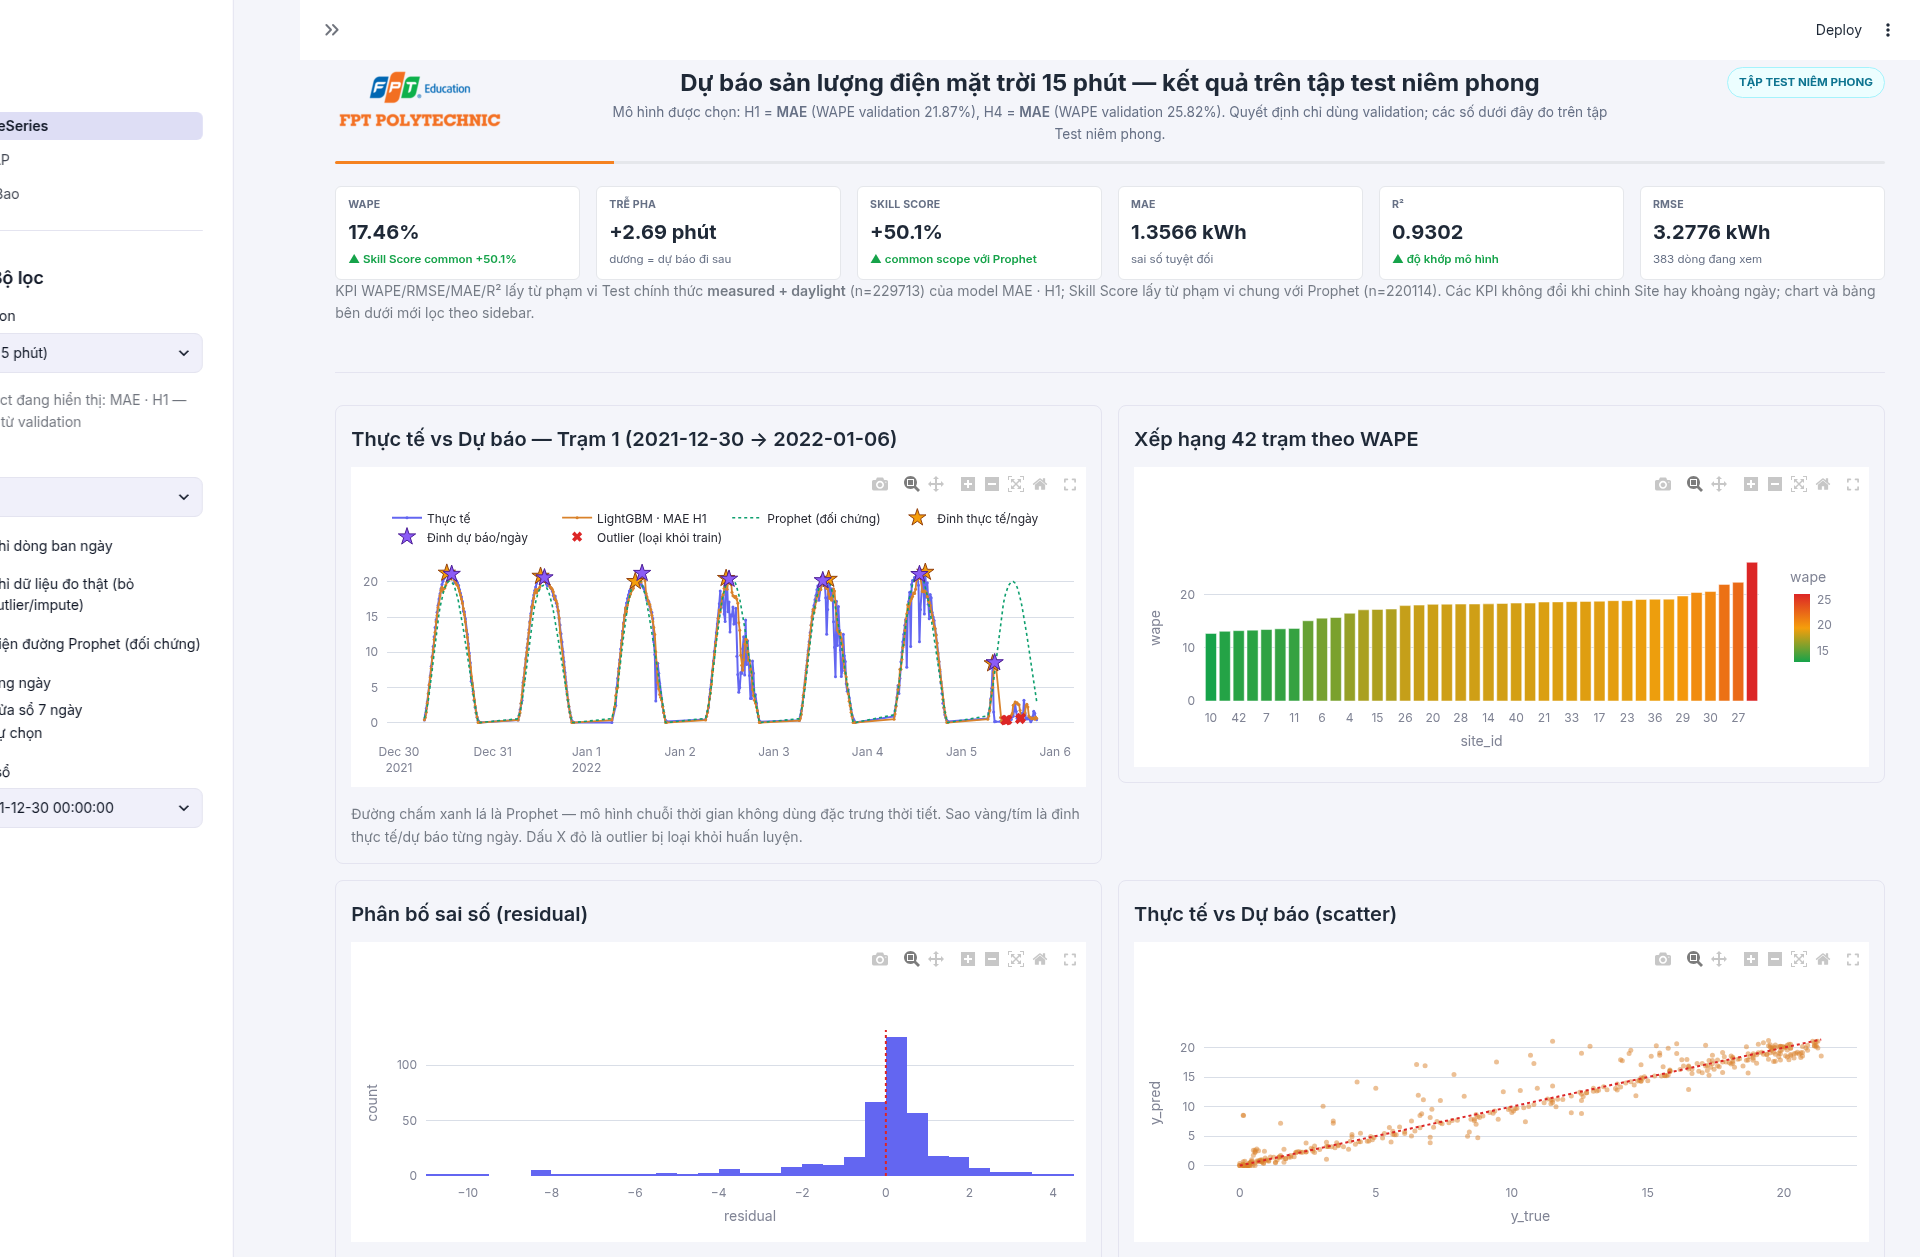
\includegraphics[width=\textwidth,height=0.48\textheight,keepaspectratio]{streamlit_1_timeseries.png}
    \caption[Giao diện Trang 1: Giám sát chuỗi thời gian]{Giao diện Trang 1: Giám sát chuỗi thời gian theo trạm trên Streamlit}
    \label{fig:streamlit1}
\end{figure}

\begin{figure}[htbp]
    \centering
    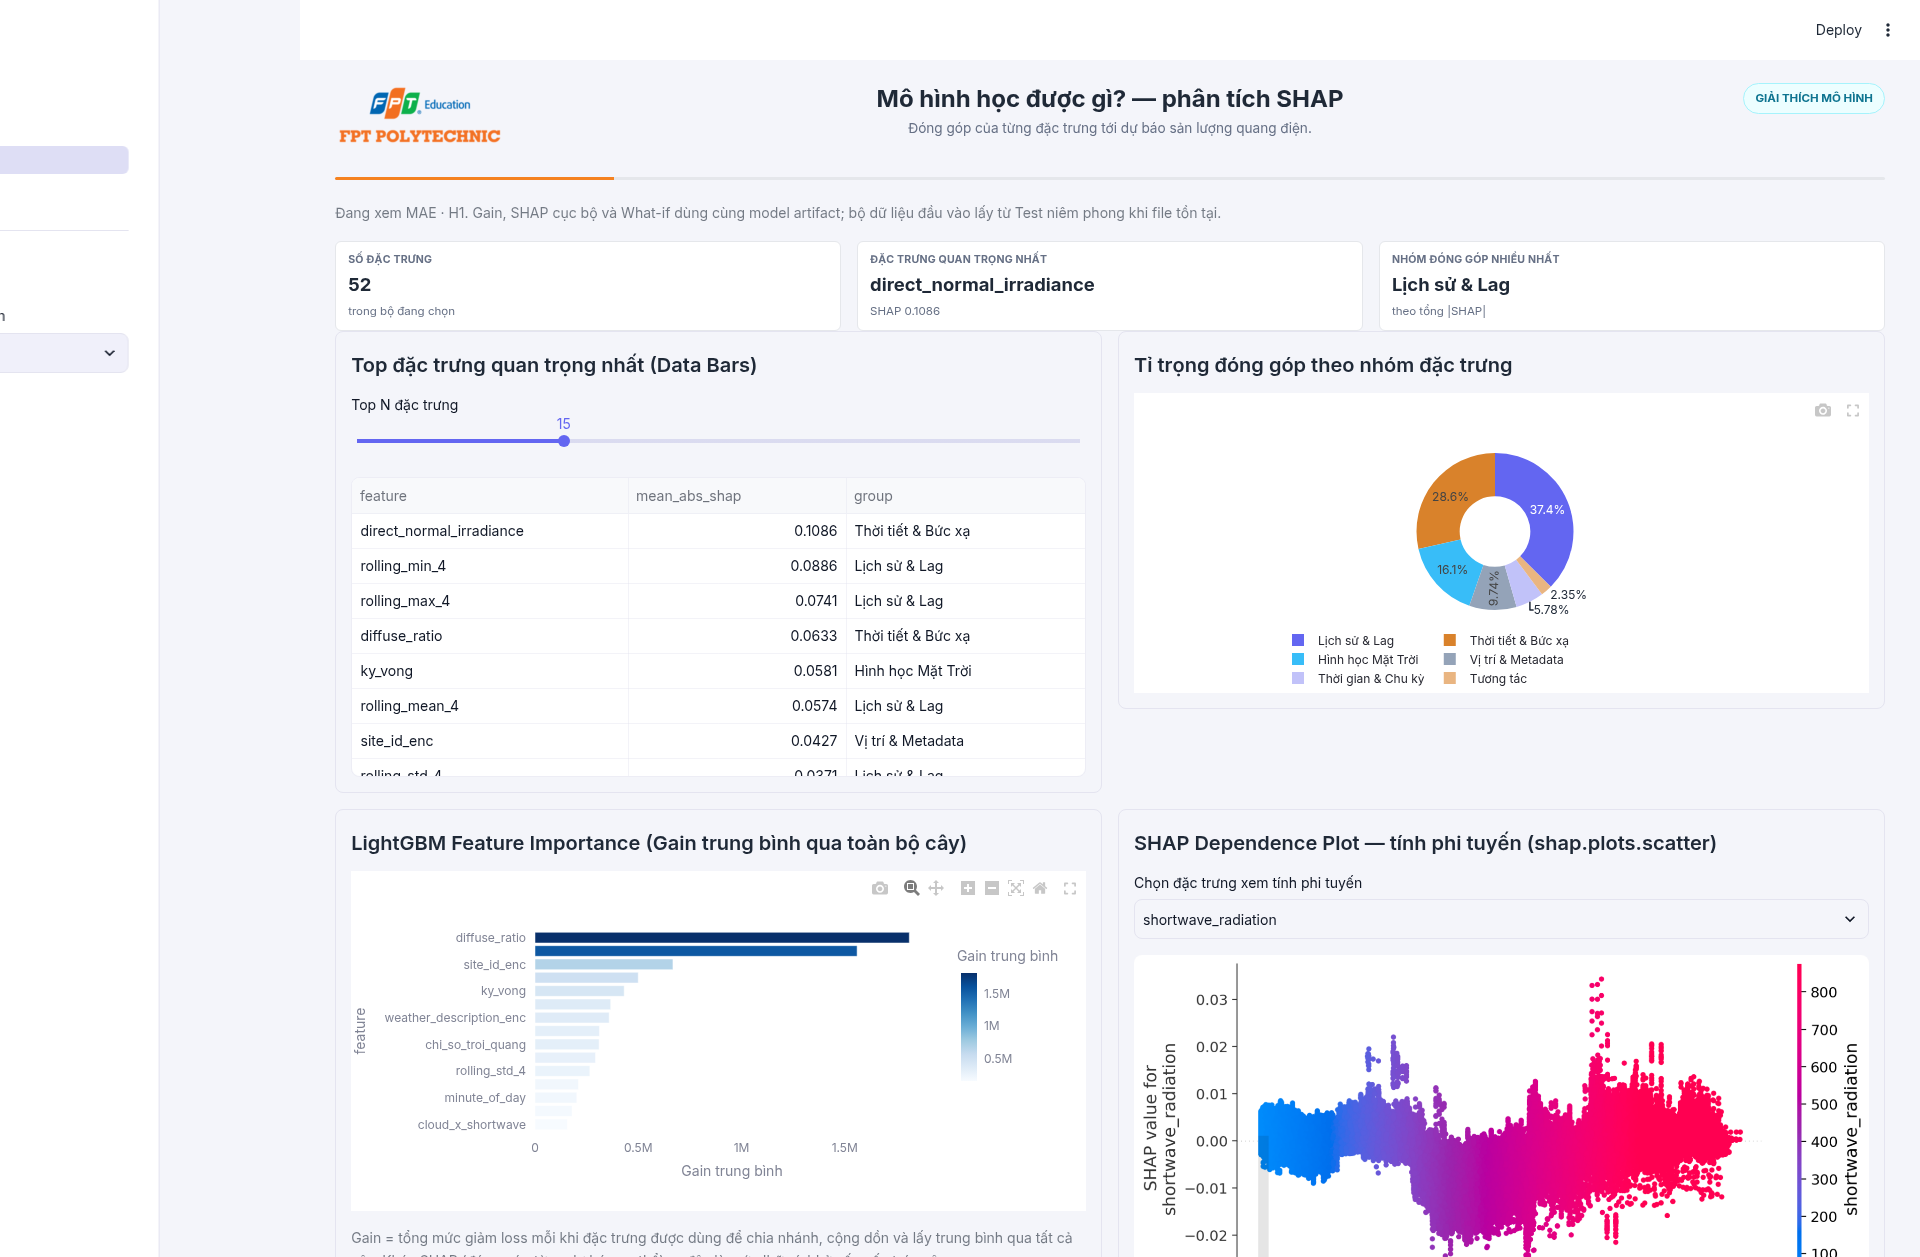
\includegraphics[width=\textwidth,height=0.48\textheight,keepaspectratio]{streamlit_2_shap.png}
    \caption[Giao diện Trang 1: Giải thích dự báo bằng SHAP]{Giao diện Trang 1: Giải thích dự báo bằng SHAP trên Streamlit}
    \label{fig:streamlit2}
\end{figure}

\FloatBarrier
\subsection{Trang 2: Dự báo Thực thi và Mô phỏng Giả định Tối ưu hóa (\texttt{pages/2\_What\_If.py})}

Trang này gọi trực tiếp module dịch vụ \texttt{forecast\_service.py} để sinh dự báo thời gian thực và cung cấp bảng điều khiển mô phỏng kịch bản tối ưu hóa giả định (Interactive What-If Scenario Simulation Dashboard) (Hình~\ref{fig:streamlit3}). 

Người dùng có thể chủ động kích hoạt các ô chọn (Checkboxes) tương ứng với 6 hạng mục giải pháp kỹ thuật (Hệ thống pin lưu trữ BESS $1\,\text{MW}/2{,}5\,\text{MWh}$, Khe hở thông gió làm mát mái $10-15\,\text{cm}$, Chuyển đổi bảo trì CBM theo cờ GMM-IF, Nâng khung nghiêng $15^\circ$ cho $970\,\text{kWp}$ mái bằng, Lịch rửa pin thông minh theo mưa, và Nâng cấp module TOPCon). Khi kích hoạt, hệ thống tự động tính toán lại toàn bộ các chỉ số vận hành và tài chính tức thời: Hệ số hiệu suất $PR$, Năng suất riêng, Doanh thu tiết kiệm ròng, Cắt giảm phát thải $\text{CO}_2$, Tổng chi phí đầu tư CapEx và Thời gian hoàn vốn có trọng số (Payback Period).

\begin{figure}[htbp]
    \centering
    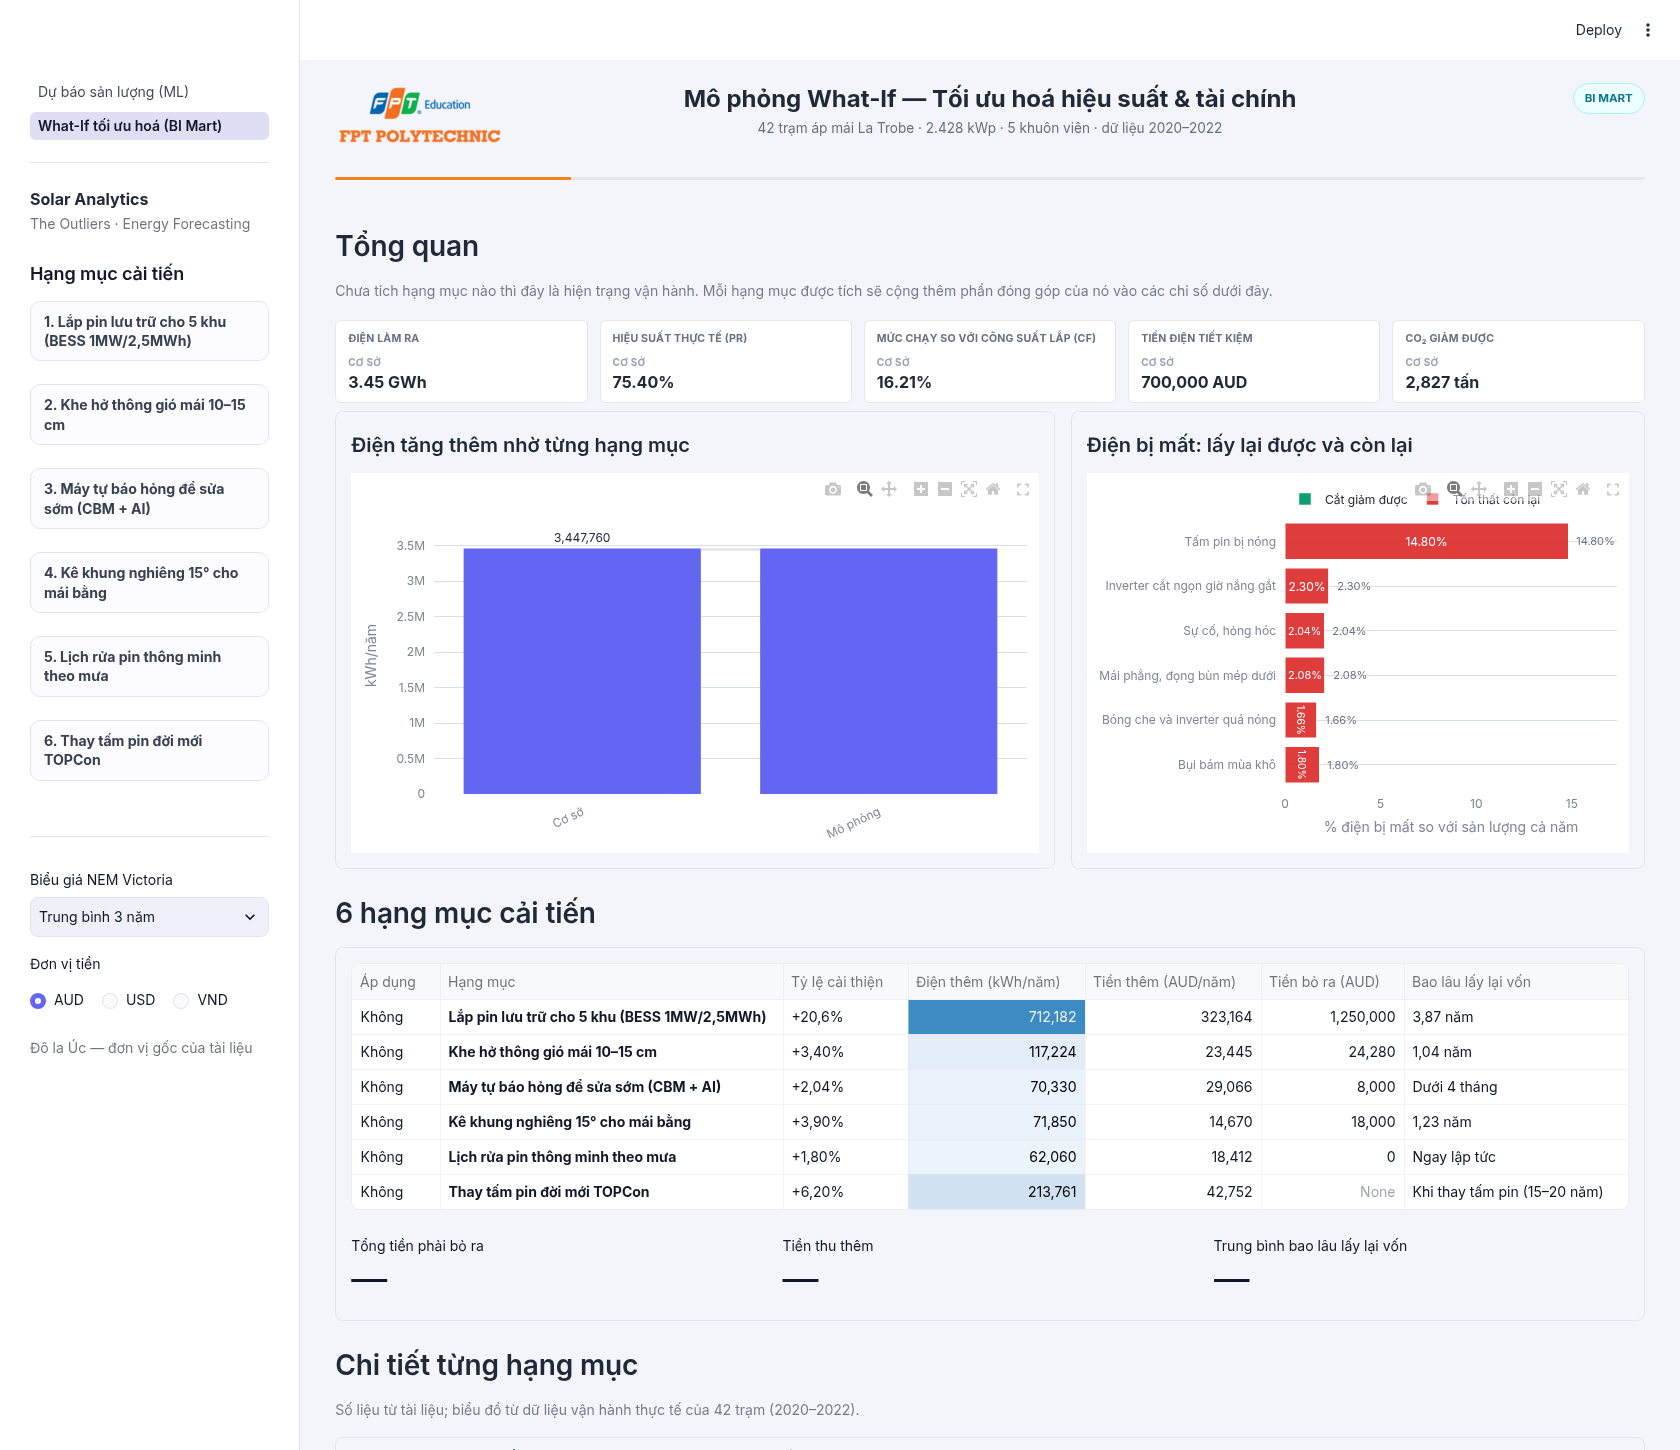
\includegraphics[width=\textwidth,height=0.52\textheight,keepaspectratio]{streamlit_3_du_bao.png}
    \caption[Giao diện Trang 2: Mô phỏng kịch bản tối ưu hóa What-If]{Giao diện Trang 2: Dự báo và mô phỏng tối ưu hóa What-If Analysis trên Streamlit}
    \label{fig:streamlit3}
\end{figure}

\FloatBarrier
\section{Tổng kết Kỹ thuật Mô hình Học máy}
\label{sec:tong_ket_ky_thuat_ml}

Mục này tổng kết các kết quả kỹ thuật của quy trình học máy, các phát hiện then chốt và giới hạn kỹ thuật của mô hình:

\FloatBarrier
\subsection{Kết quả Đạt được Về Mặt Kỹ thuật}

Quy trình đã xây dựng thành công một mô hình LightGBM dùng chung cho $40$ trạm quang điện áp mái (sau khi loại 2 trạm đối chứng khí tượng), đạt $\text{WAPE} = 17{,}73\%$ ở tầm $15$ phút ($R^2 = 0{,}9283$) và $22{,}58\%$ ở tầm $1$ giờ ($R^2 = 0{,}8964$) trên tập test niêm phong ở phạm vi đo thật ban ngày. So với mô hình đường cơ sở Prophet trên cùng tập dữ liệu kiểm tra, chỉ số kỹ năng dự báo (Skill Score) của LightGBM đạt mức vượt trội $+48{,}73\%$ ở tầm ngắn hạn và $+35{,}89\%$ ở tầm một giờ.

Năm rào chắn chống rò rỉ dữ liệu ở Mục~\ref{subsec:nam_rao_chan} đã được kiểm chứng nghiêm ngặt bằng số liệu: phép ghép thời tiết nhân quả đưa số dòng vi phạm rò rỉ tương lai về $0$; thống kê quy mô trạm được tính toán độc lập theo từng fold; cận cắt được suy luận từ phân vị của tập huấn luyện; và tập test chỉ được mở duy nhất một lần ở bước đánh giá cuối cùng.

\FloatBarrier
\subsection{Hạn chế Kỹ thuật của Mô hình}

\begin{itemize}[noitemsep]
    \item \textbf{Dữ liệu khí tượng độc lập nhỏ hơn con số 42:} Bốn mươi hai trạm phân bố tại 5 cơ sở, do đó các trạm trong cùng khuôn viên chia sẻ chung một chuỗi dữ liệu khí tượng viễn thám ERA5.
    \item \textbf{Sai số phân bố chưa hoàn toàn đồng đều giữa các trạm:} $\text{WAPE}$ dao động từ $12{,}69\%$ tới $26{,}06\%$ ở tầm H1, do cấu hình lắp đặt và mức độ che bóng cục bộ của từng trạm áp mái có sự khác biệt.
    \item \textbf{Độ trễ pha còn tồn tại ở mức nhỏ:} Cổng đo ghi nhận độ trễ trung bình $+2{,}38$ phút trên toàn tập kiểm định, nằm trong ngưỡng cho phép $\pm 5$ phút nhưng vẫn nghiêng nhẹ về phía trễ.
    \item \textbf{Độ phân giải thời tiết gốc là 1 giờ:} Việc nội suy dữ liệu thời tiết ERA5 từ 1 giờ xuống 15 phút chưa phản ánh tức thời các biến động mây tích cục bộ trong vài phút.
\end{itemize}

\FloatBarrier
\subsection{Hướng phát triển}
\label{subsec:huong_phat_trien}

Ba việc cụ thể, xếp theo mức dễ làm:

\begin{enumerate}
    \item Mở rộng miền tìm kiếm ở chỗ chạm biên, nâng cận trên của \texttt{reg\_lambda}.
    \item Chạy hai cấu hình đối chứng còn thiếu để tách phần đóng góp của nhóm đặc trưng khí
    tượng: một LightGBM bỏ hết biến khí tượng, và một Prophet có biến ngoại sinh.
    \item Xử lý phần khác biệt giữa các trạm, hoặc bằng đặc trưng riêng cho trạm, hoặc bằng
    cách hiệu chỉnh đầu ra theo từng trạm sau khi dự báo.
\end{enumerate}

% Danh mục tham khảo luôn bắt đầu ở trang mới, không dính vào cuối mục cuối cùng.

% Tra float ve mac dinh LaTeX cho cac chuong con lai.
\setcounter{topnumber}{2}
\setcounter{bottomnumber}{1}
\setcounter{totalnumber}{3}
\renewcommand{\topfraction}{0.7}
\renewcommand{\bottomfraction}{0.3}
\renewcommand{\textfraction}{0.2}
\renewcommand{\floatpagefraction}{0.5}

\newpage

\chapter{Kết luận và Hướng phát triển}
\label{chap:conclusion}

\section{Bóc tách 6 Điểm nghẽn Vận hành Cốt lõi của Danh mục Trạm}
\label{sec:bottlenecks}

Qua quá trình phân tích dữ liệu chuyên sâu trên Kho dữ liệu đa chiều Supabase, hệ thống Dashboard Tableau và mô hình nhận diện dị thường GMM--IF, nhóm nghiên cứu đã lượng hóa được 6 điểm nghẽn kỹ thuật và vận hành cốt lõi làm thất thoát sản lượng của 42 trạm quang điện áp mái tại Đại học La Trobe:

\begin{enumerate}[label=\arabic*., leftmargin=*]
    \item \textbf{Suy hao do Nhiệt độ Tế bào Quang điện Quá cao ($Loss_{\text{temp}} = 14{,}80\%$):} 
    Do đa số các tấm pin được lắp áp sát mặt mái tôn mà không có khoảng hở đối lưu nhiệt, vào các tháng mùa hè bang Victoria (tháng 12 đến tháng 2), nhiệt độ bề mặt tấm pin ($T_{\text{cell}}$) thường xuyên vượt ngưỡng $65^\circ\text{C} - 72^\circ\text{C}$. Với hệ số nhiệt $\gamma = -0{,}38\%/^\circ\text{C}$, tổn thất nhiệt độ làm bốc hơi $\mathbf{510.268\,\text{kWh/năm}}$ (tương đương thiệt hại hơn $102.000\,\text{AUD/năm}$).

    \item \textbf{Tổn thất Cắt ngọn Biến tần ($Loss_{\text{clip}} = 2{,}30\%$):} 
    Tỷ lệ thiết kế công suất mảng pin DC lớn hơn định mức biến tần AC ($\text{ILR} = 1{,}25$) khiến các trạm phát bị xén công suất đỉnh (Flat-top clipping) từ 11:30 đến 14:00 vào những ngày nắng gắt, gây thất thoát $\mathbf{79.298\,\text{kWh/năm}}$.

    \item \textbf{Bám bụi Bề mặt Tấm pin Mùa Khô ($Loss_{\text{soiling}} = 1{,}80\%$):} 
    Trong các tháng khô hạn kéo dài tại bang Victoria, bụi bẩn, phấn hoa và tạp chất khí quyển bám dính trên bề mặt kính quang học làm suy giảm $\mathbf{62.060\,\text{kWh/năm}}$ (tương đương tổn thất $12.412\,\text{AUD/năm}$ tiền điện). Bên cạnh đó, việc thực hiện rửa pin thủ công định kỳ theo lịch cố định mà không tham chiếu dữ liệu dự báo mưa thường gây lãng phí lớn về chi phí nhân công O\&M.

    \item \textbf{Hiện tượng Ngắt mạch Quá áp Lưới Hạ thế (Grid Overvoltage Tripping):} 
    Theo tiêu chuẩn Úc AS/NZS 4777.2, khi điện áp hòa lưới $10$ phút trung bình vượt ngưỡng $V_{10\text{min}} \ge 258\,\text{V}$, biến tần buộc phải ngắt mạch khẩn cấp. Hiện tượng này phát sinh tập trung vào các buổi trưa hè khi phụ tải khuôn viên thấp nhưng điện mặt trời phát cực đại, được bóc tách chính xác qua mã cờ \texttt{PHYSICAL\_LOW\_ENERGY\_STRONG\_SUN}.

    \item \textbf{Cảnh báo Giả và Độ trễ Phát hiện Sự cố trong Quy trình O\&M Truyền thống:} 
    Quy trình kiểm tra định kỳ thủ công khiến thời gian phát hiện sự cố (MTTD) kéo dài từ 2 đến 4 tuần, trong khi các phương pháp lọc ngưỡng tĩnh truyền thống tạo ra tỷ lệ báo động giả cao trong những ngày nhiều mây.

    \item \textbf{Thiếu Công cụ Mô phỏng Động Đa Kịch bản (What-If Analysis):} 
    Đơn vị quản lý tài sản thiếu một công cụ trực quan để đánh giá tương tác giữa các phương án đầu tư cải tạo kỹ thuật với dòng tiền thu hồi vốn và hiệu quả cắt giảm phát thải $\text{CO}_2$.
\end{enumerate}

\section{Chi tiết 6 Hạng mục Đề xuất Cải tiến Kỹ thuật Đã Kiểm toán}
\label{sec:audited_proposals}

Dựa trên việc bóc tách chính xác nguyên nhân gốc rễ, nhóm đề xuất 6 giải pháp kỹ thuật có tính khả thi cao, được kiểm toán định lượng chi tiết về mặt kỹ thuật và tài chính:

\begin{table}[H]
\centering
\caption{Tổng hợp 6 hạng mục đề xuất cải tiến kỹ thuật đã kiểm toán (Audited Proposals)}
\label{tab:six_proposals_summary}
\footnotesize
\renewcommand{\arraystretch}{1.3}
\begin{tabularx}{\textwidth}{@{} c >{\raggedright\arraybackslash}p{4.2cm} >{\raggedright\arraybackslash}X c c c @{}}
\toprule
\textbf{STT} & \textbf{Hạng Mục Đề Xuất Kỹ Thuật} & \textbf{Cơ Chế Tác Động Vật Lý} & \textbf{Điện Thu Hồi} & \textbf{Lợi Ích Ròng} & \textbf{Hoàn Vốn} \\
\midrule
1 & \textbf{Hệ thống Pin Lưu trữ BESS} \newline ($1\,\text{MW} / 2{,}5\,\text{MWh}$ tại 5 Campus) & Hấp thu toàn bộ điện cắt ngọn DC, xả vào giờ cao điểm giá điện tối và chống quá áp lưới AS/NZS 4777.2. & $+712.182\,\text{kWh}$ & $+323.164\,\text{AUD}$ & $3{,}87\,\text{năm}$ \\
\midrule
2 & \textbf{Khe hở Thông gió Mái $10-15\,\text{cm}$} \newline (Chuẩn AS/NZS 5033) & Tạo luồng đối lưu khí tự nhiên làm mát mặt lưng tấm pin, hạ nhiệt độ cell $-8{,}0^\circ\text{C}$. & $+117.224\,\text{kWh}$ & $+23.445\,\text{AUD}$ & $1{,}04\,\text{năm}$ \\
\midrule
3 & \textbf{Chuyển đổi Bảo trì CBM \& AI} \newline (6 mã cờ GMM--IF) & Rút ngắn thời gian phát hiện sự cố $\text{MTTD} < 1\,\text{h}$, điều phối sửa chữa theo điều kiện hư hỏng thực tế. & $+70.330\,\text{kWh}$ & $+29.066\,\text{AUD}$ & $< 4\,\text{tháng}$ \\
\midrule
4 & \textbf{Nâng Khung nghiêng chữ A $15^\circ$} \newline (Cho $970\,\text{kWp}$ mái bằng Hướng Bắc) & Tối ưu hóa góc hứng bức xạ mặt trời mùa đông và tạo độ dốc thoát nước tự làm sạch bề mặt pin. & $+71.850\,\text{kWh}$ & $+14.670\,\text{AUD}$ & $1{,}68\,\text{năm}$ \\
\midrule
5 & \textbf{Lịch Rửa Pin Thông Minh theo Mưa} \newline (Khí tượng ERA5 Precipitation) & Rửa khi chuỗi ngày khô hạn $\ge 21\,\text{ngày}$ và $\sum P_{\text{mưa}} < 2\,\text{mm}$; cắt 3 lần rửa thừa/năm, tiết kiệm 6.000 AUD nhân công. & $+62.060\,\text{kWh}$ & $+18.412\,\text{AUD}$ & Tức thì \\
\midrule
6 & \textbf{Nâng cấp Module N-type TOPCon} \newline (Tùy chọn dài hạn kỳ đại tu) & Thay thế module cũ bằng công nghệ TOPCon hiệu suất $22{,}5\%$, hệ số nhiệt thấp $\gamma = -0{,}30\%/^\circ\text{C}$. & $+213.761\,\text{kWh}$ & $+42.752\,\text{AUD}$ & Tích hợp \\
\bottomrule
\end{tabularx}
\end{table}

\section{Bảng Tổng hợp Mô phỏng Tối ưu hóa What-If Toàn Danh mục}
\label{sec:what_if_fleet_matrix}

Khi tích hợp đồng bộ các giải pháp cải tiến kỹ thuật thông qua Bảng điều khiển mô phỏng tương tác Streamlit What-If Simulator (\texttt{pages/2\_What\_If.py}), bức tranh tổng thể về hiệu suất kỹ thuật, giá trị kinh tế và bảo vệ môi trường của toàn bộ danh mục 42 trạm được nâng cấp vượt bậc so với đường cơ sở ban đầu (Bảng~\ref{tab:what_if_fleet_comparison}):

\begin{table}[H]
\centering
\caption{Ma trận so sánh toàn diện Hiện trạng (Baseline) vs Sau Tối ưu hóa (Optimized)}
\label{tab:what_if_fleet_comparison}
\small
\renewcommand{\arraystretch}{1.3}
\begin{tabularx}{\textwidth}{@{} >{\raggedright\arraybackslash}p{4.8cm} >{\raggedright\arraybackslash}X >{\raggedright\arraybackslash}X >{\raggedright\arraybackslash}X @{}}
\toprule
\textbf{Chỉ Số Đánh Giá (Fleet KPIs)} & \textbf{Hiện Trạng (Baseline)} & \textbf{Sau Tối Ưu (Optimized)} & \textbf{Mức Cải Thiện Ròng} \\
\midrule
\textbf{Tổng Sản Lượng Điện Phát} & $3{,}45\,\text{GWh/năm}$ ($3.447.760\,\text{kWh}$) & $4{,}70\,\text{GWh/năm}$ ($4.695.534\,\text{kWh}$) & $\mathbf{+1{,}25\,\text{GWh/năm}}$ ($\mathbf{+36{,}18\%}$) \\
\textbf{Hệ Số Hiệu Suất ($PR$)} & $75{,}40\%$ (Class B Tiêu chuẩn) & $88{,}62\%$ (Class A Quốc tế) & $\mathbf{+13{,}22\,\text{điểm \%}}$ ($+17{,}54\%$) \\
\textbf{Hệ Số Công Suất ($CF$)} & $16{,}21\%$ & $22{,}07\%$ & $\mathbf{+5{,}86\,\text{điểm \%}}$ ($+36{,}18\%$) \\
\textbf{Năng Suất Riêng (Specific Yield)} & $1.420\,\text{kWh/kWp/năm}$ & $1.934\,\text{kWh/kWp/năm}$ & $\mathbf{+514\,\text{kWh/kWp/năm}}$ \\
\textbf{Doanh Thu Tiết Kiệm Tiền Điện} & $700.000\,\text{AUD/năm}$ & $1.151.509\,\text{AUD/năm}$ & $\mathbf{+451.509\,\text{AUD/năm}}$ ($\mathbf{+64{,}50\%}$) \\
\textbf{Cắt Giảm Phát Thải $\text{CO}_2$} & $2.827\,\text{tấn/năm}$ ($0{,}82\,\text{kg/kWh}$) & $3.850\,\text{tấn/năm}$ & $\mathbf{+1.023\,\text{tấn CO}_2\text{/năm}}$ \\
\midrule
\textbf{Tổng Vốn Đầu Tư (CapEx)} & — & $\mathbf{1.300.280\,\text{AUD}}$ & BESS: $1{,}25\,\text{M}$, Khác: $50{,}28\,\text{k}$ \\
\textbf{Thời Gian Hoàn Vốn (Payback)} & — & $\mathbf{3{,}15\,\text{NĂM}}$ & $\mathbf{\text{ROI} > 270\%}$ (Vòng đời 20 năm) \\
\bottomrule
\end{tabularx}
\end{table}

\section{Định hướng Chiến lược Phát triển trong Tương lai}
\label{sec:strategic_roadmap}

Nhằm tiếp tục phát huy tối đa giá trị của nền tảng dữ liệu và mô hình AI, dự án vạch ra lộ trình chiến lược phát triển theo 3 mũi nhọn:

\begin{enumerate}[label=\arabic*., leftmargin=*]
    \item \textbf{Tham gia Thị trường Điện Giao ngay NEM AEMO 5 Phút (Energy Arbitrage \& FCAS):} 
    Kết hợp mô hình dự báo LightGBM tầm siêu ngắn hạn với hệ thống pin BESS để tham gia thị trường dịch vụ phụ trợ tần số (FCAS) và chiến lược chênh lệch giá (Arbitrage) trên thị trường điện quốc gia Úc (NEM), chủ động sạc pin vào những khung giờ giá điện âm giữa trưa và xả phát vào giờ cao điểm tối ($18:00 - 20:00$) khi giá điện chạm trần thị trường ($> 300\,\text{AUD/MWh}$).

    \item \textbf{Thương mại hóa Tín chỉ Giảm phát thải Carbon Úc (ACCUs):} 
    Tận dụng dữ liệu đo đếm minh bạch $100\%$ từ DWH để đăng ký phương pháp luận tạo tín chỉ carbon theo Cơ chế Tín chỉ Carbon Úc (Australian Carbon Credit Units -- ACCUs), mở ra nguồn doanh thu mới từ thị trường chứng chỉ xanh.

    \item \textbf{Tự động hóa Quy trình MLOps và Điều độ Bảo trì Dự báo Trước (Forecasting-Driven O\&M):} 
    Đóng gói toàn bộ pipeline thành các luồng điều phối tự động (Airflow / Prefect), tích hợp công nghệ Edge AI vào các bộ điều khiển RTU tại trạm, và tự động liên kết kết quả dự báo thời tiết cực đoan để lên lịch làm mát biến tần và phân công kỹ sư bảo trì trước khi sự cố xảy ra.
\end{enumerate}
% ====================================================================
%  PHỤ LỤC A: KẾ HOẠCH THỰC HIỆN VÀ PHÂN CÔNG NHIỆM VỤ
% ====================================================================
\chapter*{Phụ lục A: Kế hoạch Thực hiện và Phân công Nhiệm vụ}
\addcontentsline{toc}{chapter}{Phụ lục A: Kế hoạch Thực hiện và Phân công Nhiệm vụ}
\label{app:kehoach}
\renewcommand{\thetable}{A.\arabic{table}}
\setcounter{table}{0}
\renewcommand{\thefigure}{A.\arabic{figure}}
\setcounter{figure}{0}

\section*{A.1. Lộ trình Thực hiện 14 Tuần (Sprint Timeline)}
\begin{table}[H]
\centering
\caption{Lộ trình 14 tuần thực hiện dự án theo 8 Sprints chuẩn hóa theo CLO}
\label{tab:sprint_timeline}
\small
\renewcommand{\arraystretch}{1}
\begin{tabularx}{\textwidth}{@{} l l p{3.2cm} p{3.8cm} X @{}}
\toprule
\textbf{Sprint} & \textbf{Thời Gian} & \textbf{Quy Trình (CLO)} & \textbf{Nội Dung Trọng Tâm} & \textbf{Sản Phẩm Đầu Ra (Deliverables)} \\
\midrule
Sprint 1 & Tuần 1 -- 2 & Bước 1: Thu thập \newline (\textbf{CLO1}) & Khởi tạo \& Thu thập dữ liệu thô & Project Charter, Backlog Jira, GitHub Repo, 2,73 triệu dòng dữ liệu La Trobe University, Open-Meteo API, AEMO VIC RRP. \\
Sprint 2 & Tuần 3 -- 4 & Bước 1.5: Lưu trữ \newline (\textbf{CLO2}) & Xây dựng Pipeline ETL \& Data Warehouse & DDL Supabase PostgreSQL, Lược đồ Galaxy Schema, Staging \& Buffer Layer, DVC, S3 Storage, CI/CD GitHub Actions. \\
Sprint 3 & Tuần 5 -- 6 & Bước 2: Làm sạch \newline (\textbf{CLO3}) & Làm sạch dữ liệu (Data Cleaning) & Thuật toán Hybrid Imputation vá dữ liệu khuyết, lọc dị thường Rolling IQR \& GMM--IF, cờ phân loại \texttt{gmm\_if\_outlier\_flag}. \\
Sprint 4 & Tuần 7 -- 8 & Bước 3: Chuyển đổi \newline (\textbf{CLO4}) & Biến đổi \& Làm giàu dữ liệu (Transformation) & Materialized Views \texttt{bi\_mart} và \texttt{ml\_mart}, logic tính toán PR, Temperature Loss, quy đổi tài chính theo giá AEMO Victoria. \\
Sprint 5 & Tuần 9 -- 10 & Bước 4: Phân tích \newline (\textbf{CLO5}) & Khám phá dữ liệu chuyên sâu (EDA) & Kiểm định tính dừng ADF Test, biểu đồ tự tương quan ACF/PACF, ma trận tương quan thời tiết và phân tích đa biến. \\
Sprint 6 & Tuần 11 & Bước 5: Trực quan \newline (\textbf{CLO6}) & Trực quan hóa kết quả phân tích & Bộ 3 Dashboard Tableau hoàn chỉnh (Executive Snapshot, Technical Deep-Dive, Solar Asset \& Weather Impact), \texttt{Preferences.tps}. \\
Sprint 7 & Tuần 12 -- 13 & Bước 6: Dự báo \newline (\textbf{CLO7}) & Mô hình hóa \& Dự báo dữ liệu & Pipeline LightGBM/ARIMA, tối ưu Optuna, giải thích mô hình SHAP, Web App Streamlit (Interactive What-If Analysis). \\
Sprint 8 & Tuần 14 & Tổng kết \newline (\textbf{CLO8}) & Hoàn thiện tài liệu dự án & Báo cáo tốt nghiệp hoàn chỉnh, tài liệu kiến trúc kỹ thuật DWH, video demo và đóng gói mã nguồn nghiệm thu. \\
\bottomrule
\end{tabularx}


\end{table}

\section*{A.2. Ma trận Phân công Trách nhiệm Thành viên (RACI Matrix)}

\begin{table}[H]
\centering
\caption{Phân công nhiệm vụ và khối lượng hoàn thành của các thành viên}
\label{tab:member_assignment}
\small
\renewcommand{\arraystretch}{1}
\begin{tabularx}{\textwidth}{@{} l l X c @{}}
\toprule
\textbf{Thành Viên} & \textbf{MSSV} & \textbf{Phạm Vi Công Việc Chính} & \textbf{Tỷ Lệ (\%)} \\
\midrule
\textbf{Nguyễn Vũ Nhựt} & PS44442 & 
\textbf{Trưởng nhóm (Team Leader / PM):} Điều phối tiến độ dự án (Sprint/Jira), kiểm soát quy chuẩn kỹ thuật hệ thống, thực hiện Code Review, kiểm duyệt chất lượng dữ liệu và rà soát, hoàn thiện báo cáo tổng thể. & 
$100\%$ \\
\midrule
\textbf{Ngô Tấn Đạt} & PS44589 & 
\textbf{Lead Data Architect / AI:} Thiết kế kiến trúc Pipeline ETL/MLOps, quản lý cơ sở dữ liệu và hạ tầng DWH (Supabase/PostgreSQL), phát triển API, nghiên cứu và huấn luyện mô hình (GMM--IF, LightGBM/Optuna/SHAP). & 
$100\%$ \\
\midrule
\textbf{Lê Công Toàn} & PS44145 & 
Xây dựng module Tiền xử lý dữ liệu (Transform), nghiên cứu cơ sở toán học và triển khai thuật toán Điền khuyết nhân quả (Causal Cascade Imputation), đồng bộ dữ liệu đa tần số thời gian (15m vs 1h). & 
$100\%$ \\
\midrule
\textbf{Nguyễn Văn Sỹ} & PS43671 & 
Phân tích Khám phá Dữ liệu (EDA), khai phá insight từ mẫu hình phát điện, phát triển Hệ thống Dashboard Quản trị trên Tableau Desktop, thiết kế UI/UX theo bảng màu ngữ nghĩa và xây dựng Calculated Fields phức hợp. & 
$100\%$ \\
\midrule
\textbf{Nguyễn Xuân Hùng} & PS44527 & 
Quản lý tài liệu nghiệp vụ và đặc tả kỹ thuật, kiểm định và đối soát tính toàn vẹn dữ liệu (Data Quality \& Verification), hỗ trợ triển khai cấu trúc kho dữ liệu và tổng hợp kết quả kiểm thử. & 
$100\%$ \\
\bottomrule
\end{tabularx}


\end{table}

% ====================================================================
%  PHỤ LỤC B: CẤU TRÚC GÓI MÃ NGUỒN 
% ====================================================================
\chapter*{Phụ lục B: Cấu trúc Gói Mã nguồn}
\addcontentsline{toc}{chapter}{Phụ lục B: Cấu trúc Gói Mã nguồn}
\label{app:code}

Toàn bộ mã nguồn của dự án được tổ chức theo cấu trúc module hóa hướng đối tượng chuẩn công nghiệp, cho phép tái lập 100\% kết quả nghiên cứu:

\begin{lstlisting}[basicstyle=\ttfamily\scriptsize, breaklines=false, numbers=none, caption={Sơ đồ cấu trúc cây thư mục mã nguồn của dự án The Outliers}]
datn_outlier_hs_nlmt/
|-- data/
|   |-- raw/                             # Du lieu goc UNISOLAR & API
|   |-- staging_buffers/                 # Du lieu dem resample 15 phut
|   `-- mlmart_base/
|       `-- v5_final_cleaned.parquet     # Tap hop nhat 2,73M dong (ML Mart)
|-- docs/
|   `-- scrum_8_project_delivery_defense/# Tai lieu nghien cuu & bao ve
|-- reports/
|   |-- DATN_REPORT_FINAL_01.tex         # Bao cao tong hop chinh thuc
|   |-- Section1.tex -> Section7.tex     # Cac chuong bao cao doc lap
|   |-- figures/                         # So do kien truc & Dashboard
|   `-- images/                          # Bieu do EDA, SHAP & research
`-- srcs/
    |-- 00_database/                     # DDL tao Supabase DWH (Galaxy)
    |-- 00_utils/                        # Ket noi CSDL & Object Storage
    |-- 01_extract/                      # Crawler Kaggle & Weather API
    |-- 02_transform/
    |   |-- 01_run_transform_buffers.py  # Resample 15m & dien khuyet
    |   `-- 02_generate_outliers/        # Thuat toan GMM-IF gan 6 ma loi
    |-- 03_load/                         # Nap vao Supabase Data Warehouse
    |-- 04_build_data_marts/             # Tao BI Mart & Views cho Tableau
    |-- 05_machine_learning/
    |   |-- pipeline/
    |   |   |-- core/                    # Metric WAPE, Huber, L1 Loss
    |   |   |-- stages/ (s01 -> s10)     # 10 buoc pipeline ML tu dong
    |   |   `-- actions/                 # Optuna 20 trials & Baseline
    |-- 06_run_pipeline/                 # Orchestrator dieu phoi toan bo
    `-- 07_dashboard/
        |-- app.py                       # Ung dung Streamlit tuong tac
        |-- forecast_service.py          # Dich vu du bao realtime doc lap
        `-- pages/                       # Cac trang (TimeSeries, SHAP, DuBao)
\end{lstlisting}


% ====================================================================
%  PHỤ LỤC C: SƠ ĐỒ VÒNG ĐỜI HỌC MÁY - BẢN NHÃN GỐC TIẾNG ANH
% ====================================================================
\chapter*{Phụ lục C: Vòng đời học máy}
\addcontentsline{toc}{chapter}{Phụ lục C: Vòng đời học máy}
\label{app:ml_lifecycle_en}
\renewcommand{\thetable}{C.\arabic{table}}
\setcounter{table}{0}
\renewcommand{\thefigure}{C.\arabic{figure}}
\setcounter{figure}{0}

Hình~\ref{fig:ml_lifecycle} ở Mục~\ref{subsec:so_do_toan_canh} sử dụng bản vẽ đã được Việt hóa tiêu đề để phục vụ công tác trình bày báo cáo. Phụ lục này trích dẫn bản vẽ nguyên tác tiếng Anh theo tài liệu đào tạo chuyên ngành MLOps quốc tế để người đọc tiện tra cứu các thuật ngữ kỹ thuật gốc.

\begin{figure}[H]
    \centering
    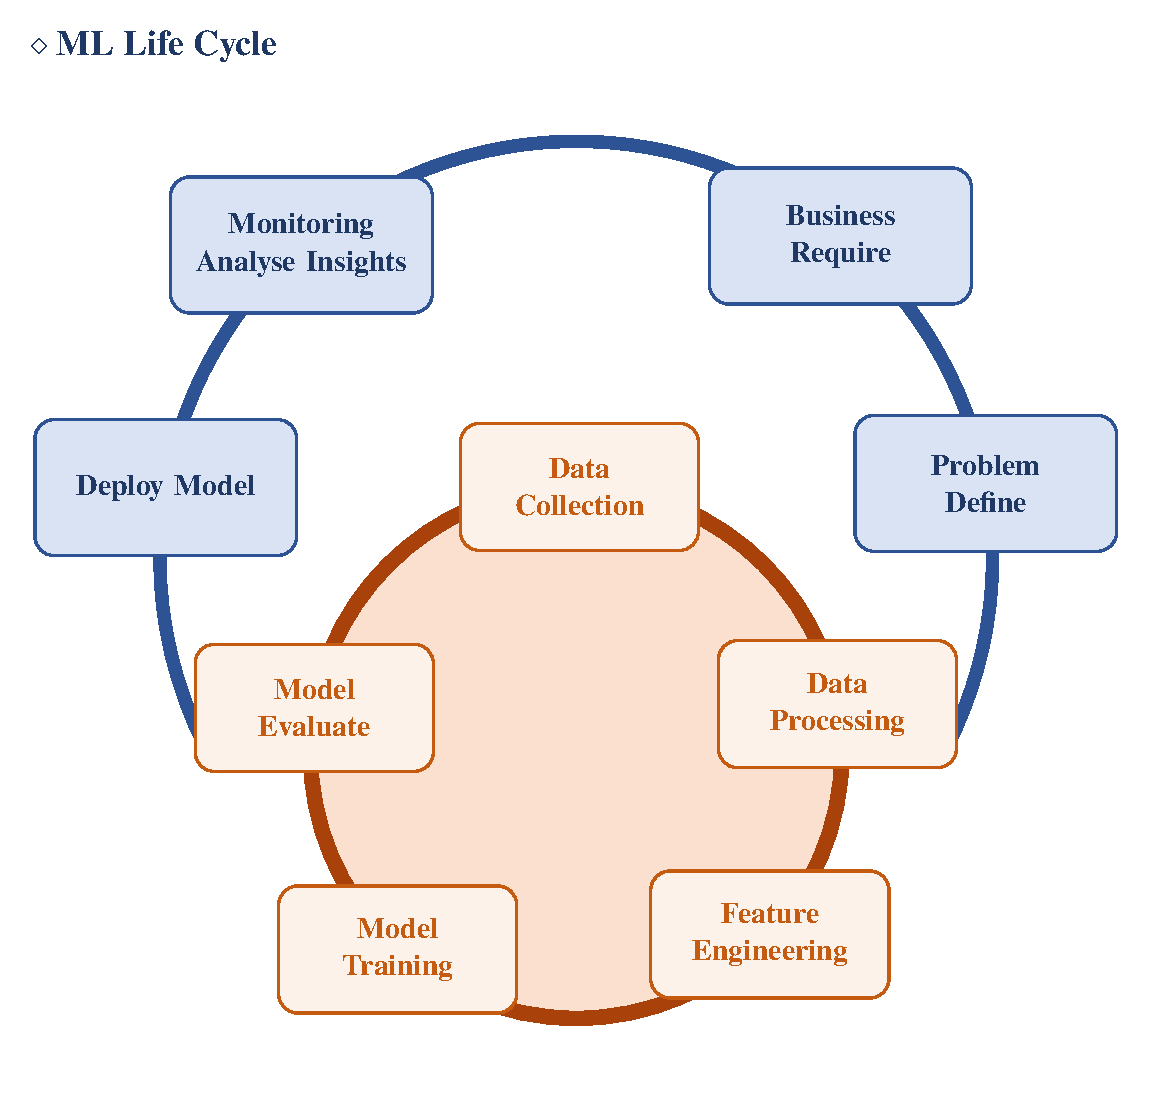
\includegraphics[width=0.78\textwidth]{sodo_ml_lifecycle_en.pdf}
    
    
    \caption[Vòng đời học máy, bản nhãn gốc tiếng Anh]{Vòng đời học máy (MLOps Lifecycle)~\cite{aivietnam2025dvc}}
    \label{fig:ml_lifecycle_en}
\end{figure}

\begin{table}[H]
\centering
\caption{Bảng đối chiếu thuật ngữ kỹ thuật MLOps Anh -- Việt}
\label{tab:mlops_terms}
\small
\renewcommand{\arraystretch}{1.2}
\begin{tabularx}{\textwidth}{@{} l l X @{}}
\toprule
\textbf{Thuật Ngữ Tiếng Anh (Gốc)} & \textbf{Thuật Ngữ Tiếng Việt} & \textbf{Ý Nghĩa Kỹ Thuật trong Dự Án} \\
\midrule
\texttt{Data Ingestion \& Versioning} & Thu nạp \& Đánh phiên bản & Lưu vết $2{,}73$ triệu dòng dữ liệu sạch bằng tệp Parquet. \\
\texttt{Causal Feature Engineering} & Kỹ nghệ đặc trưng nhân quả & Chỉ dùng dữ liệu quá khứ ($t \le T$) chống rò rỉ thông tin. \\
\texttt{Time-Series Cross Validation} & Kiểm tra chéo chuỗi thời gian & Sử dụng 3-Fold Expanding Window bảo toàn tính thứ tự thời gian. \\
\texttt{Hyperparameter Optimization} & Tối ưu hóa siêu tham số & Sử dụng thuật toán Bayesian TPE qua 20 Trials Optuna. \\
\texttt{Explainable AI (XAI)} & Trí tuệ nhân tạo giải thích được & Sử dụng SHAP TreeExplainer bóc tách mức độ đóng góp biến số. \\
\texttt{Model Serving \& Inference} & Đóng gói \& Dự báo thực thi & Module \texttt{ForecastService} phản hồi dự báo thời gian thực. \\
\bottomrule
\end{tabularx}


\end{table}


% ====================================================================
%  PHỤ LỤC D: BẢNG TRA CỨU CHI TIẾT 6 MÃ DỊ THƯỜNG KỸ THUẬT (GMM-IF)
% ====================================================================
\chapter*{Phụ lục D: Bảng Tra cứu Chi tiết 6 Mã Dị thường Kỹ thuật}
\addcontentsline{toc}{chapter}{Phụ lục D: Bảng Tra cứu Chi tiết 6 Mã Dị thường Kỹ thuật}
\label{app:outlier_matrix}
\renewcommand{\thetable}{D.\arabic{table}}
\setcounter{table}{0}
\renewcommand{\thefigure}{D.\arabic{figure}}
\setcounter{figure}{0}

Hệ thống phân lớp lai GMM--IF gán nhãn $7.431$ bản ghi dị thường ($0{,}27\%$) thành 6 mã lý do kỹ thuật phục vụ công tác O\&M hiện trường:

\begin{table}[H]
\centering
\caption{Ma trận tra cứu 6 mã dị thường kỹ thuật GMM--IF và quy trình xử lý}
\label{tab:outlier_matrix_detail}
\footnotesize
\renewcommand{\arraystretch}{1.35}
\begin{tabularx}{\textwidth}{@{} >{\raggedright\arraybackslash}p{2.9cm} >{\raggedright\arraybackslash}p{3.1cm} >{\raggedright\arraybackslash}X >{\raggedright\arraybackslash}X @{}}
\toprule
\textbf{Mã Kỹ Thuật} & \textbf{Điều Kiện Kích Hoạt} & \textbf{Bản Chất Sự Cố / Vật Lý} & \textbf{Hành Động Khuyến Nghị} \\
\midrule
\texttt{zero\_drift} & $GHI = 0\,\text{W/m}^2$, $h \le 0^\circ$,\newline $0 < E \le 0{,}025\,\text{kWh}$ & Biến dòng CT bị trôi điểm cân bằng điện áp 0V ban đêm. & Tầng ETL tự động ép về $0$; Lên lịch hiệu chuẩn biến dòng CT. \\
\midrule
\texttt{night\_leakage} & $GHI = 0\,\text{W/m}^2$, $h \le 0^\circ$,\newline $E > 0{,}025\,\text{kWh}$ & Dòng rò cảm ứng hoặc vi xử lý Inverter tiêu thụ điện tự dùng. & Kiểm tra an toàn cách điện tủ phân phối AC và chống rò. \\
\midrule
\texttt{underperformance} & $GHI \ge 500\,\text{W/m}^2$,\newline $E < 0{,}5 \times E_{\text{expected}}$ & Hỏng diode bypass, đứt cầu chì DC 1 chuỗi, hoặc cell pin bị rạn nứt. & Cử kỹ sư dùng camera nhiệt hồng ngoại quét tìm chuỗi pin lỗi. \\
\midrule
\texttt{inverter\_zero\_}\newline\texttt{output} & $GHI \ge 700\,\text{W/m}^2$,\newline $E = 0\,\text{kWh}$ & Biến tần ngắt mạch khẩn cấp do quá áp lưới ($>253\text{V}$) hoặc quá nhiệt. & Kiểm tra rơ-le bảo vệ điện áp lưới và hệ thống quạt tản nhiệt. \\
\midrule
\texttt{thermal\_}\newline\texttt{derating} & $T_{\text{amb}} \ge 40^\circ\text{C}$, $GHI \ge 800$,\newline $0{,}6 \le E/E_{\text{exp}} \le 0{,}85$ & Biến tần tự động giảm tải để bảo vệ linh kiện bán dẫn công suất IGBT. & Lắp tấm chắn nắng phản quang; vệ sinh lưới tản nhiệt biến tần. \\
\midrule
\texttt{inverter\_}\newline\texttt{clipping} & $GHI \ge 850\,\text{W/m}^2$,\newline $E \approx P_{\text{AC, max}}$ (đỉnh phẳng) & Công suất DC vượt định mức AC ($ILR = 1{,}25$). & Tối ưu kinh tế thiết kế theo chuẩn CEC; không cần can thiệp kỹ thuật. \\
\bottomrule
\end{tabularx}


\end{table}

\newpage

\begin{thebibliography}{99}
\addcontentsline{toc}{chapter}{Tài liệu Tham khảo}

% --- I. Nguồn Dữ liệu Dự án và Công trình Nghiên cứu Gốc ---
\bibitem{wimalaratne2022unisolar}
S.~Wimalaratne, D.~Haputhanthri, S.~Kahawala, G.~Gamage, D.~Alahakoon, và A.~Jennings,
\newblock ``UNISOLAR: An Open Dataset of Photovoltaic Solar Energy Generation in a Large Multi-Campus University Setting,''
\newblock \textit{15th International Conference on Human System Interaction (HSI)}, IEEE, 2022.
\newblock DOI: \href{https://doi.org/10.1109/HSI55341.2022.9869474}{10.1109/HSI55341.2022.9869474}.

\bibitem{openmeteo2023}
Open-Meteo,
\newblock ``Historical Weather API \& ERA5/ERA5-Land Reanalysis Climate Dataset,''
\newblock \textit{Open-Meteo Documentation}, 2023. [Online]. Available: \url{https://open-meteo.com/}.

\bibitem{openmeteo2025isday}
Open-Meteo,
\newblock ``Day/Night Flag (\texttt{is\_day}) Calculation Engine: Astronomical Solar Position Algorithm,''
\newblock \textit{Open-Meteo API Technical Documentation}, 2025. [Online]. Available: \url{https://open-meteo.com/en/docs}.

\bibitem{iea2023pvps}
IEA-PVPS Task 13,
\newblock ``Performance, Operation and Reliability of Photovoltaic Systems: Review of Failures and Degradation Mechanisms,''
\newblock \textit{International Energy Agency Technical Report}, IEA-PVPS T13-15:2023, 2023.

% --- II. Thuật toán Phát hiện Bất thường và Xử lý Dữ liệu ---
\bibitem{li2025gmmif}
X.~Li, G.~Du, Y.~Li, Z.~Ma, L.~Liu, M.~Jiang, F.~Liu, và T.~Mu,
\newblock ``Outlier Detection of Photovoltaic Power Generation System Data Based on GMM-IF Algorithm,''
\newblock \textit{IEEE Access}, vol.~13, pp.~108823--108837, 2025.
\newblock DOI: \href{https://doi.org/10.1109/ACCESS.2025.3581641}{10.1109/ACCESS.2025.3581641}.

\bibitem{liu2008isolation}
F.~T.~Liu, K.~M.~Ting, và Z.-H.~Zhou,
\newblock ``Isolation Forest,''
\newblock trong \textit{Proceedings of the IEEE International Conference on Data Mining (ICDM)}, 2008, pp.~413--422.

\bibitem{bishop2006pattern}
C.~M.~Bishop,
\newblock \textit{Pattern Recognition and Machine Learning},
\newblock Springer, New York, 2006.

\bibitem{tukey1977eda}
J.~W.~Tukey,
\newblock \textit{Exploratory Data Analysis},
\newblock Addison-Wesley, Reading, MA, 1977.

\bibitem{chandola2009anomaly}
V.~Chandola, A.~Banerjee, và V.~Kumar,
\newblock ``Anomaly Detection: A Survey,''
\newblock \textit{ACM Computing Surveys}, vol.~41, no.~3, pp.~1--58, 2009.

\bibitem{kim2019missing}
T.~Kim, W.~Ko, và J.~Kim,
\newblock ``Analysis and Impact Evaluation of Missing Data Imputation in Day-ahead PV Generation Forecasting,''
\newblock \textit{Applied Sciences}, vol.~9, no.~1, p.~204, 2019.
\newblock DOI: \href{https://doi.org/10.3390/app9010204}{10.3390/app9010204}.

\bibitem{fritsch1980pchip}
F.~N.~Fritsch và R.~E.~Carlson,
\newblock ``Monotone Piecewise Cubic Interpolation,''
\newblock \textit{SIAM Journal on Numerical Analysis}, vol.~17, no.~2, pp.~238--246, 1980.
\newblock DOI: \href{https://doi.org/10.1137/0717021}{10.1137/0717021}.

% --- III. Mô hình Dự báo Chuỗi Thời gian và Học máy ---
\bibitem{roy2025hourly}
M.~Roy, V.~Pyltsov, và Y.~Hu,
\newblock ``IISE PG\&E Energy Analytics Challenge 2025: Hourly-Binned Regression Models Beat Transformers in Load Forecasting,''
\newblock Columbia University, arXiv:2505.11390, 2025. [Online]. Available: \url{https://arxiv.org/abs/2505.11390}.

\bibitem{haurwitz1945}
B.~Haurwitz,
\newblock ``Insolation in Relation to Cloudiness and Cloud Density,''
\newblock \textit{Journal of Meteorology}, vol.~2, no.~3, pp.~154--166, 1945.

\bibitem{bailey2024}
M.~D.~Bailey và cộng sự,
\newblock ``Temporal and Spatial Downscaling for Solar Radiation,''
\newblock arXiv:2405.11046, 2024. [Online]. Available: \url{https://arxiv.org/abs/2405.11046}.

\bibitem{engerer2014kpv}
N.~A.~Engerer và F.~P.~Mills,
\newblock ``KPV: A clear-sky index for photovoltaics,''
\newblock \textit{Solar Energy}, vol.~105, pp.~679--693, 2014.
\newblock DOI: \href{https://doi.org/10.1016/j.solener.2014.04.019}{10.1016/j.solener.2014.04.019}.

\bibitem{dev2018tes}
S.~Dev, T.~AlSkaif, M.~Hossari, R.~Godina, A.~Louwen, và W.~van Sark,
\newblock ``Solar Irradiance Forecasting Using Triple Exponential Smoothing,''
\newblock trong \textit{IEEE International Conference on Smart Energy Systems and Technologies (SEST)}, 2018.
\newblock arXiv:1807.05872.

\bibitem{pin2025wape}
A.~Temporal-Neto và cộng sự,
\newblock ``PIN: A new metric to evaluate solar irradiance forecast models,''
\newblock \textit{Energy Reports}, vol.~13, pp.~1--12, 2025.
\newblock DOI: \href{https://doi.org/10.1016/j.egyr.2025.01.076}{10.1016/j.egyr.2025.01.076}.

\bibitem{lundberg2017shap}
S.~M.~Lundberg và S.-I.~Lee,
\newblock ``A Unified Approach to Interpreting Model Predictions,''
\newblock trong \textit{Advances in Neural Information Processing Systems (NeurIPS)}, vol.~30, 2017.
\newblock arXiv:1705.07874.

\bibitem{zhang2015metrics}
J.~Zhang, A.~Florita, B.-M.~Hodge, S.~Lu, H.~F.~Hamann, V.~Banunarayanan, và A.~M.~Brockway,
\newblock ``A suite of metrics for assessing the performance of solar power forecasting,''
\newblock \textit{Solar Energy}, vol.~111, pp.~157--175, 2015.
\newblock DOI: \href{https://doi.org/10.1016/j.solener.2014.10.016}{10.1016/j.solener.2014.10.016}.

\bibitem{zhang2013metrics}
J.~Zhang, B.-M.~Hodge, và A.~Florita,
\newblock ``Comprehensive Evaluation of Solar Irradiance and Power Forecasting Metrics,''
\newblock NREL/CP-5500-60142, \textit{3rd International Workshop on Integration of Solar Power into Power Systems}, 2013.

\bibitem{lonij2012tucson}
V.~P.~Lonij, A.~E.~Brooks, K.~Koch, và A.~D.~Cronin,
\newblock ``Analysis of 80 Rooftop PV Systems in the Tucson, AZ Area,''
\newblock trong \textit{38th IEEE Photovoltaic Specialists Conference (PVSC)}, 2012, pp.~549--553.
\newblock DOI: \href{https://doi.org/10.1109/PVSC.2012.6317674}{10.1109/PVSC.2012.6317674}.

\bibitem{taylor2018prophet}
S.~J.~Taylor và B.~Letham,
\newblock ``Forecasting at Scale,''
\newblock \textit{The American Statistician}, vol.~72, no.~1, pp.~37--45, 2018.

\bibitem{box2015time}
G.~E.~P.~Box, G.~M.~Jenkins, G.~C.~Reinsel, và G.~M.~Ljung,
\newblock \textit{Time Series Analysis: Forecasting and Control}, 5th ed.,
\newblock John Wiley \& Sons, Hoboken, NJ, 2015.

\bibitem{ke2017lightgbm}
G.~Ke, Q.~Meng, T.~Finley, T.~Wang, W.~Chen, W.~Ma, Q.~Ye, và T.-Y.~Liu,
\newblock ``LightGBM: A Highly Efficient Gradient Boosting Decision Tree,''
\newblock trong \textit{Advances in Neural Information Processing Systems (NeurIPS)}, vol.~30, 2017, pp.~3146--3154.

\bibitem{chen2016xgboost}
T.~Chen và C.~Guestrin,
\newblock ``XGBoost: A Scalable Tree Boosting System,''
\newblock trong \textit{Proceedings of the ACM SIGKDD International Conference on Knowledge Discovery and Data Mining}, 2016, pp.~785--794.

\bibitem{aivietnam2025dvc}
Đặng Nhã và Anh Dương,
\newblock ``Data Version Control,''
\newblock tài liệu bài giảng \textit{AI VIET NAM --- All-in-One 2025}, slide~9 (\textit{Theory Perspective --- ML Life Cycle}), 2025.

\bibitem{kolassa2007mad}
S.~Kolassa và W.~Schütz,
\newblock ``Advantages of the MAD/Mean ratio over the MAPE,''
\newblock \textit{Foresight: The International Journal of Applied Forecasting}, no.~6, pp.~40--43, 2007.

\bibitem{nguyen2026meta}
T.~N.~Nguyen và F.~Müsgens,
\newblock ``A meta-analysis of solar forecasting based on skill score,''
\newblock \textit{Journal of Renewable and Sustainable Energy}, vol.~18, no.~2, p.~026102, 2026.
\newblock DOI: \href{https://doi.org/10.1063/5.0300682}{10.1063/5.0300682}.

\bibitem{marquez2013skill}
R.~Marquez và C.~F.~M.~Coimbra,
\newblock ``Proposed Metric for Evaluation of Solar Forecasting Models,''
\newblock \textit{Journal of Solar Energy Engineering} (ASME), vol.~135, no.~1, p.~011016, 2013.
\newblock DOI: \href{https://doi.org/10.1115/1.4007496}{10.1115/1.4007496}.

\bibitem{wwrp2009verif}
WWRP/WGNE Joint Working Group on Forecast Verification Research,
\newblock ``Forecast Verification: Issues, Methods and FAQ,''
\newblock Bureau of Meteorology, Australia, 2009. [Online]. Available: \url{https://www.cawcr.gov.au/projects/verification/verif_web_page.html}.

% --- IV. Kiến trúc Kho Dữ liệu, API và Công cụ Trực quan hóa ---
\bibitem{kimball2013dwh}
R.~Kimball và M.~Ross,
\newblock \textit{The Data Warehouse Toolkit: The Definitive Guide to Dimensional Modeling}, 3rd ed.,
\newblock John Wiley \& Sons, Indianapolis, IN, 2013.

\bibitem{wmo2021guide}
World Meteorological Organization (WMO),
\newblock \textit{Guide to Instruments and Methods of Observation: Volume I -- Measurement of Meteorological Variables},
\newblock WMO-No. 8, Geneva, Switzerland, 2021.

\bibitem{supabase2024}
Supabase Inc.,
\newblock ``PostgreSQL Database \& Row-Level Security for Modern Analytics Architecture,''
\newblock \textit{Supabase Technical Architecture Documentation}, 2024. [Online]. Available: \url{https://supabase.com/docs}.

\bibitem{pedregosa2011sklearn}
F.~Pedregosa et~al.,
\newblock ``Scikit-learn: Machine Learning in Python,''
\newblock \textit{Journal of Machine Learning Research}, vol.~12, pp.~2825--2830, 2011.

\bibitem{tableau2023guidelines}
Tableau Software (Salesforce),
\newblock \textit{Visual Analysis Best Practices: A Guide to Creating Meaningful Dashboards},
\newblock Seattle, WA, 2023.

\bibitem{holmgren2018pvlib}
W.~F. Holmgren, C.~W. Hansen, and M.~A. Mikofski,
\newblock ``pvlib python: a python package for modeling solar energy systems,''
\newblock \textit{Journal of Open Source Software}, vol.~3, no.~29, p.~884, 2018.

\bibitem{noaa_solar}
NOAA Global Monitoring Laboratory,
\newblock ``Solar Calculation Details and Solar Position Algorithm,''
\newblock \textit{National Oceanic and Atmospheric Administration (NOAA) Earth System Research Laboratories}, 2024. [Online]. Available: \url{https://gml.noaa.gov/grad/solcalc/calcdetails.html}.

\end{thebibliography}


\end{document}
